
\chapter{Measurement of the \tty cross-sections} % Main chapter title
\label{Chapter3} % Change X to a consecutive number; for referencing this chapter elsewhere, use \ref{ChapterX}

\section{Fiducial phase space}
\label{sec:fiducial-phase-space}
The measurements are performed at particle level in a fiducial phase space volume. Particle level refers to final state particles after the parton showering and hadronization but prior to any interaction with the detector apparatus. The fiducial regions in the single lepton and dilepton final states are defined to closely follow the kinematic requirements at reconstruction level. The objects are defined as follows:
\begin{itemize}
\item Photons: Photons are required to not originate from a hadron decay, to have $p_T > \SI{20}{\GeV}$ and $|\eta| < \SI{2.37}{}$ and to be isolated such that the sum of transverse momenta of all charged particles surrounding the photon within $\Delta R \leq$ 0.2 must be smaller than 5\% of its own \pt.
\item Leptons: Electrons and muons are dressed with close by photons (photons which are not originating
from hadrons, in a $\Delta R <0.1$ cone around the lepton). Leptons are required to have \pt $>$ 25 GeV
and $|\eta|<$ 2.5, and not being originated from hadron decays.
\item Jets: Jets are clustered with the anti-kt algorithm with a radius of R = 0.4. Non-interacting particles and
muons are not considered in the clustering. Jets are required to have \pt $>$ 25 GeV
and $|\eta|<$ 2.5
\item b-jets: A particle-level jet is identified as a $b$-jet if a hadron with $\pT > \SI{5}{\GeV}$ containing a $b$-quark is matched to the jet through a ghost-matching method~\cite{Cacciari:2008gn}.
\item The overlap removal among the different objects is performed in the following order:
\begin{itemize}
\item Muon-jet: Jets with $\Delta R(\mu, j)\leq 0.4$ are removed.
\item Electron-jet: Jets with $\Delta R(e, j)\leq 0.4$ are removed.
\item Photon-jet: Jets within $\Delta R( j, \gamma) \leq 0.4$ of an isolated photon are removed.
\end{itemize}
\end{itemize}

The fiducial phase space in the single-lepton channel is defined by requiring exactly one photon, exactly one electron or muon, at least four jets among which at least one is a $b$-jet. In the case of the dilepton channels, it is defined by requiring exactly one photon, exactly two leptons (electron or muon), at least two jets among which at least one is a $b$-jet.



\section{Differential cross-section measurement}
\label{sec:diff-xsec-measurement}
The cross-section is measured within a defined fiducial phase space volume (\cref{sec:fiducial-phase-space}) at particle level as a function of different observables listed in \cref{tab:listvariables}. The cross-section at the particle level is derived using an unfolding technique. Unfolding is used to extract the truth spectrum from the reconstruction level spectrum correcting the detector effects such as limited resolutions, efficiency and acceptance effects, making the results easier to compare with the theoretical predictions. We implement the profile likelihood unfolding method for this purpose, detailed in \cref{sec:profile-likelihodd-unfolding}. 

Ideally, a continuous functional dependence of the measurement would be preferable. However, the finite detector resolution prevents this. Consequently, we measure the cross-section in discrete bins. For more information on how the bins are chosen detailed in \cref{sec:choice-of-binning}.

\begin{table}[ht]
\caption{The differential cross sections are measured in single-lepton channel and dilepton channel as a function of the following variables: }
\label{tab:listvariables}
\begin{footnotesize}
\begin{tabular} {r l }
  Symbol & Defintion \\
  \hline
  Both dilepton and single lepton channels: & \\
  \hline 
  \pt($\gamma$) & Transverse momentum of photon \\ 
  $|\eta|$($\gamma$) & Absolute value of the pseudorapidity of the photon \\
  \DRlph & Angular separation between the photon and the closest lepton \\
  $\Delta R_{min}(\gamma, b)$ &  Angular separation between the photon and the closest $b$ jet \\
  $\Delta R_{min}(l, j)$ & Smallest angular separation between any of the selected leptons and jets \\
  $p_T(j_1)$ & Transverse momentum of the leading jet\\

  \hline
  Additional variables for dilepton channel: & \\
  \hline
  $\Delta R(\gamma, l_1)$ & Angular separation between the photon and the leading lepton\\
  $\Delta R(\gamma, l_2)$ & Angular separation between the photon and the subleading lepton\\
  \Detall & Pseudorapidity difference between the two leptons\\
  \Dphill & Azimuthal angle difference between the two leptons\\
  $p_T(l,l)$ & Transverse momentum of the dilepton system\\
  $p_T(j_1)$ & Transverse momentum of the leading jet\\
    
\end{tabular}

\end{footnotesize}
\end{table}
\FloatBarrier

As detailed in profile-likelihood unfolding section[\ref{sec:profile-likelihodd-unfolding}], the histogram templates at the reconstruction level are used as the inputs for the unfolding, where the signal histograms are obtained by folding the truth distributions with the response matrix. To take into account the uncertainties response matrices are constructed for every source of systematic uncertainties for signal and varied histogram templates (at the reconstruction level) are produced for background templates. More details on how the truth distributions and response matrices are constructed are detailed in \cref{sec:inputs-for-unfolding}.

Before the unfolding procedure is applied to the real data various tests are performed beforehand using the pseudo-data. This approach validates the unfolding procedure and avoids any post-unfolding modifications to the model, which could introduce bias. Here pseudo-data refers to the sum of all MC templates including signal and backgrounds. Two tests are performed, closure test and stress test. In the closure test, the pseudo-data is unfolded and compared with the truth distribution of the signal, and a good closure is observed (more on closure test in \cref{sec:closure_test}). This validates that the unfolding procedure using response matrix and truth distribution can correctly measure the signal from the dataset (in this case pseudo-dataset). The signal normalization and shape shape in real data can be different than in MC simulation. Unfolding using MC truth distribution and response matrix (which is derived from MC simulation) can introduce bias while measuring the signal from the real data. The stress test mentioned in \cref{sec:stress_test} validates that the unfolding procedure is very robust and can measure the signal correctly from the data even if the shape of the signal present in the data is different than in MC simulation. 

After validating the unfolding procedure, fit and unfolding is performed on the real data to measure the cross-section. The results are detailed in \cref{sec:tty_prod_measurement}, \cref{sec:tty_total_measurement} and \cref{sec:tty_prod_sldl_measurement} for \tty production measurement, inclusive \tty measurement and \tty production measurement in a combined single lepton and dilepton channel respectively.

\subsection{Profile likelihood unfolding}
\label{sec:profile-likelihodd-unfolding}
The reconstruction level spectrum $y$ can be written in terms of the truth spectrum $x$ as $$ y = R x$$, where $R$ is the response matrix. The standard unfolding procedure involves the inversion of the response matrix to obtain the truth spectrum. It becomes difficult when the matrix is not easily invertible. Instead, we follow a different approach in which standard profile likelihood fitting is used for unfolding ~\cite{cls_3}. 
The TRExFitter framework \emph{TRexFitter}\footnote{\url{https://trexfitter-docs.web.cern.ch/trexfitter-docs/}} is used for the fitting and unfolding process. In this approach, the truth distribution comprising N bins is multiplied by the corresponding response matrix (\cref{sec:inputs-for-unfolding}) of size N x M, thereby transforming the truth distribution into a reconstruction level distribution with M bins. A normalization factor is assigned for each bin of the truth distribution, these factors are parameters of interest (POI). It is important to note that the normalization of these folded distributions on the reconstruction level is identical to the normalization of the truth distribution. Therefore, by measuring the normalization factors for each bin of each folded distribution on the reconstruction level, the normalization of the truth level is directly obtained, thus we obtain the cross-section at the truth level. Standard profile likelihood fit is performed on reconstruction level distribution to obtain the POIs. A toy example to illustrate the unfolding procedure is shown in Figure~\ref{fig:unfolding_toy_example}.

%generate code to add a figure
\begin{figure}[ht]
    \centering
    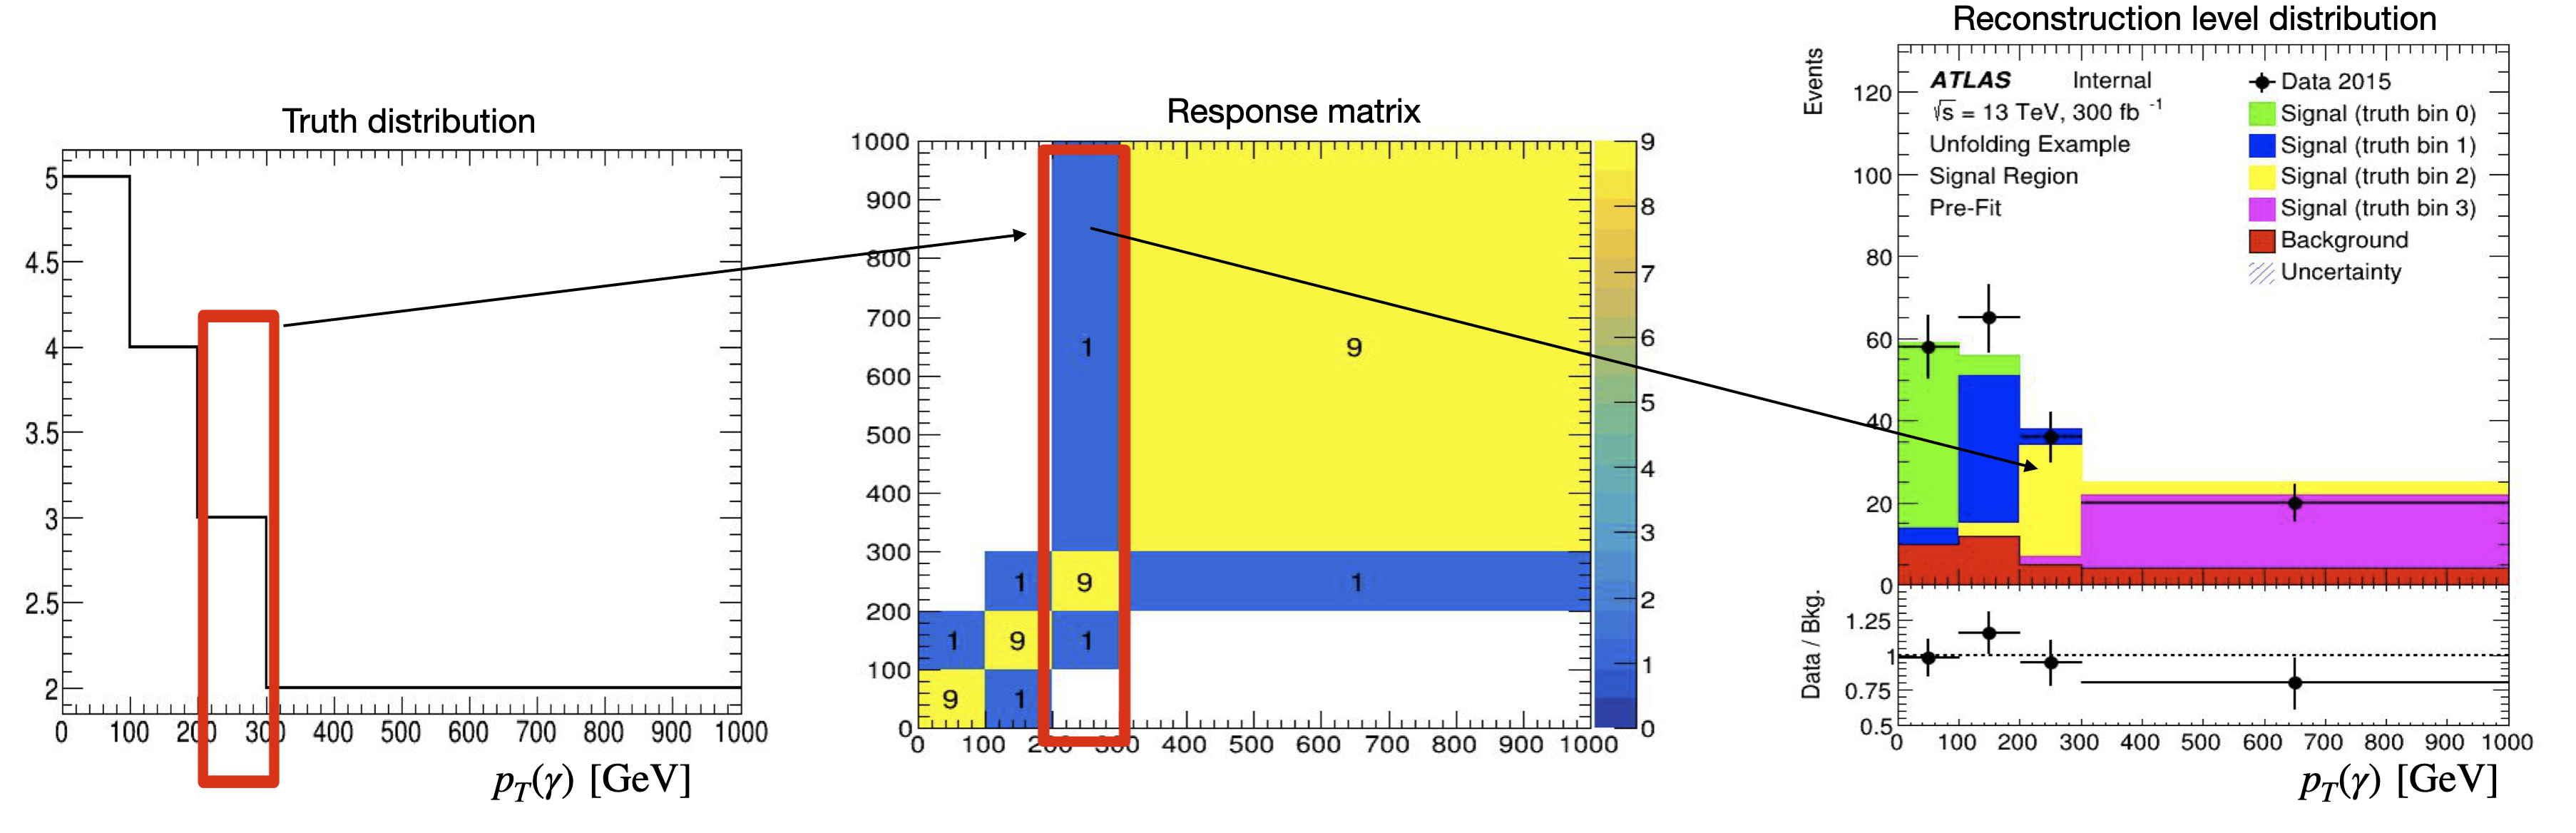
\includegraphics[width=0.9\textwidth]{figures/toy_profile_likelihood_fit.png}
    \caption{Toy example to illustrate the unfolding procedure. The truth distribution is multiplied by the response matrix to obtain the distribution at the reconstruction level. A normalization factor is assigned for each bin of the truth distribution. Profile likelihood fit is performed to the reconstruction level distribution to obtain the normalization factors. The truth distribution is directly obtained from the normalization factors.}

    \label{fig:unfolding_toy_example}
\end{figure}
\FloatBarrier

The likelihood is constructed using the signal and background templates in the following way:
\begin{equation}\label{eq:likelihodd-defn}
	L(\vec{n}^{data} | \vec{k}, \vec{\theta}) = \prod_{\mathrm{c} \epsilon \mathrm{Region}} \quad \prod_{\mathrm{b} \epsilon \mathrm{Bins}} \mathrm{Pois} (n^{\mathrm{data}}_{b,c}|\nu_{b,c}(\vec{k}, \Vec{\theta})) \cdot \prod_{p} \mathrm{Gauss}(0|\theta_{p},1)
\end{equation}

where, \textit{Region} refers to the different signal and control regions, \textit{Bins} refers to the bin of the reconstruction level histogram, $n^{\mathrm{data}}_{b,c}$ is the data in bin \textit{b} and region \textit{c}, $\nu_{b,c}$ is the expected total events in bin \textit{b} and channel \textit{c}. $\Vec{\theta}$ are the constrained nuisance parameter describing systematic uncertainties \cref{sec:sources-of-uncertainties} and $\mathrm{Gauss}(0|\theta_p,1)$ is a Gaussian constraint of the NP $\theta_p \in \vec{\theta}$ with mean of 0 and standard deviation of 1, $\vec{k}$ are the unconstrained parameters (e.g. POIs).

$\nu_{b,c}$ can be expressed as follows:

\begin{align}\label{eq:likelihodd-defn-1}
    \nu_{b,c} = \left[\sum_i \gamma_{b,c,i} \cdot \mu_{i} \cdot R_{b,c,i} \cdot T_{i}\right] + \sum_{B} \gamma_{b,c}^{B} \times N_{b,c}^{B} 
\end{align}

where, $\gamma$ factors are the bin-by-bin scale factors for MC statistical uncertainties. The background samples each have the factors $\gamma_{b,c}^{B}$ and for the signal, each truth bin has a unique $\gamma_{b,c,t}$. $R_{b,c,t}$ are the response matrices of the signal, calculated from the particle level and reconstruction level events. $\mu_{i}$ corresponds to the signal strength of the bin $T_{i}$ at particle level.

Subsequently, a Profile Likelihood fit is performed with this Likelihood in \emph{TRexFitter}\footnote{\url{https://trexfitter-docs.web.cern.ch/trexfitter-docs/}}.

% mention the later story, the minimization and so on.
% put more details on the fit and unfolding?
% Also how the uncertainties are taken into account in the likelihood function
% with which errors are calculated also



\subsection{Choice of binning}
\label{sec:choice-of-binning}
The choice of the binning depends on several factors, the bin width of each bin must be greater than the resolution of the observable in that range and the statistical uncertainties in every bin of the measured distribution are small enough to avoid large fluctuations. To achieve this, two criteria were chosen to determine the bin widths. The bin width is chosen such that it is larger than twice the resolution of the observable and that the expected statistical uncertainty in the measured distribution is below 10\%. The algorithm starts with a finer binned histogram at the reconstruction level and starts to merge the bin from left to right till the statistical uncertainty reaches below 5-7\% (depending on the observable). This process is performed only considering the signal region (at the reconstruction level) due to the complexity of the profile likelihood unfolding across multiple reconstruction regions. After determining the binning edges through the algorithm, the fit and unfolding are performed and finally the statistical uncertainty is verified at the unfolded distribution. A crucial consideration is that the binning choice should exceed twice the resolution of the variable, as stated above. The resolution for the variable $\pt(\gamma)$, $|\eta(\gamma)|$, $\Delta R(\gamma,l)$, $\Delta R(\gamma,b)$, $\Delta R_{min}(l,j)$, $\Delta \eta(l,l)$, $\Delta \phi(l,l)$, $\pt(j_1)$, $\pt(l,l)$ are found to be around 1-2 GeV, 0.1-0.15, 0.005-0.008, 0.014-0.020, 0.01, 0.0006, 0.0003, 10 GeV, 2-3 GeV, respectively. The optimized bin widths based on the statistical uncertainty fullfilled in all cases the resolution criterion. During binning optimization, we observed slight statistical fluctuations in some bins, which can be attributed to the complexities of fit and unfolding across regions. For those cases the bin boundaries were slightly adjusted as well as to have simpler bin edges (e.g. multiples of 0.1, 5, 10 depending on the distribution). 

This study is performed for \tty(prod) and \tty(total) measurements in dilepton channel. The results are compared among the two sets and with the binning used by CMS measurement ~\cite{CMS2022}. The bin boundaries showed significant similarities. Testing our unfolding setup against CMS binning revealed that the unfolded distributions met the set criteria, yielding in general similar uncertainties and migrations. Consequently, we adopted the CMS binning, allowing a more conducive comparison in the future. For illustration, the resolution and comparison of two setups for some example variables can be found in appendix~\ref{sec:binning_optimization_study}. The same binning was applied to the l+jets channel. 

The unfolded $\pt(\gamma)$ distribution is used as input for the EFT measurement combining the single lepton and dilepton fiducial phase spaces as mentioned in section {ToDo: add ref}. The binning for this variable was revised to improve the sensitivity in the EFT measurement, increasing the number of bins while keeping the total expected uncertainty in the tail of the distribution around 10\%, which is most sensitive to the EFT parameters.  



\subsection{Inputs for unfolding}
\label{sec:inputs-for-unfolding}
As inputs to the unfolding, binned distribution of the observable at particle level as well as the response matrix are needed. Binned distributions at the particle level are obtained after applying the particle level event selection outlined in \cref{sec:event-selection}. These distributions are depicted in \cref{fig:folding_input_ljet} for the single lepton channel and in \cref{fig:folding_input_dilep1} for the dilepton channel. The bin content, represented by $T_{i}$, serves as input for the Likelihood function described in \cref{eq:likelihodd-defn-1}.

\paragraph{Response matrix} The response matrix effectively translates particle level distribution to the reconstruction level distribution taking into account factors like selection efficiency, detector acceptance and migration of events to neighboring bins. Essentially, when the response matrix is applied to the truth distribution it yields distribution at the reconstruction level. Response matrix is constructed from particle level to each region in reconstruction level, resulting in 4 response matrices for single lepton channel and 2 for dilepton channel. Furthermore, response matrices are obtained for each source of uncertainty. These matrices are formulated using the migration matrix ($N_{r \cap t}$), which relates the reconstructed and truth level distributions for the respective variable, along with the corresponding truth ($N_{t}$) and reconstructed ($N_{r}$) distributions in the following way:
\begin{align}
    \text{Response, } P_{r,t} = \frac{M_{\mathrm{r,t}} \times \epsilon_{t}}{f_{r}}\\
    = \frac{\frac{N_{r \cap t}}{\sum_{r} N_{r \cap t}} \times \frac{\sum_{r} N_{r \cap t}}{N_{t}}}{\frac{\sum_{t} N_{r \cap t}}{N_{r}}}\\
    = N_{r \cap t} \times \frac{N_{r}}{N_{t}\times \sum_{t} N_{r \cap t}}
\end{align}

where, \\
$M_{\mathrm{r,t}}$ is the normalised Migration matrix (as shown in \cref{fig:folding_input_migration_dilep}, \cref{fig:folding_input_migration_ljet}),\\
$\epsilon_{t}$ is the efficiency of the truth events and \\
$f_{r}$ is the acceptance of the reconstructed events

\vspace*{20pt}

For illustration, the normalized migration matrices for $p_T(\gamma)$ in the different signal and control regions are shown in \cref{fig:folding_input_migration_ljet} and \cref{fig:folding_input_migration_dilep} for the single lepton and dilepton channels, respectively. The response matrices for $p_T(\gamma)$  are shown in \cref{fig:folding_input_response_ljet_pt1} and \cref{fig:folding_input_response_dilep} for single channel and dilepton channel respectively. Additionally in \cref{fig:folding_input_response_ljet_pt1} and \cref{fig:folding_input_response_dilep} data-MC Comparison plots are shown where the signal is reconstructed by folding the truth distribution with the response matrix. 

The signal histogram is obtained at the reconstruction level using truth distribution and response matrix. The histogram templates for backgrounds are also used as inputs for the fit and unfolding. The background templates are constructed using the MC samples described in [todo ref] and applying the signal and control region selection criteria and merged into categories as described in the \cref{sec:photon-categorisation}. The background templates enter in the likelihood function following the equation \cref{eq:likelihodd-defn-1}.
%The migration matrices, response matrices and data-MC comparison plots for other observables are shown in Section ~\ref{sec:results_others_ljet} for the single lepton channel and in Section ~\ref{sec:results_others_dilep} for the dilepton channel.




\begin{figure}[ht]
    \centering
    % ph pt
    \subfloat[]{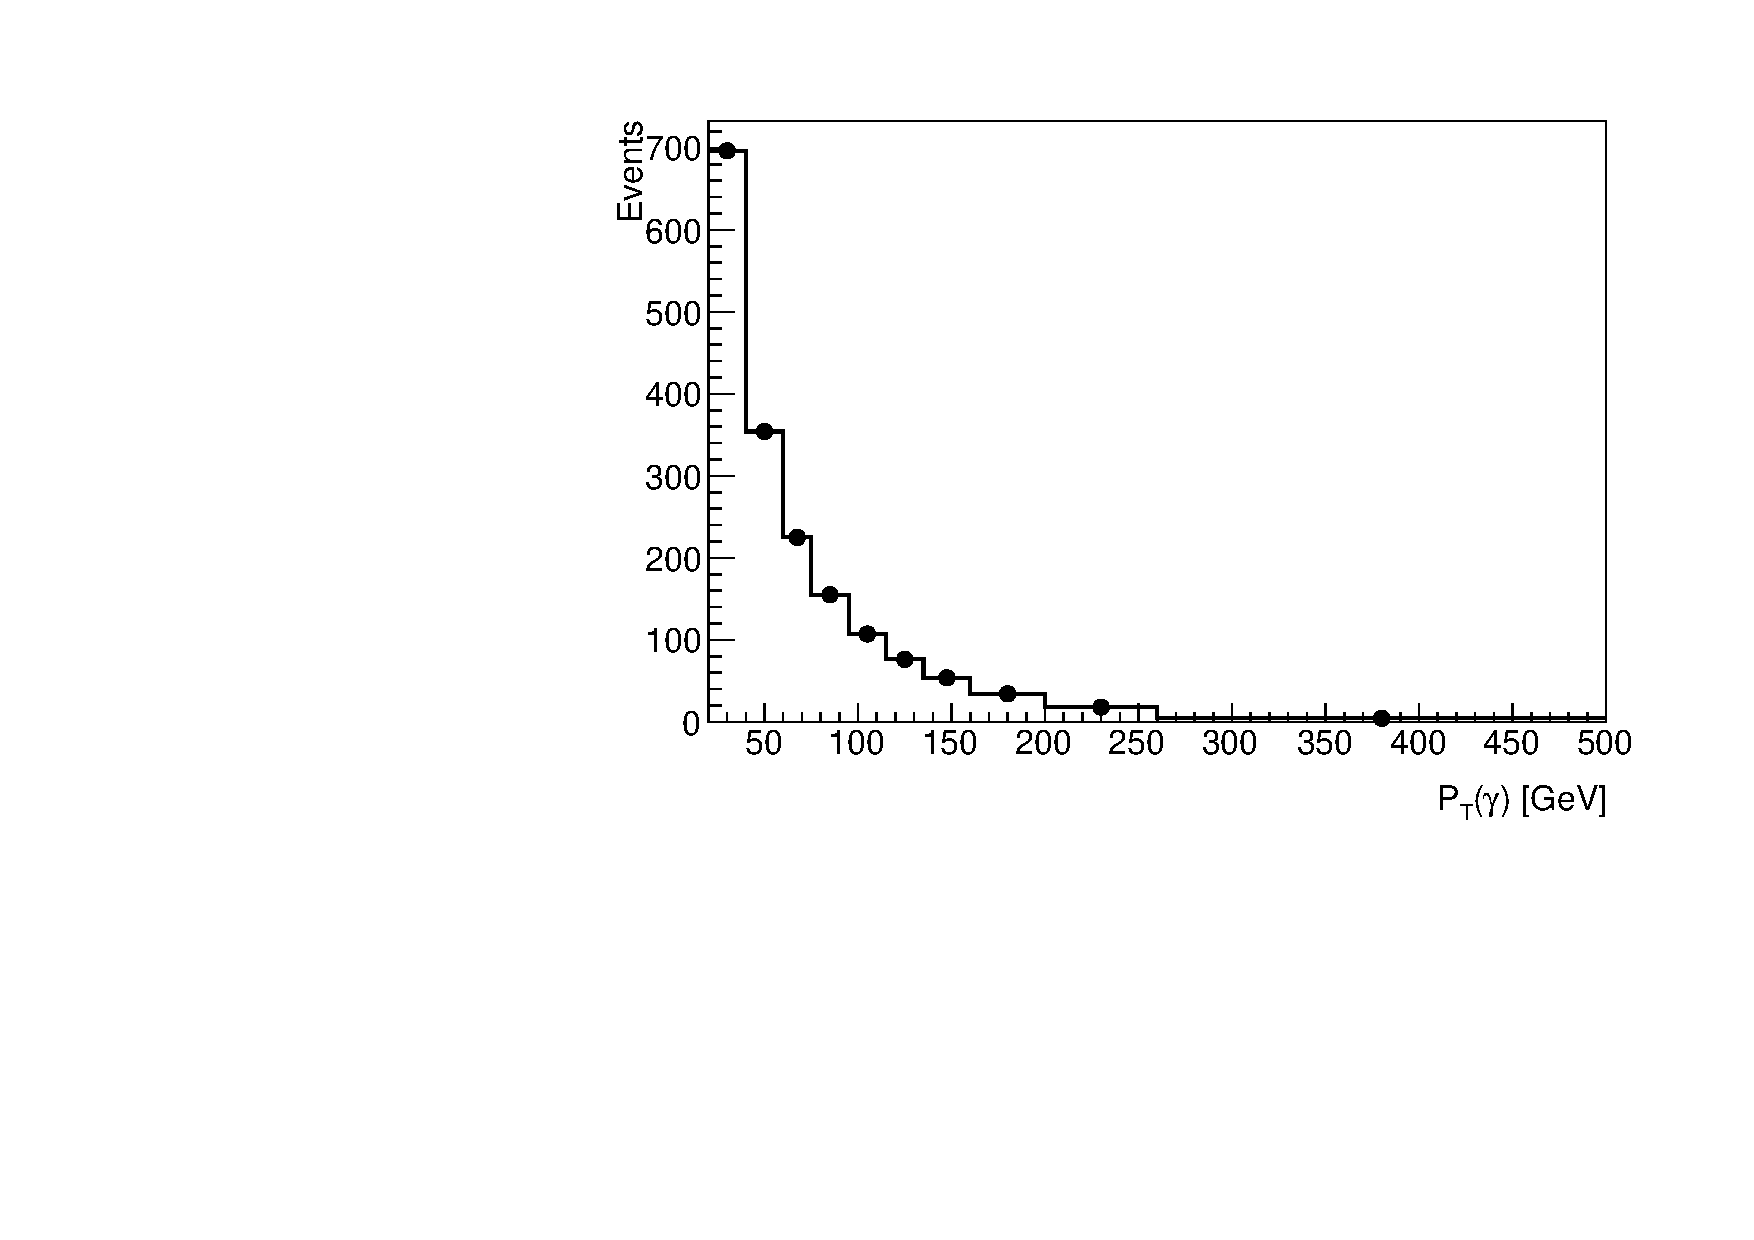
\includegraphics[width=0.3\textwidth]{figures/diff_xsec/ljet/Truth_dist/tty1l_pt_all_syst_Unfolding_truth_distribution.pdf}}
    \quad
    % ph eta
    \subfloat[]{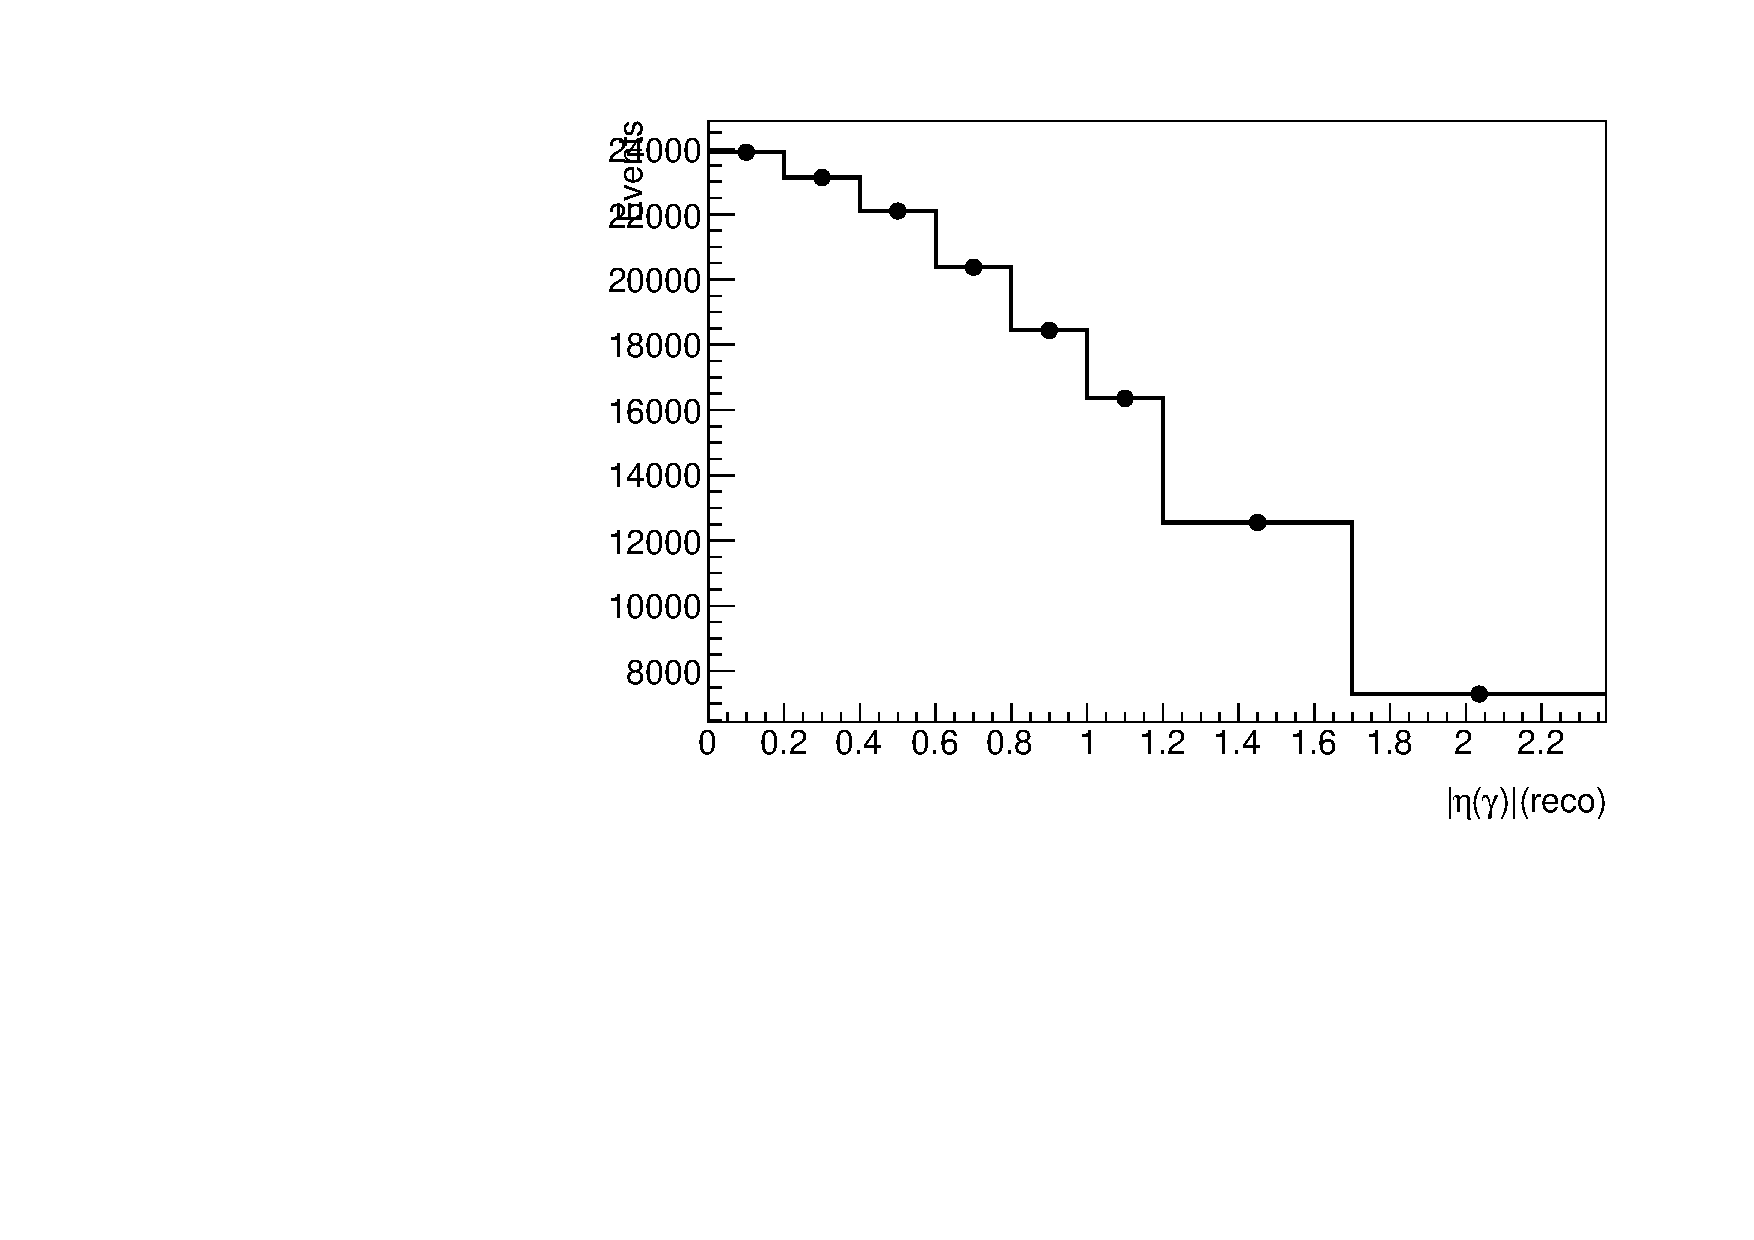
\includegraphics[width=0.3\textwidth]{figures/diff_xsec/ljet/Truth_dist/tty1l_eta_all_syst_Unfolding_truth_distribution.pdf}}
    \quad
    % delta R (ph, l)
    \subfloat[]{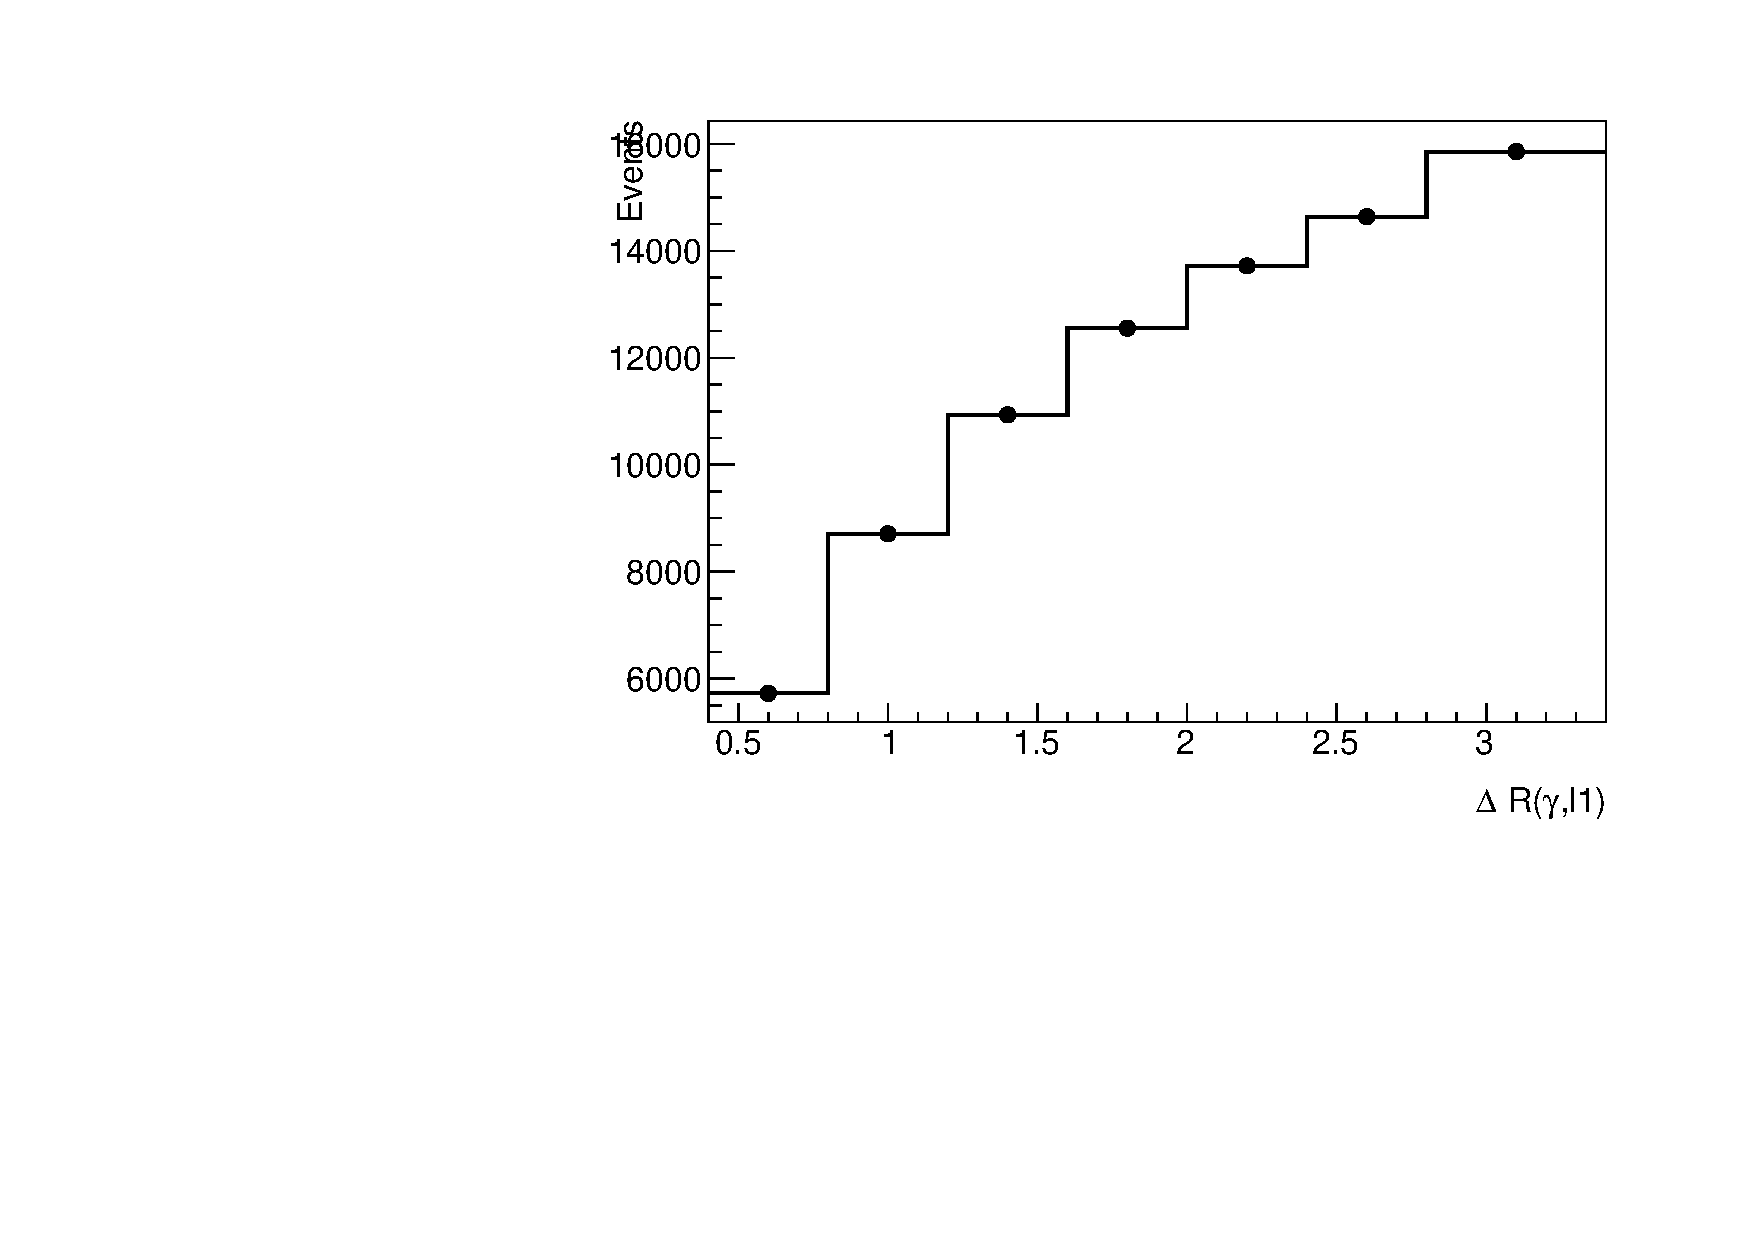
\includegraphics[width=0.3\textwidth]{figures/diff_xsec/ljet/Truth_dist/tty1l_dr_all_syst_Unfolding_truth_distribution.pdf}}
    \quad
    % delta R (ph, b)
    \subfloat[]{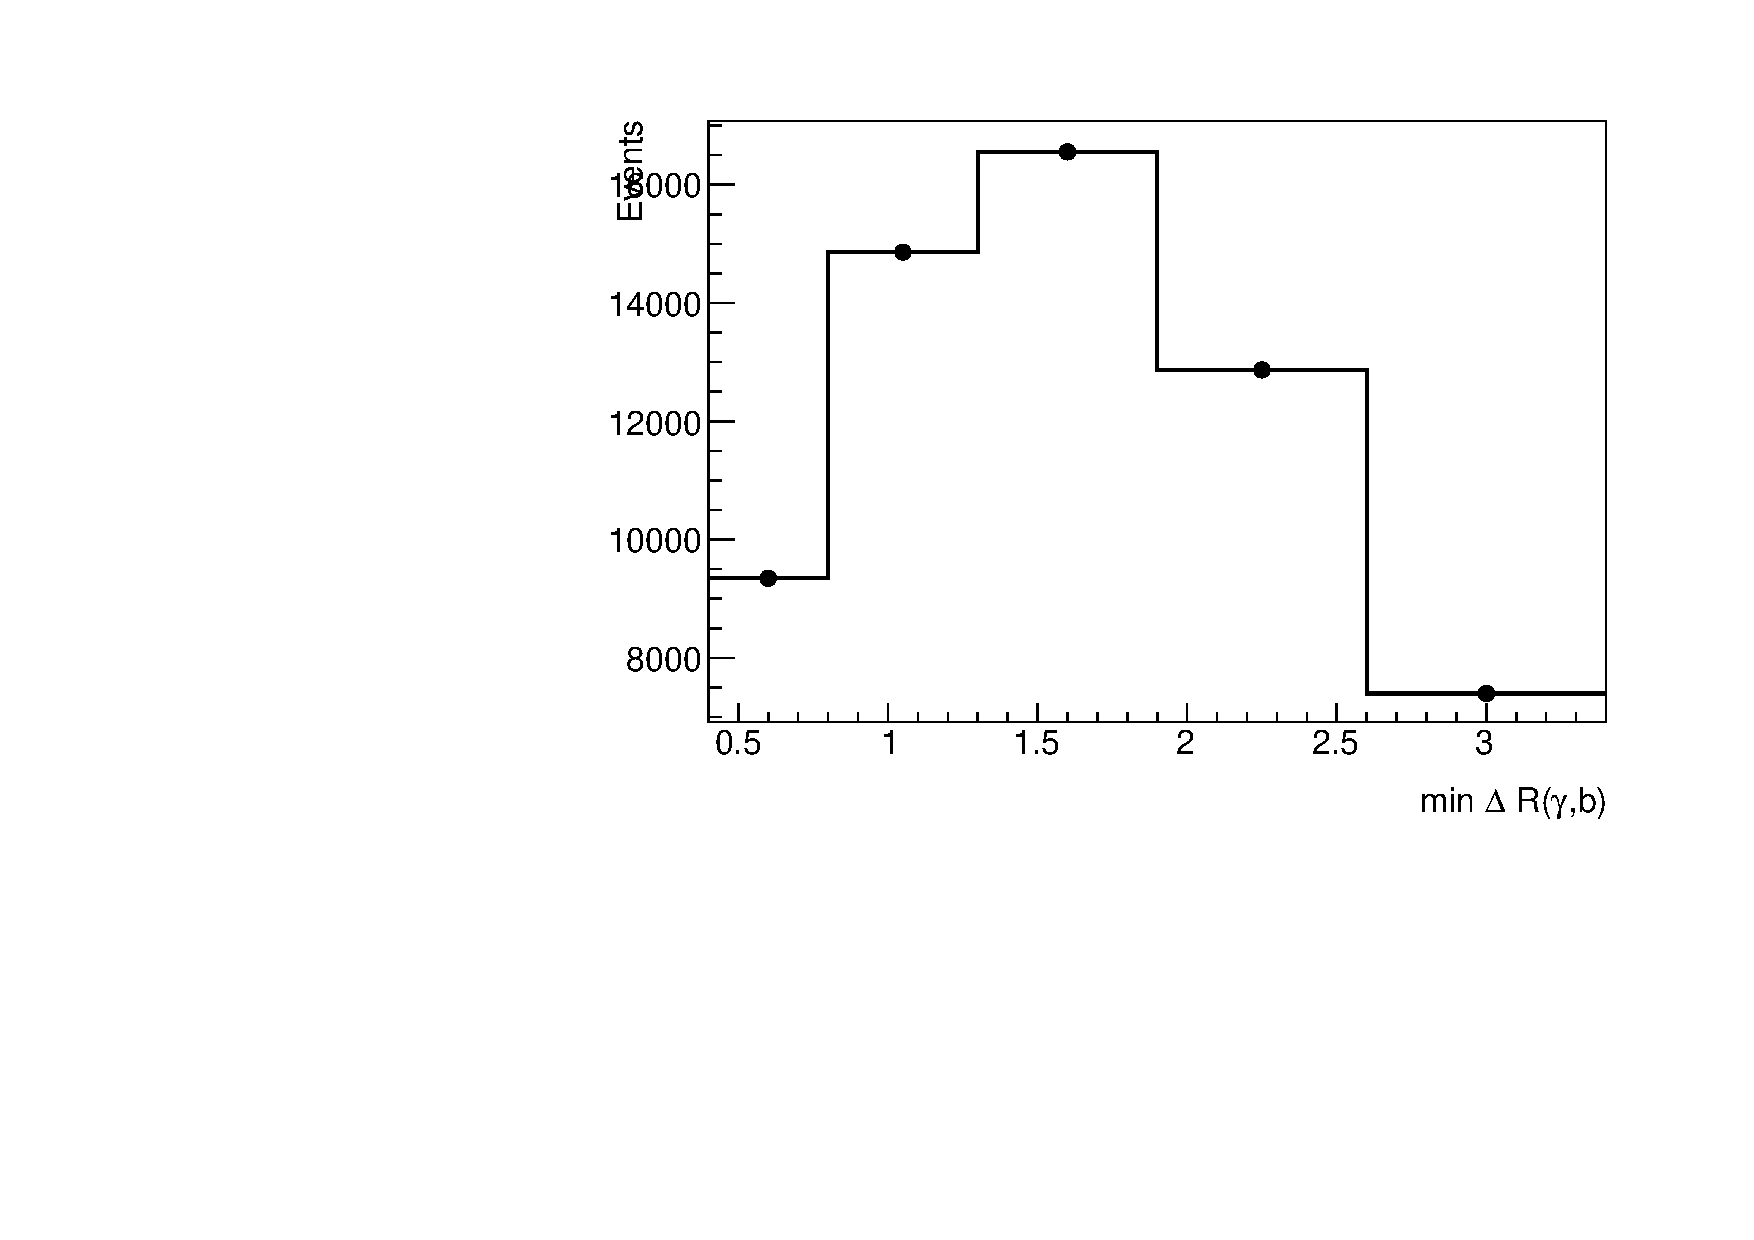
\includegraphics[width=0.3\textwidth]{figures/diff_xsec/ljet/Truth_dist/tty1l_drphb_all_syst_Unfolding_truth_distribution.pdf}}
    \quad
    % delta R(lj)
    \subfloat[]{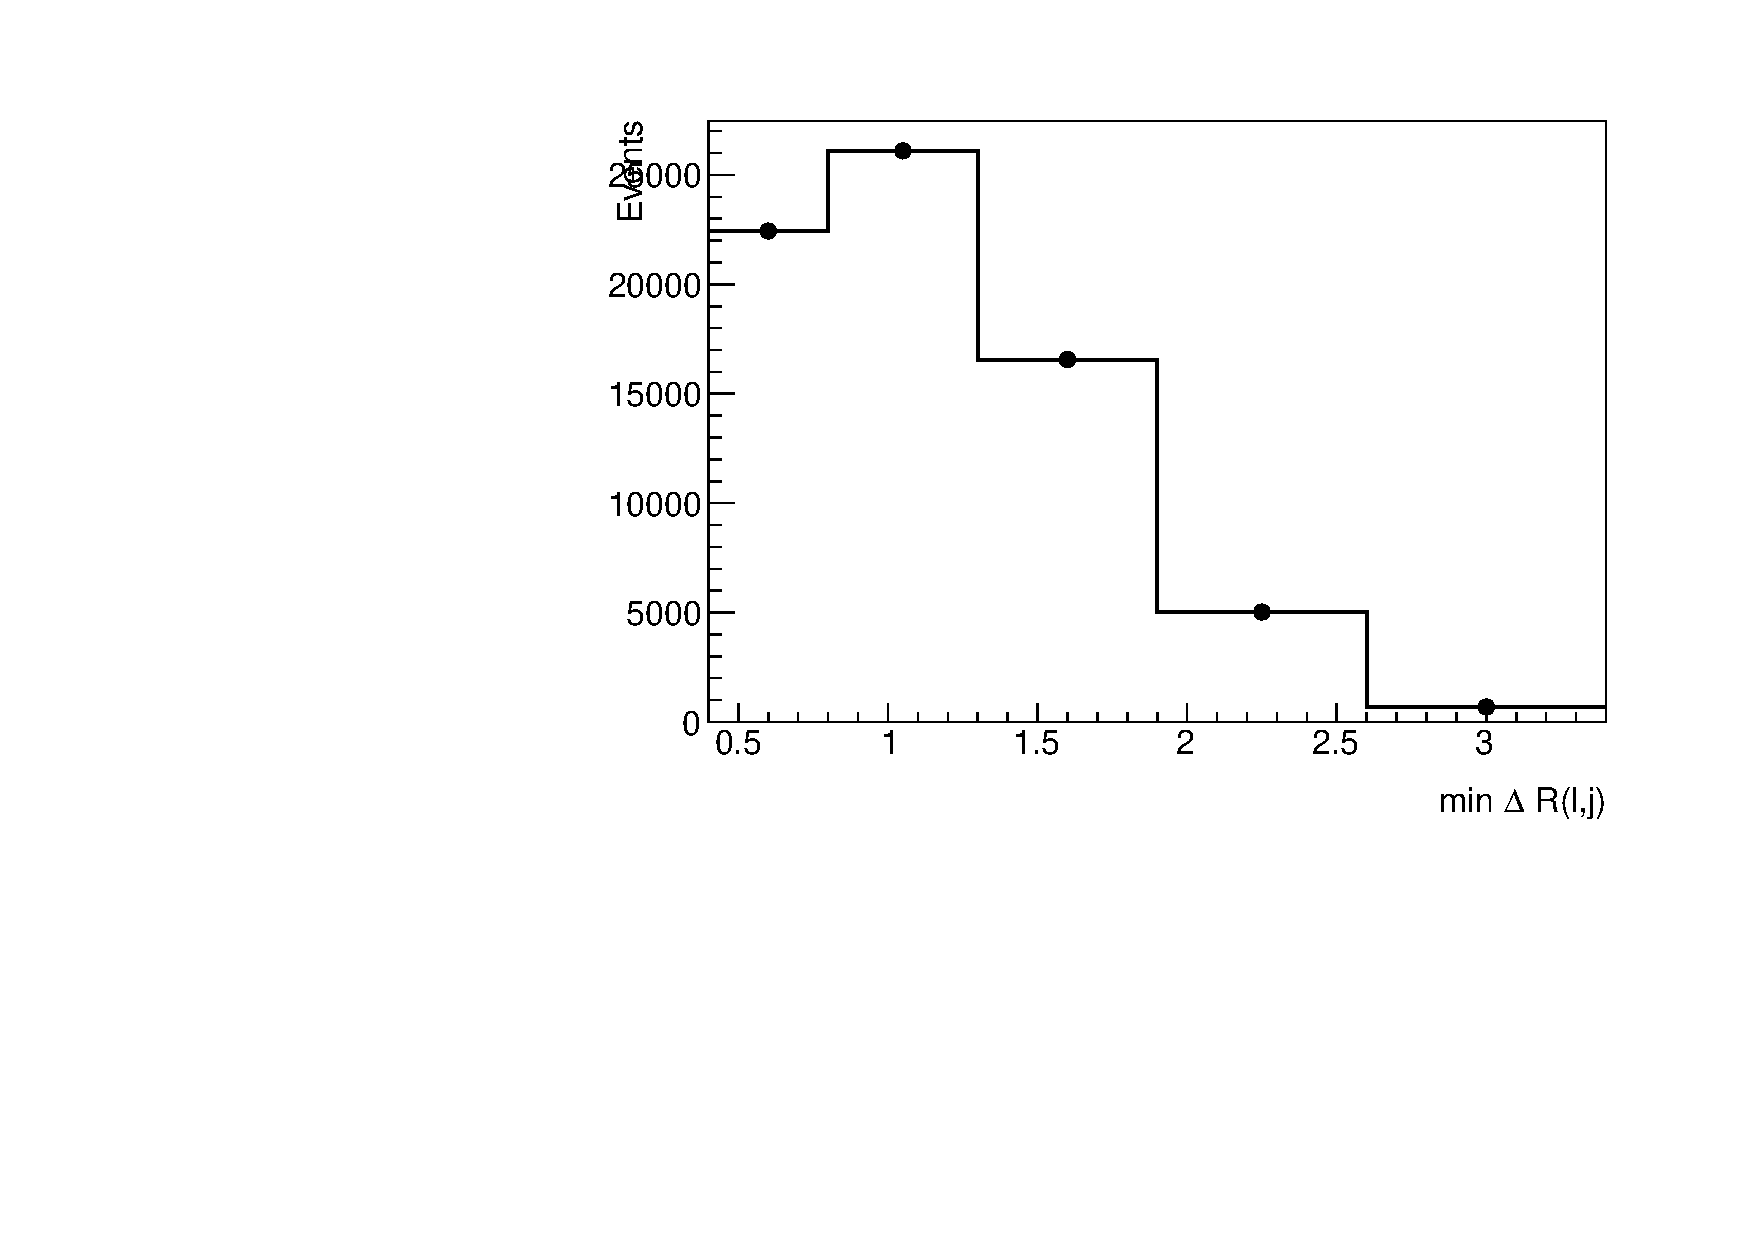
\includegraphics[width=0.3\textwidth]{figures/diff_xsec/ljet/Truth_dist/tty1l_drlj_all_syst_Unfolding_truth_distribution.pdf}}
    % pt j1
    \subfloat[]{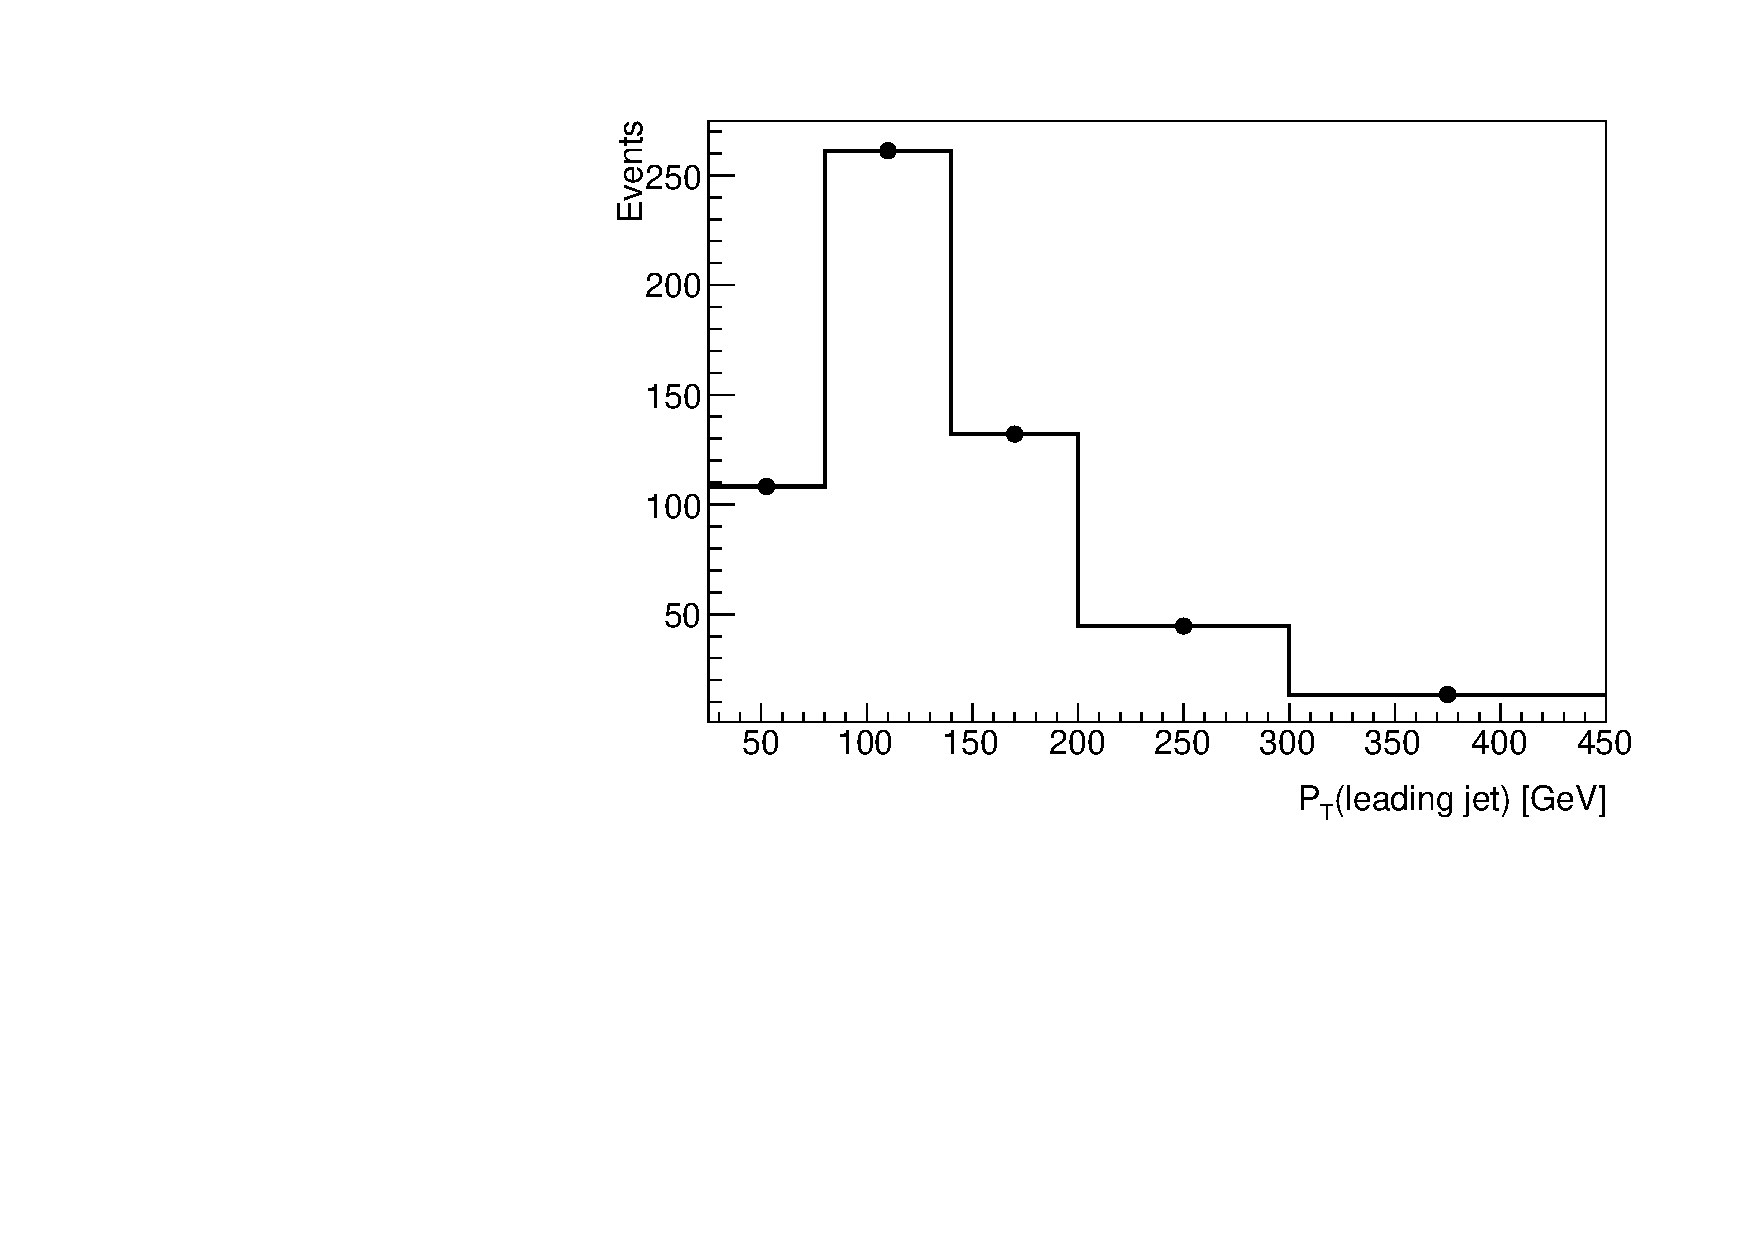
\includegraphics[width=0.3\textwidth]{figures/diff_xsec/ljet/Truth_dist/tty1l_ptj1_all_syst_Unfolding_truth_distribution.pdf}}
    \caption{The particle level distribution of \tty production as a function of different observables in the single-lepton channel. The number of events corresponds to the expected number of events at the particle level normalized to the luminosity of data. Overflow events are included in the last bin of the corresponding distribution. Note that values are divided by bin width.}
    \label{fig:folding_input_ljet}
\end{figure}
\FloatBarrier

\begin{figure}[ht]
    \centering
    % ph pt
    \subfloat[]{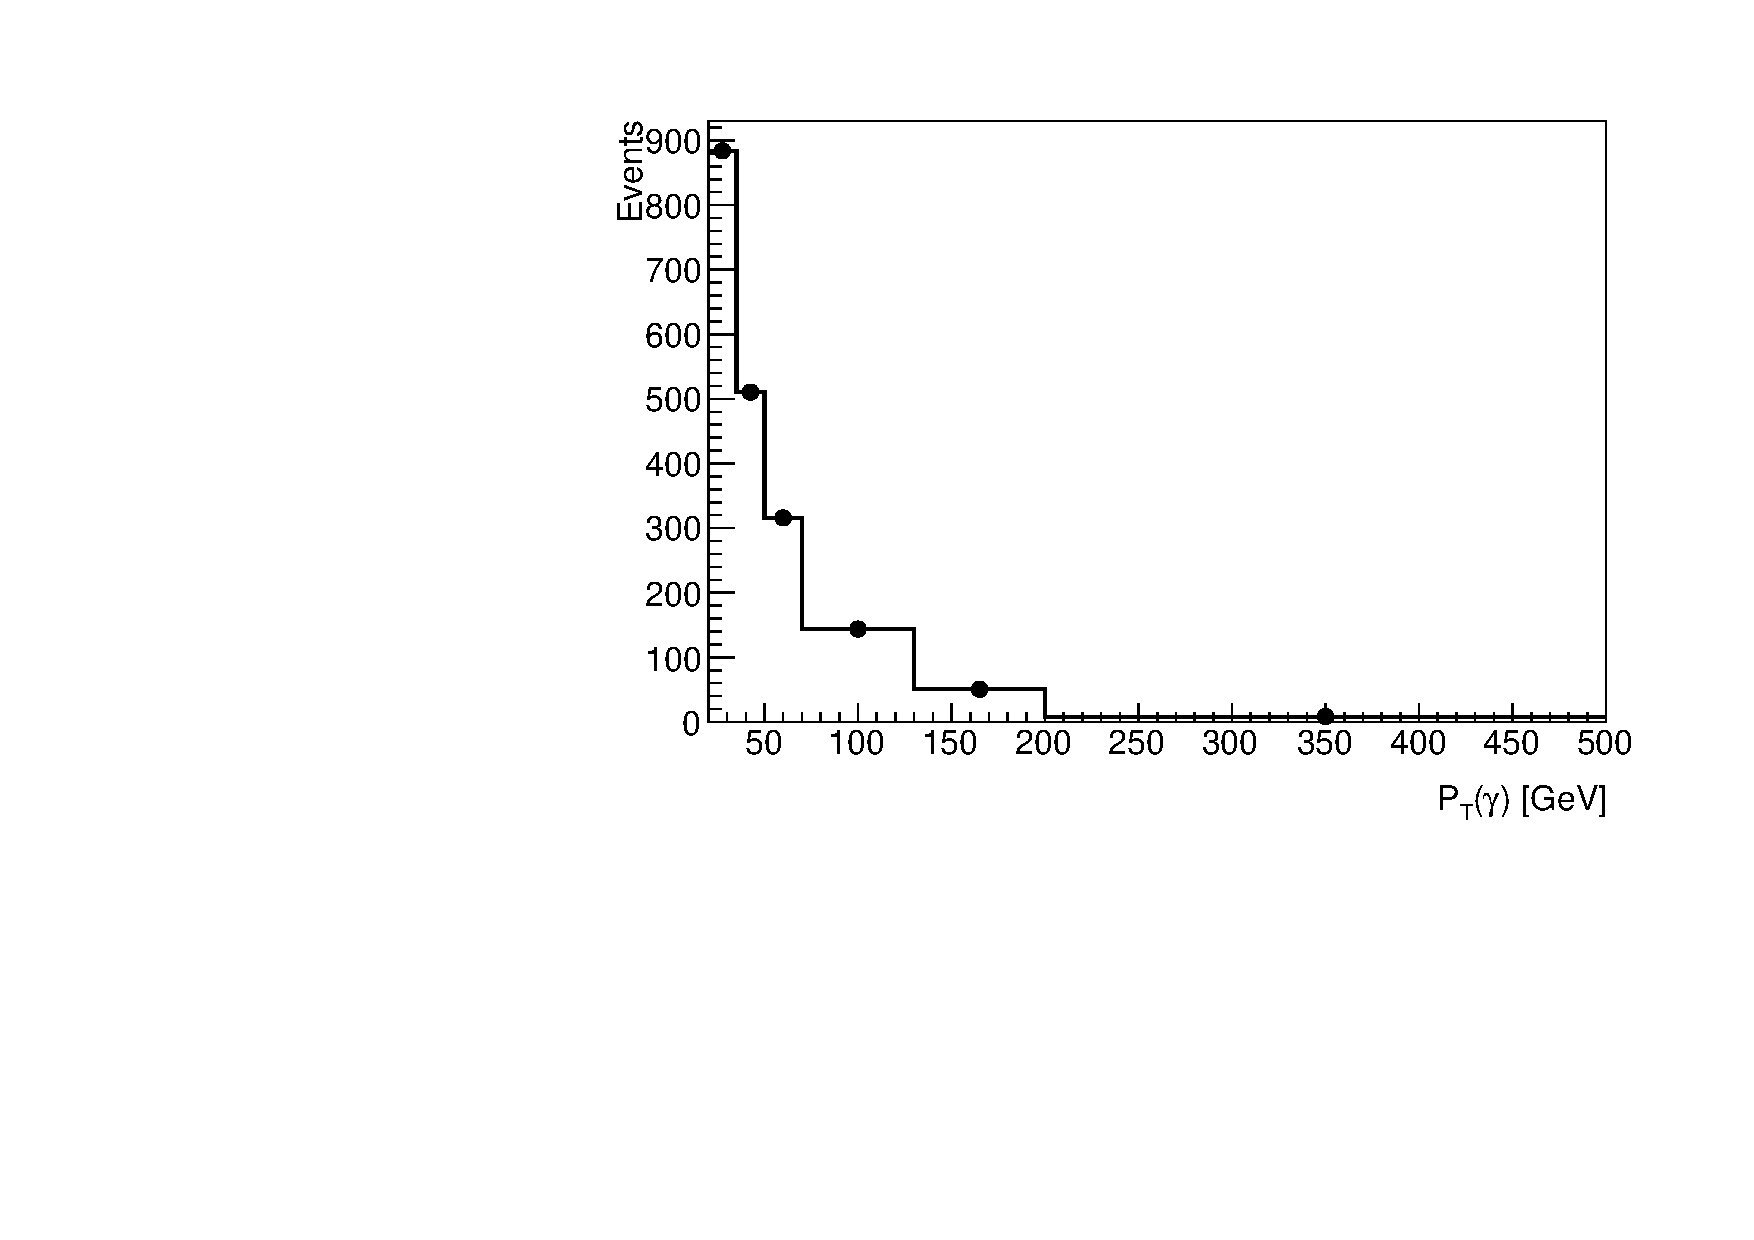
\includegraphics[width=0.3\textwidth]{figures/diff_xsec/dilep/Truth_dist/tty2l_pt_all_syst_Unfolding_truth_distribution.pdf}}
    \quad
    % ph eta
    \subfloat[]{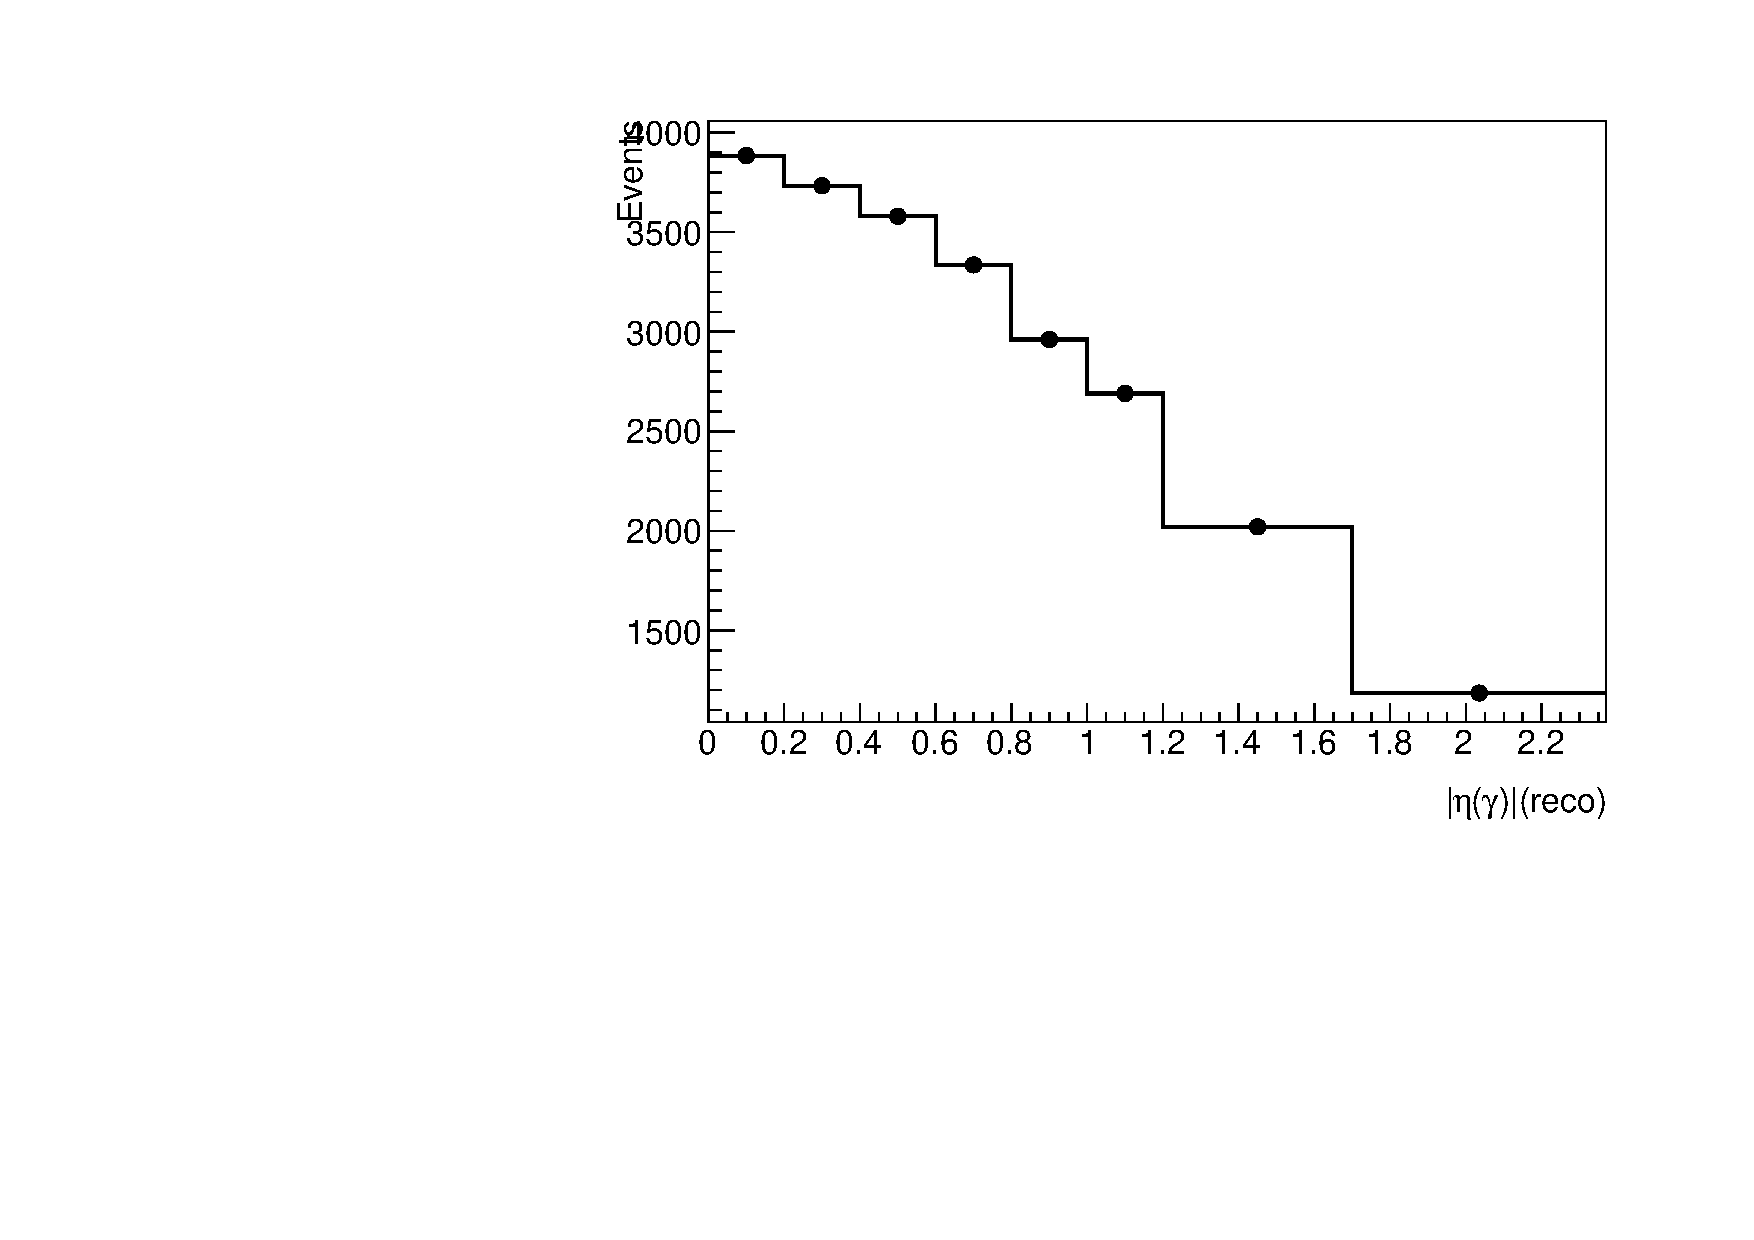
\includegraphics[width=0.3\textwidth]{figures/diff_xsec/dilep/Truth_dist/tty2l_eta_all_syst_Unfolding_truth_distribution.pdf}}
    \quad
    % delta R (ph, l)
    \subfloat[]{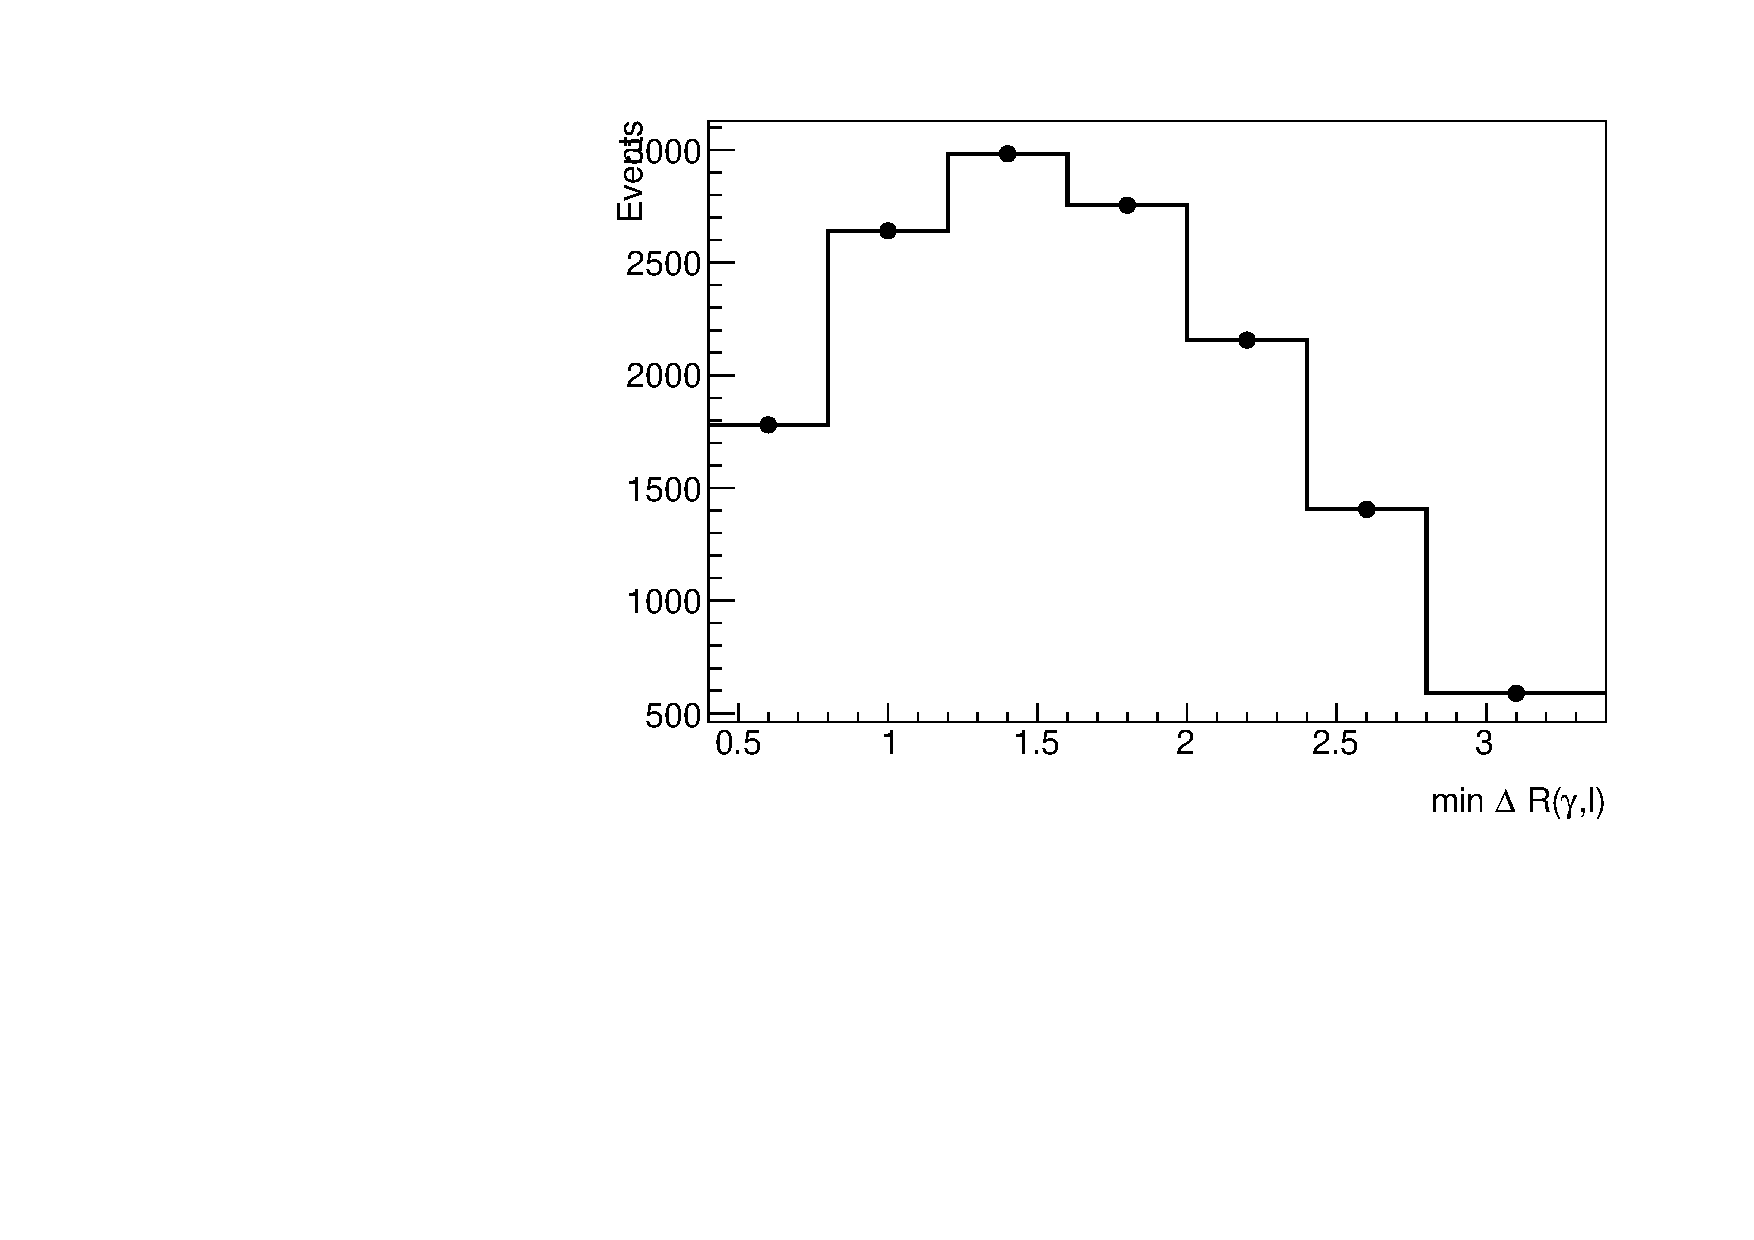
\includegraphics[width=0.3\textwidth]{figures/diff_xsec/dilep/Truth_dist/tty2l_dr_all_syst_Unfolding_truth_distribution.pdf}}
    \quad
    % delta R (ph, l1)
    \subfloat[]{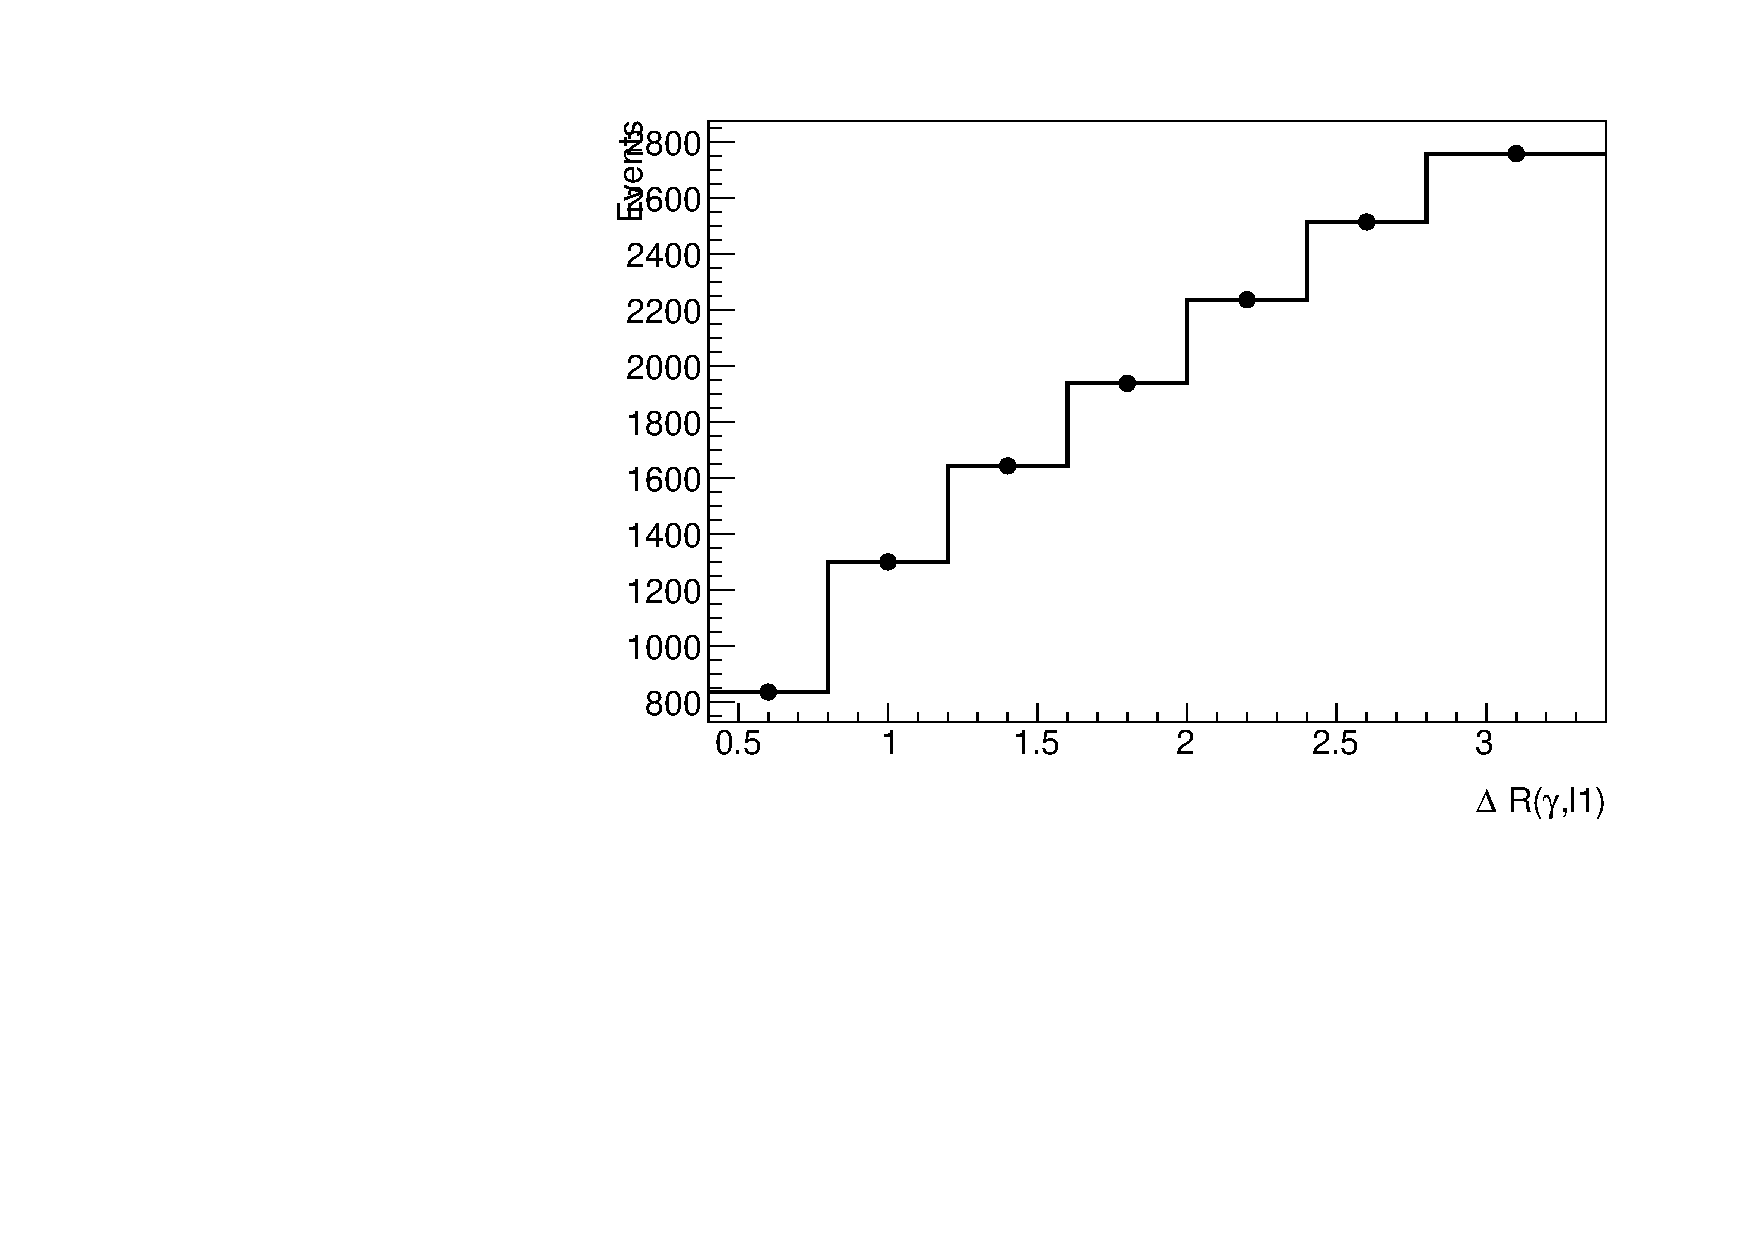
\includegraphics[width=0.3\textwidth]{figures/diff_xsec/dilep/Truth_dist/tty2l_dr1_all_syst_Unfolding_truth_distribution.pdf}}
    \quad
    % delta R (ph, l2)
    \subfloat[]{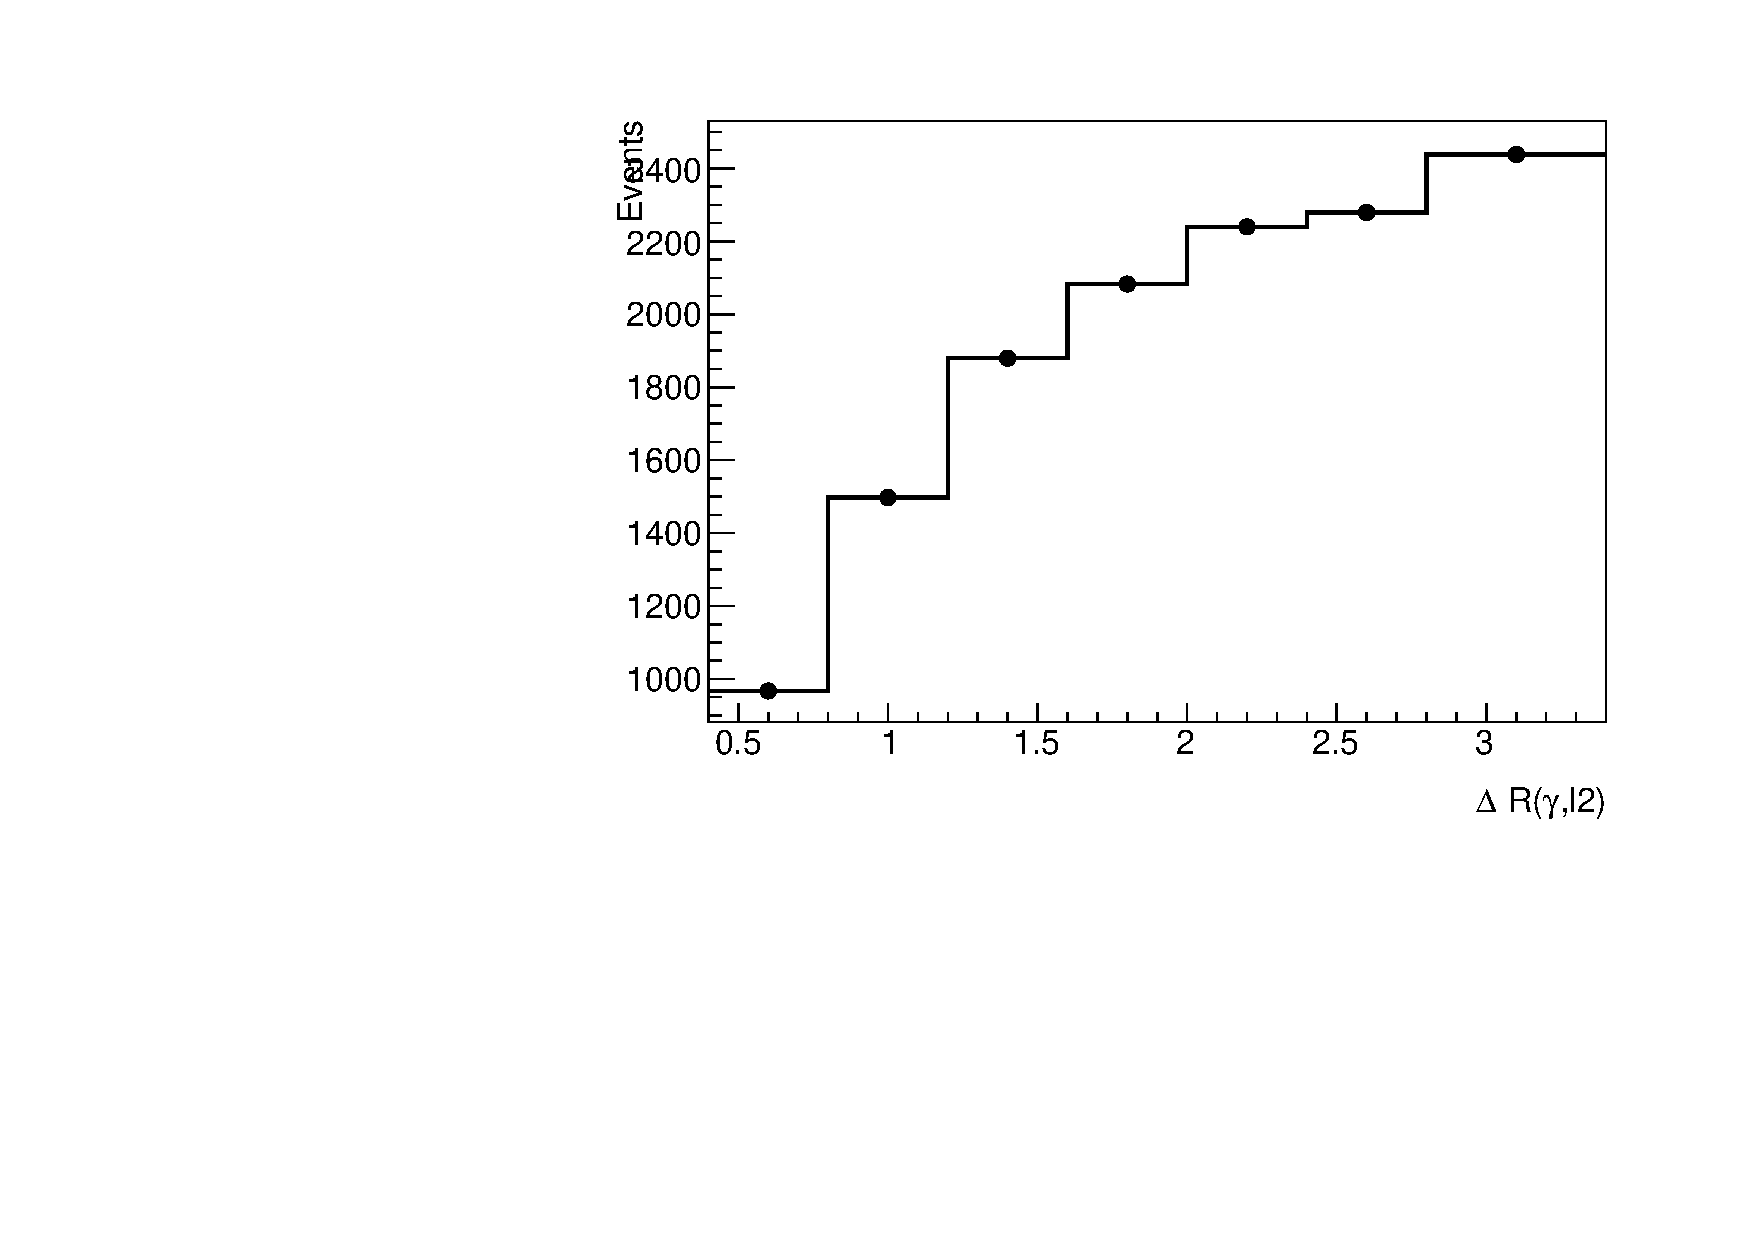
\includegraphics[width=0.3\textwidth]{figures/diff_xsec/dilep/Truth_dist/tty2l_dr2_all_syst_Unfolding_truth_distribution.pdf}}
    \quad
    % delta R (ph, b)
    \subfloat[]{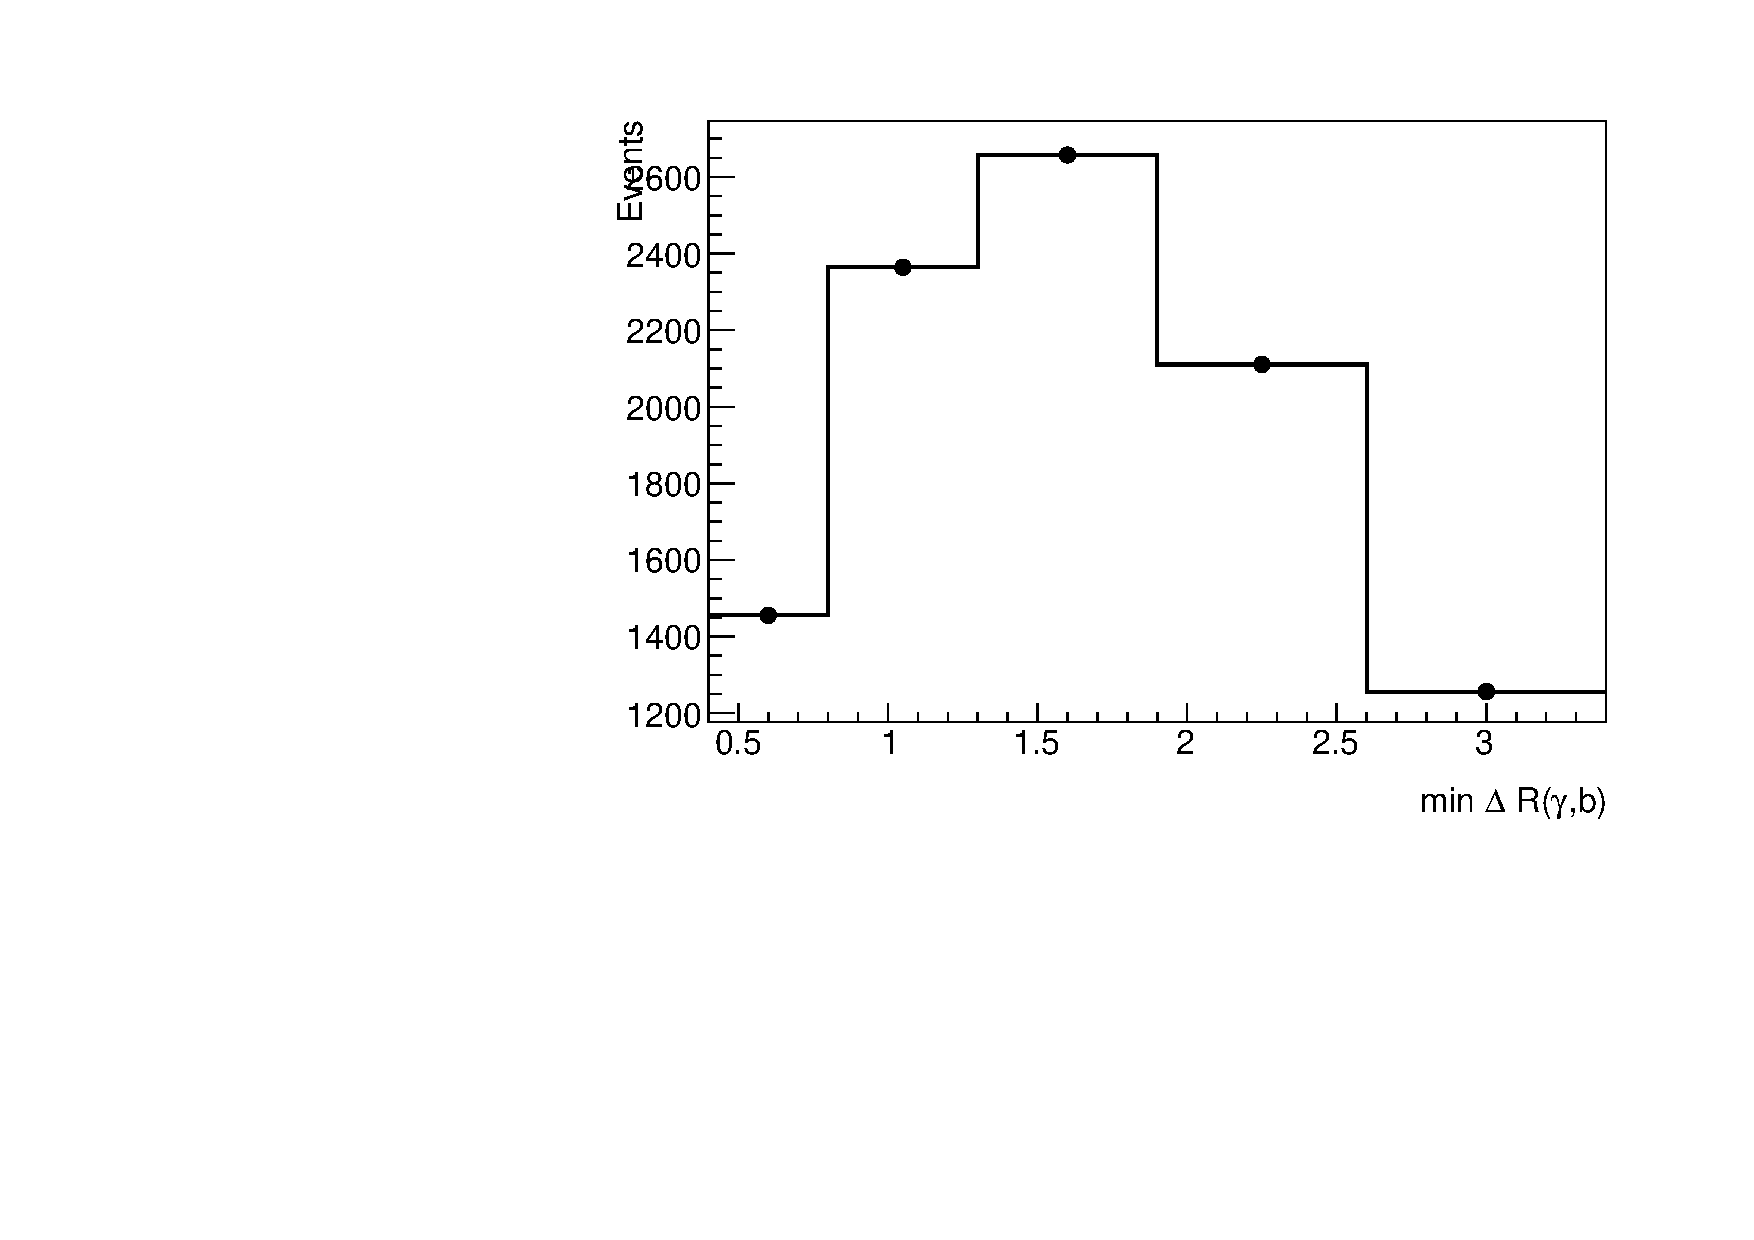
\includegraphics[width=0.3\textwidth]{figures/diff_xsec/dilep/Truth_dist/tty2l_drphb_all_syst_Unfolding_truth_distribution.pdf}}
    \quad
    % dEta(ll)
    \subfloat[]{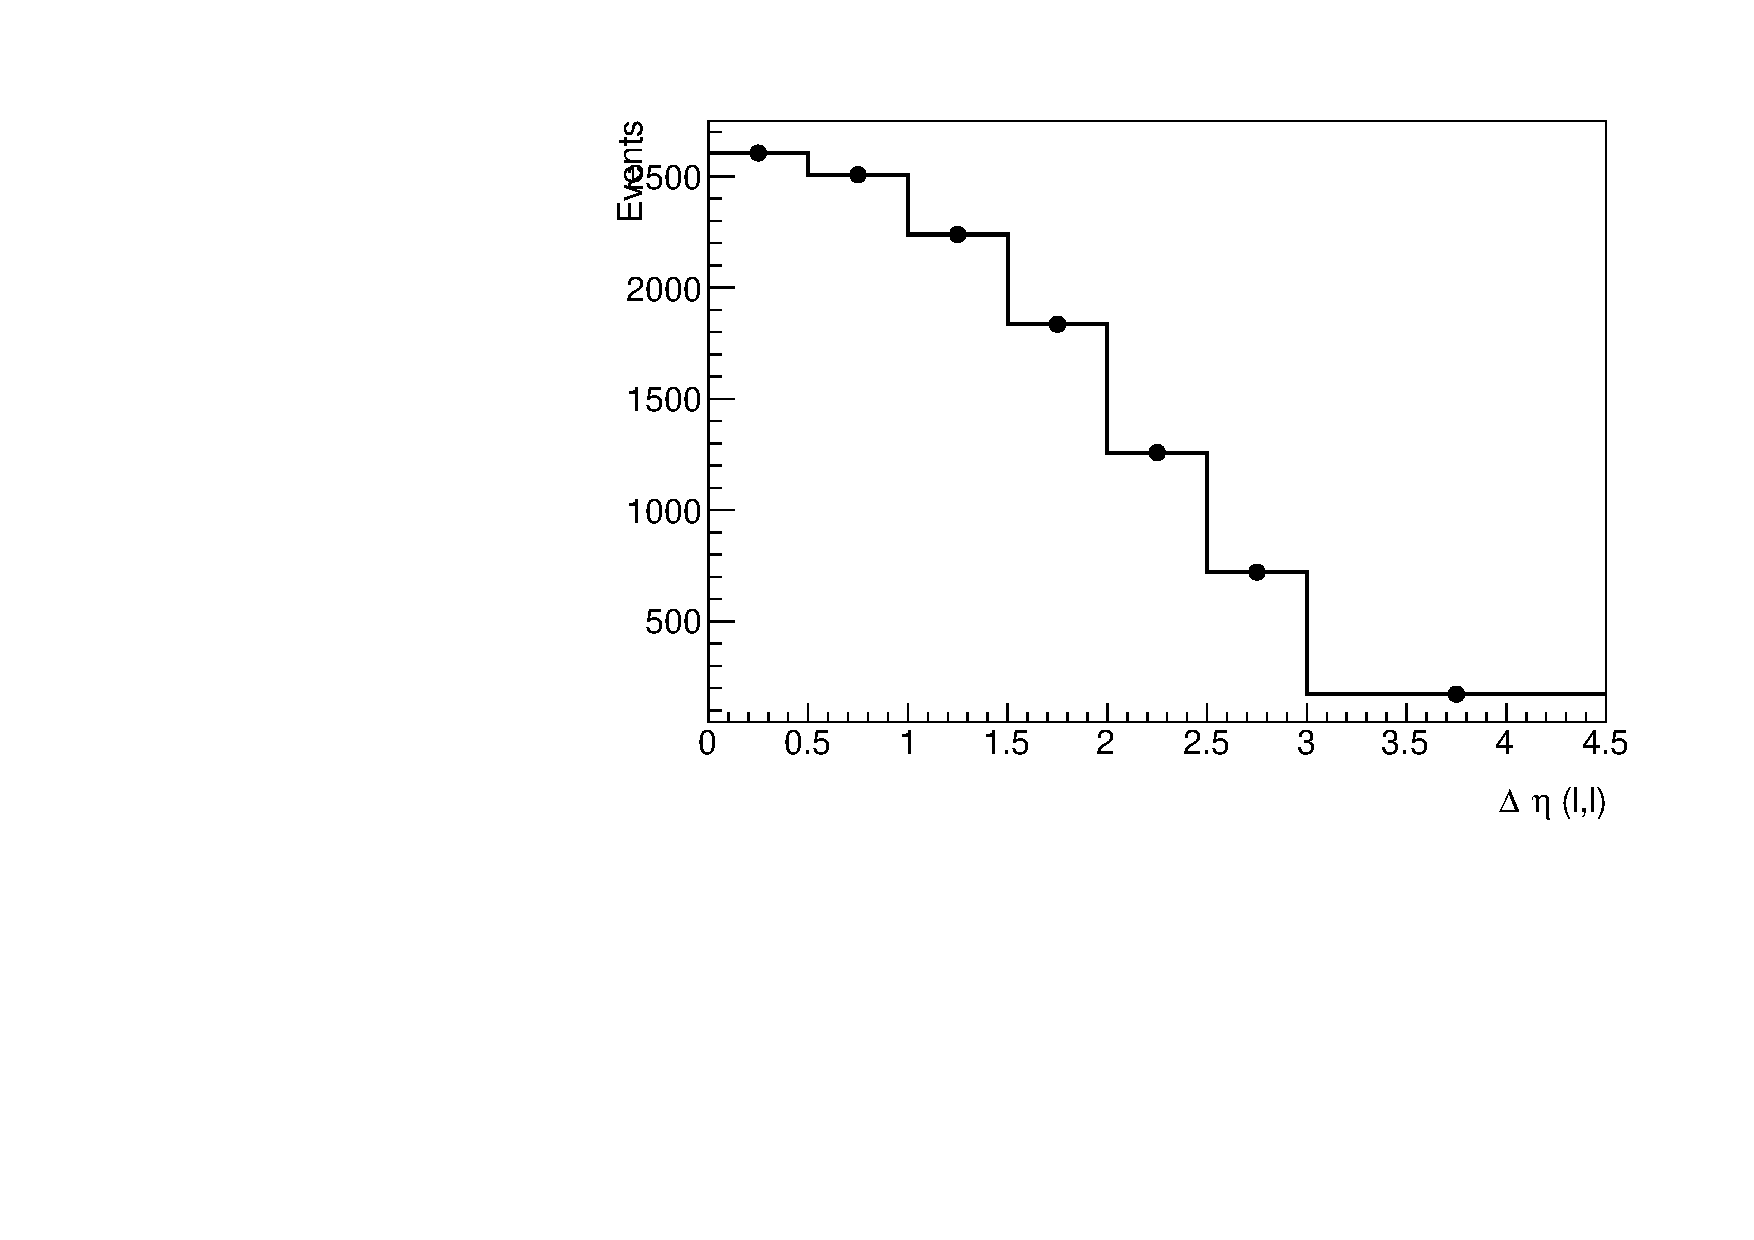
\includegraphics[width=0.3\textwidth]{figures/diff_xsec/dilep/Truth_dist/tty2l_dEtall_all_syst_Unfolding_truth_distribution.pdf}}
    \quad
    % dPhi(ll)
    \subfloat[]{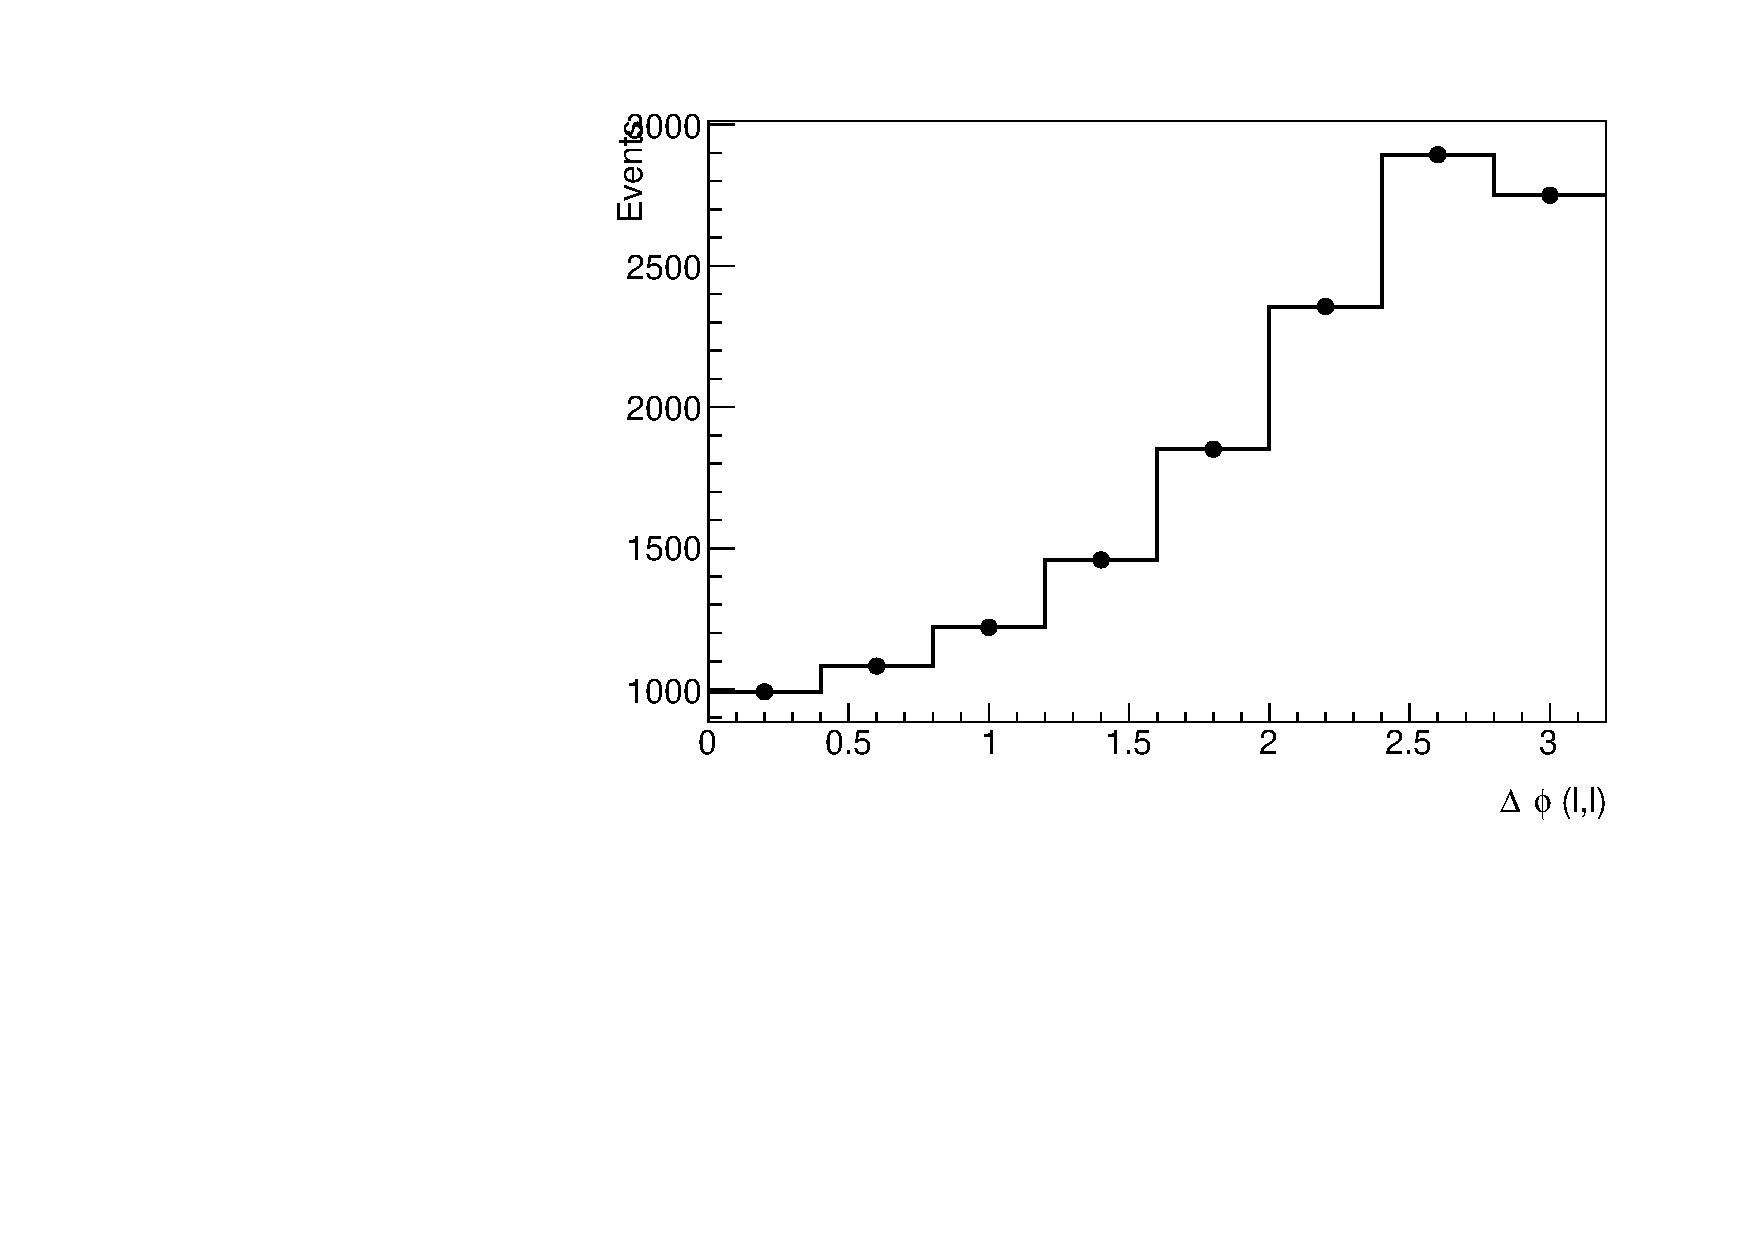
\includegraphics[width=0.3\textwidth]{figures/diff_xsec/dilep/Truth_dist/tty2l_dPhill_all_syst_Unfolding_truth_distribution.pdf}}
    \quad
    % Pt(ll)
    \subfloat[]{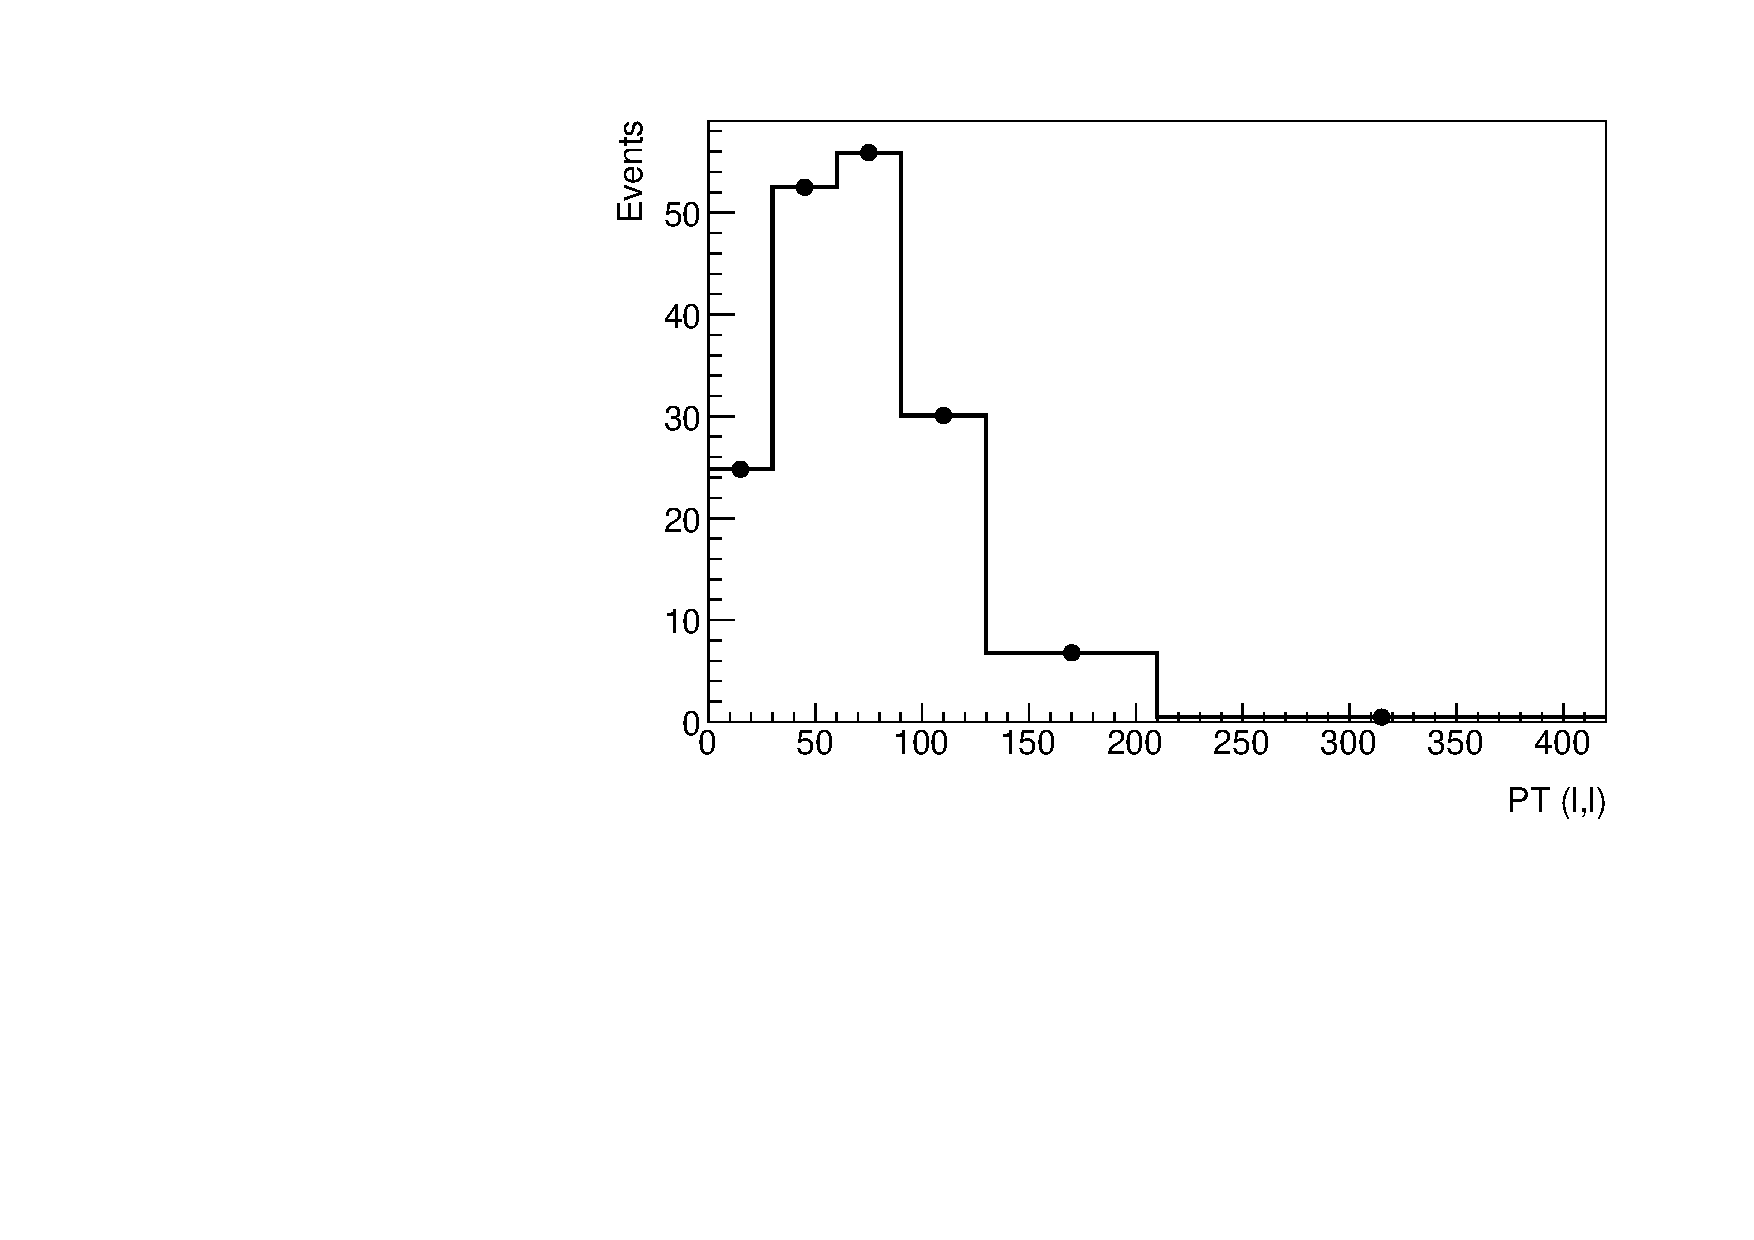
\includegraphics[width=0.3\textwidth]{figures/diff_xsec/dilep/Truth_dist/tty2l_ptll_all_syst_Unfolding_truth_distribution.pdf}}
    \quad
    % Delta R (lj)
    \subfloat[]{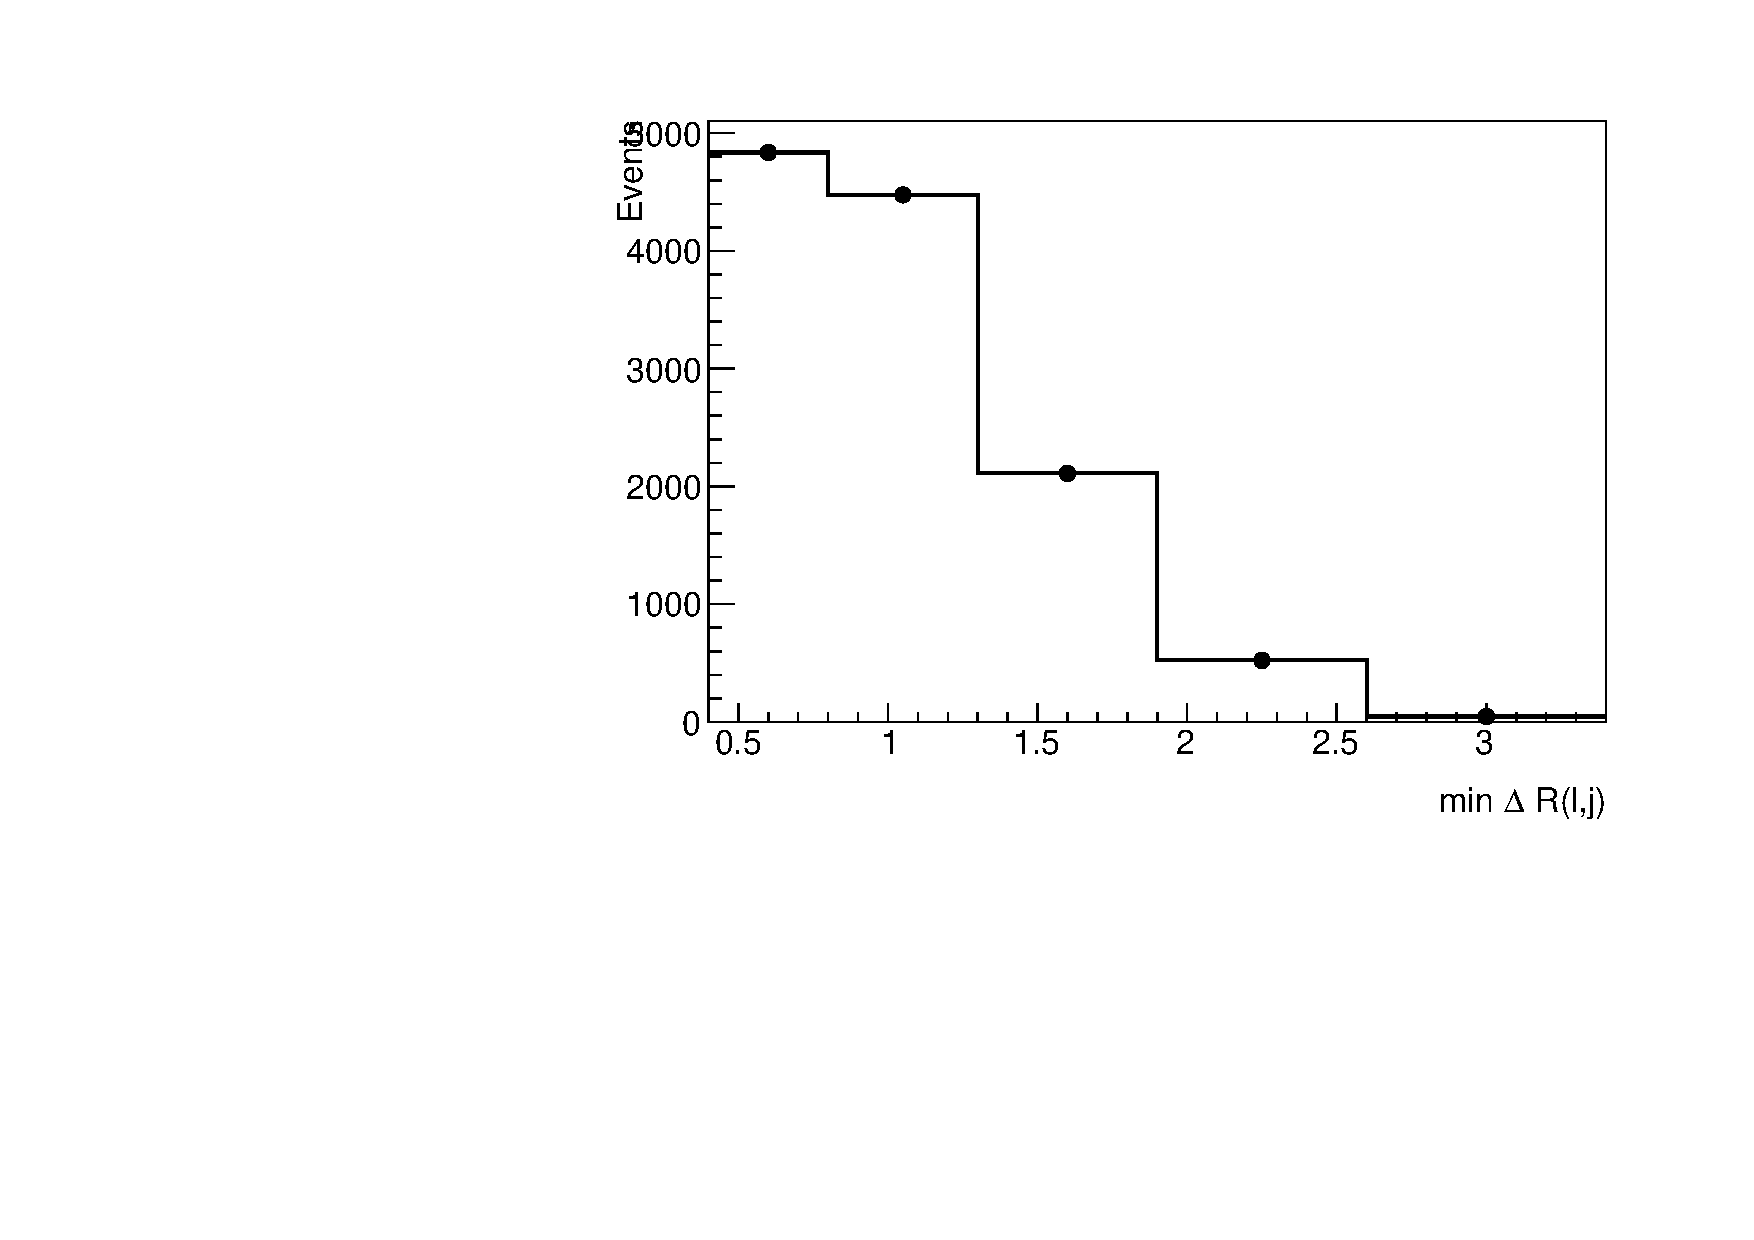
\includegraphics[width=0.3\textwidth]{figures/diff_xsec/dilep/Truth_dist/tty2l_drlj_all_syst_Unfolding_truth_distribution.pdf}}
    \quad
    % pt j1
    \subfloat[]{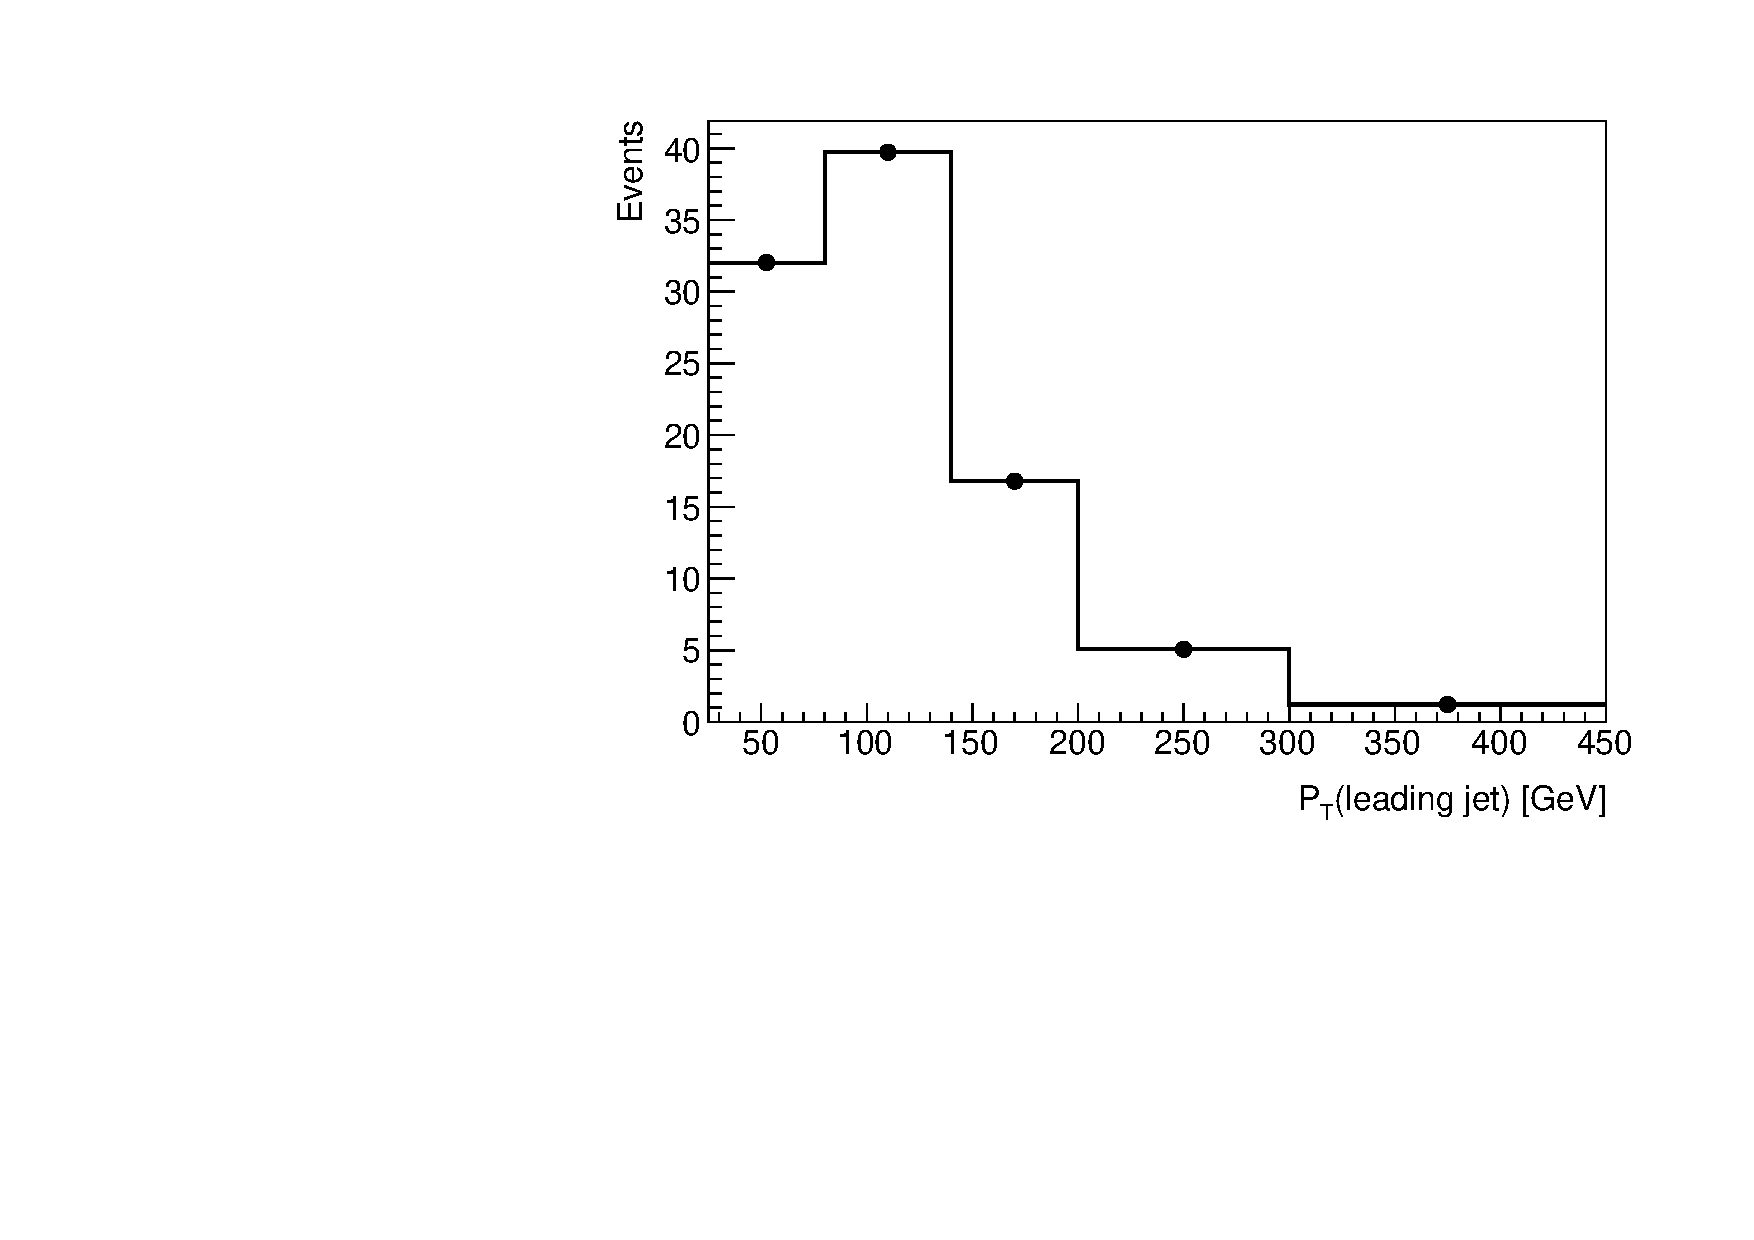
\includegraphics[width=0.3\textwidth]{figures/diff_xsec/dilep/Truth_dist/tty2l_ptj1_all_syst_Unfolding_truth_distribution.pdf}}

    \caption{The particle level distribution of \tty production as a function of different observables in the dilepton channel. The number of events corresponds to the expected number of events at the particle level normalized to the luminosity of data. Overflow events are included in the last bin of the corresponding distribution. Note that values are divided by bin width.}
    \label{fig:folding_input_dilep1}
\end{figure}
\FloatBarrier


%%%%%%%%
%  Migration matrices ljet 
%%%%%%%%
\begin{figure}[ht]
    \centering
    \subfloat[]{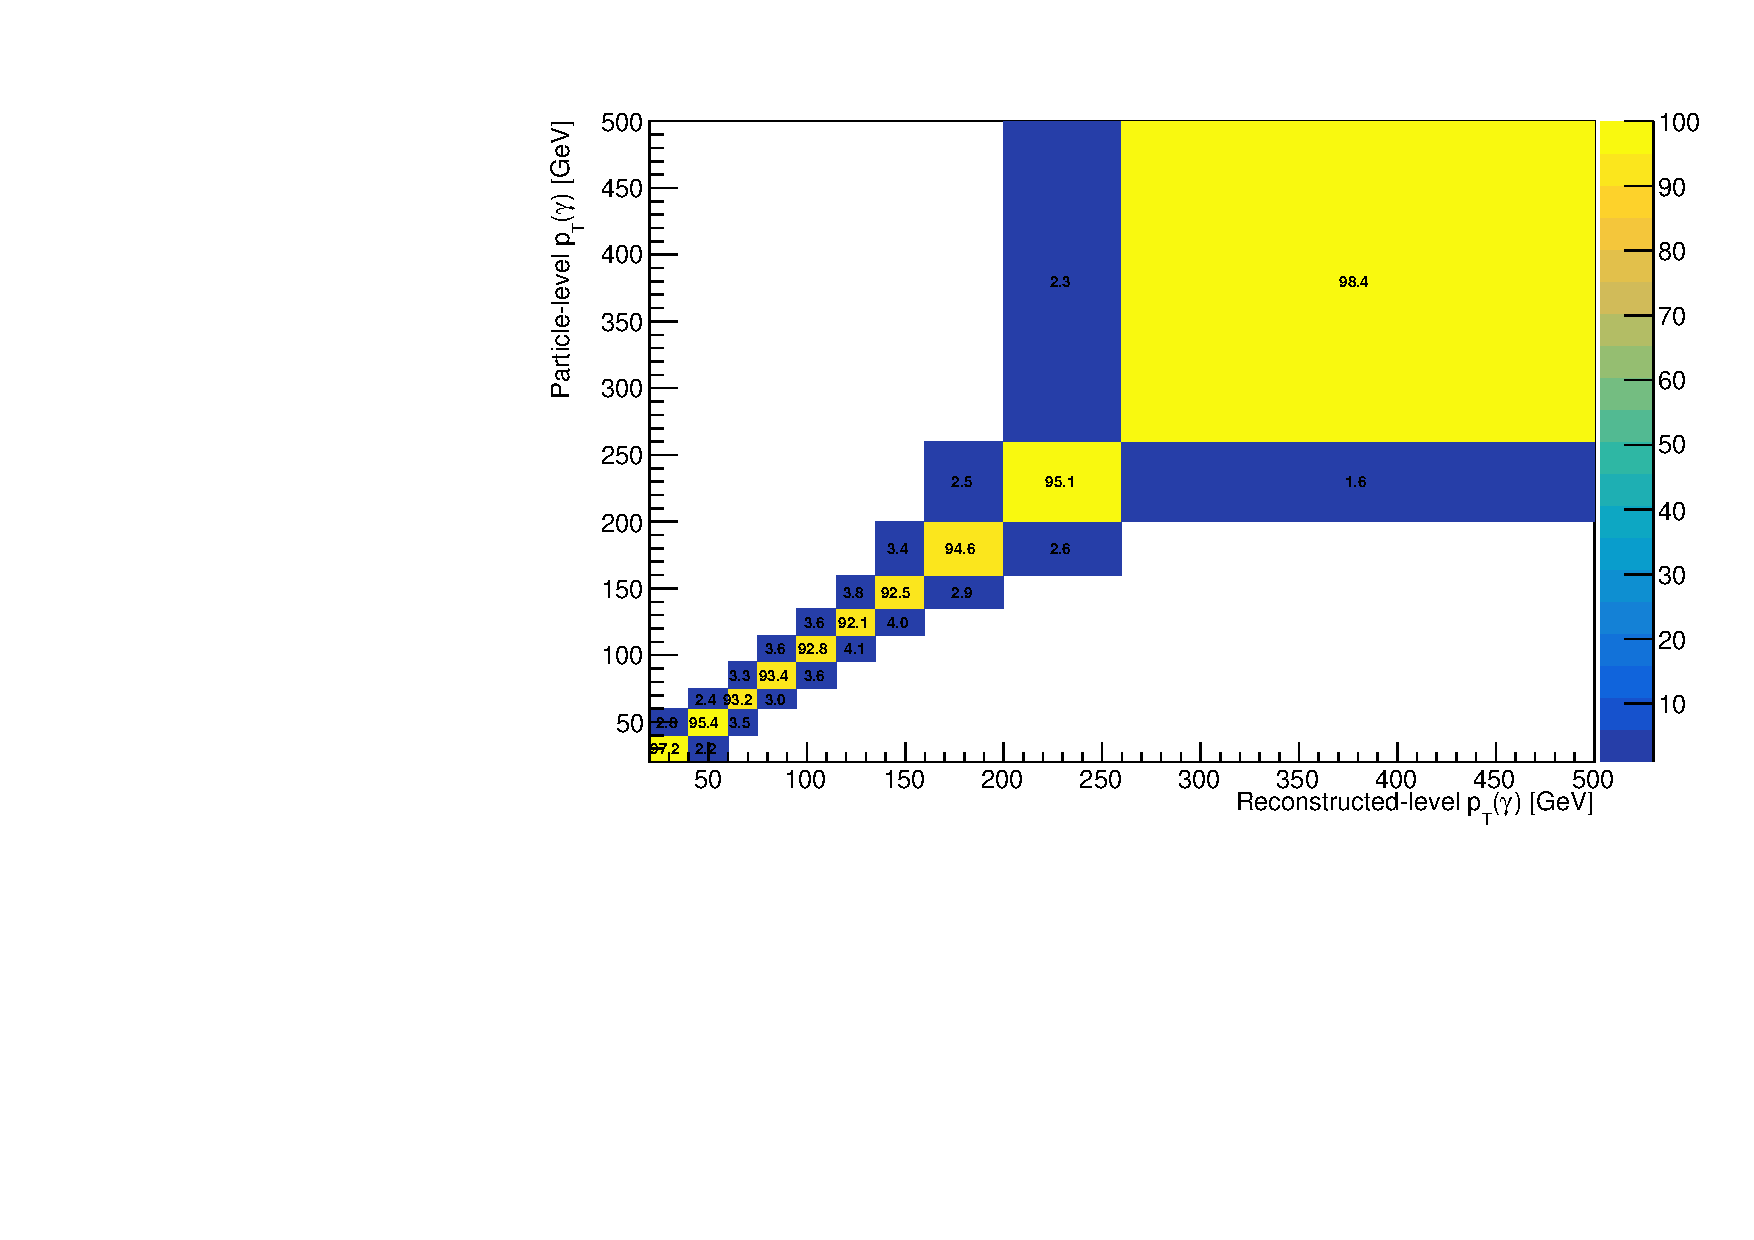
\includegraphics[width=0.3\textwidth]{figures/diff_xsec/ljet/Migration/migration_h2_ph_pt_reco_part_full_weighted_SR1.pdf}}
    \quad\quad
    \subfloat[]{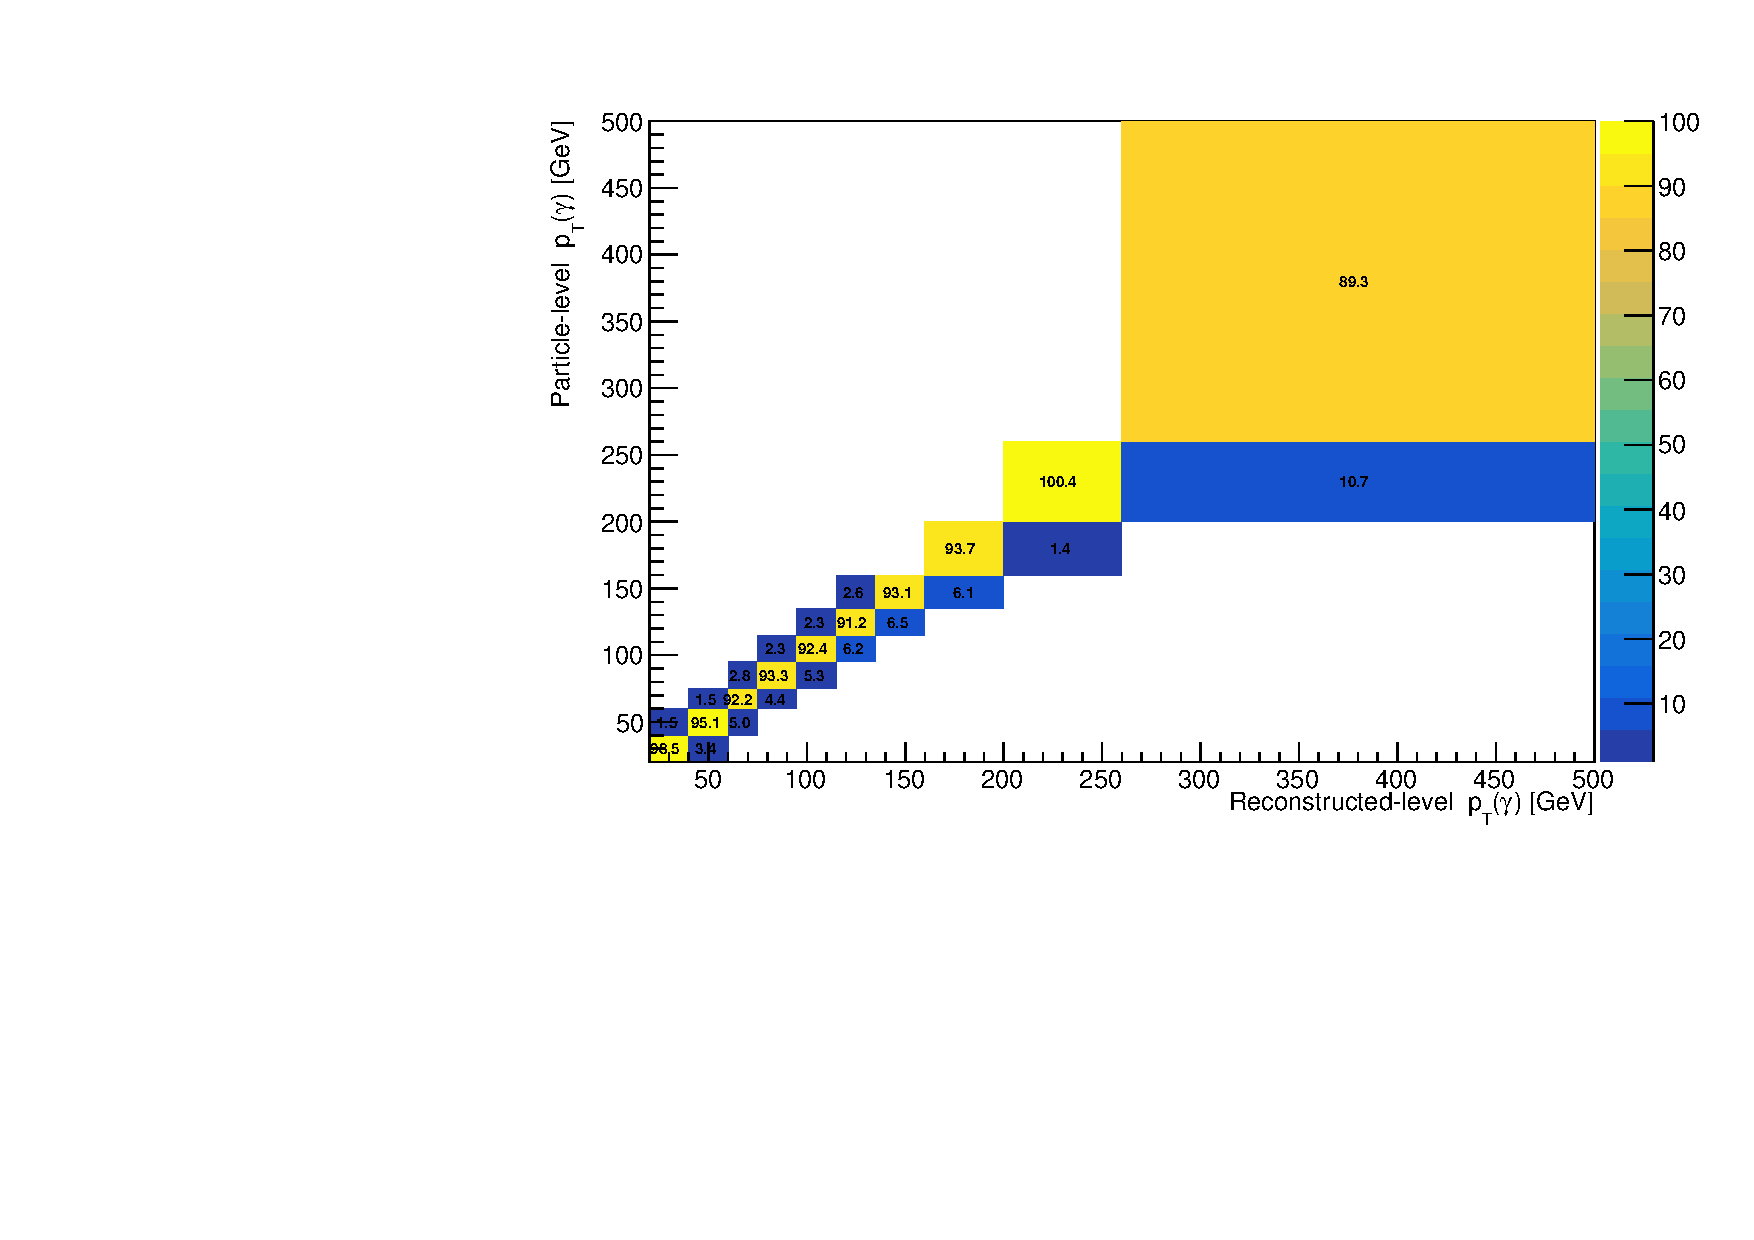
\includegraphics[width=0.3\textwidth]{figures/diff_xsec/ljet/Migration/migration_h2_ph_pt_reco_part_full_weighted_SR2.pdf}}
    \quad\quad
    \subfloat[]{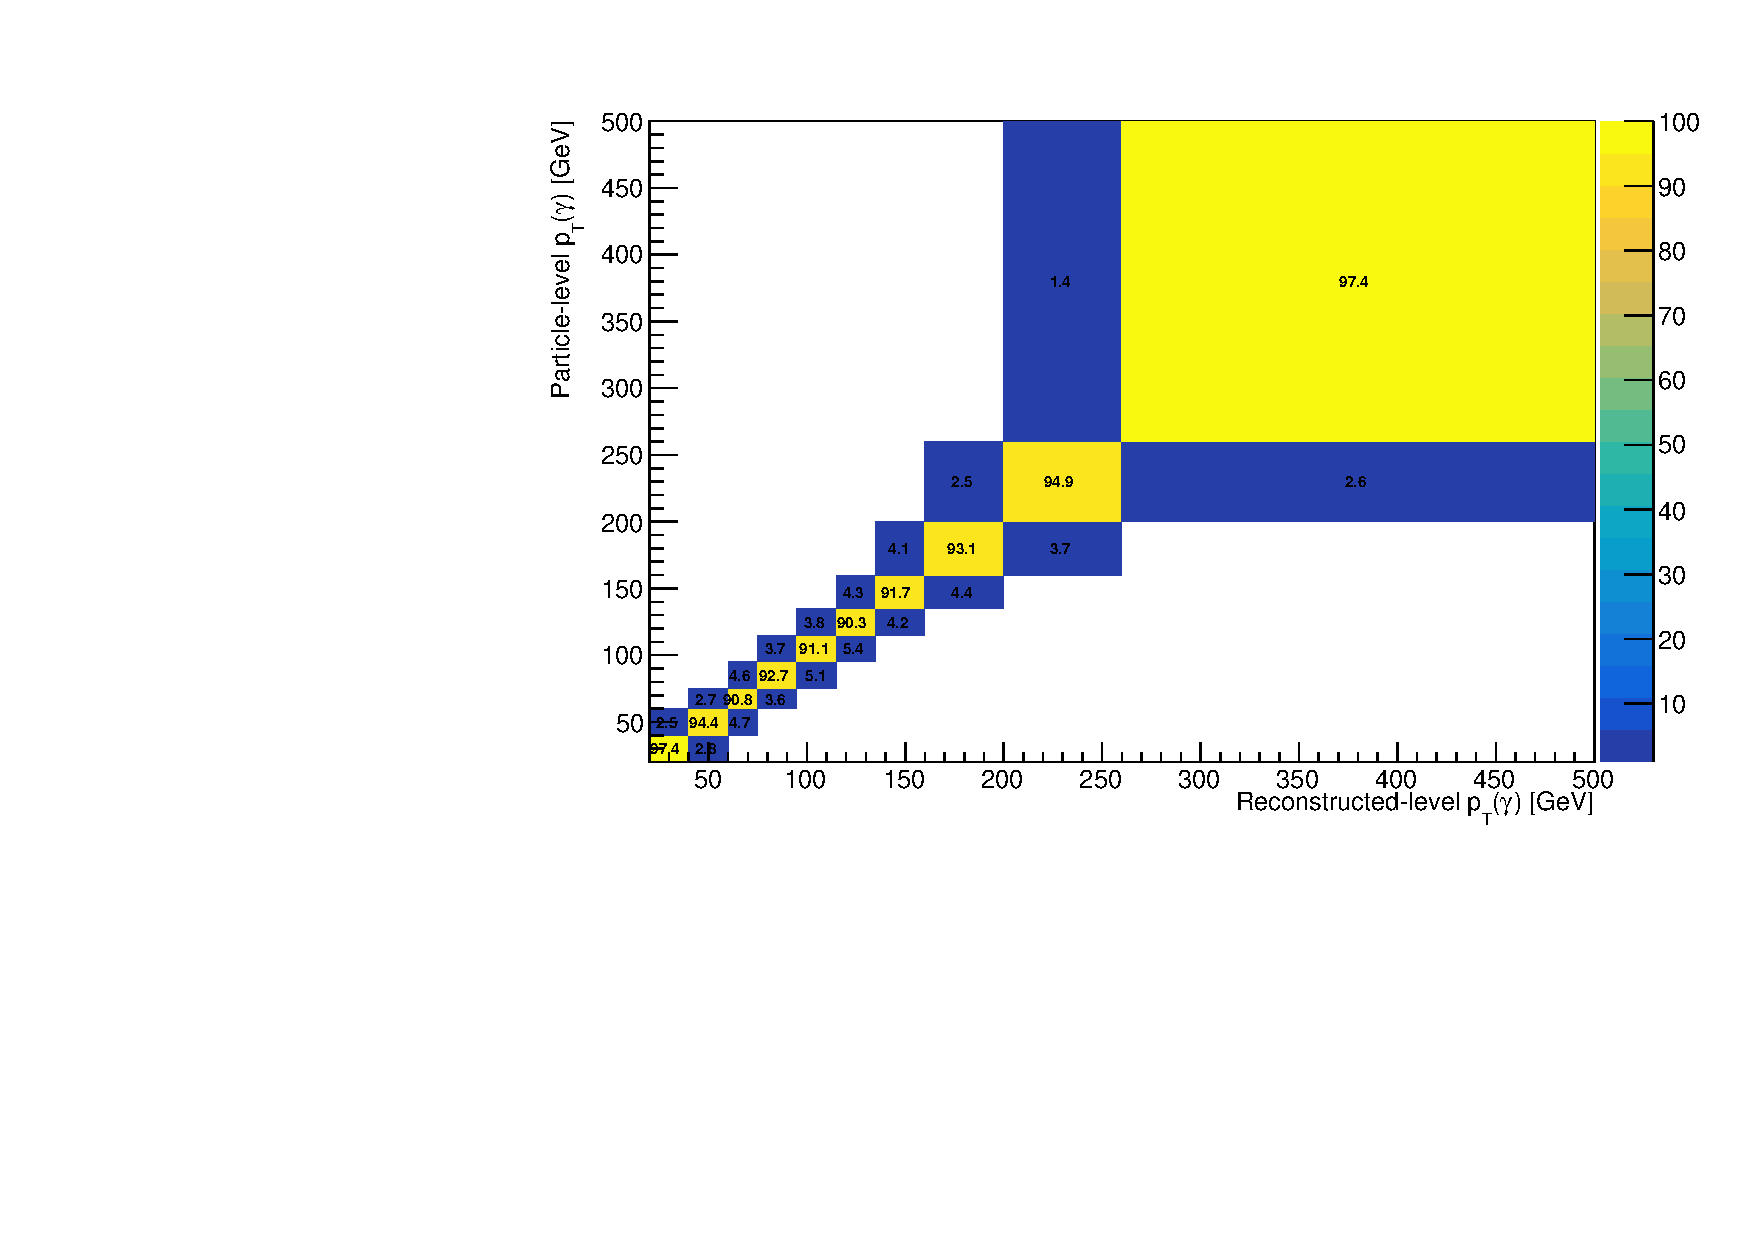
\includegraphics[width=0.3\textwidth]{figures/diff_xsec/ljet/Migration/migration_h2_ph_pt_reco_part_full_weighted_SR3.pdf}}
    \quad\quad
    \subfloat[]{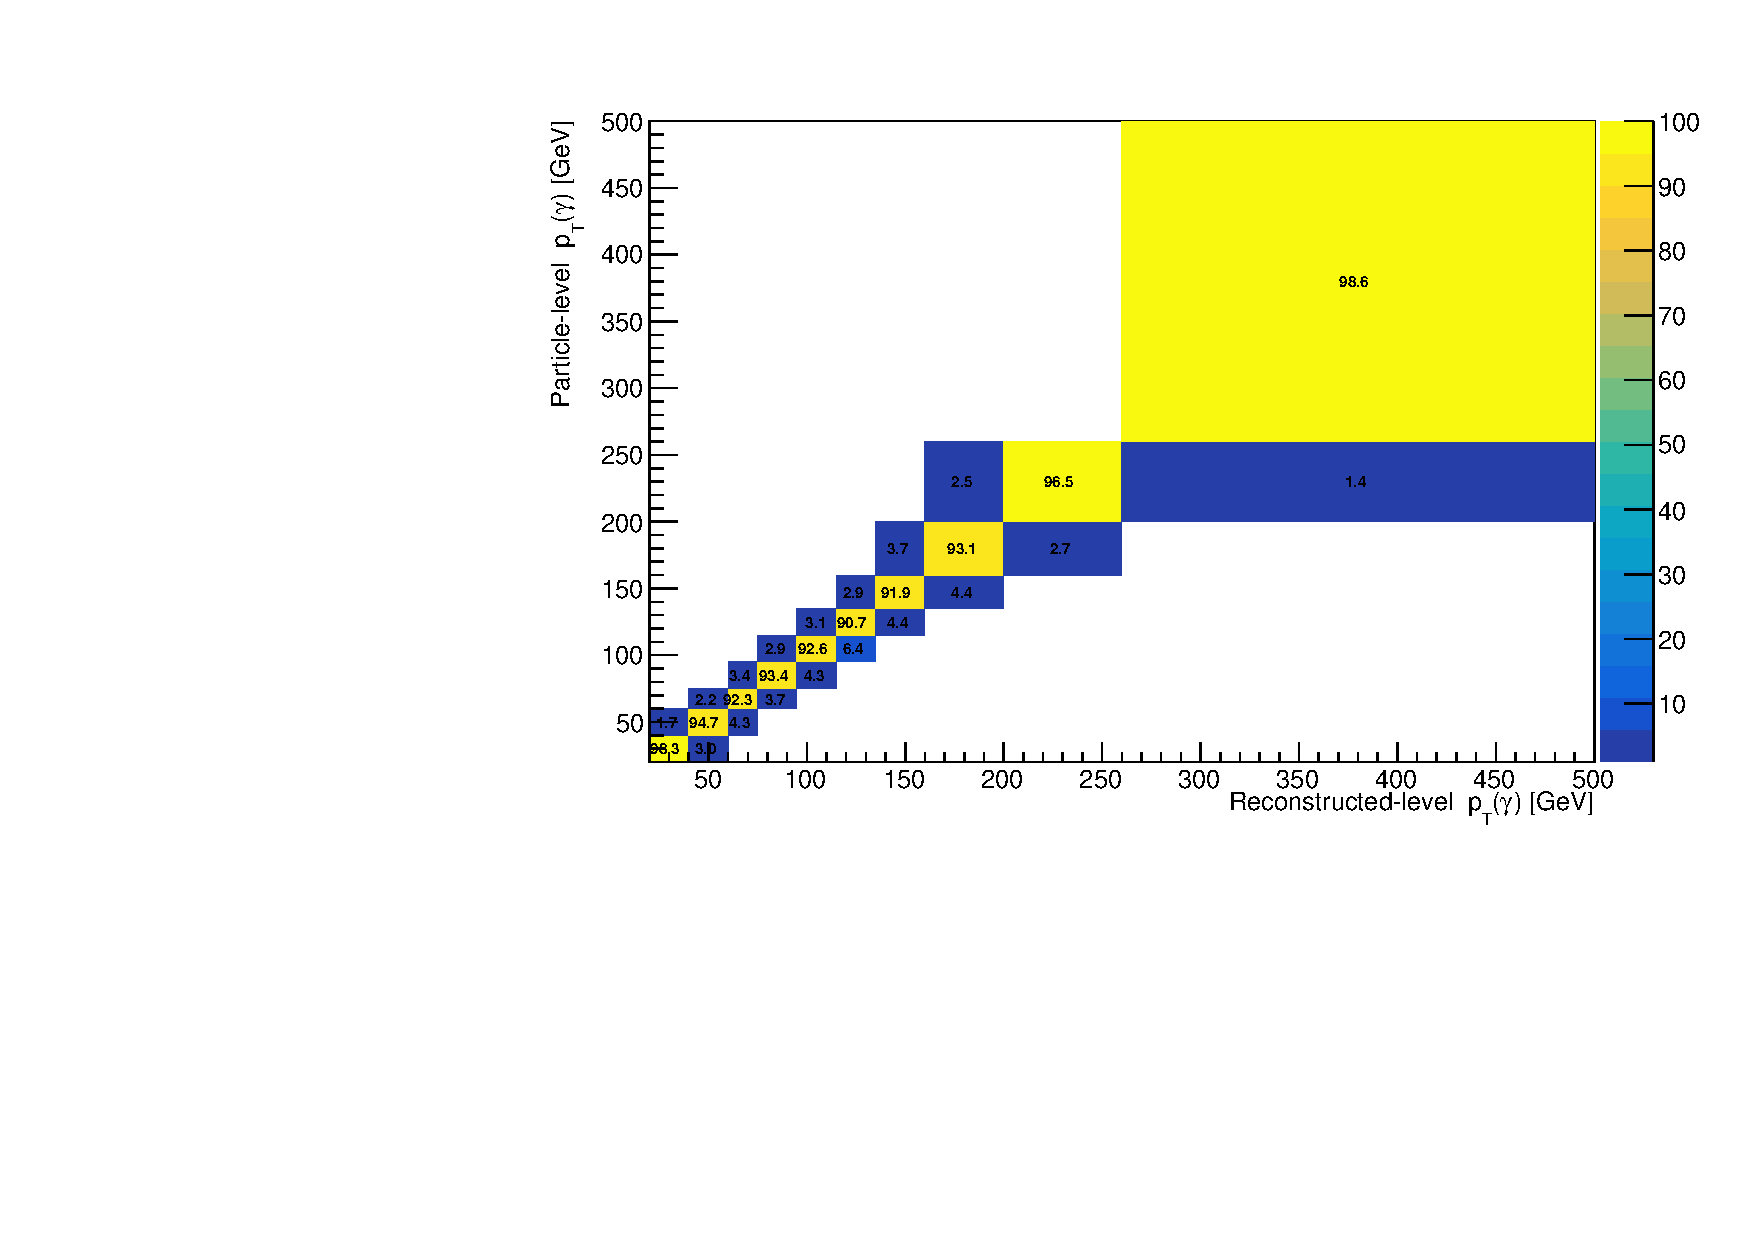
\includegraphics[width=0.3\textwidth]{figures/diff_xsec/ljet/Migration/migration_h2_ph_pt_reco_part_full_weighted_SR4.pdf}}
    \quad\quad
    \caption{The normalized migration matrices, $M_{\mathrm{r,t}}$, representing the migration of events from particle level to four regions at the reconstruction level: (a) \tty production enriched region, (b) \tty decay enriched region (c) fakes enriched region, (d) prompt photon enriched region for the observable $p_T(\gamma)$ in single-lepton channel.}
    \label{fig:folding_input_migration_ljet}
\end{figure}
\FloatBarrier

%%%%%%%%
%  Response matrices ljet
%%%
\begin{figure}[!ht]
  \centering
  \subfloat[]{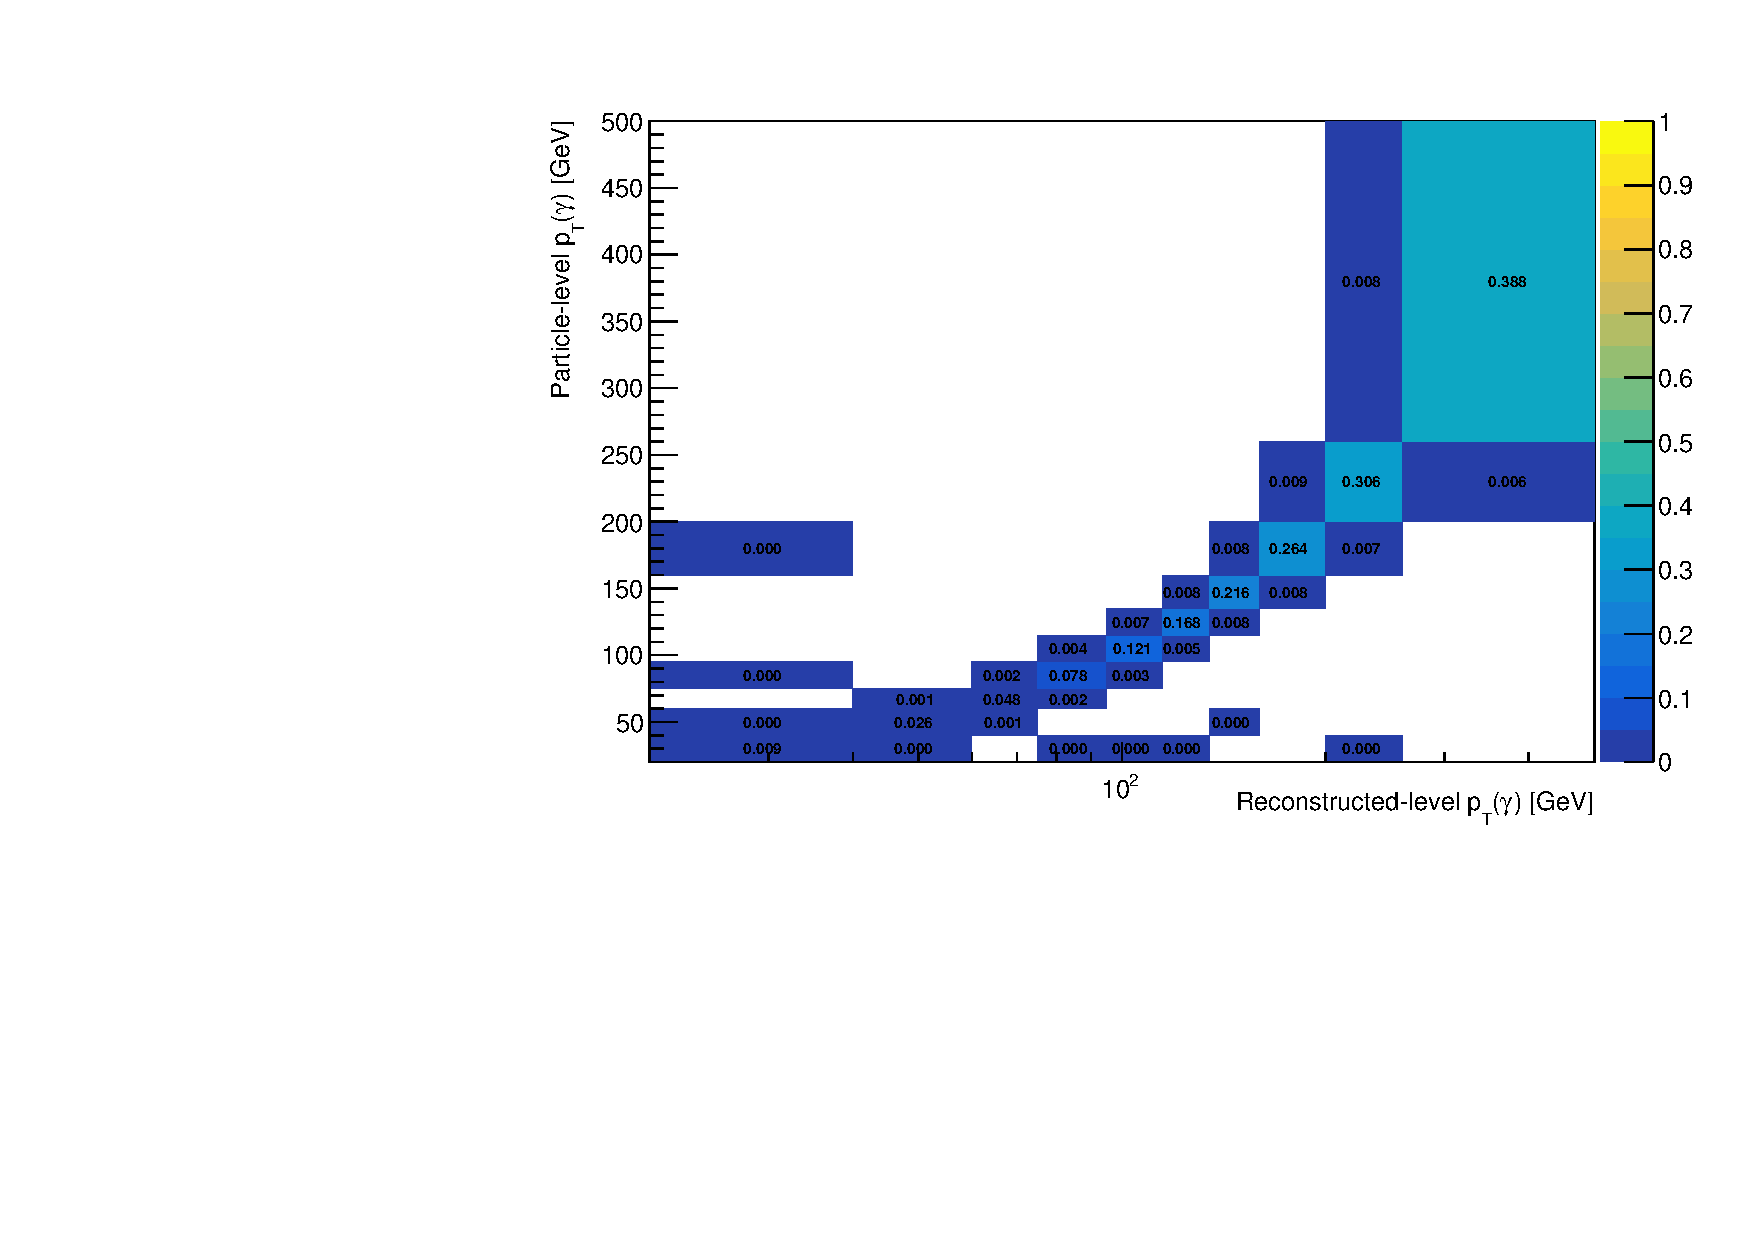
\includegraphics[width=0.3\textwidth]{figures/diff_xsec/ljet/Migration/response_h2_response_matrix_ph_pt_SR1.pdf}}
  \quad\quad
  \subfloat[]{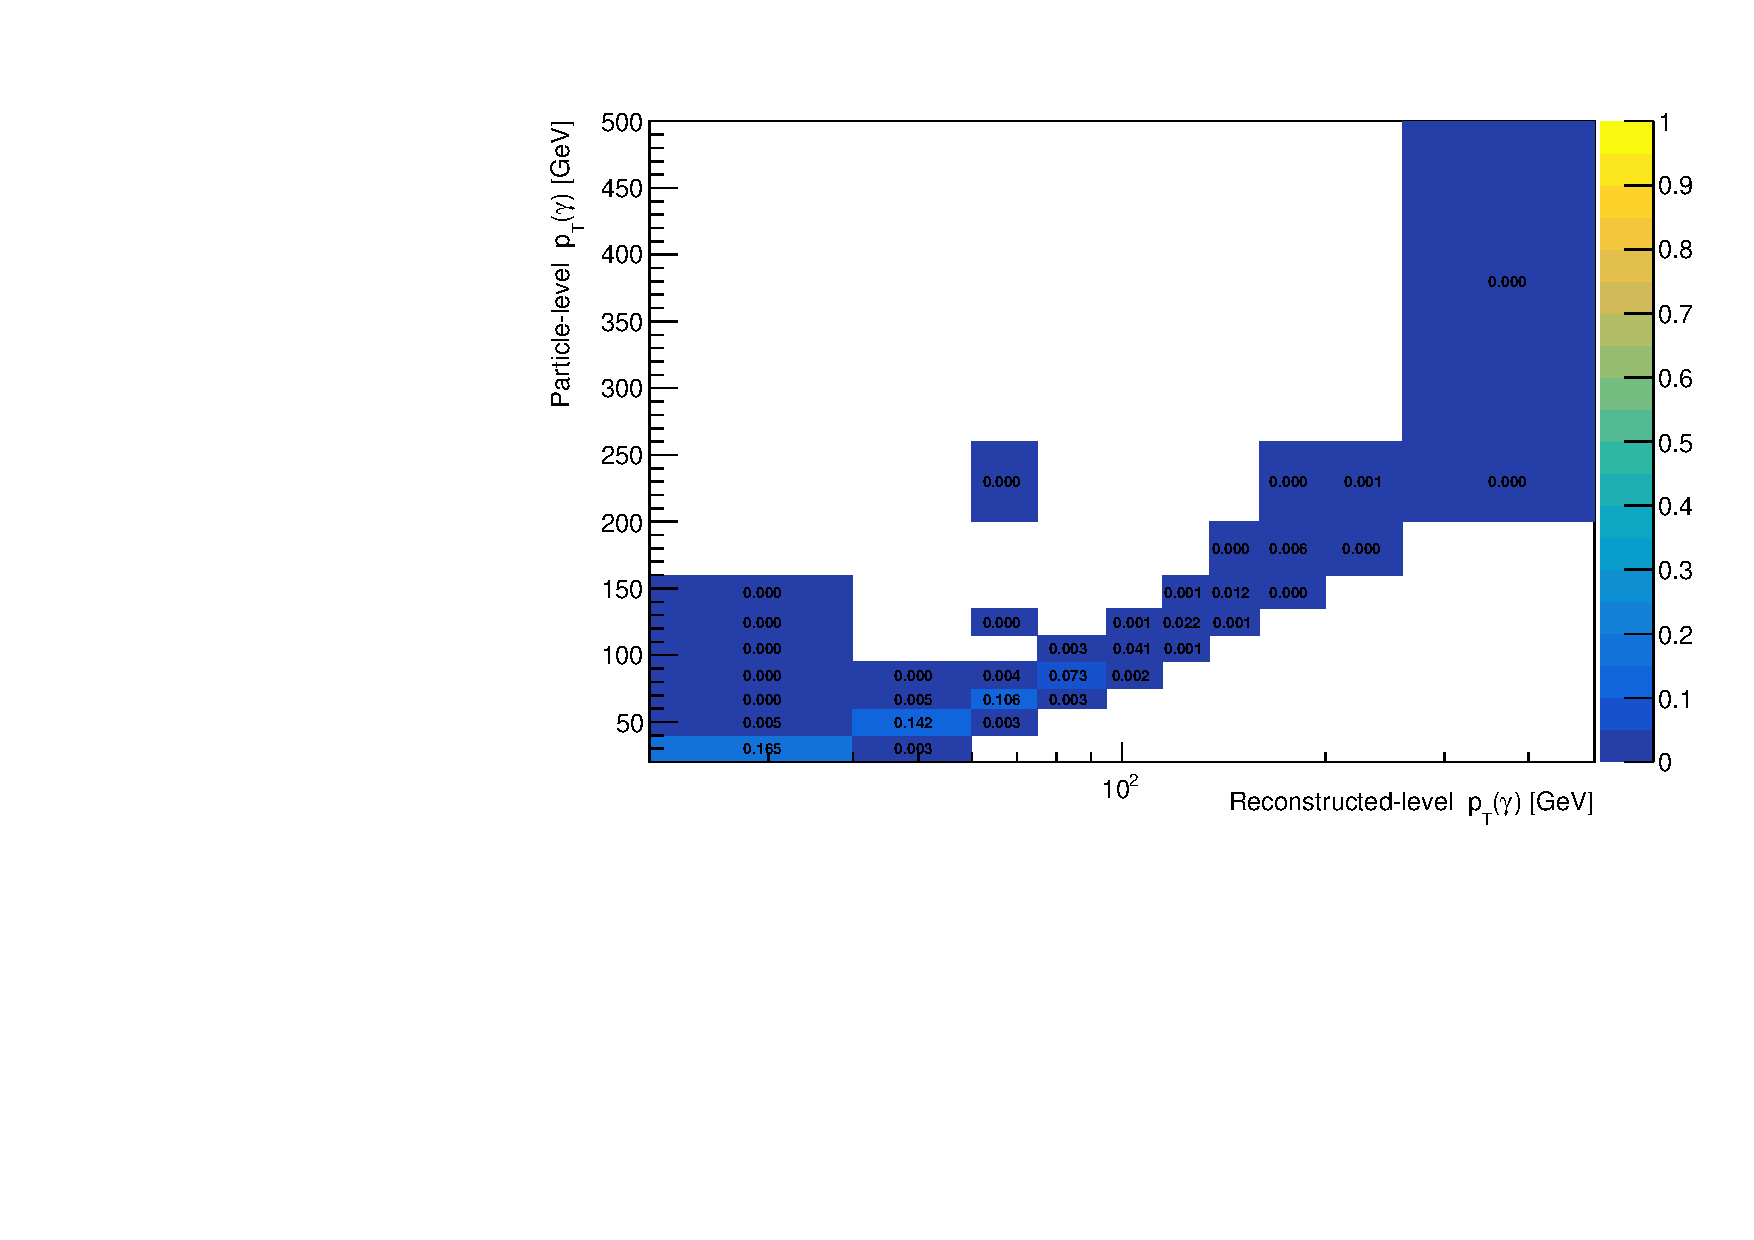
\includegraphics[width=0.3\textwidth]{figures/diff_xsec/ljet/Migration/response_h2_response_matrix_ph_pt_SR2.pdf}}
  \quad\quad
  \subfloat[]{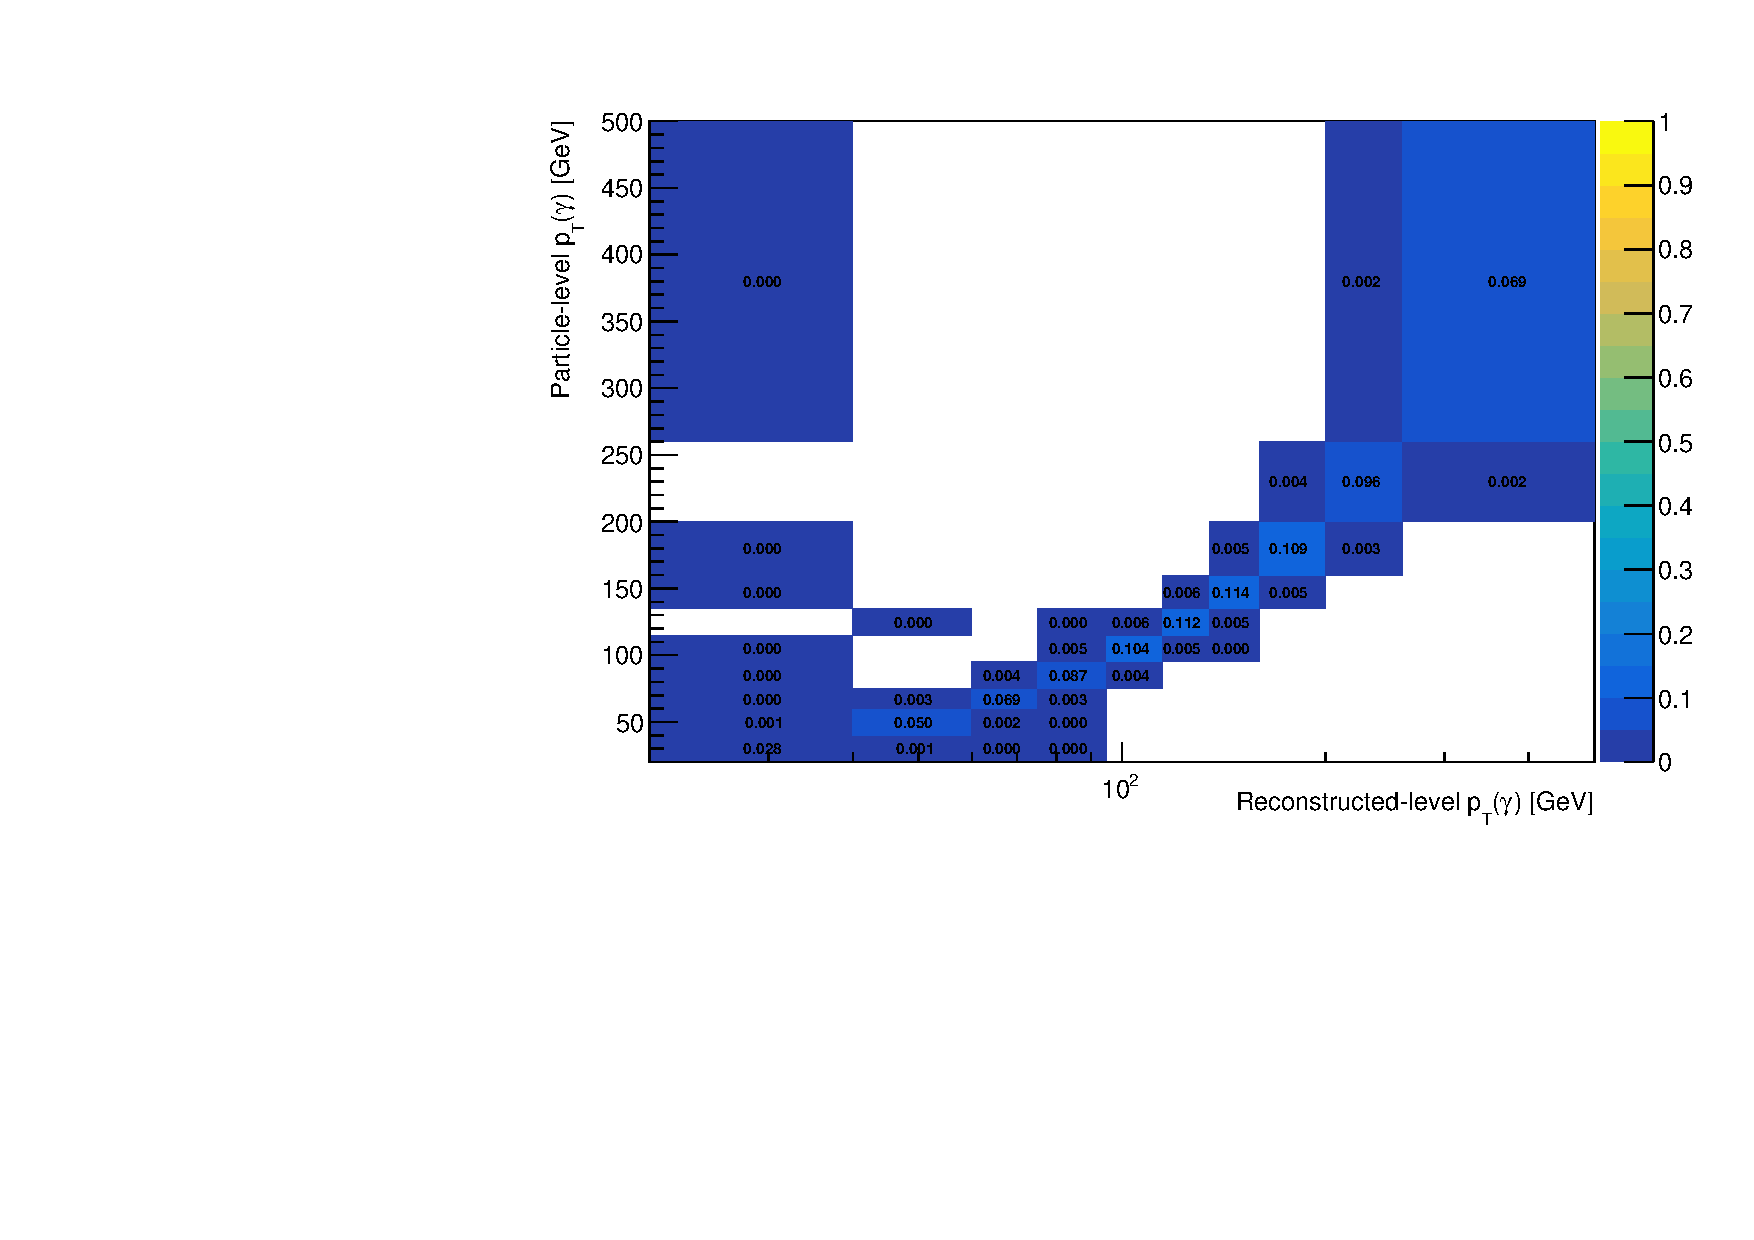
\includegraphics[width=0.3\textwidth]{figures/diff_xsec/ljet/Migration/response_h2_response_matrix_ph_pt_SR3.pdf}}
  \quad\quad
  \subfloat[]{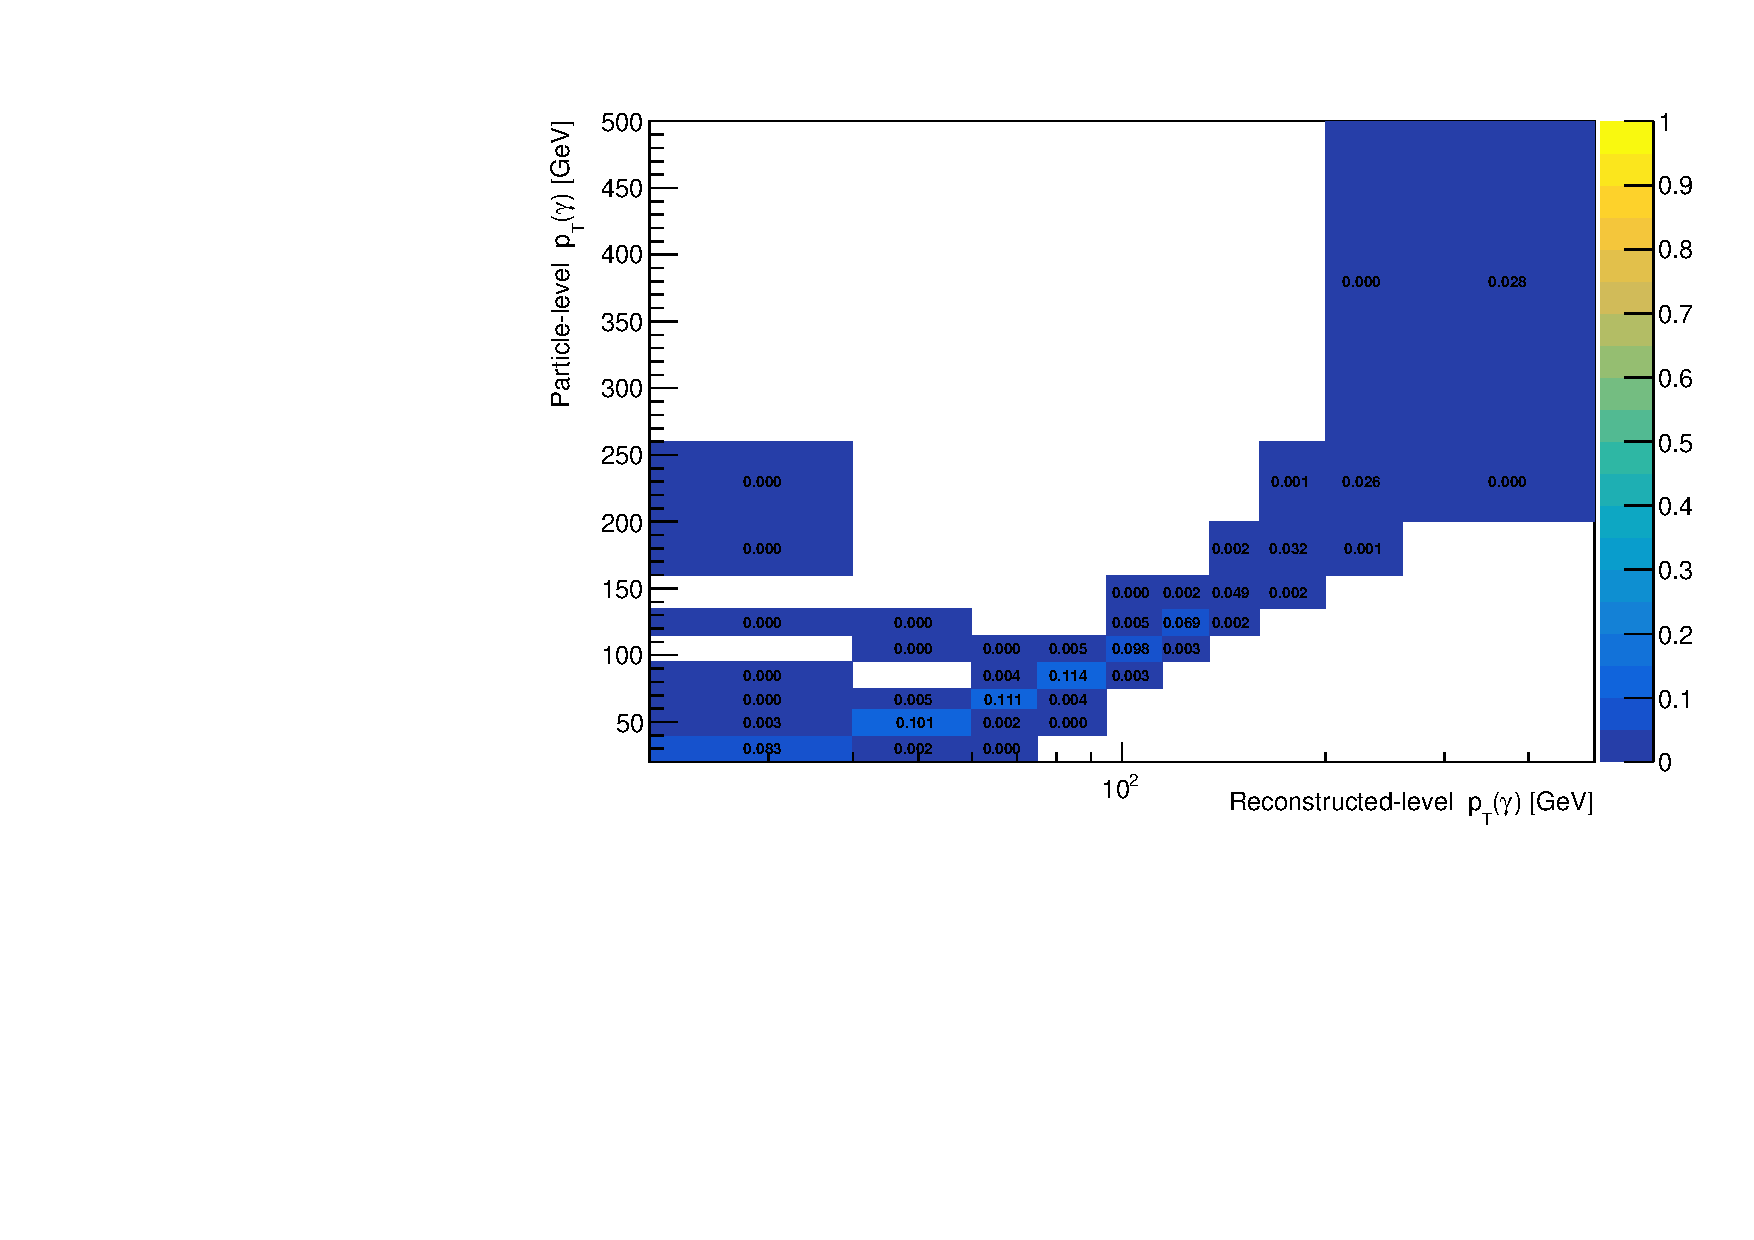
\includegraphics[width=0.3\textwidth]{figures/diff_xsec/ljet/Migration/response_h2_response_matrix_ph_pt_SR4.pdf}}
  \caption[Short caption for LoF]{Response matrices for the observable $p_T(\gamma)$ in the single-lepton channel, split across four regions determined. (a-d) Response matrices for the \tty production, \tty decay, fakes, and prompt photon enriched regions, respectively. -- \emph{Continued on next page}}
  \label{fig:folding_input_response_ljet_pt1}
\end{figure}
\begin{figure}[!ht]
  \ContinuedFloat
  \centering
  \subfloat[]{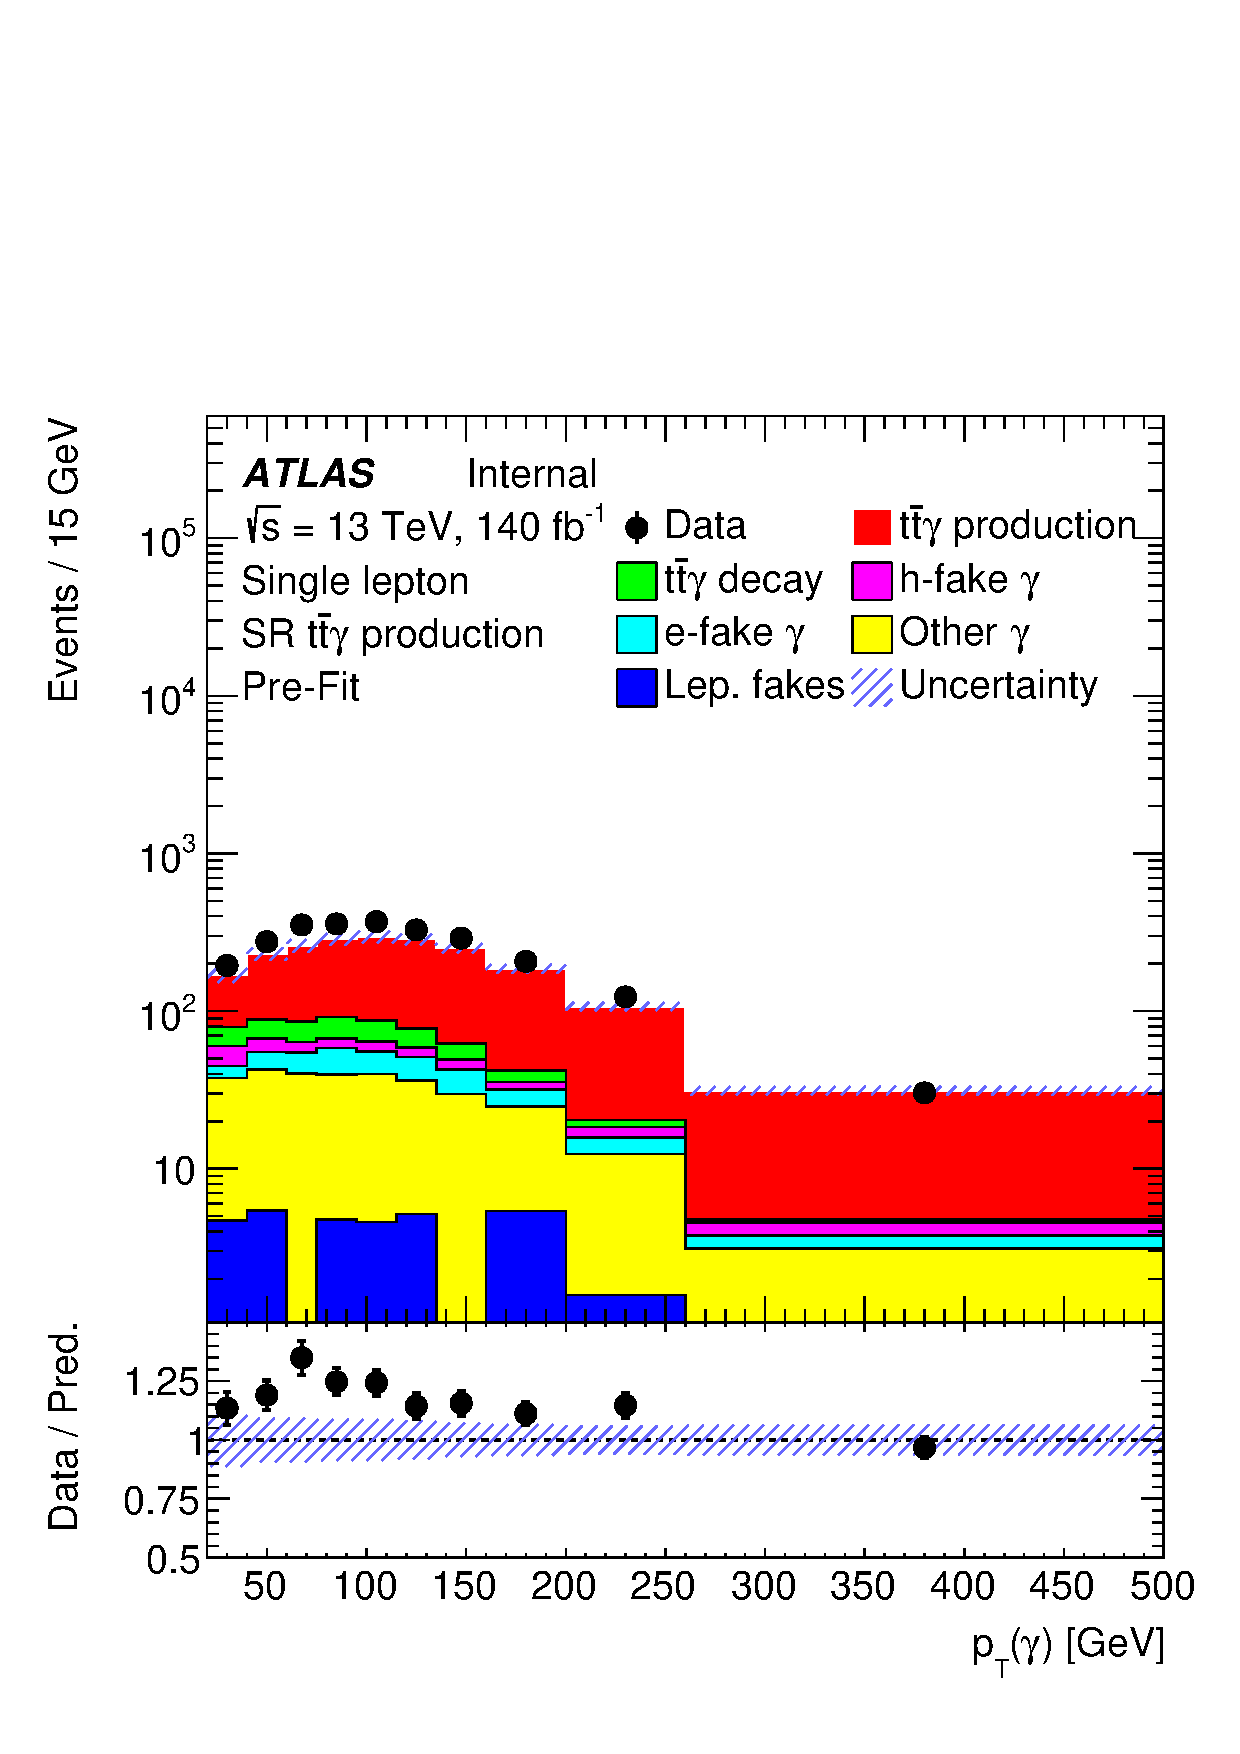
\includegraphics[width=0.3\textwidth]{figures/diff_xsec/ljet/Folded_distributions/tty1l_pt_all_syst/Plots/SR1.pdf}}
  \quad\quad
  \subfloat[]{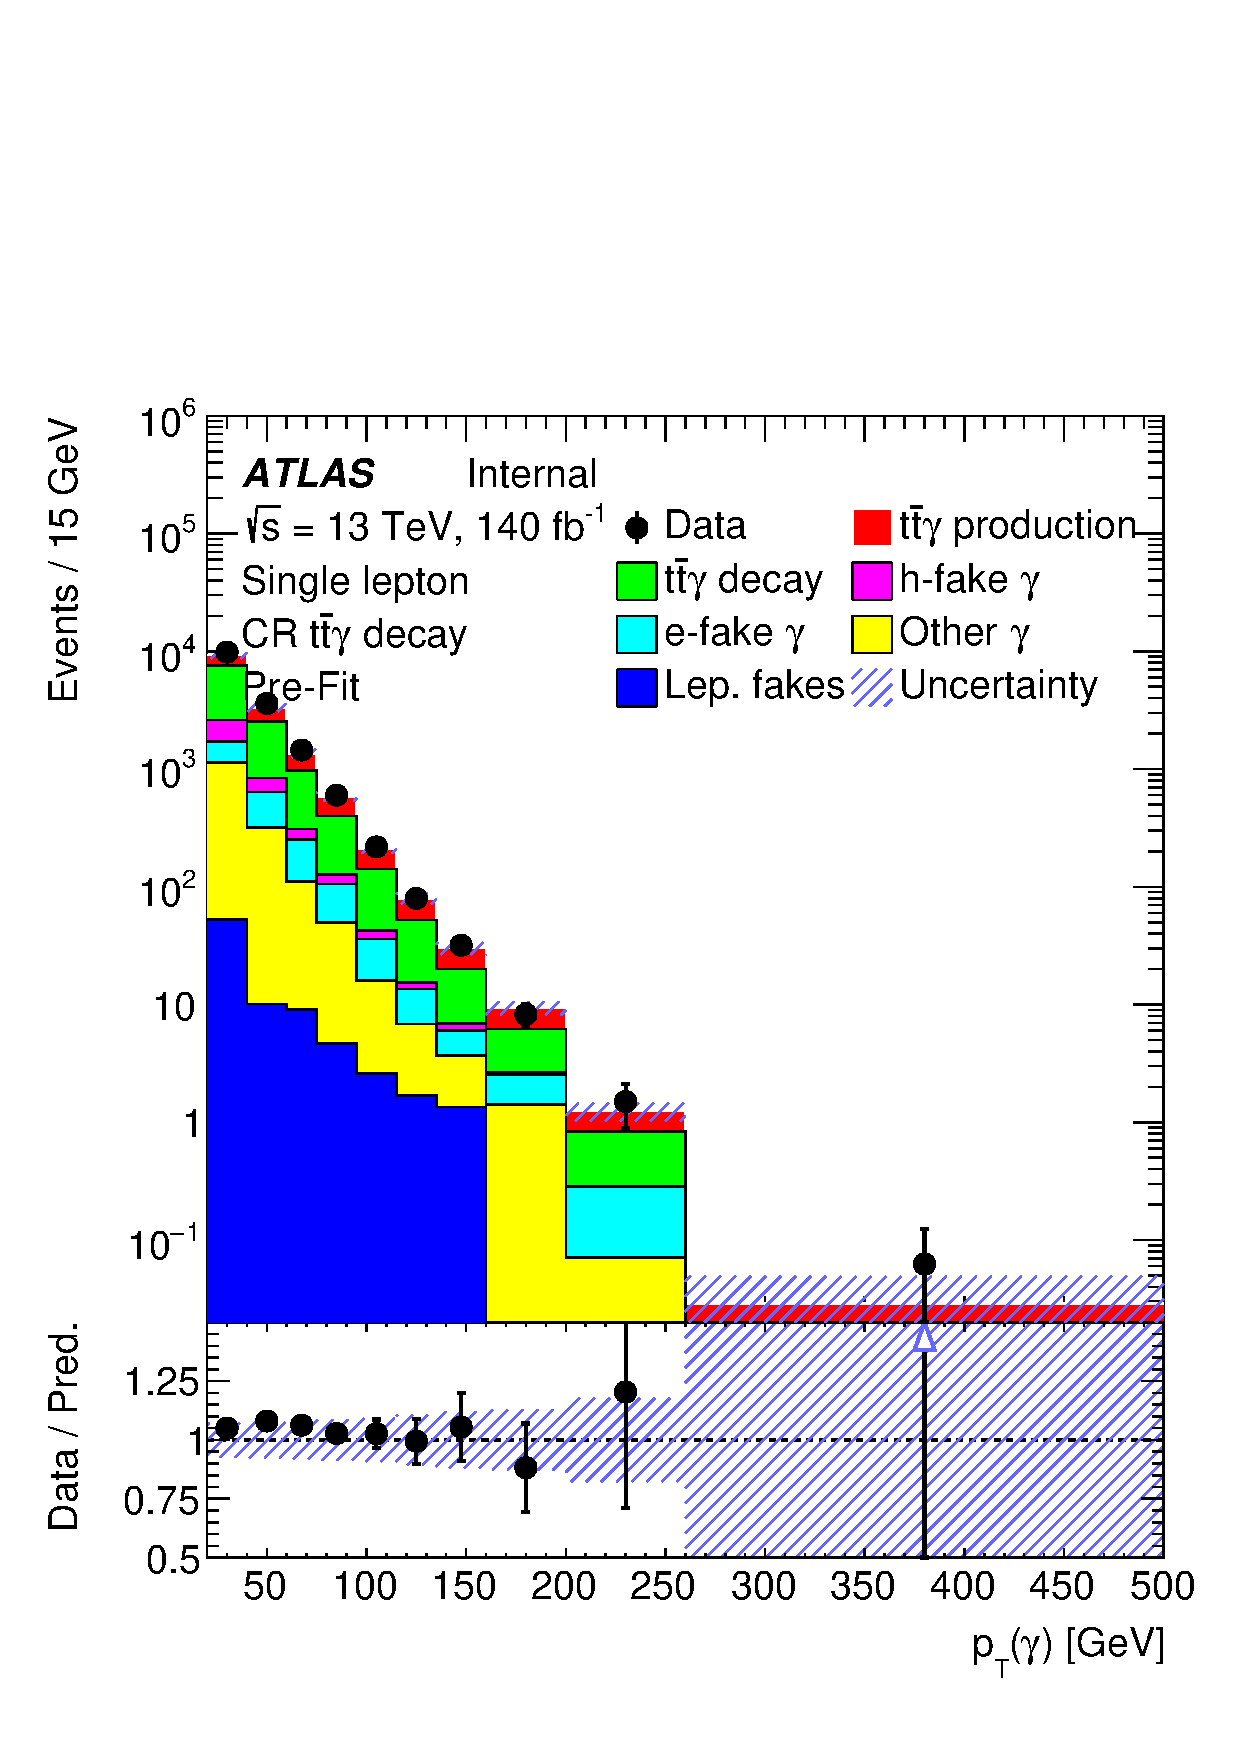
\includegraphics[width=0.3\textwidth]{figures/diff_xsec/ljet/Folded_distributions/tty1l_pt_all_syst/Plots/SR2.pdf}}
  \quad\quad
  \subfloat[]{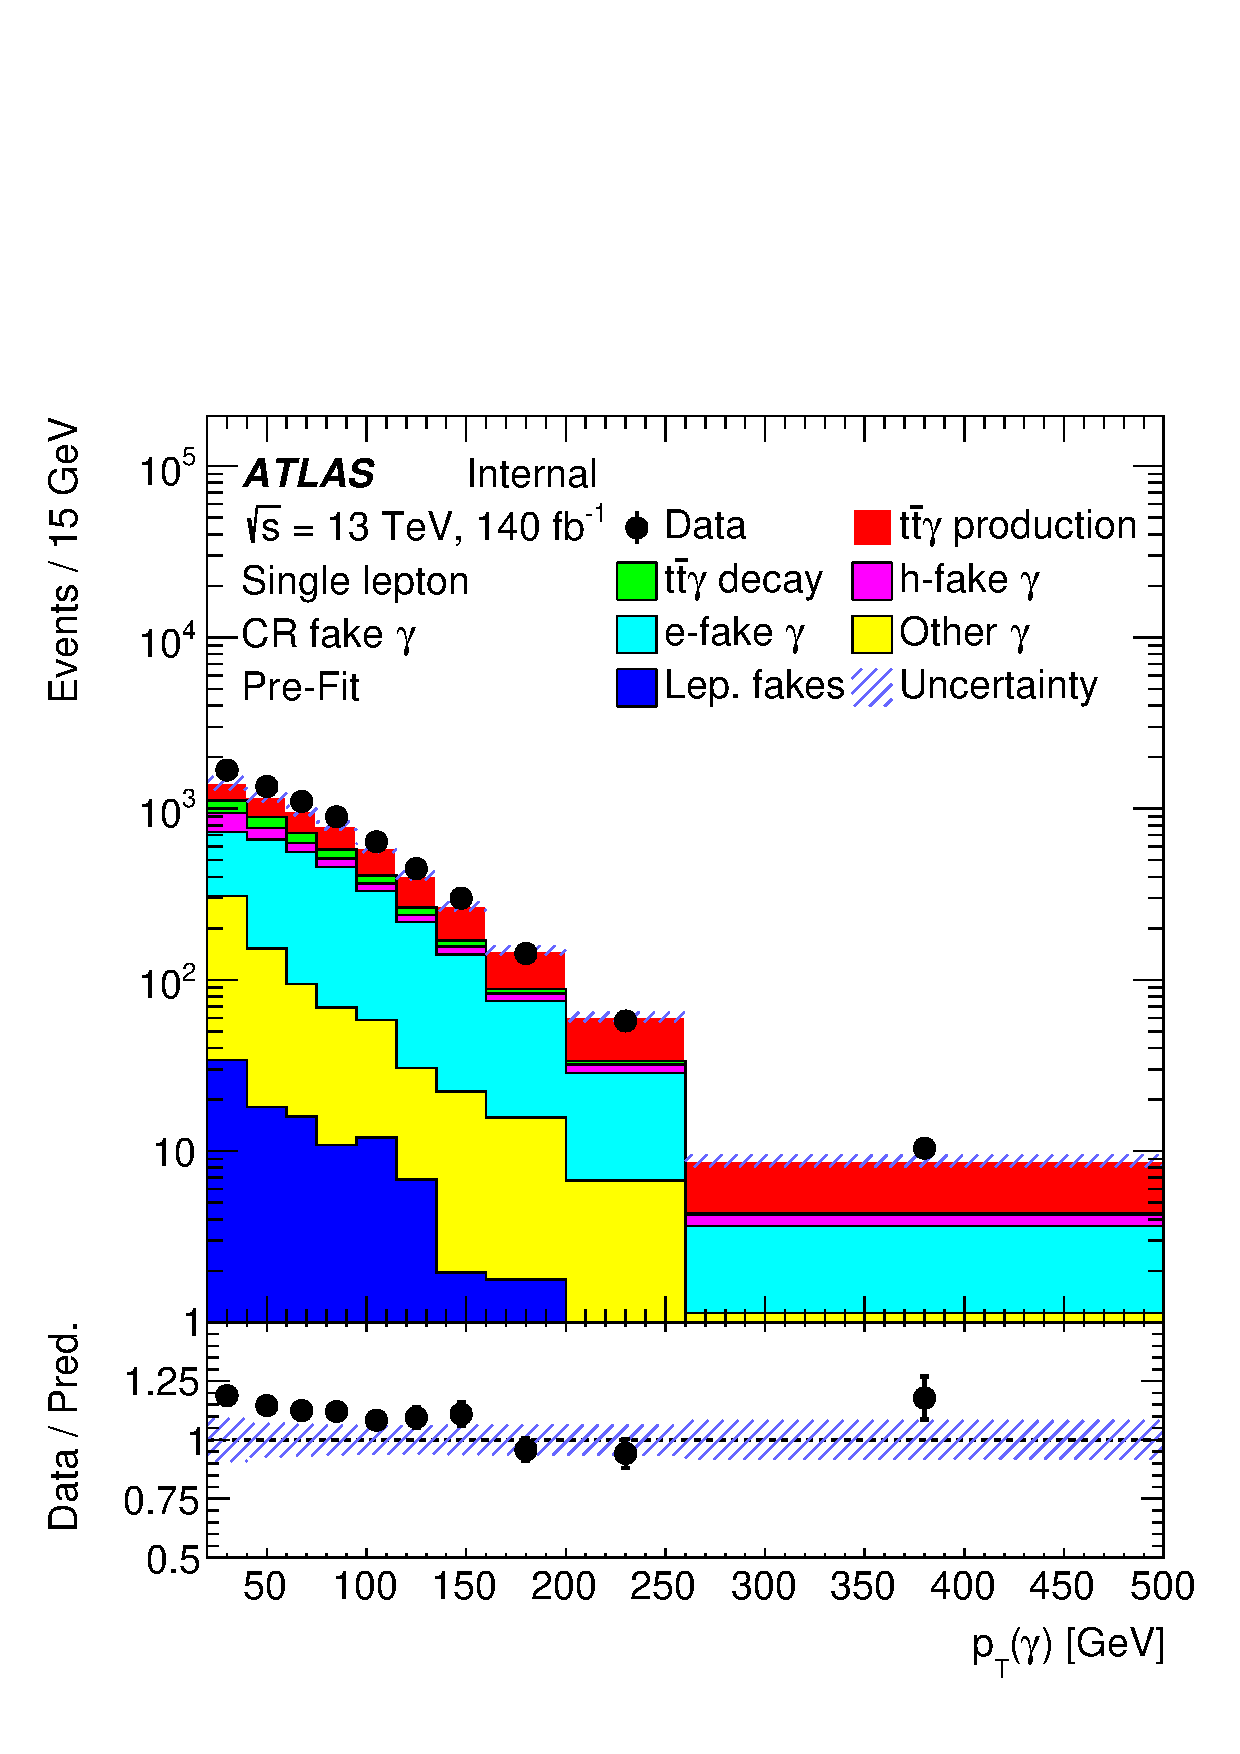
\includegraphics[width=0.3\textwidth]{figures/diff_xsec/ljet/Folded_distributions/tty1l_pt_all_syst/Plots/SR3.pdf}}
  \quad\quad
  \subfloat[]{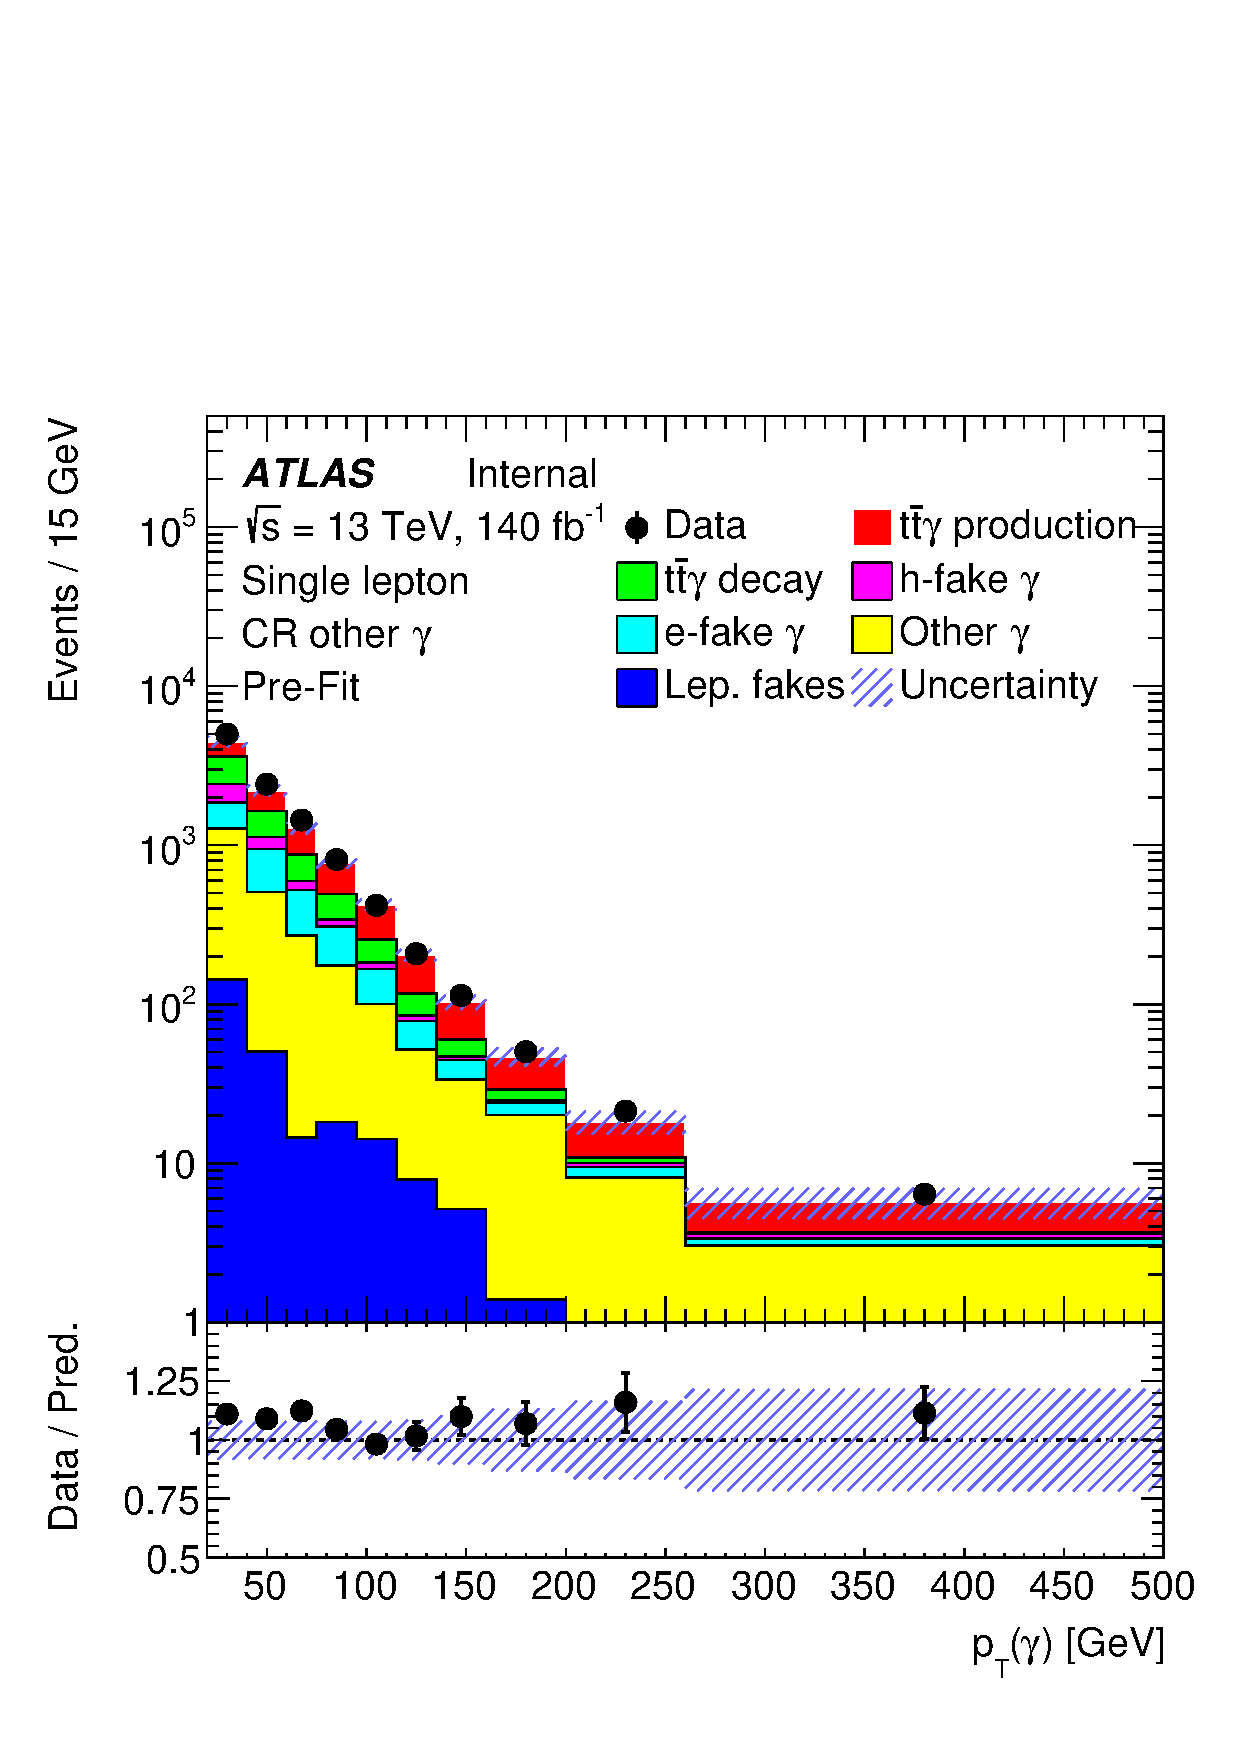
\includegraphics[width=0.3\textwidth]{figures/diff_xsec/ljet/Folded_distributions/tty1l_pt_all_syst/Plots/SR4.pdf}}
  \caption[]{(e-h) Corresponding Data-MC comparisons. The signal distribution at the reconstruction level was created by folding the truth distribution with the respective response matrix.}
  \label{fig:folding_input_response_ljet_pt2}
\end{figure}

%%%%%%%%
%  Migration matrices dilep
%%%%%%%%
\begin{figure}[ht]
    \centering
    \subfloat[]{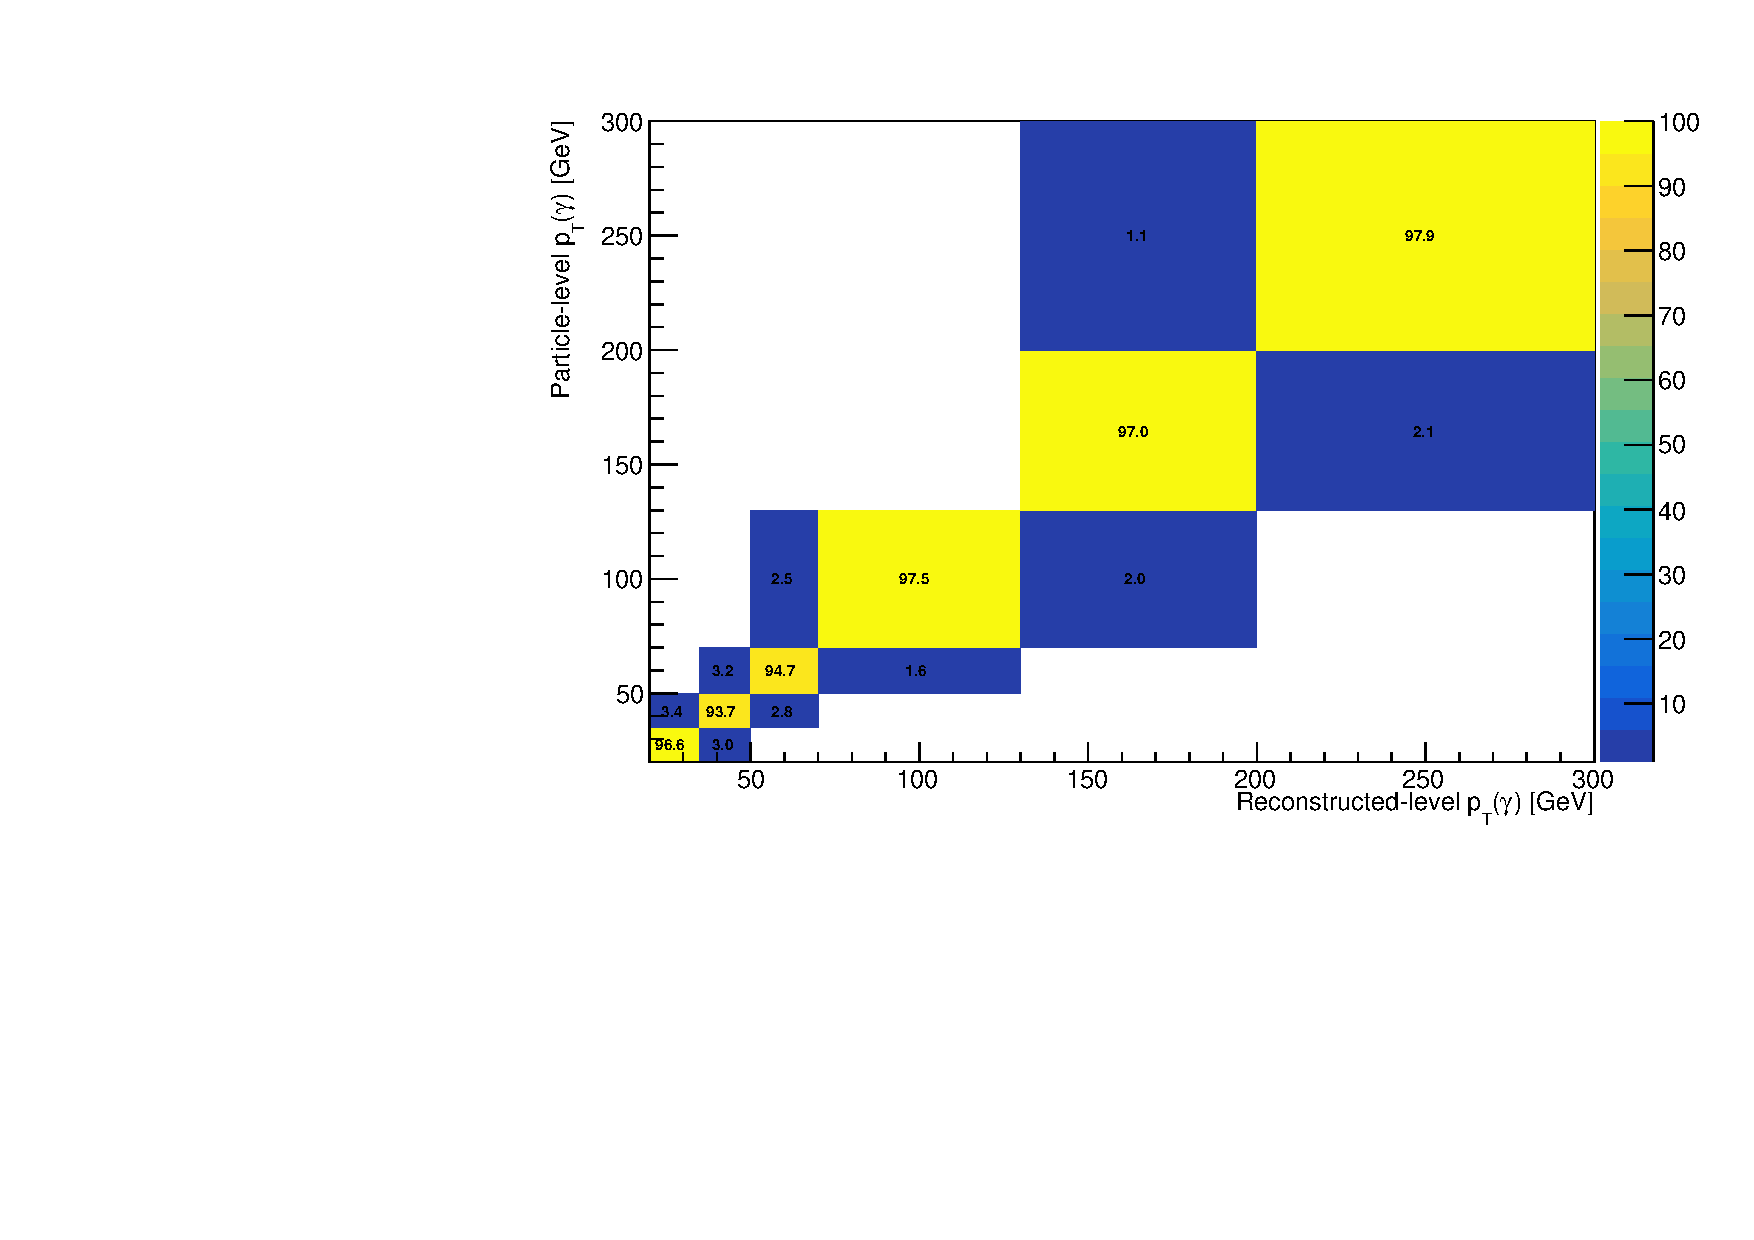
\includegraphics[width=0.3\textwidth]{figures/diff_xsec/dilep/Migration/migration_h2_ph_pt_reco_part_full_weighted_SR1.pdf}}
    \quad\quad
    \subfloat[]{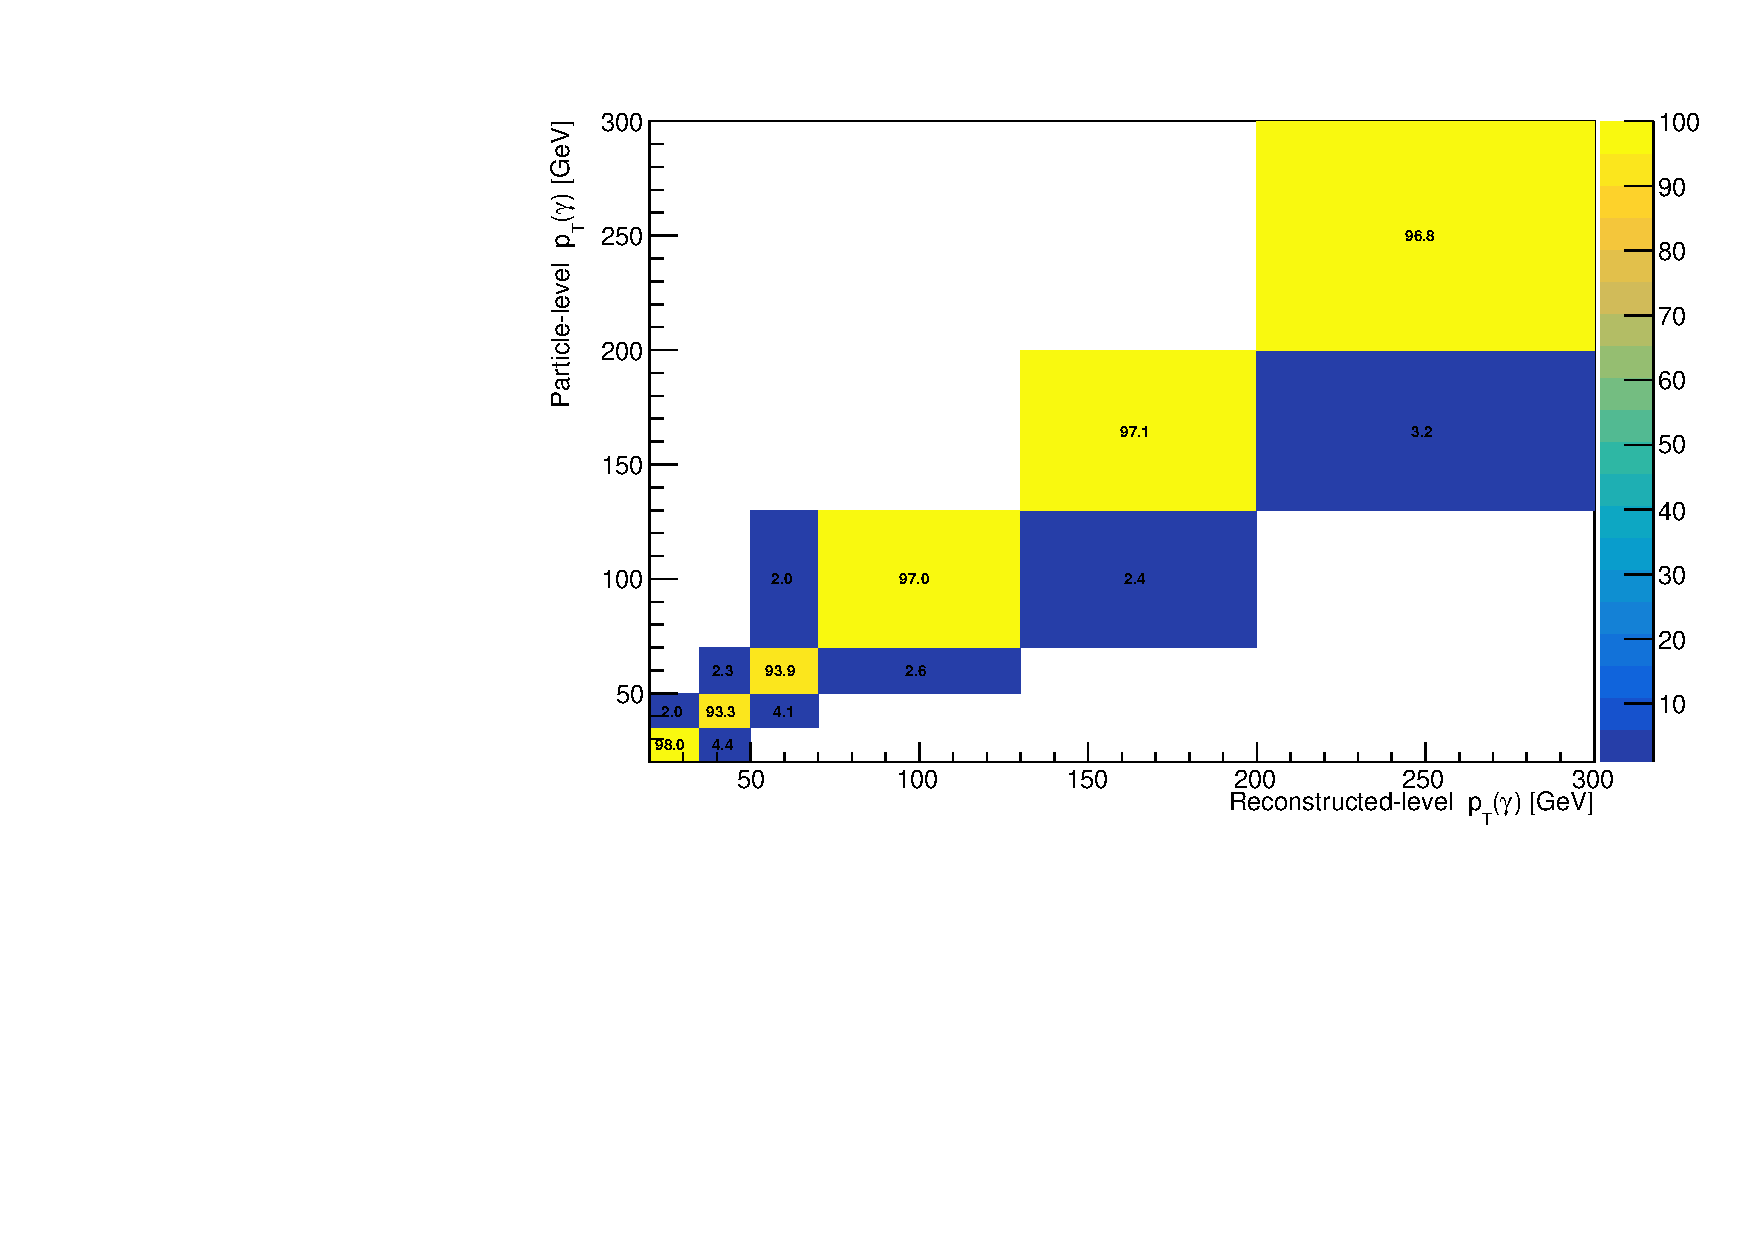
\includegraphics[width=0.3\textwidth]{figures/diff_xsec/dilep/Migration/migration_h2_ph_pt_reco_part_full_weighted_SR2.pdf}}

    \caption{The normalized migration matrices, $M_{\mathrm{r,t}}$ representing the migration of events from the particle level bin to the two regions at the reconstruction level: (a) $O_{\mathrm{NN}} \geq 0.6$ and (b) $O_{\mathrm{NN}} < 0.6$, for the observable $p_T(\gamma)$ in the dilepton channel.}
    \label{fig:folding_input_migration_dilep}
\end{figure}
\FloatBarrier

%%%%%%%%
%  Response matrices dilep
%%%
\begin{figure}[ht]
    \centering
    \subfloat[]{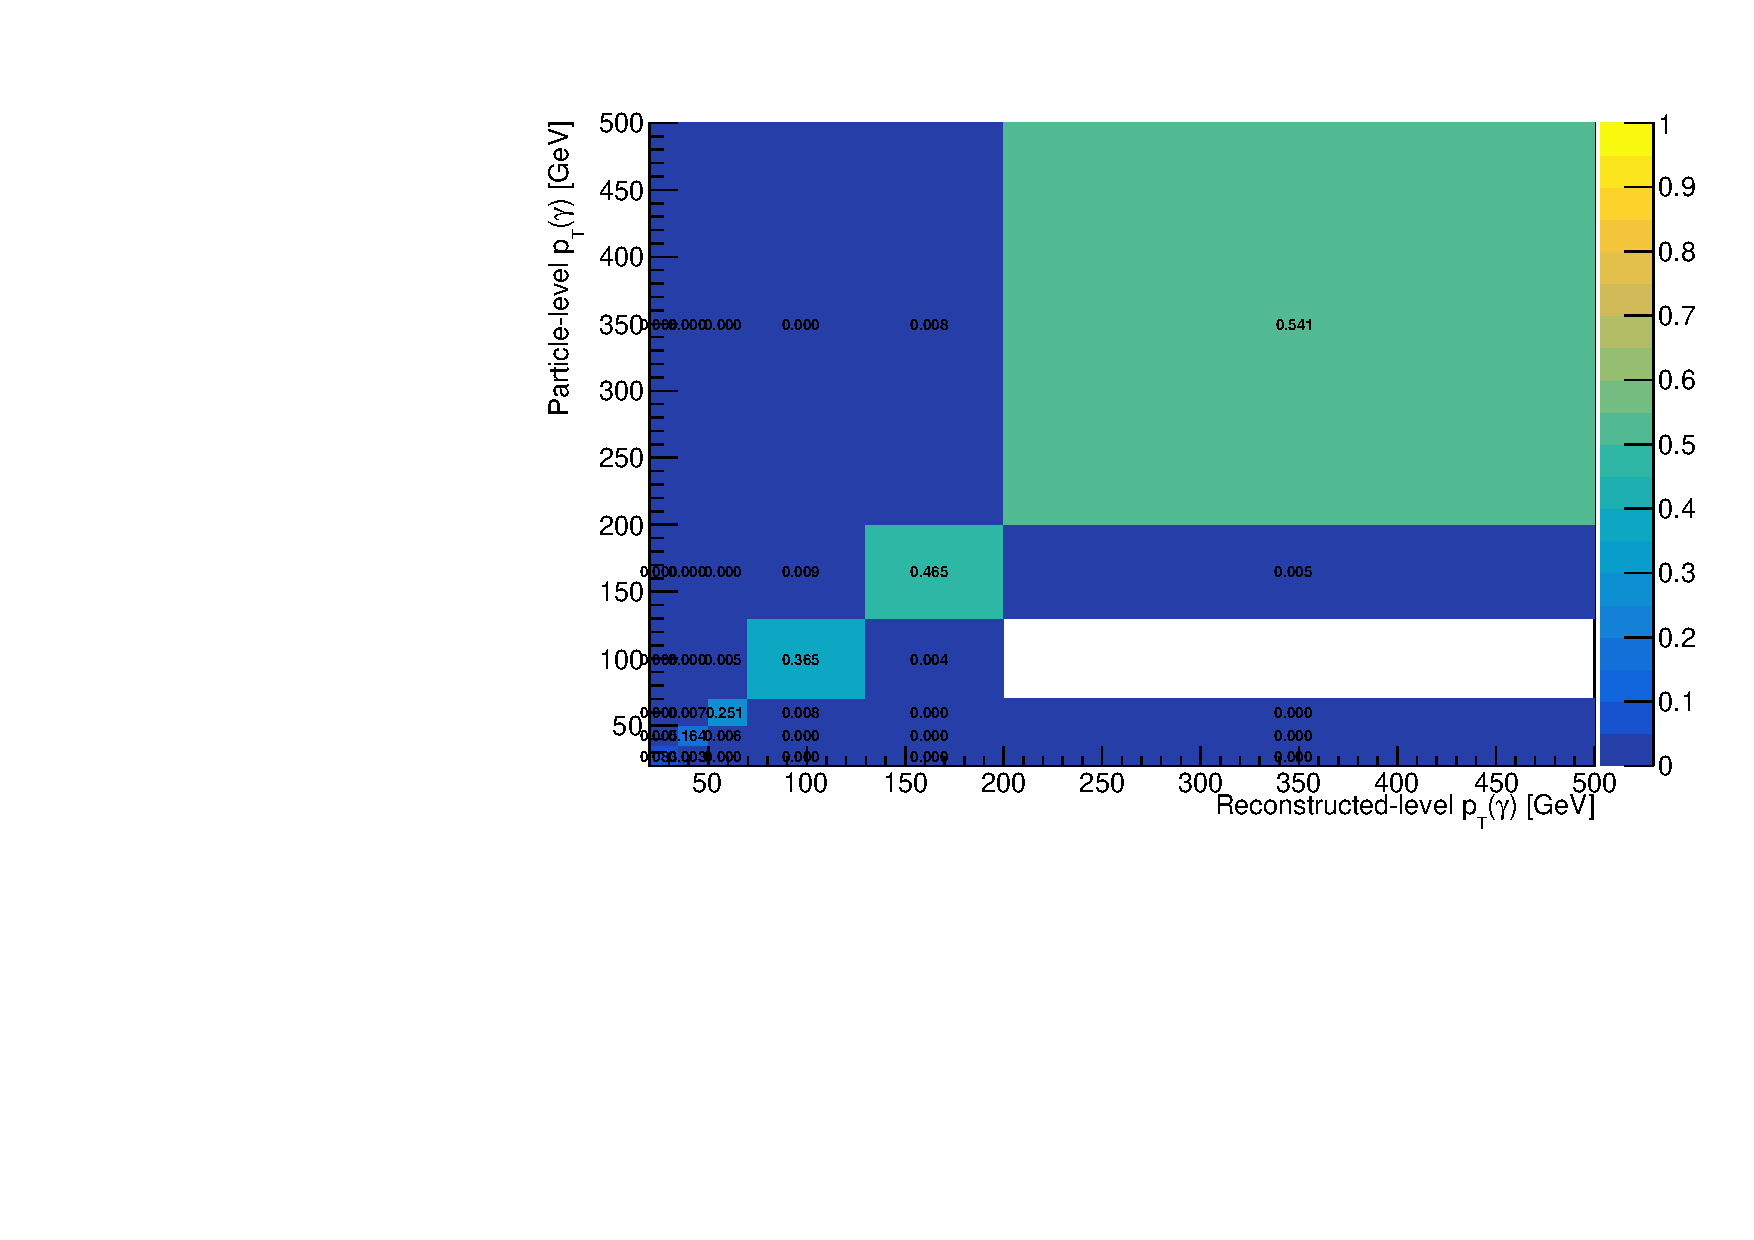
\includegraphics[width=0.3\textwidth]{figures/diff_xsec/dilep/Migration/response_h2_response_matrix_ph_pt_SR1.pdf}}
    \quad\quad
    \subfloat[]{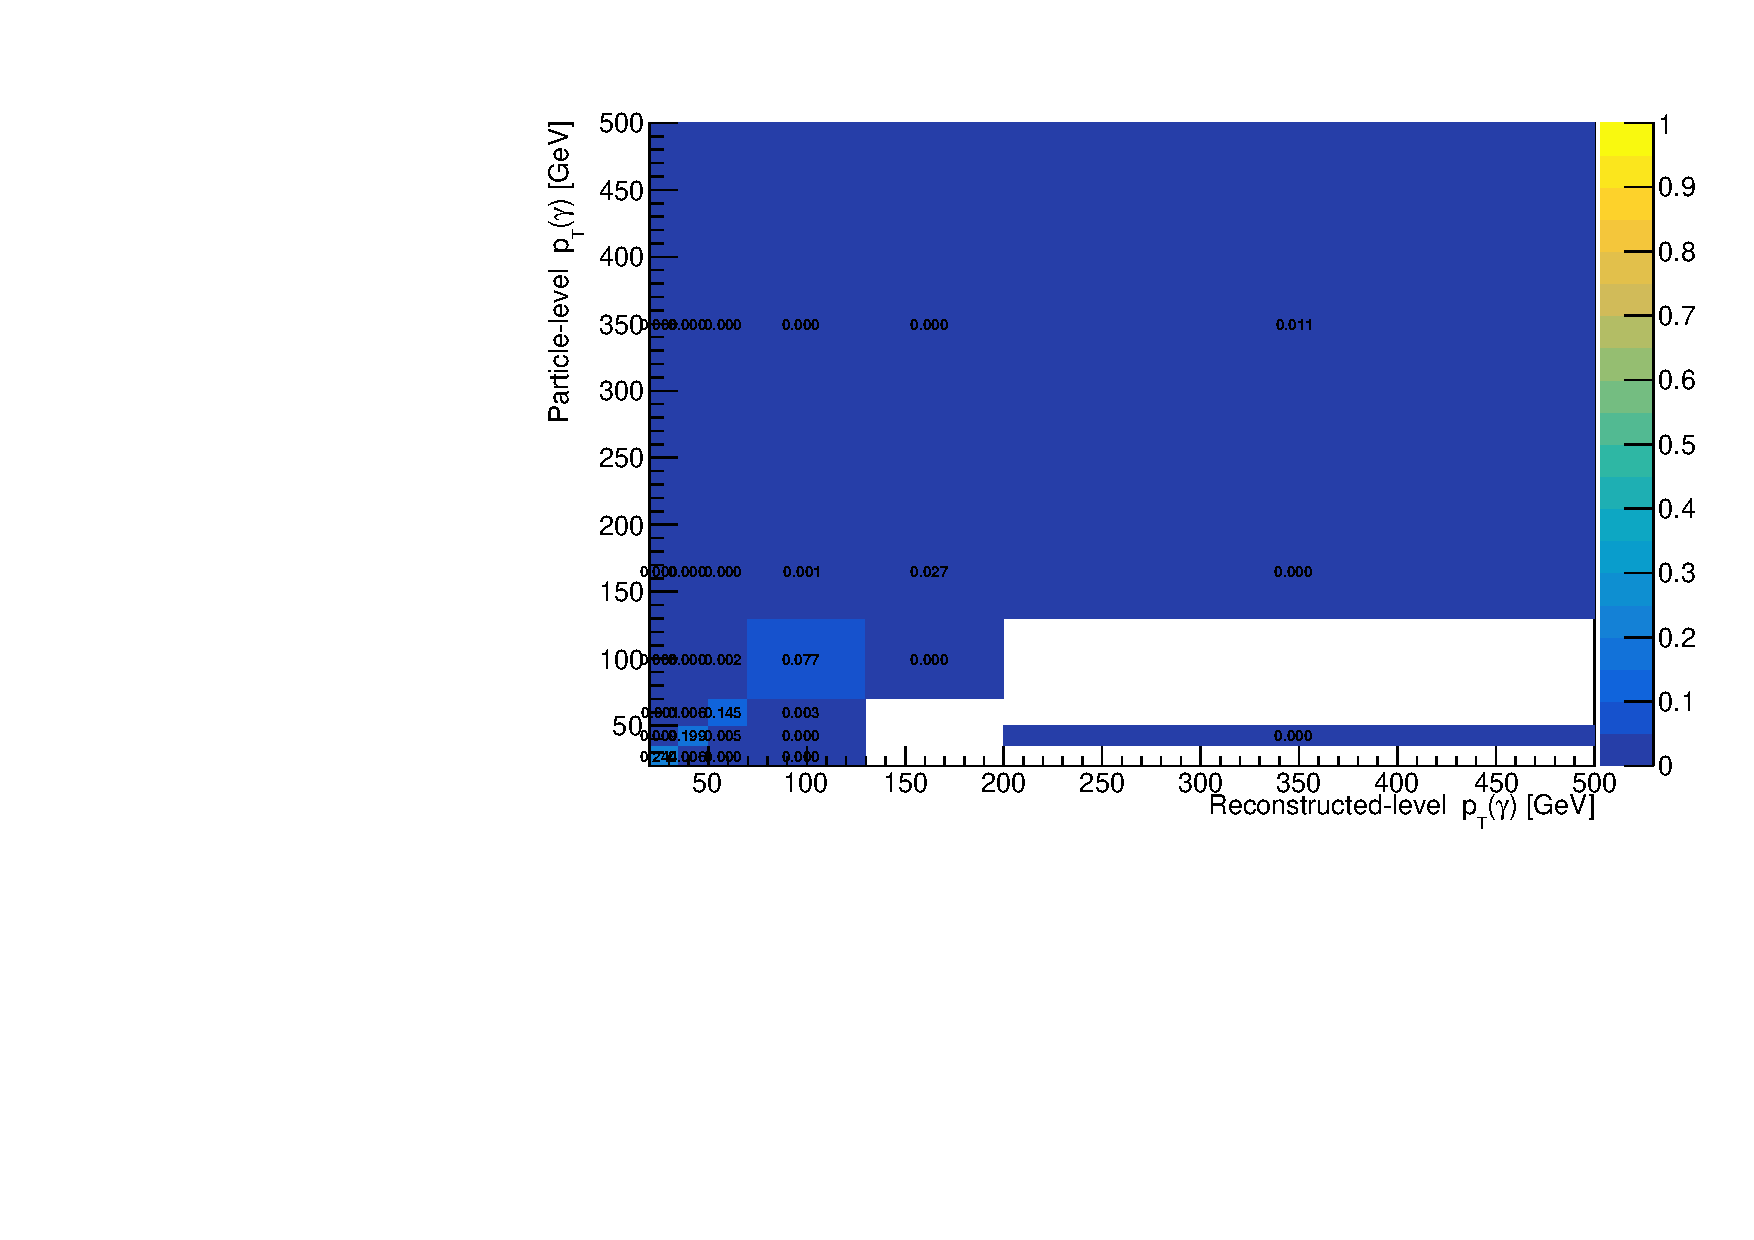
\includegraphics[width=0.3\textwidth]{figures/diff_xsec/dilep/Migration/response_h2_response_matrix_ph_pt_SR2.pdf}}
    \quad\quad
    \subfloat[]{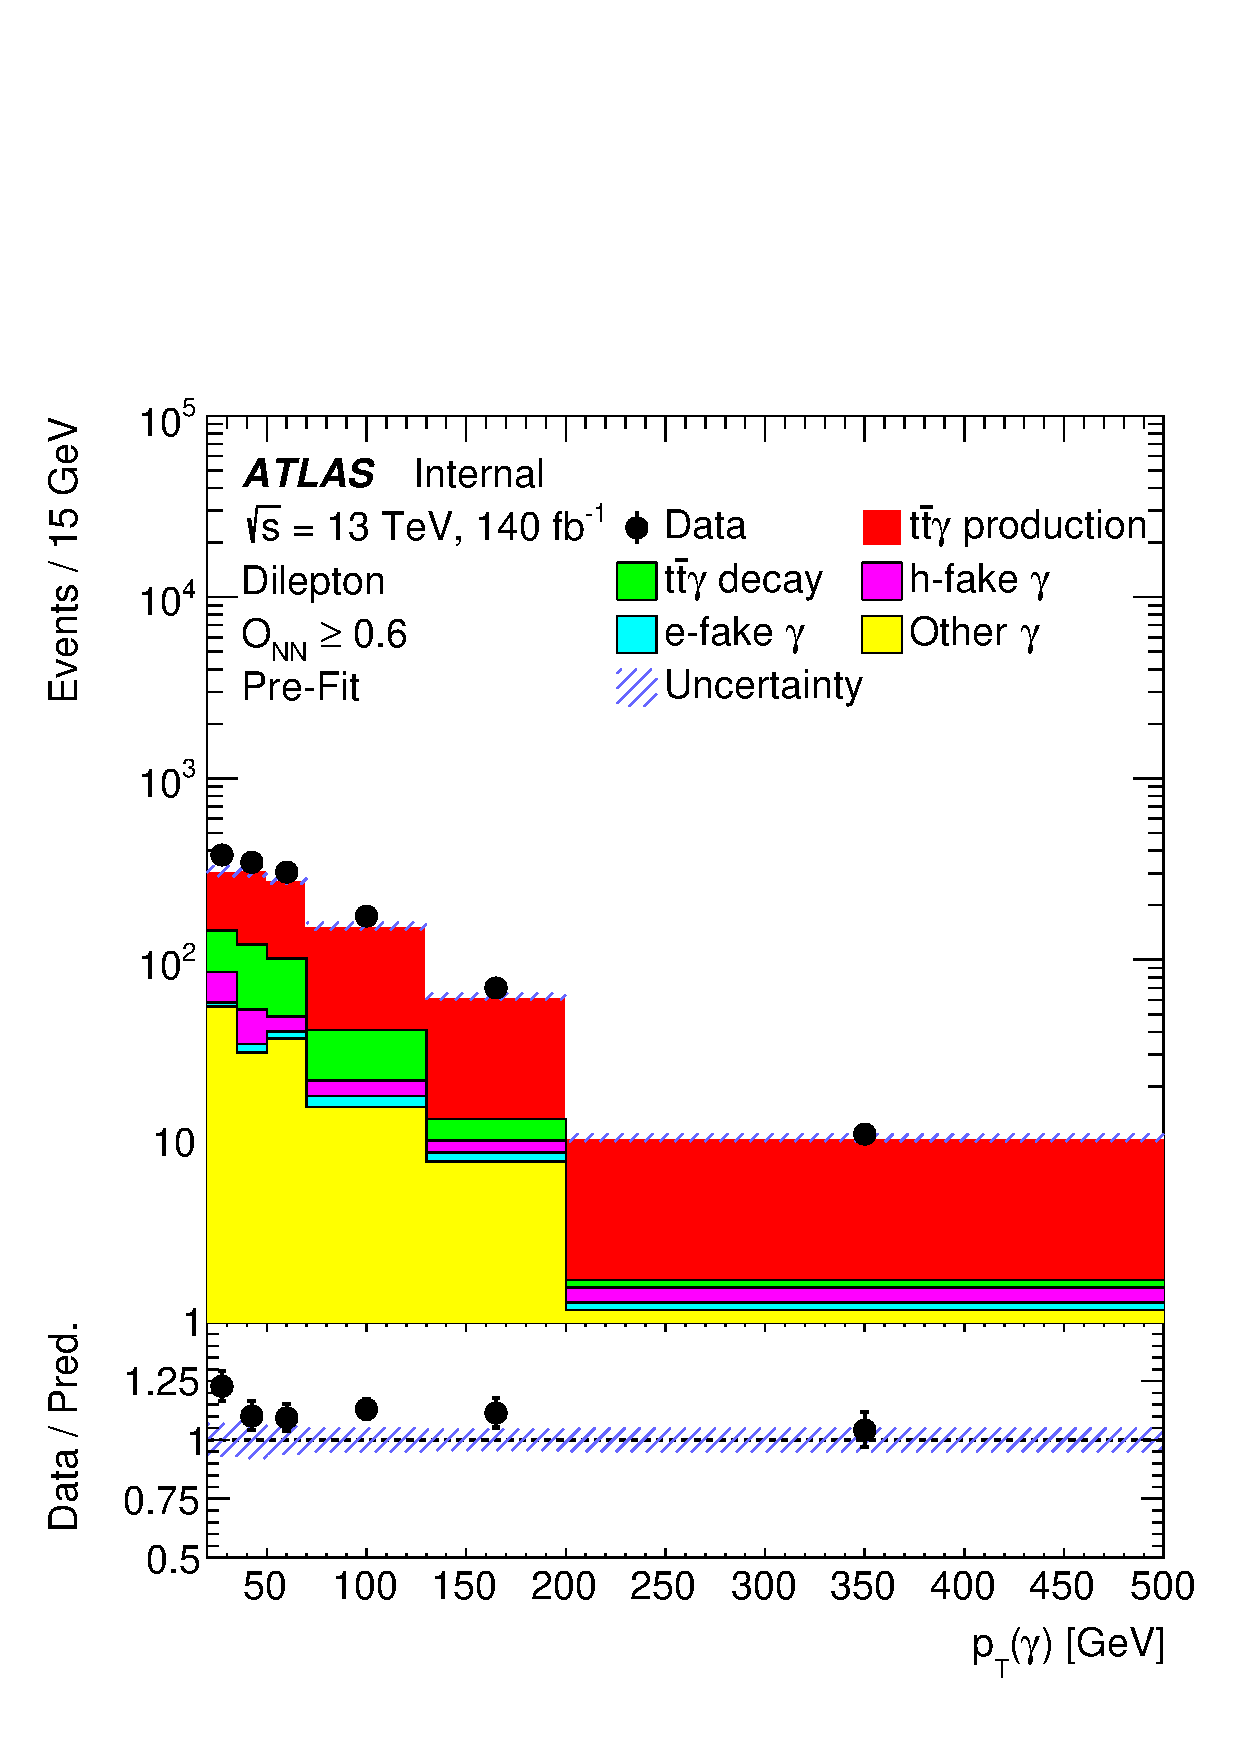
\includegraphics[width=0.3\textwidth]{figures/diff_xsec/dilep/Folded_distributions/tty2l_pt_all_syst/Plots/SR1.pdf}}
    \quad\quad
    \subfloat[]{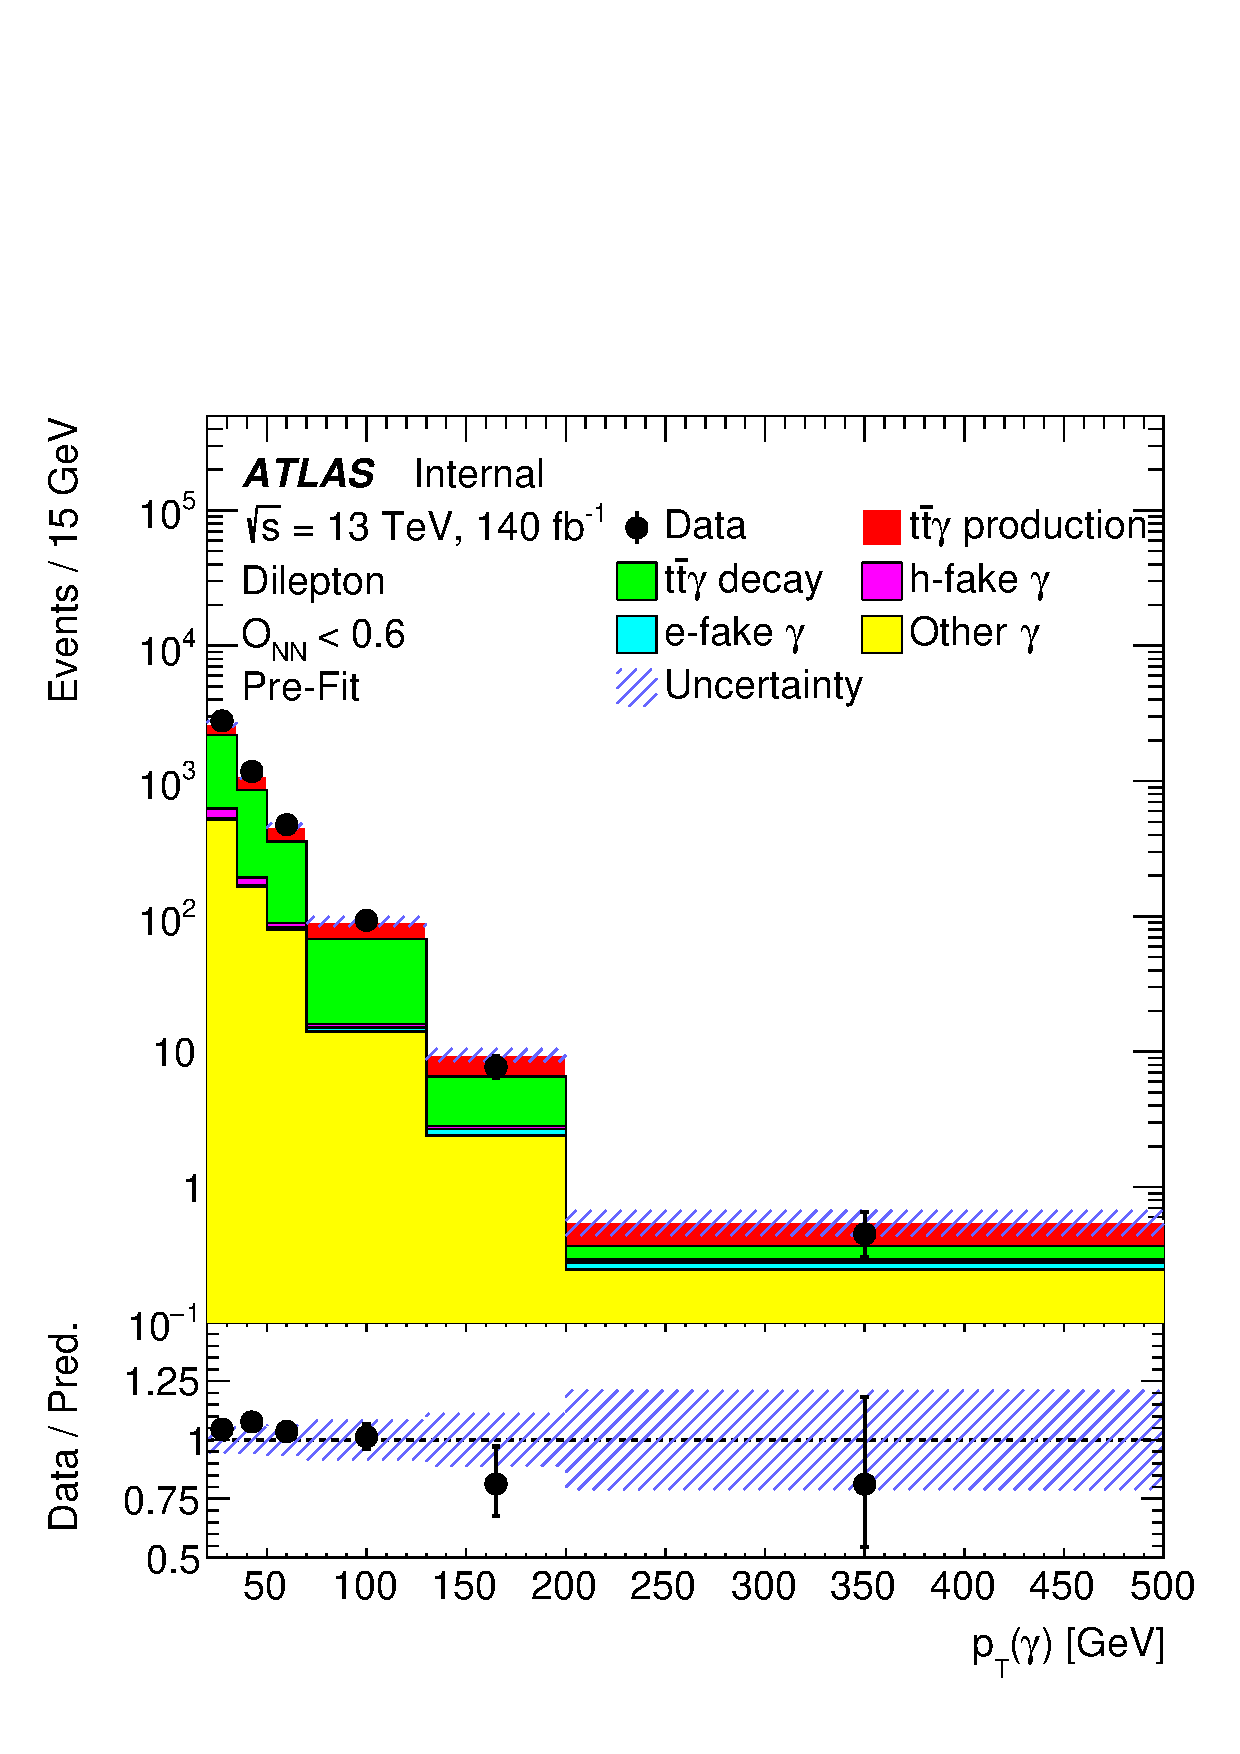
\includegraphics[width=0.3\textwidth]{figures/diff_xsec/dilep/Folded_distributions/tty2l_pt_all_syst/Plots/SR2.pdf}}
    \quad\quad
    \caption{Illustration of response matrices and data-MC comparison plots for the observable $p_T(\gamma)$ in dilepton channel. Subfigures: (a) Response matrix for $O_{\mathrm{NN}} \geq 0.6$. (b) Response matrix for $O_{\mathrm{NN}} < 0.6$. (c) Data-MC comparison for $O_{\mathrm{NN}} \geq 0.6$. (d) Data-MC comparison for $O_{\mathrm{NN}} < 0.6$. The signal distribution at the reconstruction level is created by folding the truth distribution with the corresponding response matrix.}
    \label{fig:folding_input_response_dilep}
\end{figure}
\FloatBarrier


\subsection{\tty production Measurement}
\label{sec:tty_prod_measurement}
%\textcolor{red}{To do: add results for inclusive \tty measurement (\tty production + decay), ongoing since the particle level information of \tty decay was missing until recently.}

This section presents the results of the unfolded likelihood fit to the real data for the \tty production cross section measurement. Profile likelihood unfolding method is performed to measure the cross-section from the data. The \tty decay template is kept free floating in this measurement.
After the fit, the fitted values of the POIs are shown in \cref{fig:pt_unfolded_ljet_table_realdata} and \cref{fig:pt_unfolded_dilep_table_realdata} for single-lepton channel and dilepton channel respectively. Using measured POIs, the post-fit distributions at the reconstruction level are shown in \cref{fig:pt_postfit_ljet_realdata} for the single-lepton channel and in \cref{fig:pt_postfit_dilep_realdata} for the dilepton channel. The distributions are only shown for the observable \ptgamma, rest are shown in the Appendix [ToDo].

As mentioned earlier the systematic uncertainties are taken into account as the nuisance parameter (NP) in the likelihood function and they are kept constrained. The best way to show the post-fit uncertainties is to quote using \textit{pulls} and \textit{constraints} of the NPs. The pull of a NP is defined as the difference between pre-fit and post-fit values of the parameter, normalized to the pre-fit uncertainty, $pull: = \frac{\hat{\theta}- \theta}{\delta \theta}$. The constraint is defined as the ratio between the post-fit and the pre-fit uncertainty of the NP. Through pulls and constraints, any possible issue in the fit can be identified. If NP is pulled too much that may be a hint that our estimate of the pre-fit value was not reasonable, where a constrained NP indicates that the data contains enough information to improve the precision of the NP with respect to the pre-fit estimate.Each data point in a pull plot represents a particular NP. The pull plots are shown in \cref{fig:pull_plot_pt_tty_dec_free_ljet_mu_blinded}, \cref{fig:pull_plot_pt_tty_dec_free_dilep_mu_blinded_1}, \cref{fig:pull_plot_pt_tty_dec_free_dilep_mu_blinded_2}. % explain the observation which NP are constrained and pulled and which are not

The correlation is calculated among the POIs and the NPs shown in \cref{fig:NP_corr_ljet_mu_blinded} and in \cref{fig:NP_corr_dilep_mu_blinded}, for the single lepton and dilepton channels respectively (only shown for \ptgamma ). The post-fit value of all the NPs changed within 1 $\sigma$, with a large fraction of the NPs having very small pulls and constraints, which indicates that the fit is robust and not affected by any unexpected behavior of the NPs. % explain the observation which NPs are correlated and which are not

The impact of the NPs on the measurement of the POIs is shown using the Ranking plot. The impact is calculated by varying each NP by $\pm 1 \sigma$ while keeping others at the post-fit value and measuring the change in the POIs. Ranking plots are shown in \cref{fig:ranking_ljet_prod} and \cref{fig:ranking_dilep_prod} for single lepton and dilepton channels (shown for \ptgamma).% explain the observation which NPs are highly ranked and which are not

The unfolded distributions at particle level are shown in \cref{fig:pt_unfolded_ljet_dist_realdata} and \cref{fig:pt_unfolded_dilep_dist_realdata_1}, \cref{fig:pt_unfolded_dilep_dist_realdata_2} for single lepton and dilepton channels. The normalized unfolded distributions are shown in \cref{fig:tty_prod_diff_Ljets_norm} and \cref{fig:tty_prod_diff_DL1_norm}, \cref{fig:tty_prod_diff_DL2_norm} for single lepton and dilepton channels respectively. The decomposed uncertainties of the unfolded distributions for the absolute differential cross-sections are illustrated in \cref{fig:tty_prod_diff_Ljets_groupedimpact} and \cref{fig:tty_prod_diff_DL1_groupedimpact}, \cref{fig:tty_prod_diff_DL2_groupedimpact} for single lepton channel and dilepton channel respectively. $\chi^2$/ndf and $p$-values between the measured absolute and normalised cross-sections of \tty production and the NLO \MGNLO simulations interfaced with \PYTHIA[8] and \HERWIG[7] are shown in Table ~\ref{tab:chi2_ttyprod}.


\begin{figure}[ht]
  \centering
  \subfloat[]{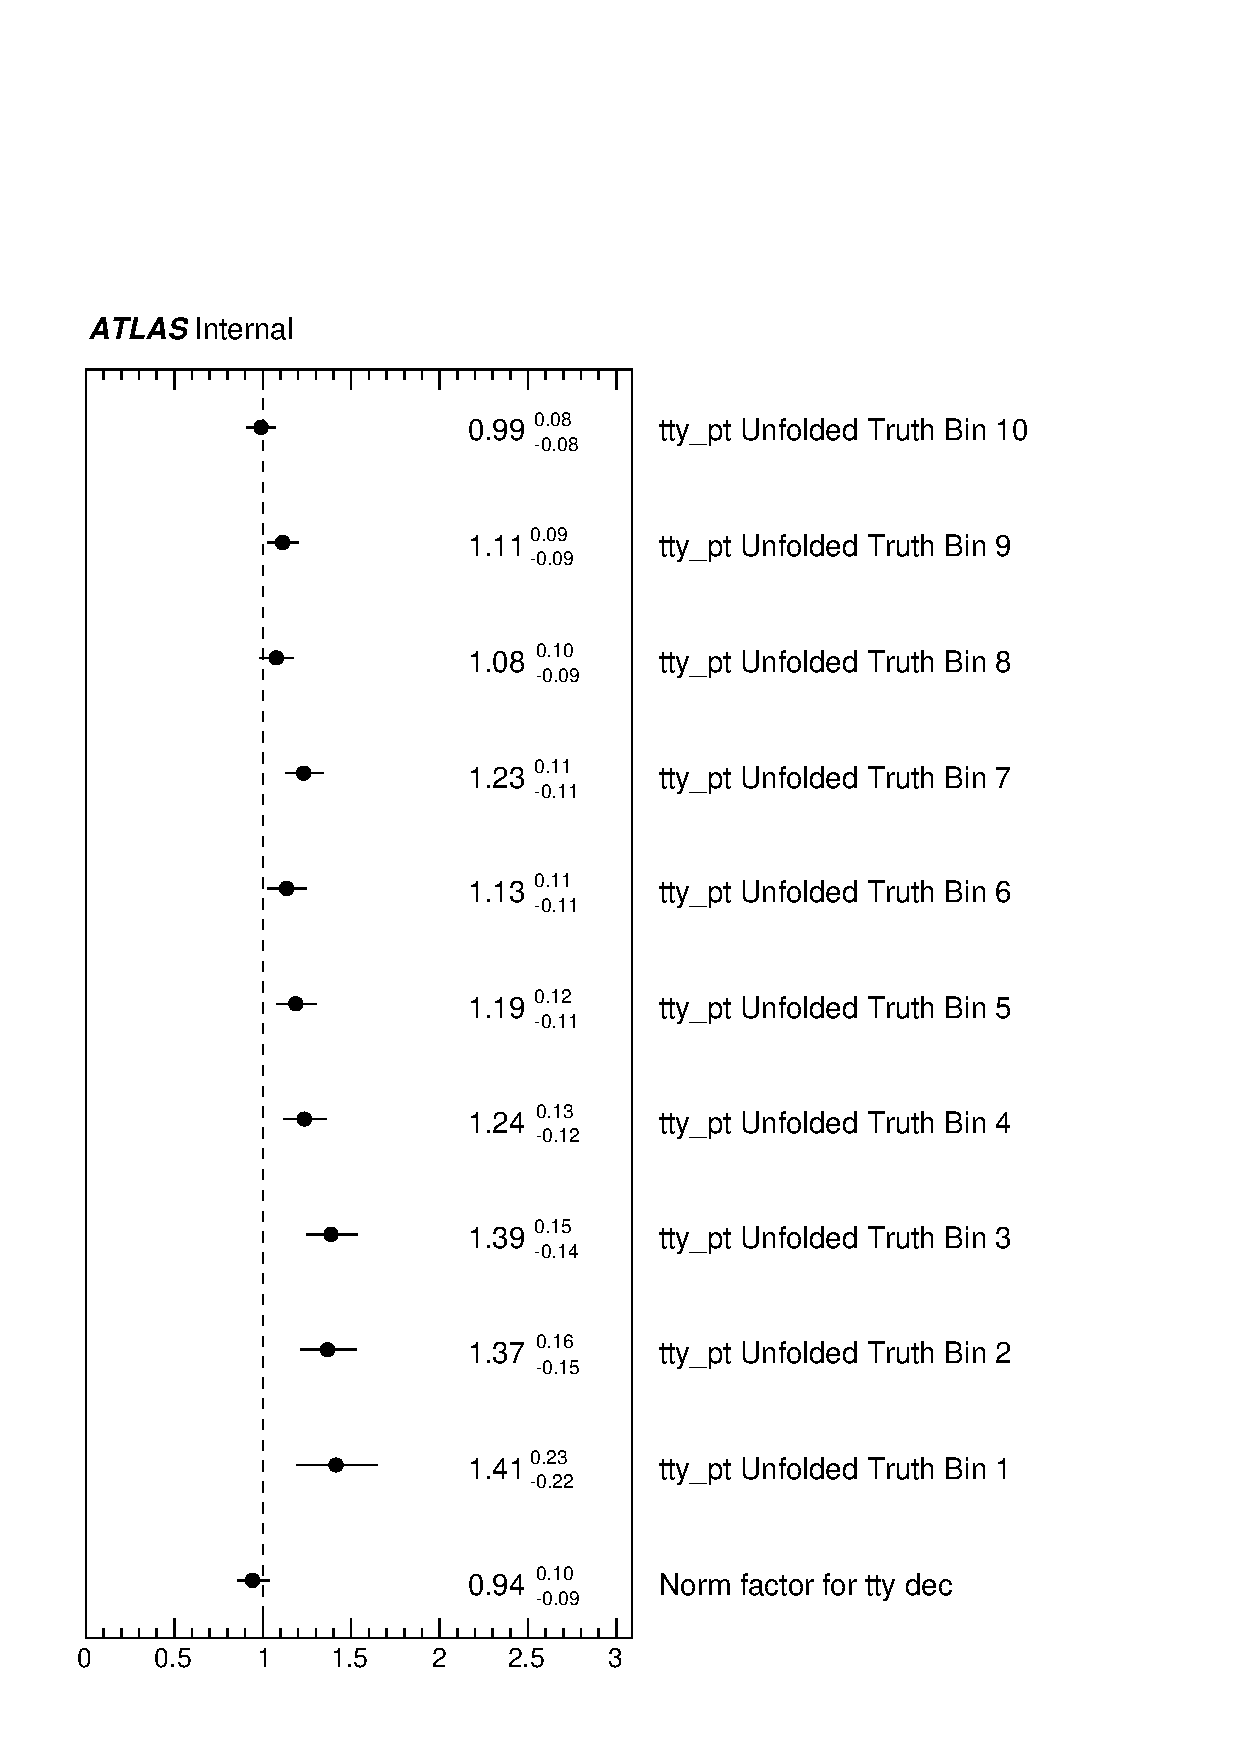
\includegraphics[width=0.3\textwidth]{figures/diff_xsec/ljet_tty_prod_mu_blinded/Unfolded_data/tty1l_pt_all_syst/NormFactors.pdf}}
  \quad
  \subfloat[]{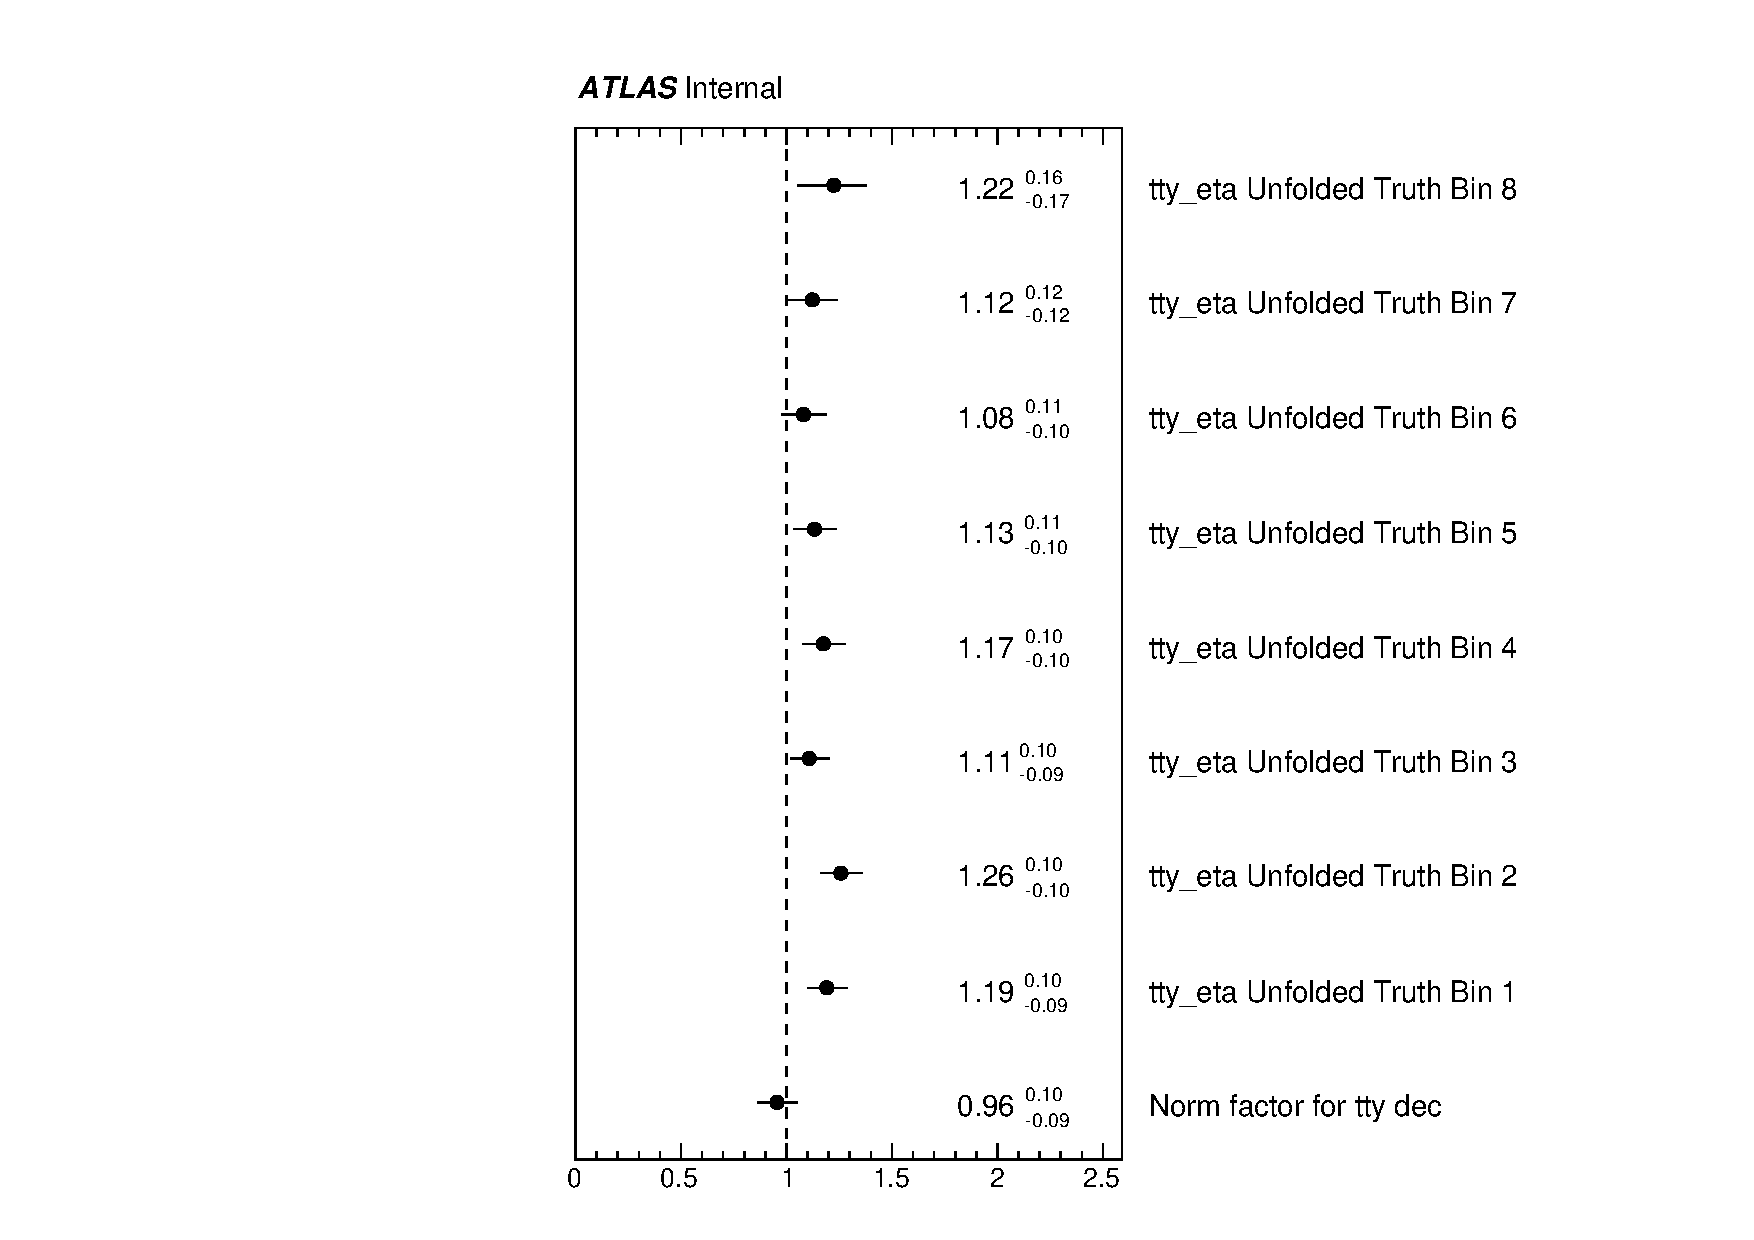
\includegraphics[width=0.3\textwidth]{figures/diff_xsec/ljet_tty_prod_mu_blinded/Unfolded_data/tty1l_eta_all_syst/NormFactors.pdf}}
  \quad
  \subfloat[]{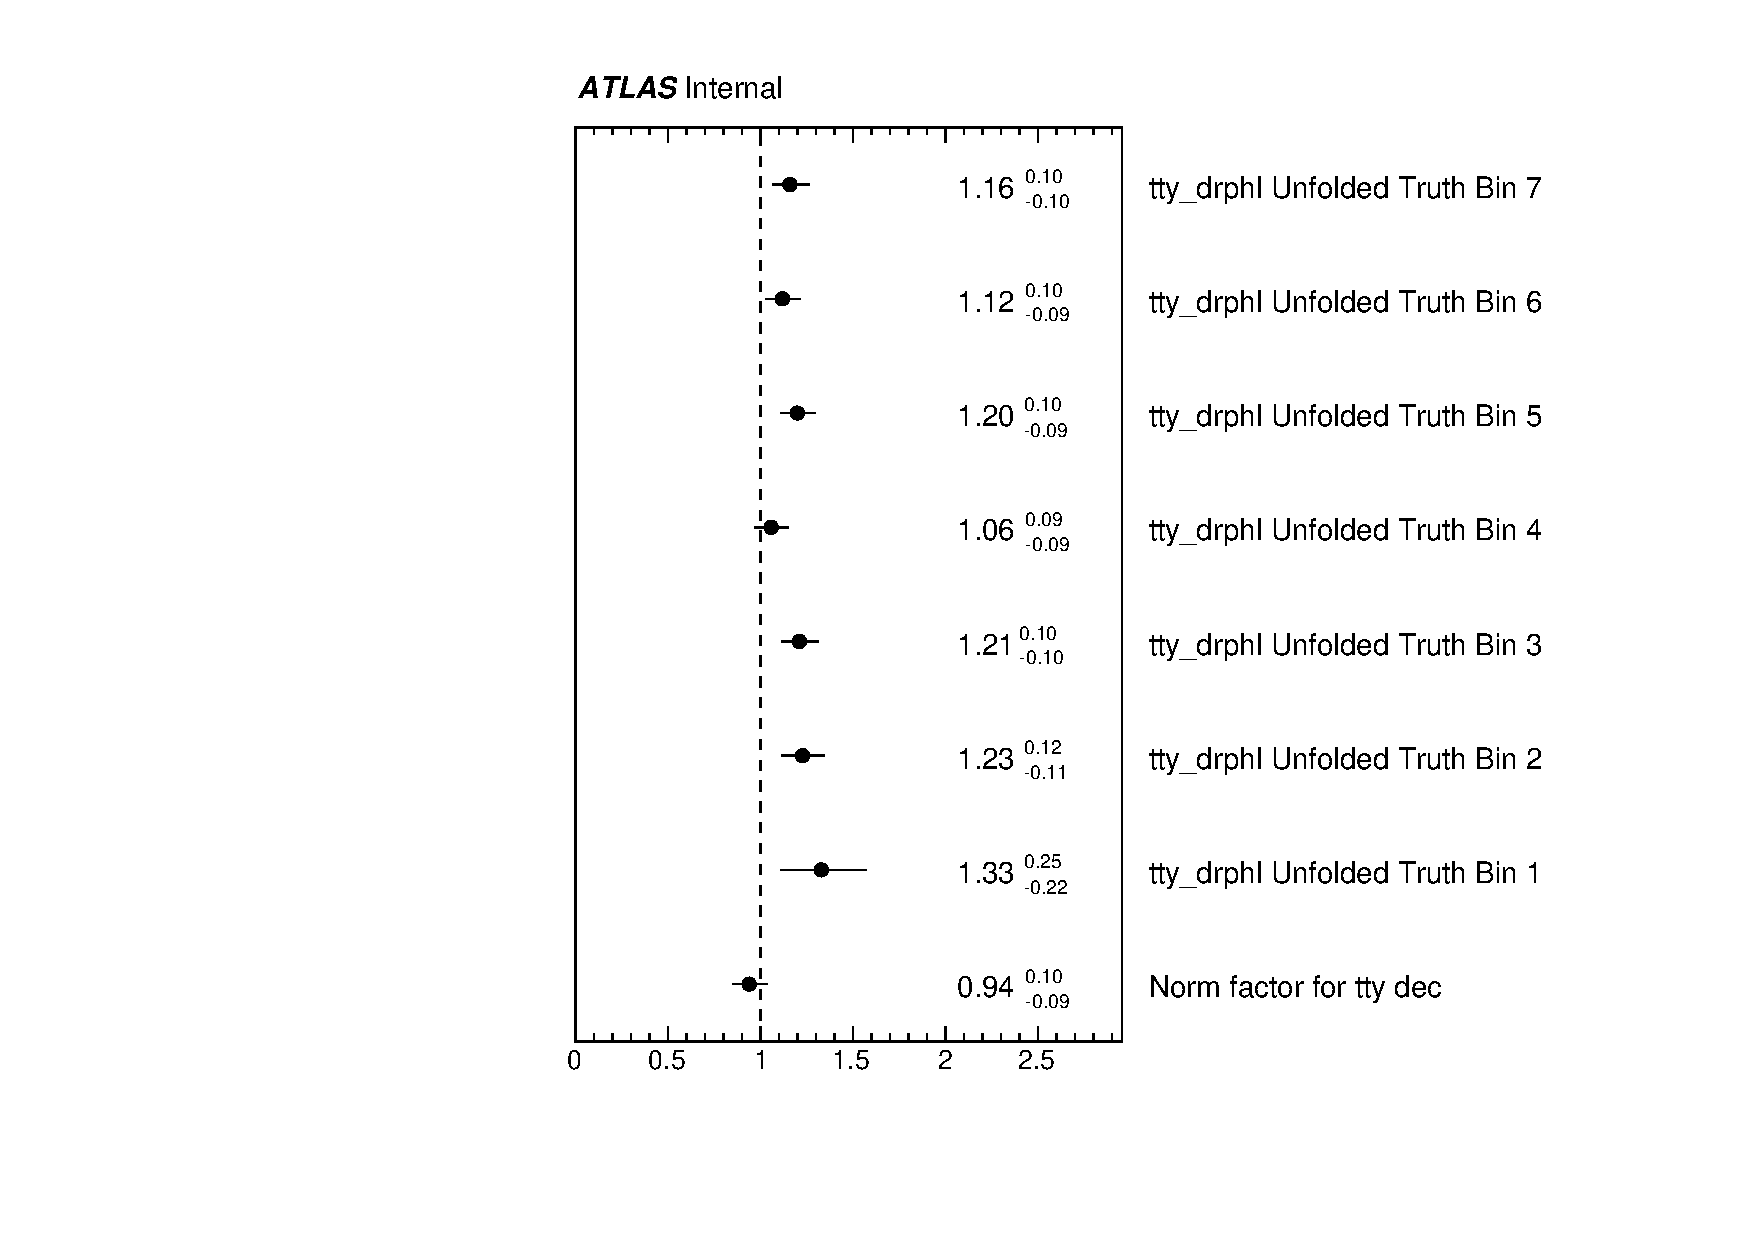
\includegraphics[width=0.3\textwidth]{figures/diff_xsec/ljet_tty_prod_mu_blinded/Unfolded_data/tty1l_dr_all_syst/NormFactors.pdf}}
  \quad
  \subfloat[]{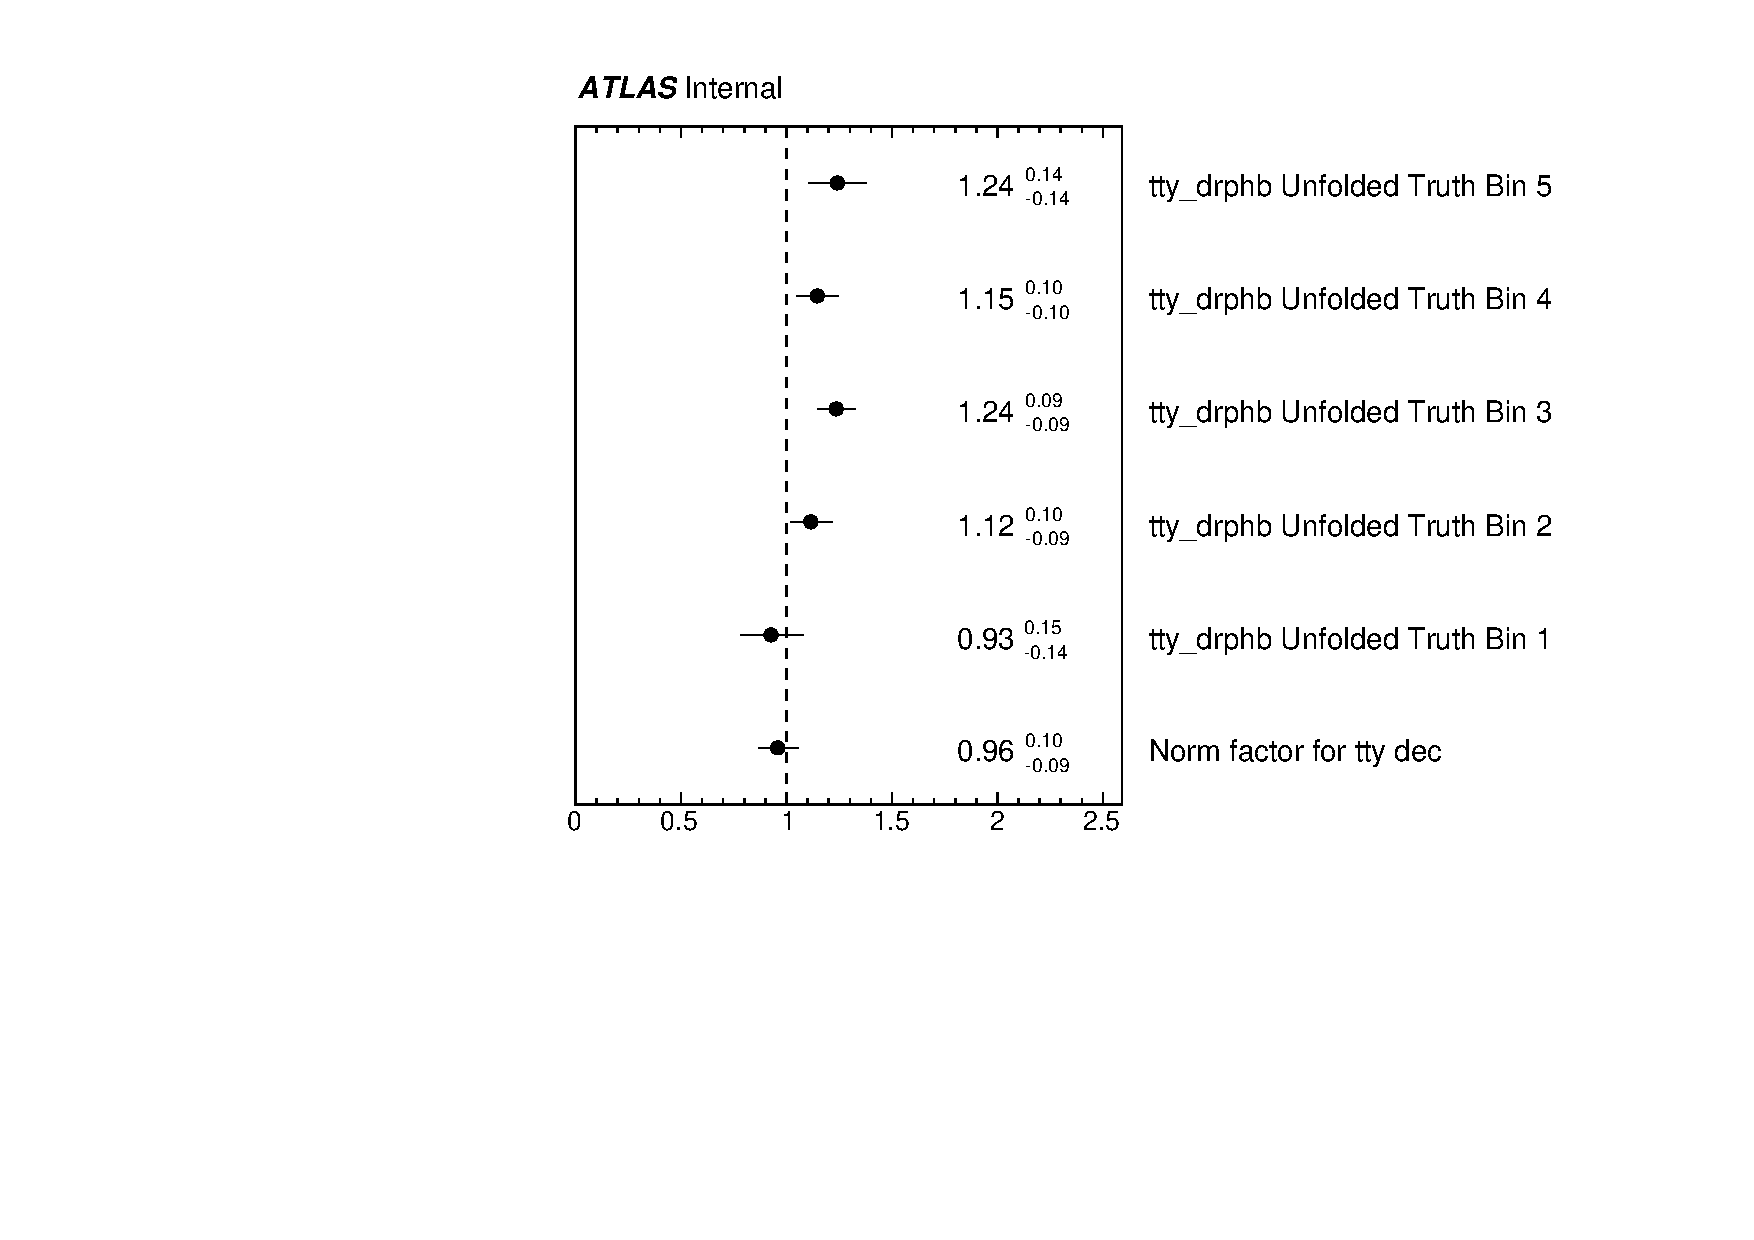
\includegraphics[width=0.3\textwidth]{figures/diff_xsec/ljet_tty_prod_mu_blinded/Unfolded_data/tty1l_drphb_all_syst/NormFactors.pdf}}
  \quad
  \subfloat[]{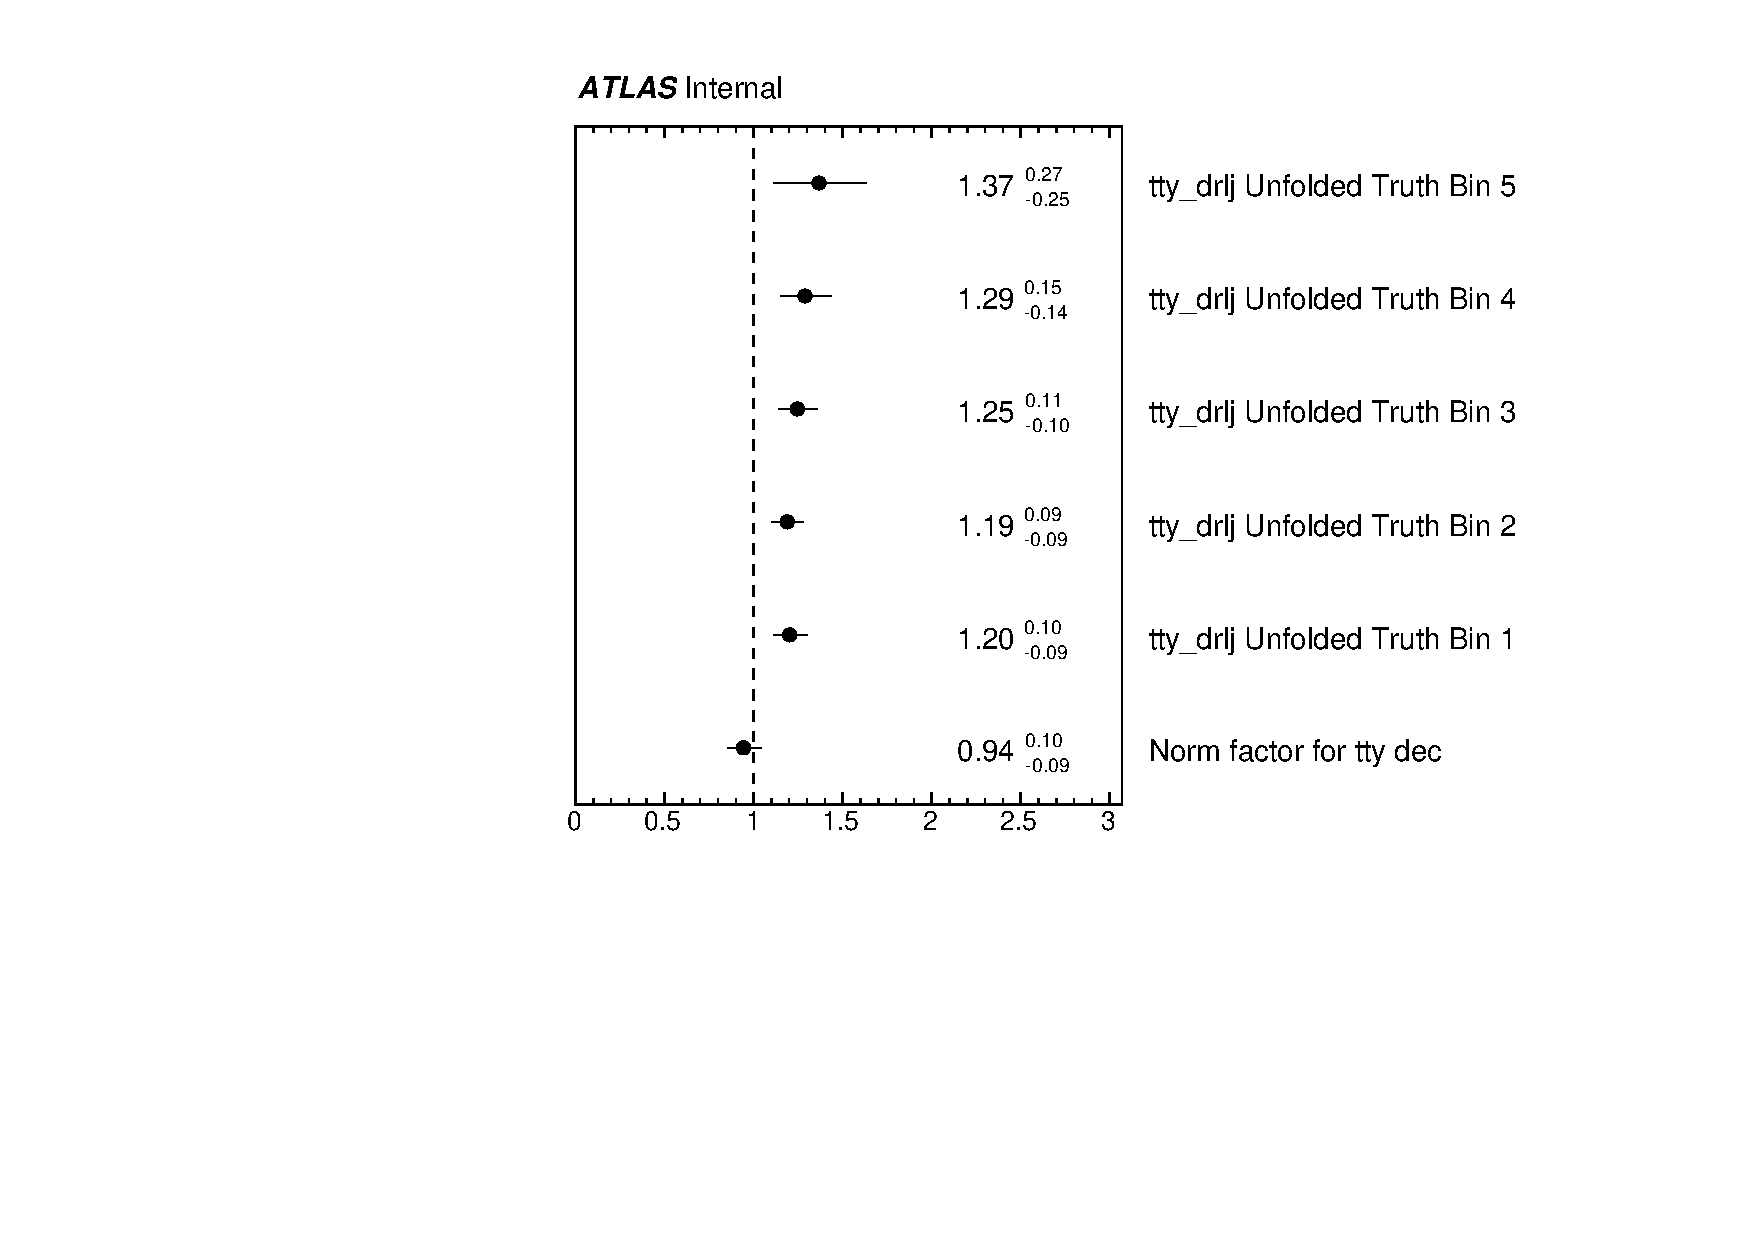
\includegraphics[width=0.3\textwidth]{figures/diff_xsec/ljet_tty_prod_mu_blinded/Unfolded_data/tty1l_drlj_all_syst/NormFactors.pdf}}
  \quad
  \subfloat[]{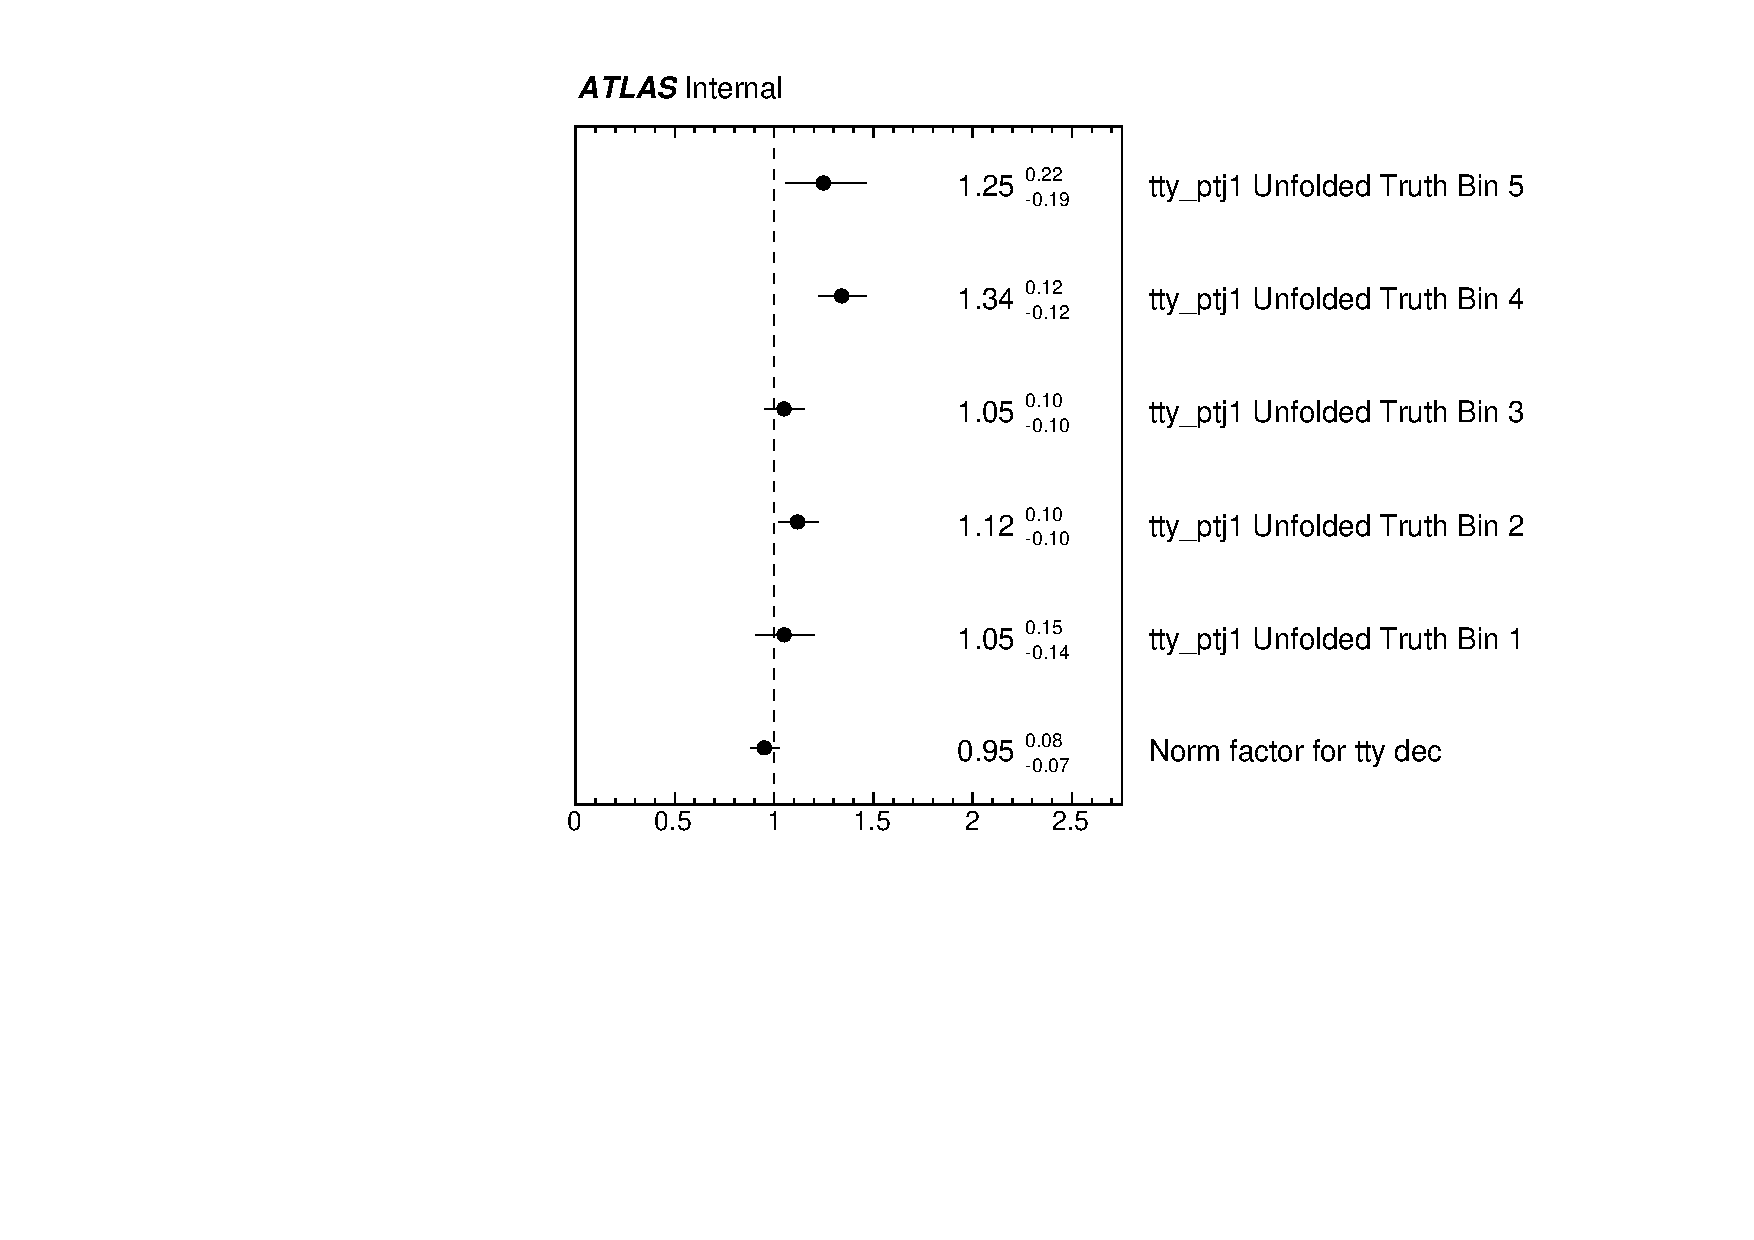
\includegraphics[width=0.3\textwidth]{figures/diff_xsec/ljet_tty_prod_mu_blinded/Unfolded_data/tty1l_ptj1_all_syst/NormFactors.pdf}}
  \caption{ The figure displays the normalization factors obtained from the fit for \tty production measurement in single-lepton channel for the following observables: (a) $p_T(\gamma)$, (b) $|\eta(\gamma|)$, (c) $\Delta R_{min}(\gamma, l)$, (d) $\Delta R(\gamma, b)$, (e) $\Delta R_{min}(l, j)$, (f) $p_T(j1)$.}
  \label{fig:pt_unfolded_ljet_table_realdata}
\end{figure}
\FloatBarrier


\begin{figure}[ht]
  \centering
  \subfloat[]{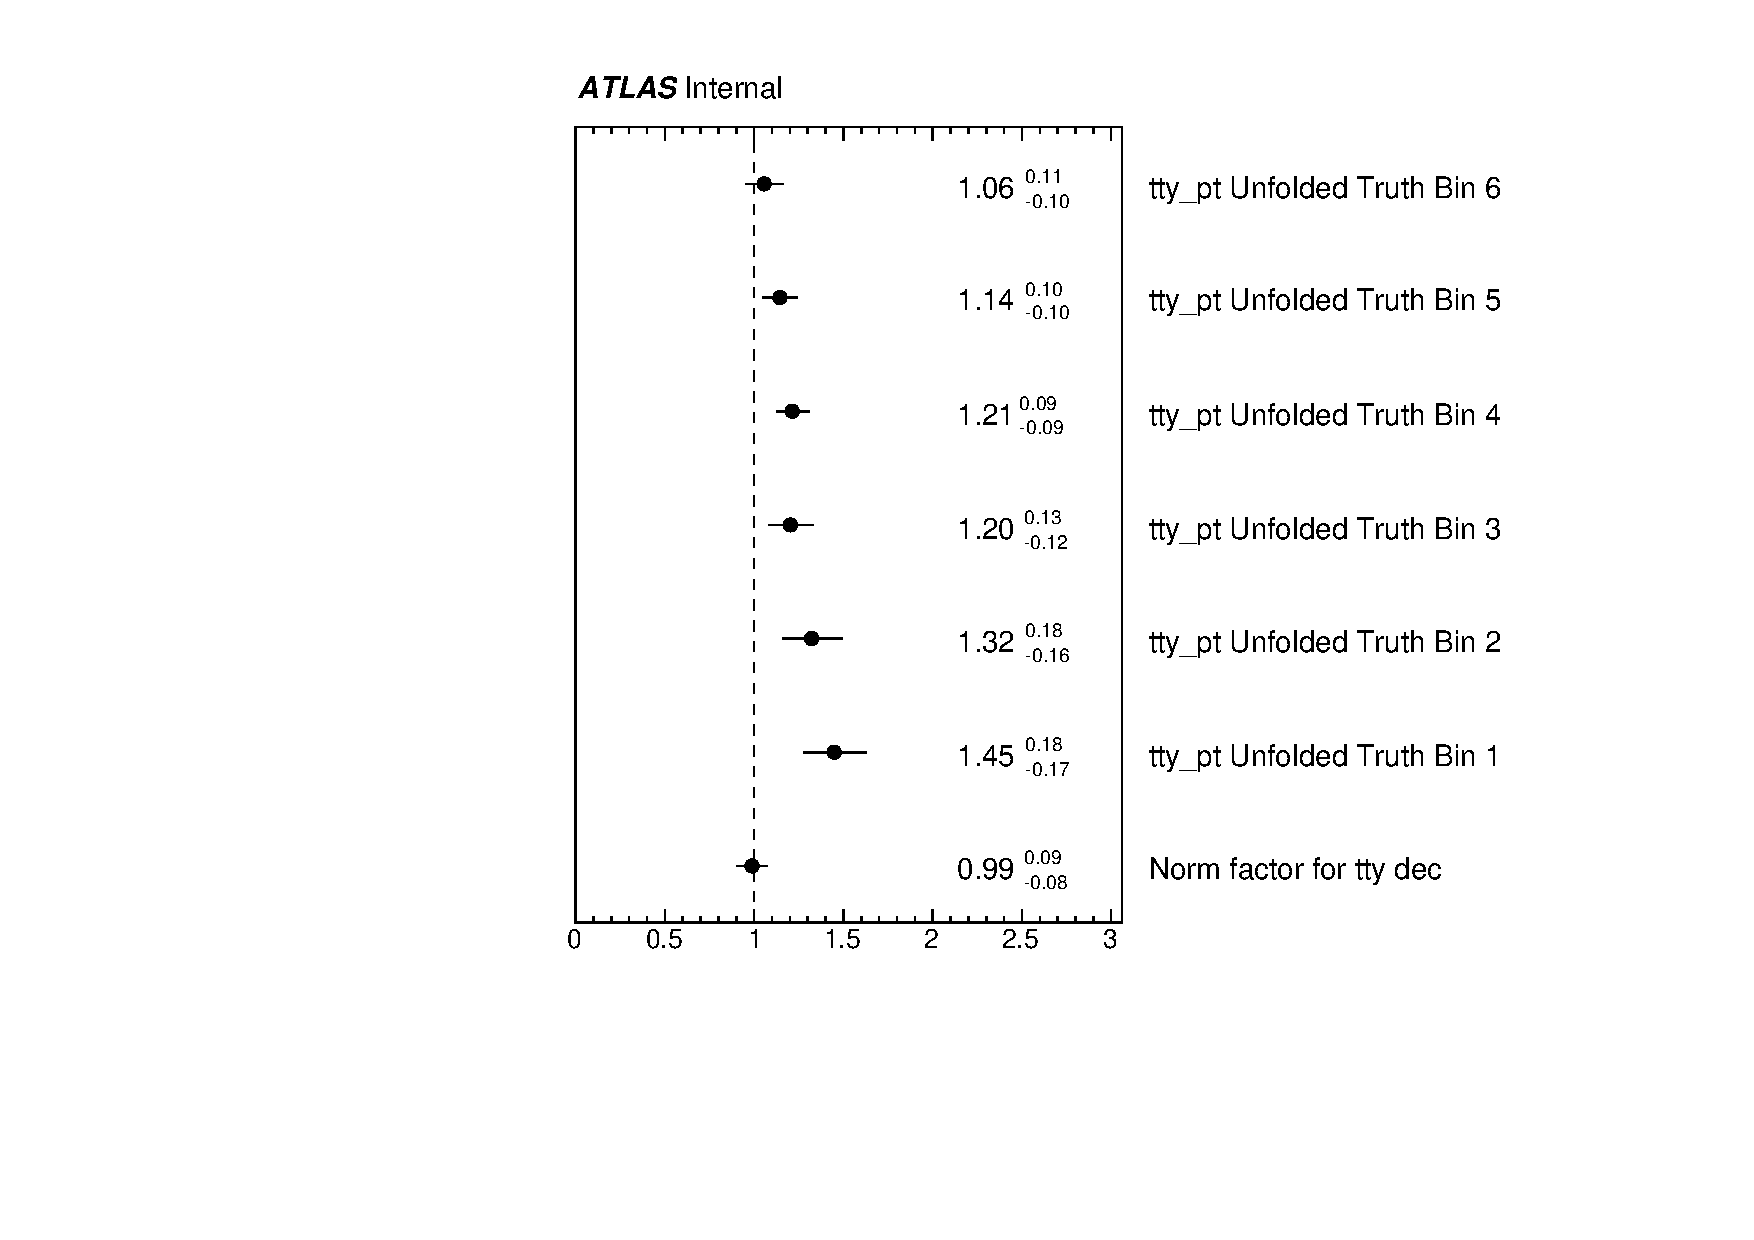
\includegraphics[width=0.3\textwidth]{figures/diff_xsec/dilep_tty_prod_mu_blinded/Unfolded_data/tty2l_pt_all_syst/NormFactors.pdf}}
  \quad
  \subfloat[]{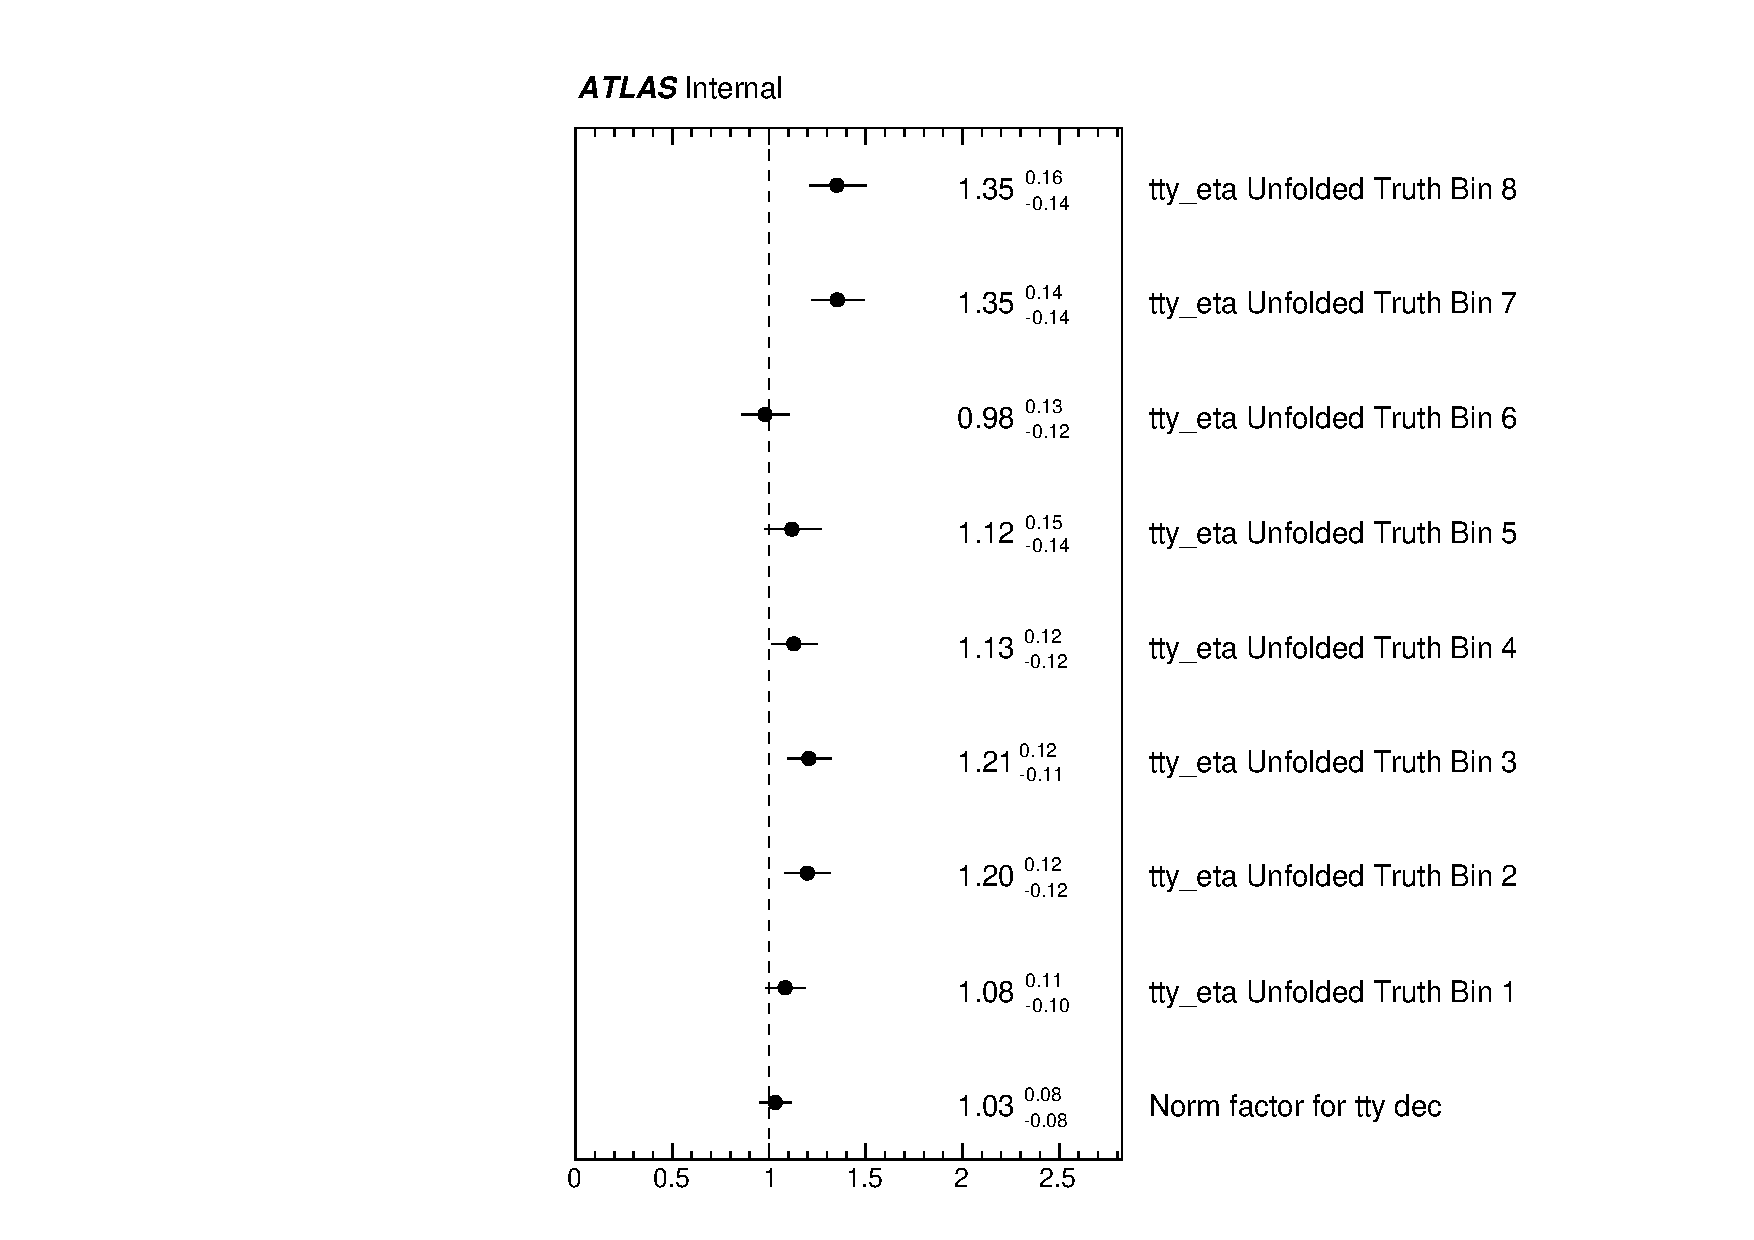
\includegraphics[width=0.3\textwidth]{figures/diff_xsec/dilep_tty_prod_mu_blinded/Unfolded_data/tty2l_eta_all_syst/NormFactors.pdf}}
  \quad
  \subfloat[]{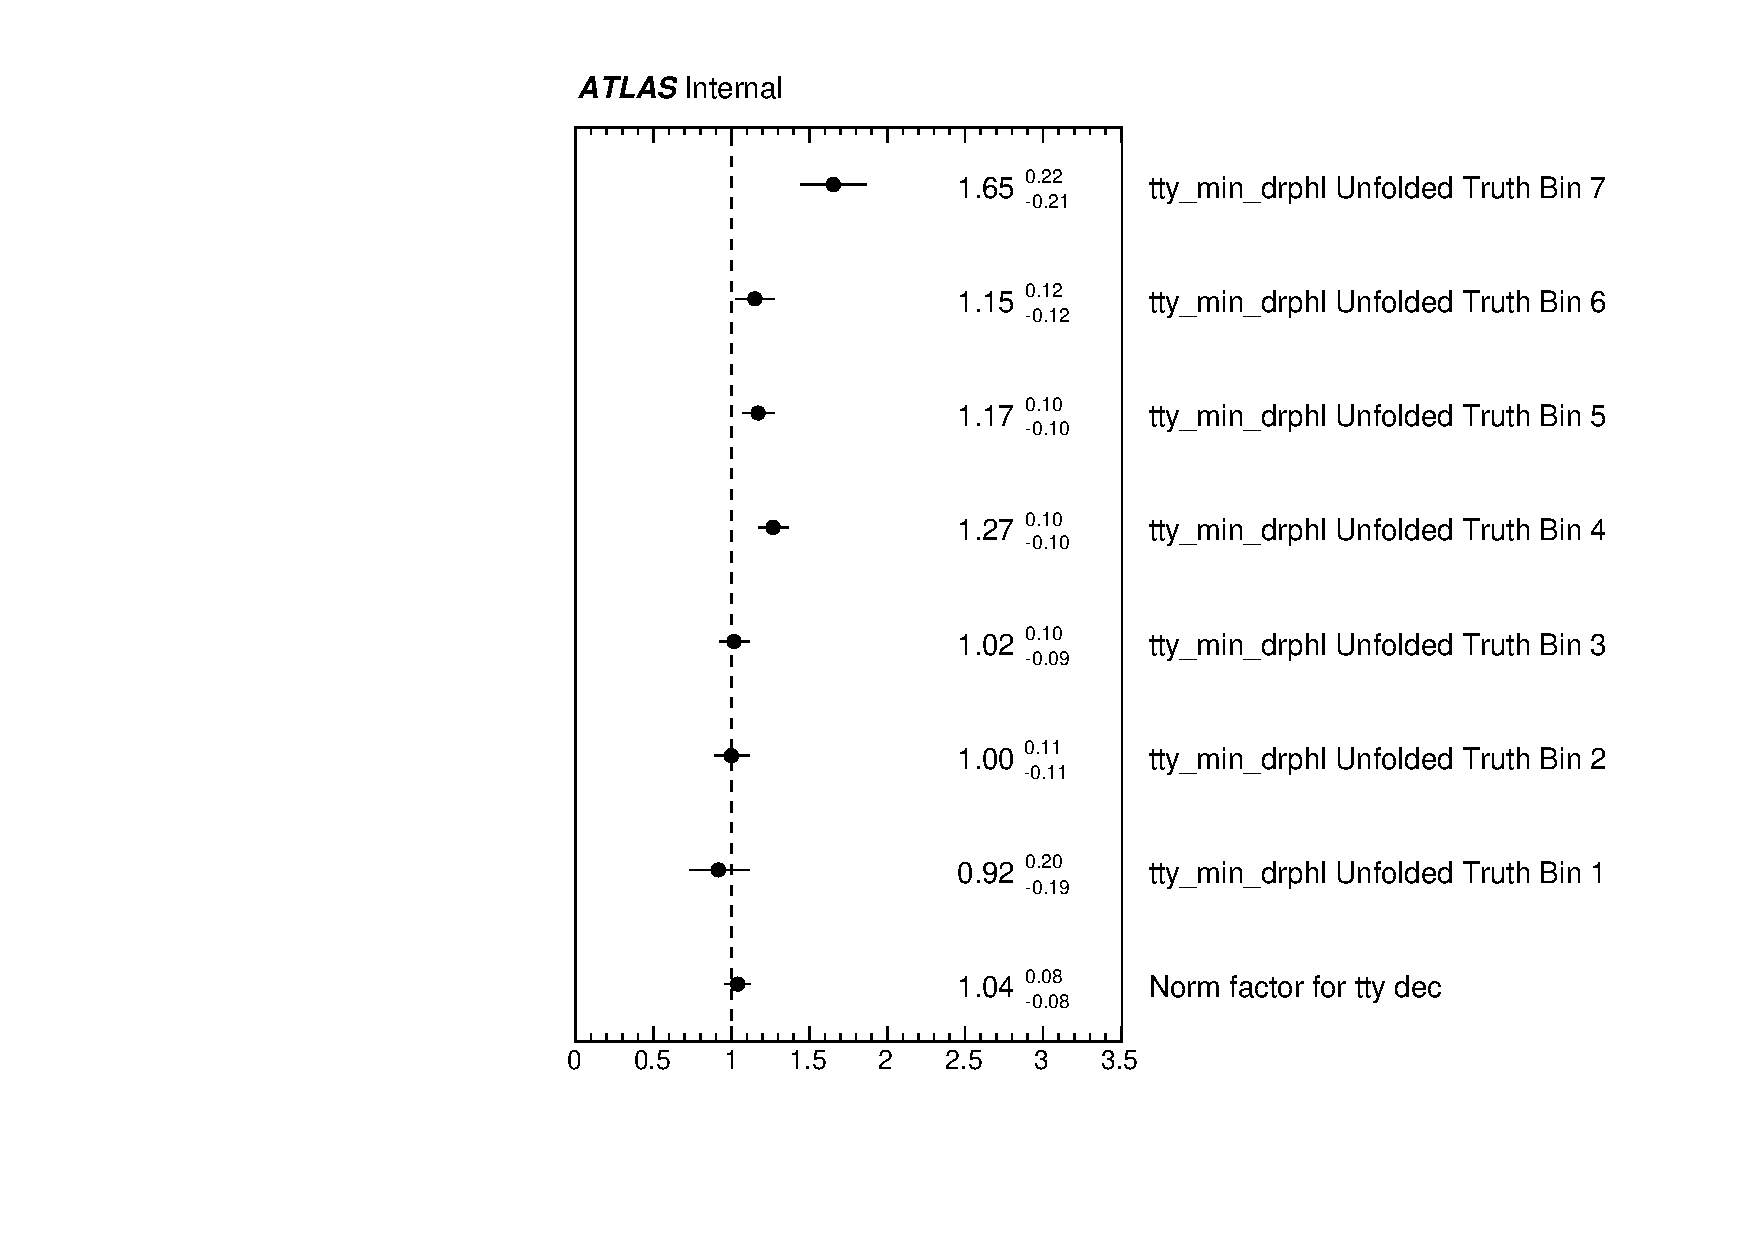
\includegraphics[width=0.3\textwidth]{figures/diff_xsec/dilep_tty_prod_mu_blinded/Unfolded_data/tty2l_dr_all_syst/NormFactors.pdf}}
  \quad
  \subfloat[]{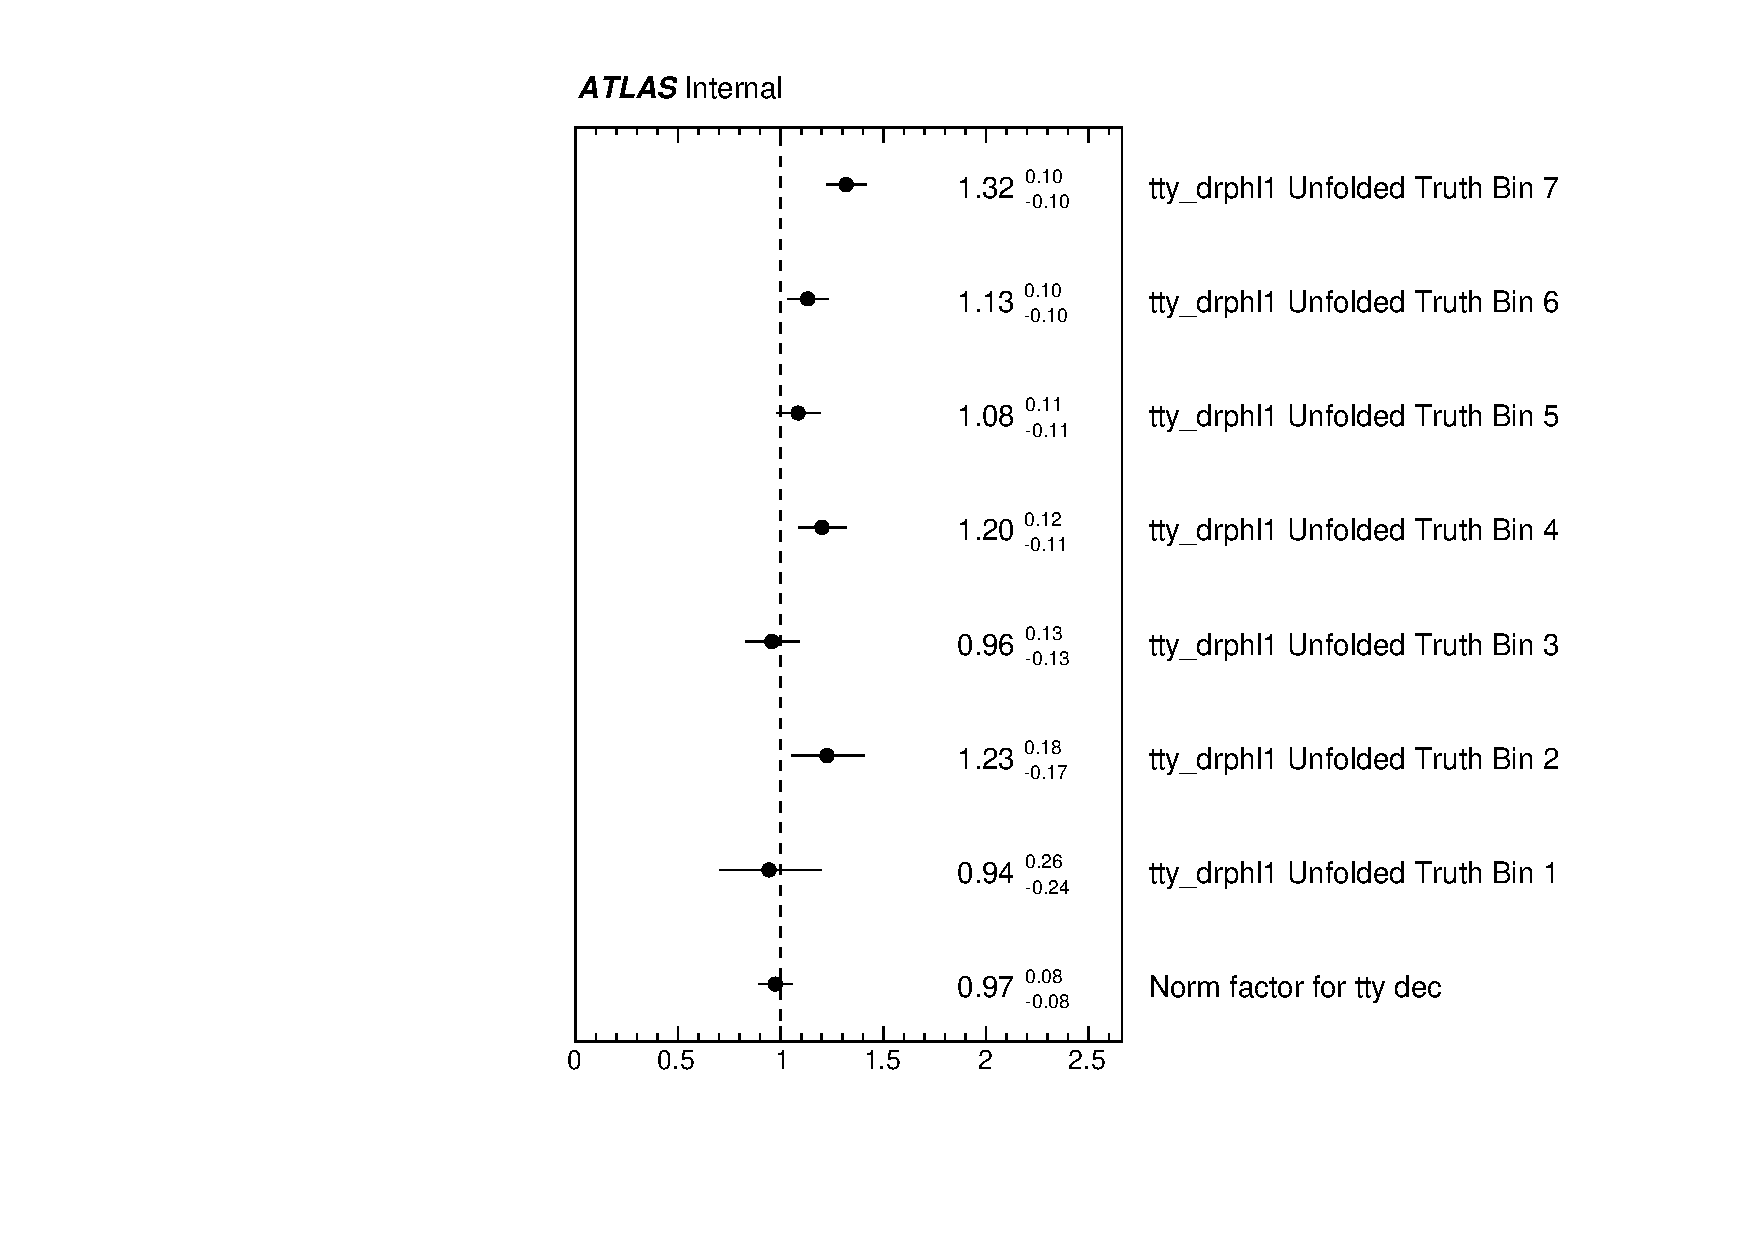
\includegraphics[width=0.3\textwidth]{figures/diff_xsec/dilep_tty_prod_mu_blinded/Unfolded_data/tty2l_dr1_all_syst/NormFactors.pdf}}
  \quad
  \subfloat[]{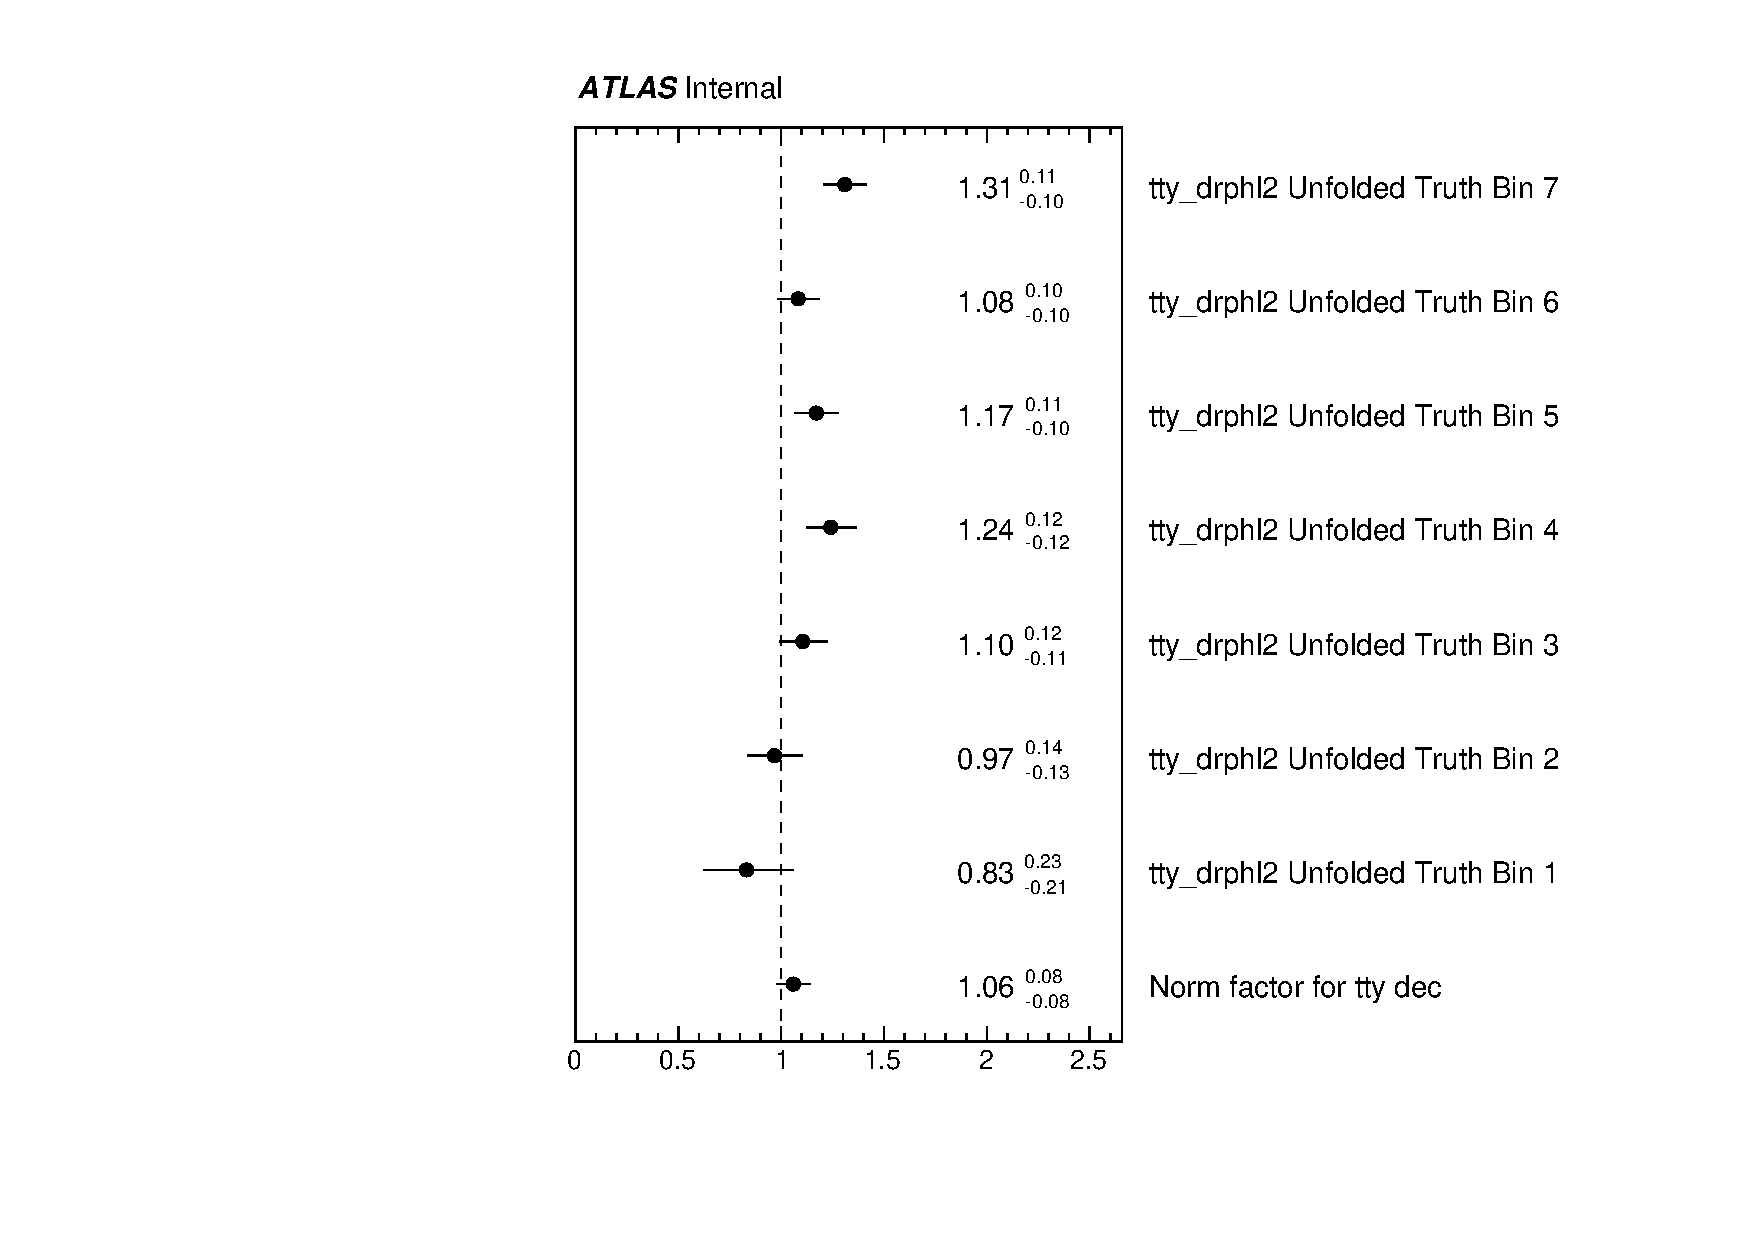
\includegraphics[width=0.3\textwidth]{figures/diff_xsec/dilep_tty_prod_mu_blinded/Unfolded_data/tty2l_dr2_all_syst/NormFactors.pdf}}
  \quad
  \subfloat[]{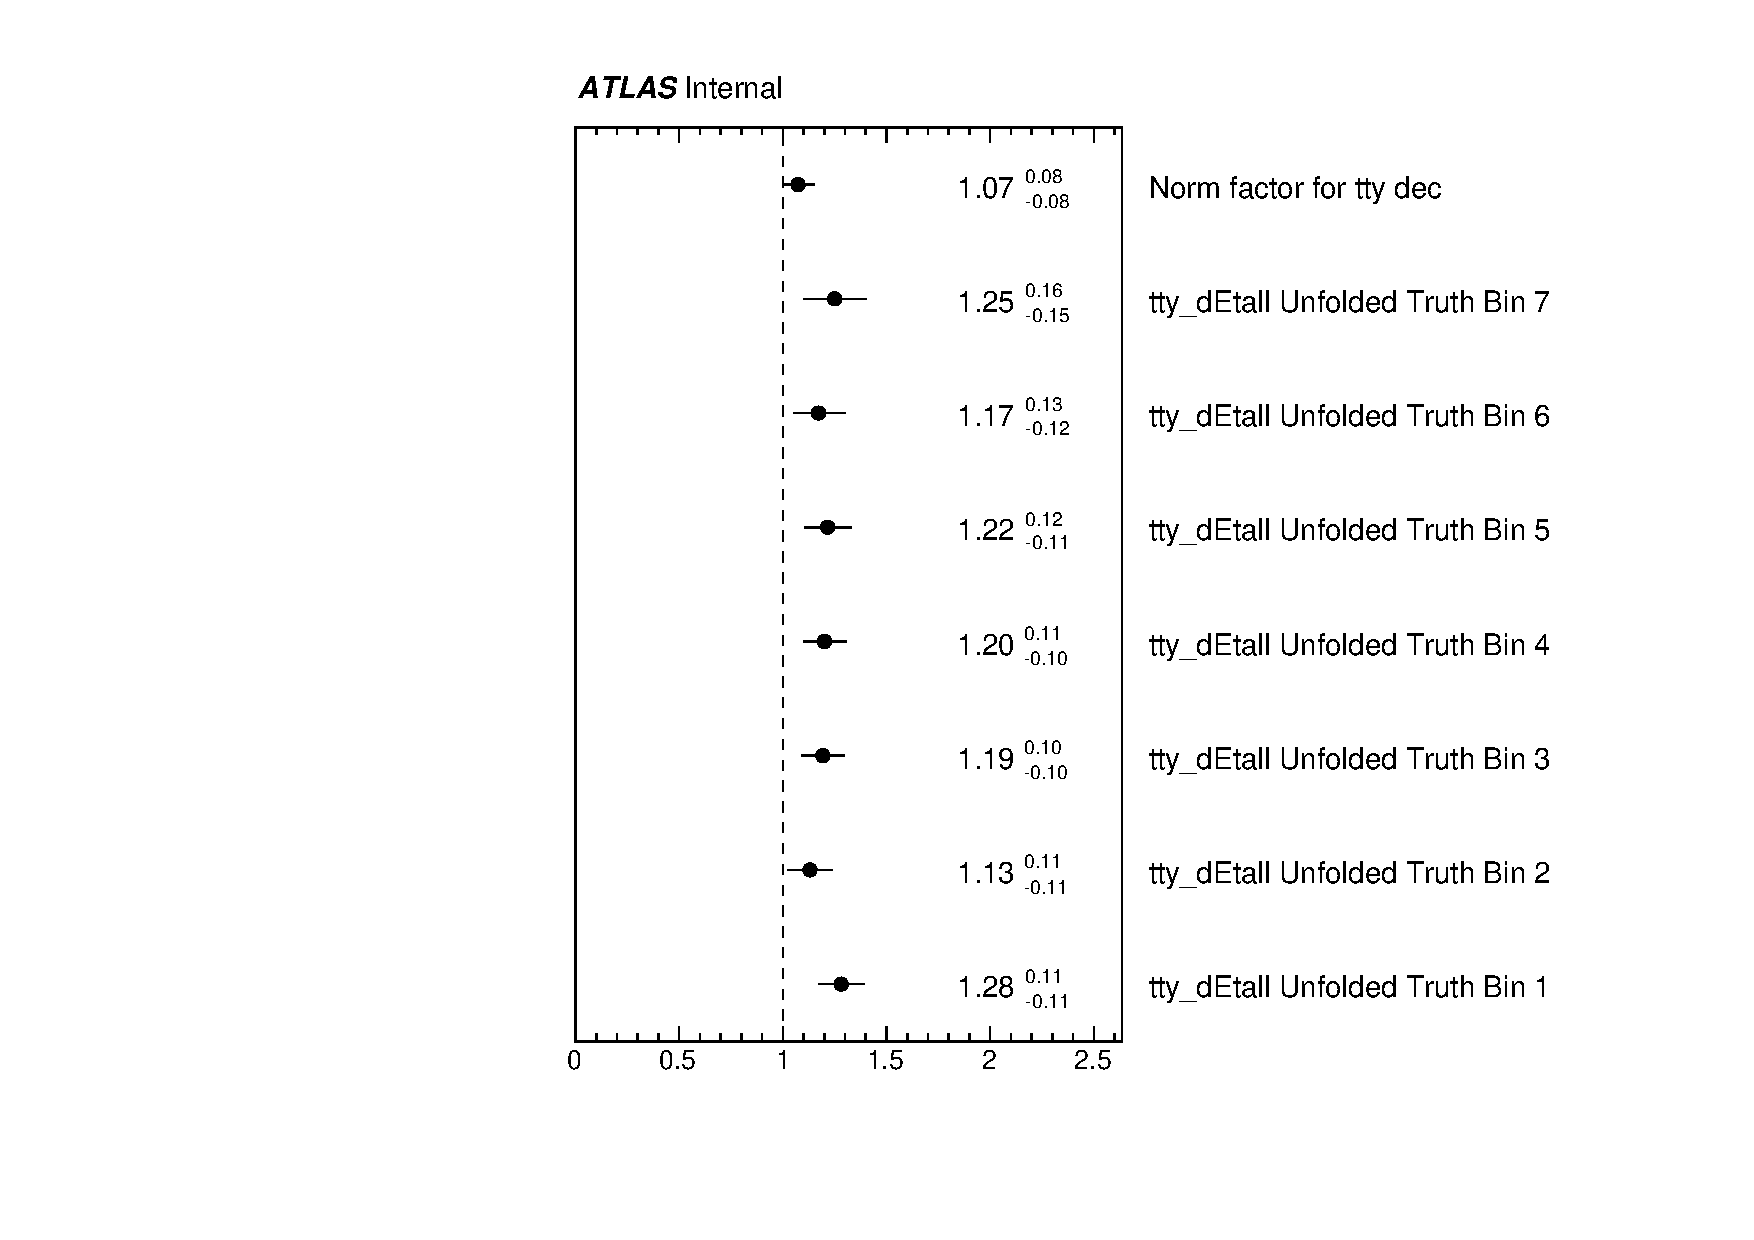
\includegraphics[width=0.3\textwidth]{figures/diff_xsec/dilep_tty_prod_mu_blinded/Unfolded_data/tty2l_dEtall_all_syst/NormFactors.pdf}}
  \quad
  \subfloat[]{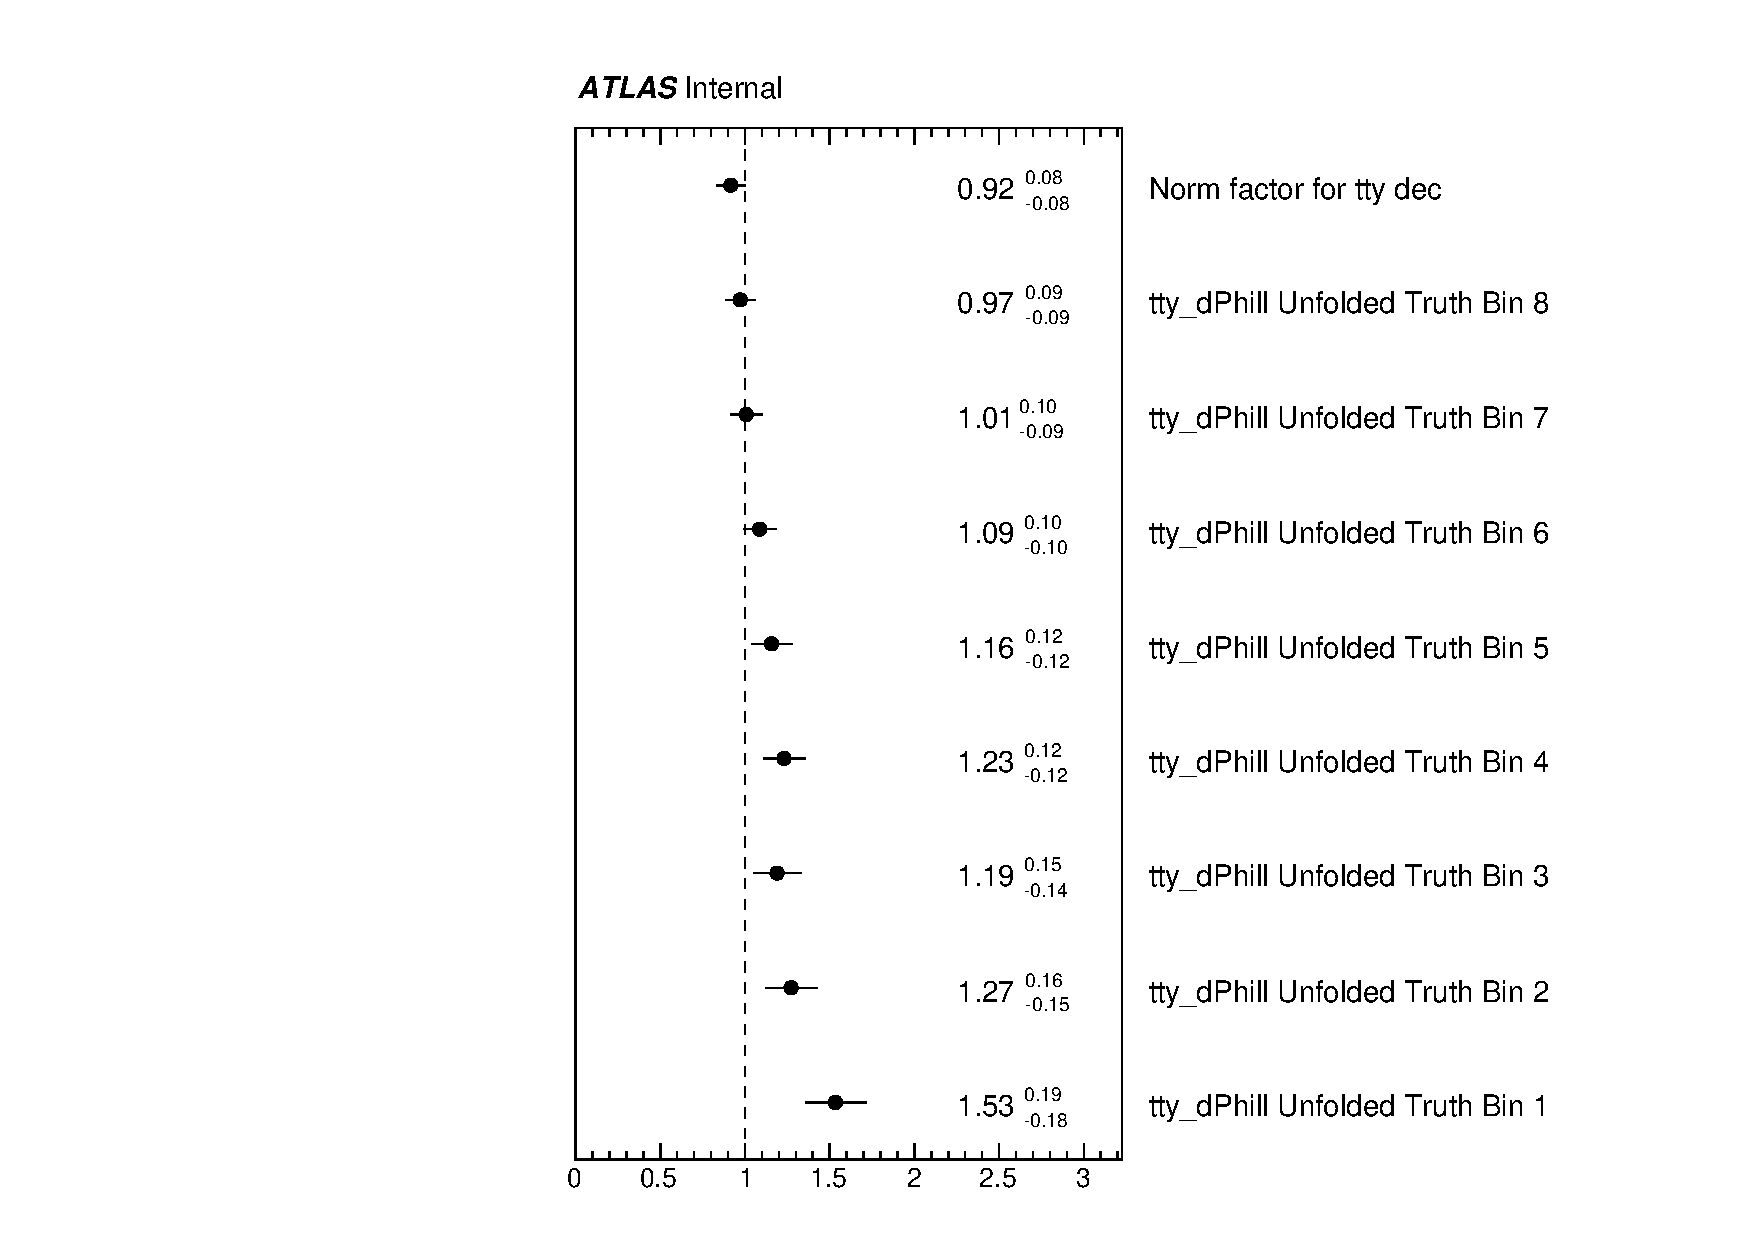
\includegraphics[width=0.3\textwidth]{figures/diff_xsec/dilep_tty_prod_mu_blinded/Unfolded_data/tty2l_dPhill_all_syst/NormFactors.pdf}}
  \quad
  \subfloat[]{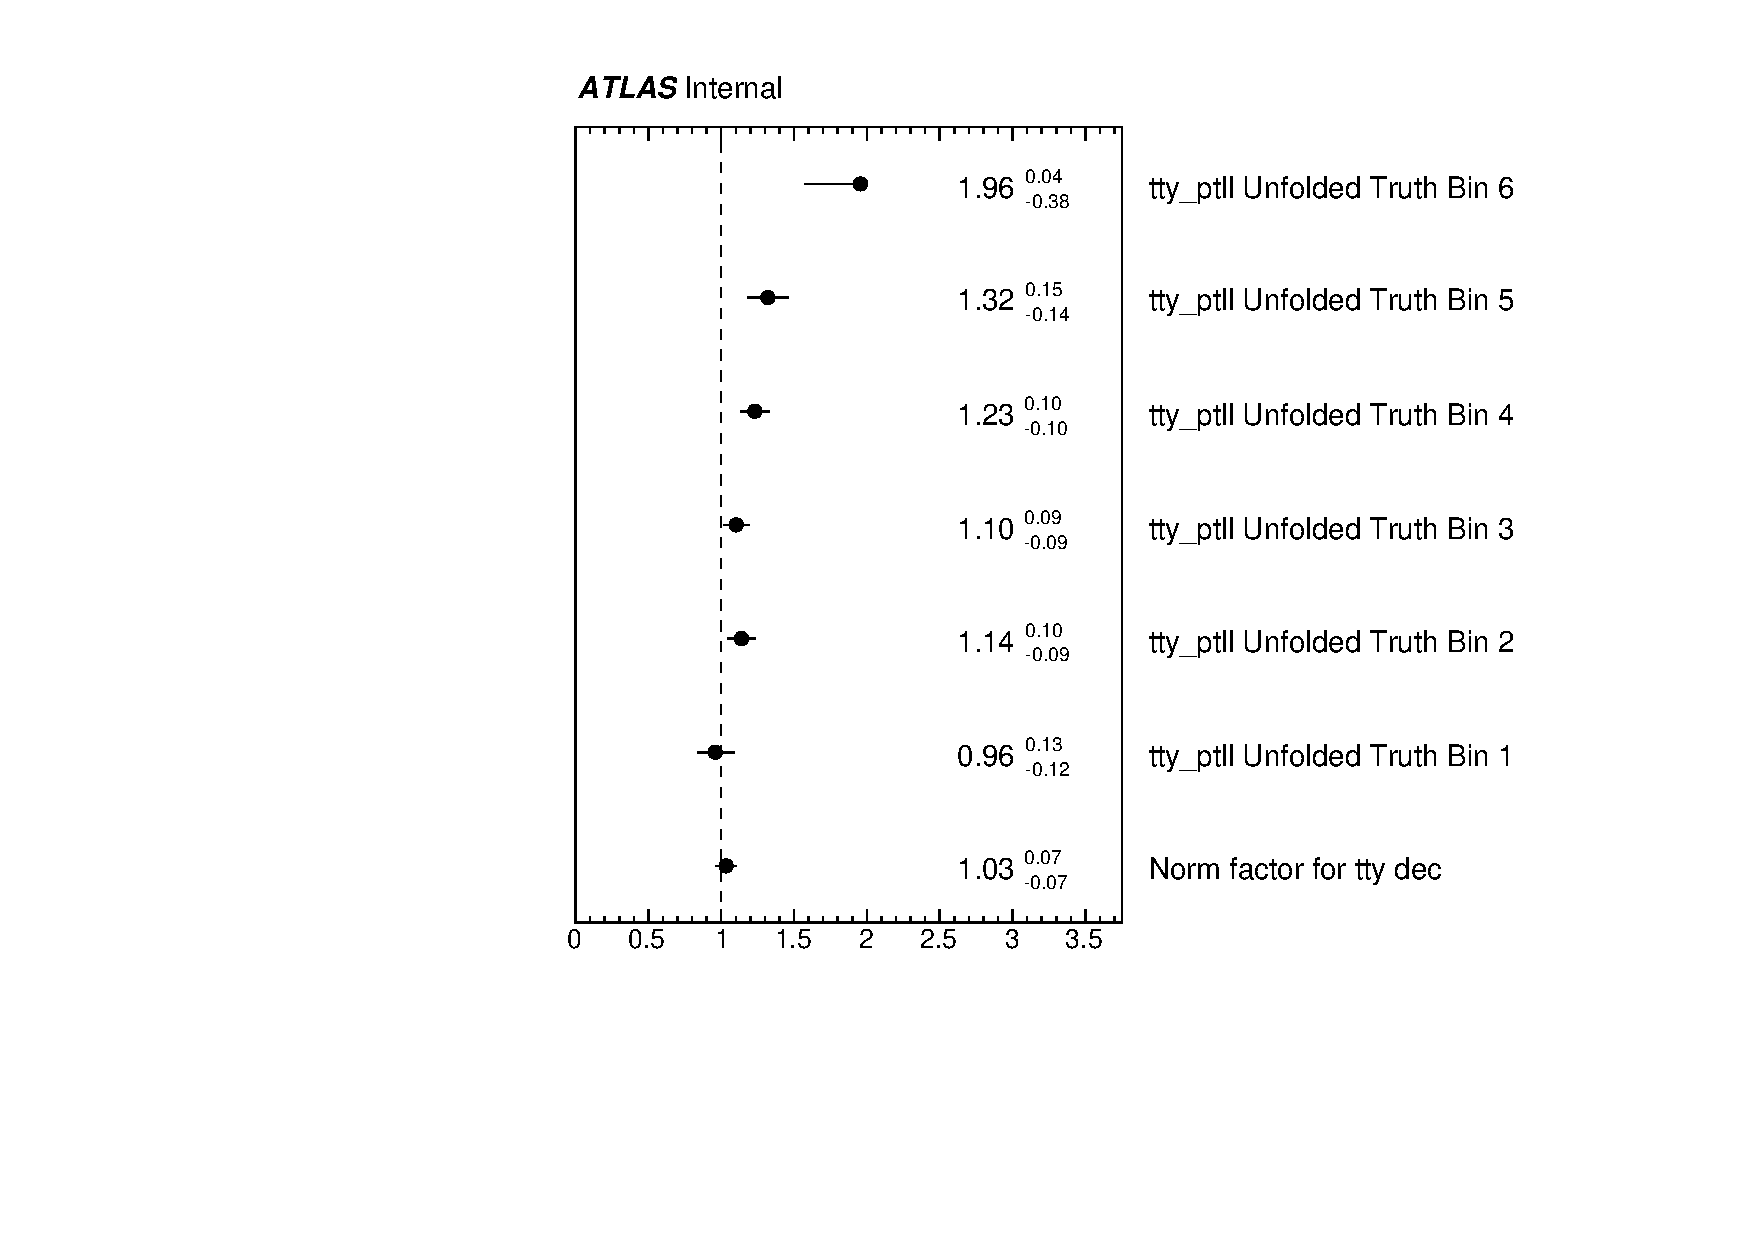
\includegraphics[width=0.3\textwidth]{figures/diff_xsec/dilep_tty_prod_mu_blinded/Unfolded_data/tty2l_ptll_all_syst/NormFactors.pdf}}
  \quad
  \subfloat[]{\includegraphics[width=0.3\textwidth]{figures/diff_xsec/dilep_tty_prod_mu_blinded/Unfolded_data/tty2l_drphb_all_syst/NormFactors.pdf}}
  \quad
  \subfloat[]{\includegraphics[width=0.3\textwidth]{figures/diff_xsec/dilep_tty_prod_mu_blinded/Unfolded_data/tty2l_drlj_all_syst/NormFactors.pdf}}
  \quad
  \subfloat[]{\includegraphics[width=0.3\textwidth]{figures/diff_xsec/dilep_tty_prod_mu_blinded/Unfolded_data/tty2l_ptj1_all_syst/NormFactors.pdf}}
  \caption{ The figure displays the normalisation factors obtained from the fit for \tty production measurement in dilepton channel for the following observables: (a) $p_T(\gamma)$, (b) $|\eta(\gamma|)$, (c) $\Delta R_{min}(\gamma, l)$, (d) $\Delta R(\gamma, l1)$, (e) $\Delta R(\gamma, l2)$, (f) $|\Delta \eta(l, l)|$, (g) $|\Delta \phi(l, l)|$, (h) $p_T(ll)$, (i) $\Delta R(\gamma, b)$, (j) $\Delta R_{min}(l, j)$, (k) $p_T(j1)$.}
  \label{fig:pt_unfolded_dilep_table_realdata}
\end{figure}
\FloatBarrier


\begin{figure}[ht]
  \centering
  \subfloat[]{\includegraphics[width=0.30\textwidth]{figures/diff_xsec/ljet/post_fit/tty1l_pt_all_syst/Plots/SR1_postFit.pdf}}
  \quad \quad
  \subfloat[]{\includegraphics[width=0.30\textwidth]{figures/diff_xsec/ljet/post_fit/tty1l_pt_all_syst/Plots/SR2_postFit.pdf}}
  \quad \quad
  \subfloat[]{\includegraphics[width=0.30\textwidth]{figures/diff_xsec/ljet/post_fit/tty1l_pt_all_syst/Plots/SR3_postFit.pdf}}
  \quad \quad
  \subfloat[]{\includegraphics[width=0.30\textwidth]{figures/diff_xsec/ljet/post_fit/tty1l_pt_all_syst/Plots/SR4_postFit.pdf}}

  \caption{The post-fit distributions of \ptgamma in 4 regions ( (a) \tty production enriched region  (b) \tty decay enriched region (c) fakes enriched region (d) prompt photon enriched region) in single lepton channel. }
  \label{fig:pt_postfit_ljet_realdata}
\end{figure}
\FloatBarrier


\begin{figure}[ht]
  \centering
  \subfloat[]{\includegraphics[width=0.30\textwidth]{figures/diff_xsec/dilep/post_fit/tty2l_pt_all_syst/Plots/SR1_postFit.pdf}}
  \quad \quad
  \subfloat[]{\includegraphics[width=0.30\textwidth]{figures/diff_xsec/dilep/post_fit/tty2l_pt_all_syst/Plots/SR2_postFit.pdf}}
  \caption{The post-fit distributions of \ptgamma in two regions (a) $O_{NN}>=0.6$ (b) $O_{NN}<0.6$ in dilepton channel.}
  \label{fig:pt_postfit_dilep_realdata}
\end{figure}
\FloatBarrier


\begin{figure}[ht]
  \centering
  \subfloat[]{\includegraphics[width=0.40\textwidth, viewport=0 375 150 750, clip]{figures/diff_xsec/ljet_tty_prod_mu_blinded/compare_NP_pulls/compare_NP_dilep_fits_pt_ptj1_eta/NuisPar_comp.pdf}}
  \quad
  \subfloat[]{\includegraphics[width=0.40\textwidth, viewport=0 0 150 375, clip]{figures/diff_xsec/ljet_tty_prod_mu_blinded/compare_NP_pulls/compare_NP_dilep_fits_pt_ptj1_eta/NuisPar_comp.pdf}}
  %\vspace{0.5cm}
  \caption{Pull plots showing pulls and constraints for different observables in single-lepton channel for the \tty production measurement.}
  \label{fig:pull_plot_pt_tty_dec_free_ljet_mu_blinded}
\end{figure}

\begin{figure}[ht]
  \centering
  \subfloat[]{\includegraphics[width=0.40\textwidth, viewport=0 375 150 750, clip]{figures/diff_xsec/ljet_tty_prod_mu_blinded/compare_NP_pulls/compare_NP_dilep_fits_drphb_drlj_dr/NuisPar_comp.pdf}}
  \quad
  \subfloat[]{\includegraphics[width=0.40\textwidth, viewport=0 0 150 375, clip]{figures/diff_xsec/ljet_tty_prod_mu_blinded/compare_NP_pulls/compare_NP_dilep_fits_drphb_drlj_dr/NuisPar_comp.pdf}}
  \caption{Pull plots showing pulls and constraints for different observables in single-lepton channel for the \tty production measurement.}
  \label{fig:pull_plot_pt_tty_dec_free_ljet_mu_blinded}

\end{figure}


\begin{figure}[ht]
  \centering
  \includegraphics[width=0.35\textwidth]{figures/diff_xsec/dilep_tty_prod_mu_blinded/compare_NP_pulls/compare_NP_dilep_fits_pt_ptj1_ptll/NuisPar_comp.pdf}
  \quad \quad 
  \includegraphics[width=0.35\textwidth]{figures/diff_xsec/dilep_tty_prod_mu_blinded/compare_NP_pulls/compare_NP_dilep_fits_dr_dr1_dr2/NuisPar_comp.pdf}
  %\includegraphics[width=0.32\textwidth]{figures/diff_xsec/dilep/Unfolded_data_tty_dec_free_mu_blinded/compare_NP_dilep_fits_pt_ptj1_ptll/NuisPar_Theory.pdf}
  \caption{Pull plots showing pulls and constraints for different observables in dilepton channel for the \tty production measurement.}
  \label{fig:pull_plot_pt_tty_dec_free_dilep_mu_blinded_1}
\end{figure}
\FloatBarrier

\begin{figure}[ht]
  \centering
  \includegraphics[width=0.35\textwidth]{figures/diff_xsec/dilep_tty_prod_mu_blinded/compare_NP_pulls/compare_NP_dilep_fits_detall_dphill_eta/NuisPar_comp.pdf}
  \quad \quad
  \includegraphics[width=0.35\textwidth]{figures/diff_xsec/dilep_tty_prod_mu_blinded/compare_NP_pulls/compare_NP_dilep_fits_drphb_drlj/NuisPar_comp.pdf}
  \caption{Pull plots showing pulls and constraints for different observables in dilepton channel for the \tty production measurement.}
  \label{fig:pull_plot_pt_tty_dec_free_dilep_mu_blinded_2}
\end{figure}
\FloatBarrier



\begin{figure}[ht]
  \centering
  \includegraphics[width=0.8\textwidth]{figures/diff_xsec/ljet_tty_prod_mu_blinded/correlations/tty1l_pt_all_syst/CorrMatrix.pdf}
  \caption{The correlation among NPs and POIs for the measurement of the \ptgamma distribution in single-lepton channel for the \tty production measurement.}
  \label{fig:NP_corr_ljet_mu_blinded}
\end{figure}
\FloatBarrier


\begin{figure}[ht]
  \centering
  \includegraphics[width=0.8\textwidth]{figures/diff_xsec/dilep_tty_prod_mu_blinded/correlations/tty2l_pt_all_syst/CorrMatrix.pdf}
  \caption{The correlation among NPs and POIs for the measurement of the \ptgamma distribution in dilepton channel for the \tty production measurement.}
  \label{fig:NP_corr_dilep_mu_blinded}
\end{figure}
\FloatBarrier

%%%%%%%%%%%% RANKING %%%%%%%%%%%%%%%%%%%

\begin{figure}[ht]
  \centering
  \subfloat[]{\includegraphics[width=0.2\textwidth]{figures/diff_xsec/ljet_tty_prod_mu_blinded/Ranking/tty1l_pt_all_syst/Ranking_tty_pt_Bin_001_mu.pdf}}
  \quad
  \subfloat[]{\includegraphics[width=0.2\textwidth]{figures/diff_xsec/ljet_tty_prod_mu_blinded/Ranking/tty1l_pt_all_syst/Ranking_tty_pt_Bin_002_mu.pdf}}
  \quad
  \subfloat[]{\includegraphics[width=0.2\textwidth]{figures/diff_xsec/ljet_tty_prod_mu_blinded/Ranking/tty1l_pt_all_syst/Ranking_tty_pt_Bin_003_mu.pdf}}
  \quad
  \subfloat[]{\includegraphics[width=0.2\textwidth]{figures/diff_xsec/ljet_tty_prod_mu_blinded/Ranking/tty1l_pt_all_syst/Ranking_tty_pt_Bin_004_mu.pdf}}
  \quad
  \subfloat[]{\includegraphics[width=0.2\textwidth]{figures/diff_xsec/ljet_tty_prod_mu_blinded/Ranking/tty1l_pt_all_syst/Ranking_tty_pt_Bin_005_mu.pdf}}
  \quad
  \subfloat[]{\includegraphics[width=0.2\textwidth]{figures/diff_xsec/ljet_tty_prod_mu_blinded/Ranking/tty1l_pt_all_syst/Ranking_tty_pt_Bin_006_mu.pdf}}
  \quad
  \subfloat[]{\includegraphics[width=0.2\textwidth]{figures/diff_xsec/ljet_tty_prod_mu_blinded/Ranking/tty1l_pt_all_syst/Ranking_tty_pt_Bin_007_mu.pdf}}
  \quad
  \subfloat[]{\includegraphics[width=0.2\textwidth]{figures/diff_xsec/ljet_tty_prod_mu_blinded/Ranking/tty1l_pt_all_syst/Ranking_tty_pt_Bin_008_mu.pdf}}
  \quad
  \subfloat[]{\includegraphics[width=0.2\textwidth]{figures/diff_xsec/ljet_tty_prod_mu_blinded/Ranking/tty1l_pt_all_syst/Ranking_tty_pt_Bin_009_mu.pdf}}
  \quad
  \subfloat[]{\includegraphics[width=0.2\textwidth]{figures/diff_xsec/ljet_tty_prod_mu_blinded/Ranking/tty1l_pt_all_syst/Ranking_tty_pt_Bin_010_mu.pdf}}
  \quad

  \caption{Ranking plots showing the 10 NPs with the largest impact on the \tty production signal strength in each bin of the \ptgamma distribution in the single-lepton channel. Each subfigure, labeled (a), (b), (c), (d), ... (j), corresponds to a specific bin of the \ptgamma distribution, with bin 1 represented in subfigure (a), bin 2 represented in subfigure (b), and so on.}
  \label{fig:ranking_ljet_prod}
\end{figure}
\FloatBarrier


\begin{figure}[ht]
  \centering
  \subfloat[]{\includegraphics[width=0.2\textwidth]{figures/diff_xsec/dilep_tty_prod_mu_blinded/Ranking/tty2l_pt_all_syst/Ranking_tty_pt_Bin_001_mu.pdf}}
  \quad
  \subfloat[]{\includegraphics[width=0.2\textwidth]{figures/diff_xsec/dilep_tty_prod_mu_blinded/Ranking/tty2l_pt_all_syst/Ranking_tty_pt_Bin_002_mu.pdf}}
  \quad
  \subfloat[]{\includegraphics[width=0.2\textwidth]{figures/diff_xsec/dilep_tty_prod_mu_blinded/Ranking/tty2l_pt_all_syst/Ranking_tty_pt_Bin_003_mu.pdf}}
  \quad
  \subfloat[]{\includegraphics[width=0.2\textwidth]{figures/diff_xsec/dilep_tty_prod_mu_blinded/Ranking/tty2l_pt_all_syst/Ranking_tty_pt_Bin_004_mu.pdf}}
  \quad
  \subfloat[]{\includegraphics[width=0.2\textwidth]{figures/diff_xsec/dilep_tty_prod_mu_blinded/Ranking/tty2l_pt_all_syst/Ranking_tty_pt_Bin_005_mu.pdf}}
  \quad
  \subfloat[]{\includegraphics[width=0.2\textwidth]{figures/diff_xsec/dilep_tty_prod_mu_blinded/Ranking/tty2l_pt_all_syst/Ranking_tty_pt_Bin_006_mu.pdf}}
  \caption{Ranking plots showing the 10 NPs with the largest impact on the \tty production signal strength in each bin of the \ptgamma distribution in the dilepton channel. Each subfigure, labeled (a), (b), (c), (d), ... (j), corresponds to a specific bin of the \ptgamma distribution, with bin 1 represented in subfigure (a), bin 2 represented in subfigure (b), and so on.}
  \label{fig:ranking_dilep_prod}
\end{figure}
\FloatBarrier

\begin{figure}[ht]
  \centering
  \subfloat[]{\includegraphics[width=0.4\textwidth]{figures/diff_xsec/absolute-unfolded-distributions/tty_prod_ljet/SL_tty_prod_pt_unfolded_absolute.pdf}}
  \quad\quad
  \subfloat[]{\includegraphics[width=0.4\textwidth]{figures/diff_xsec/absolute-unfolded-distributions/tty_prod_ljet/SL_tty_prod_eta_unfolded_absolute.pdf}}
  \quad\quad
  \subfloat[]{\includegraphics[width=0.4\textwidth]{figures/diff_xsec/absolute-unfolded-distributions/tty_prod_ljet/SL_tty_prod_drphl_unfolded_absolute.pdf}}
  \quad\quad
  \subfloat[]{\includegraphics[width=0.4\textwidth]{figures/diff_xsec/absolute-unfolded-distributions/tty_prod_ljet/SL_tty_prod_drphb_unfolded_absolute.pdf}}
  \quad\quad
  \subfloat[]{\includegraphics[width=0.4\textwidth]{figures/diff_xsec/absolute-unfolded-distributions/tty_prod_ljet/SL_tty_prod_drlj_unfolded_absolute.pdf}}
  \quad\quad
  \subfloat[]{\includegraphics[width=0.4\textwidth]{figures/diff_xsec/absolute-unfolded-distributions/tty_prod_ljet/SL_tty_prod_ptj1_unfolded_absolute.pdf}}
  \quad\quad
  \caption{Absolute differential cross-sections of \tty production in single-lepton fiducial phase space as a function of several observables. Data are compared with \madgraph simulation interfaced with \pythia and \herwig. The last bin includes overflow events.}
  \label{fig:pt_unfolded_ljet_dist_realdata}
\end{figure}
\FloatBarrier



\begin{figure}[ht]
  \centering
  \subfloat[]{\includegraphics[width=0.4\textwidth]{figures/diff_xsec/absolute-unfolded-distributions/tty_prod_dilep/DL_tty_prod_pt_unfolded_absolute.pdf}}
  \quad\quad
  \subfloat[]{\includegraphics[width=0.4\textwidth]{figures/diff_xsec/absolute-unfolded-distributions/tty_prod_dilep/DL_tty_prod_eta_unfolded_absolute.pdf}}
  \quad\quad
  \subfloat[]{\includegraphics[width=0.4\textwidth]{figures/diff_xsec/absolute-unfolded-distributions/tty_prod_dilep/DL_tty_prod_drphl_unfolded_absolute.pdf}}
  \quad\quad
  \subfloat[]{\includegraphics[width=0.4\textwidth]{figures/diff_xsec/absolute-unfolded-distributions/tty_prod_dilep/DL_tty_prod_drphl1_unfolded_absolute.pdf}}
  \quad\quad
  \subfloat[]{\includegraphics[width=0.4\textwidth]{figures/diff_xsec/absolute-unfolded-distributions/tty_prod_dilep/DL_tty_prod_drphl2_unfolded_absolute.pdf}}
  \quad\quad
  \subfloat[]{\includegraphics[width=0.4\textwidth]{figures/diff_xsec/absolute-unfolded-distributions/tty_prod_dilep/DL_tty_prod_dEtall_unfolded_absolute.pdf}}
  \caption{Absolute differential cross-sections of \tty production in dilepton fiducial phase space as a function of several observables. Data are compared with \madgraph simulation interfaced with \pythia and \herwig. The last bin includes overflow events.}
  \label{fig:pt_unfolded_dilep_dist_realdata_1}
\end{figure}

\begin{figure}[ht]
  \centering
  \subfloat[]{\includegraphics[width=0.4\textwidth]{figures/diff_xsec/absolute-unfolded-distributions/tty_prod_dilep/DL_tty_prod_dPhill_unfolded_absolute.pdf}}
  \quad\quad
  \subfloat[]{\includegraphics[width=0.4\textwidth]{figures/diff_xsec/absolute-unfolded-distributions/tty_prod_dilep/DL_tty_prod_ptll_unfolded_absolute.pdf}}
  \quad\quad
  \subfloat[]{\includegraphics[width=0.4\textwidth]{figures/diff_xsec/absolute-unfolded-distributions/tty_prod_dilep/DL_tty_prod_drphb_unfolded_absolute.pdf}}
  \quad\quad
  \subfloat[]{\includegraphics[width=0.4\textwidth]{figures/diff_xsec/absolute-unfolded-distributions/tty_prod_dilep/DL_tty_prod_drlj_unfolded_absolute.pdf}}
  \quad\quad
  \subfloat[]{\includegraphics[width=0.4\textwidth]{figures/diff_xsec/absolute-unfolded-distributions/tty_prod_dilep/DL_tty_prod_ptj1_unfolded_absolute.pdf}}
  \caption{Absolute differential cross-sections of \tty production in dilepton fiducial phase space as a function of several observables. Data are compared with \madgraph simulation interfaced with \pythia and \herwig. The last bin includes overflow events.}
  \label{fig:pt_unfolded_dilep_dist_realdata_2}
\end{figure}
\FloatBarrier

\begin{figure}[ht]
  \centering
  \includegraphics[width=0.33\textwidth]{figures/diff_xsec/normalized-unfolded-distributions/tty_prod_ljet/SL_tty_prod_pt_unfolded_normalized.pdf}%
  \includegraphics[width=0.33\textwidth]{figures/diff_xsec/normalized-unfolded-distributions/tty_prod_ljet/SL_tty_prod_eta_unfolded_normalized.pdf}%
  \includegraphics[width=0.33\textwidth]{figures/diff_xsec/normalized-unfolded-distributions/tty_prod_ljet/SL_tty_prod_drphb_unfolded_normalized.pdf}\\
  \includegraphics[width=0.33\textwidth]{figures/diff_xsec/normalized-unfolded-distributions/tty_prod_ljet/SL_tty_prod_drphl_unfolded_normalized.pdf}%
  \includegraphics[width=0.33\textwidth]{figures/diff_xsec/normalized-unfolded-distributions/tty_prod_ljet/SL_tty_prod_drlj_unfolded_normalized.pdf}%
  \includegraphics[width=0.33\textwidth]{figures/diff_xsec/normalized-unfolded-distributions/tty_prod_ljet/SL_tty_prod_ptj1_unfolded_normalized.pdf}%
  \caption{Normalised differential \tty production cross-section measured in the single-lepton fiducial phase space as a function of several observables. Data are compared with MadGraph5\_aMC@NLO simulation interfaced with \PYTHIA[8] and \HERWIG[7]. The lower parts of each plot show the ratio of the prediction to the data.}
  \label{fig:tty_prod_diff_Ljets_norm}
\end{figure}
\FloatBarrier

\begin{figure}[ht]
  \centering
  \includegraphics[width=0.33\textwidth]{figures/diff_xsec/normalized-unfolded-distributions/tty_prod_dilep/DL_tty_prod_pt_unfolded_normalized.pdf}%
  \includegraphics[width=0.33\textwidth]{figures/diff_xsec/normalized-unfolded-distributions/tty_prod_dilep/DL_tty_prod_eta_unfolded_normalized.pdf}%
  \includegraphics[width=0.33\textwidth]{figures/diff_xsec/normalized-unfolded-distributions/tty_prod_dilep/DL_tty_prod_drphb_unfolded_normalized.pdf}\\
  \includegraphics[width=0.33\textwidth]{figures/diff_xsec/normalized-unfolded-distributions/tty_prod_dilep/DL_tty_prod_drphl_unfolded_normalized.pdf}%
  \includegraphics[width=0.33\textwidth]{figures/diff_xsec/normalized-unfolded-distributions/tty_prod_dilep/DL_tty_prod_drlj_unfolded_normalized.pdf}%
  \caption{Normalised differential \tty production cross-section measured in the dilepton fiducial phase space as a function of several observables. Data are compared with MadGraph5\_aMC@NLO simulation interfaced with \PYTHIA[8] and \HERWIG[7]. The lower parts of each plot show the ratio of the prediction to the data.}
  \label{fig:tty_prod_diff_DL1_norm}
\end{figure}
\FloatBarrier


\begin{figure}[ht]
  \centering
  \includegraphics[width=0.33\textwidth]{figures/diff_xsec/normalized-unfolded-distributions/tty_prod_dilep/DL_tty_prod_ptll_unfolded_normalized.pdf}%
  \includegraphics[width=0.33\textwidth]{figures/diff_xsec/normalized-unfolded-distributions/tty_prod_dilep/DL_tty_prod_dEtall_unfolded_normalized.pdf}%
  \includegraphics[width=0.33\textwidth]{figures/diff_xsec/normalized-unfolded-distributions/tty_prod_dilep/DL_tty_prod_dPhill_unfolded_normalized.pdf}\\
  \includegraphics[width=0.33\textwidth]{figures/diff_xsec/normalized-unfolded-distributions/tty_prod_dilep/DL_tty_prod_drphl1_unfolded_normalized.pdf}%
  \includegraphics[width=0.33\textwidth]{figures/diff_xsec/normalized-unfolded-distributions/tty_prod_dilep/DL_tty_prod_drphl2_unfolded_normalized.pdf}%
  \includegraphics[width=0.33\textwidth]{figures/diff_xsec/normalized-unfolded-distributions/tty_prod_dilep/DL_tty_prod_ptj1_unfolded_normalized.pdf}%
  \caption{Normalised differential \tty production cross-section measured in the dilepton fiducial phase space as a function of several observables. Data are compared with MadGraph5\_aMC@NLO simulation interfaced with \PYTHIA[8] and \HERWIG[7]. The lower parts of each plot show the ratio of the prediction to the data.}
  \label{fig:tty_prod_diff_DL2_norm}
\end{figure}
\FloatBarrier


\begin{table}
  \scriptsize
  \centering
  \caption{$\chi^2$/ndf and $p$-values between the measured absolute and normalised cross-sections of \tty production and the NLO \MGNLO simulations interfaced with \PYTHIA[8] and \HERWIG[7].}
  \scalebox{0.8}{
  \begin{tabular}{l | c c | c c | c c |  c c }
  \toprule
    & \multicolumn{4}{c}{Absolute cross-sections} & \multicolumn{4}{c}{Normalised cross-sections} \\
    &  \multicolumn{2}{c}{MG5\_aMC@NLO+\Pythia[8]} & \multicolumn{2}{c}{MG5\_aMC@NLO+\Herwig[7]} &  \multicolumn{2}{c}{MG5\_aMC@NLO+\Pythia[8]} & \multicolumn{2}{c}{MG5\_aMC@NLO+\Herwig[7]}\\
  Variables & $\chi^2$/ndf & $p$-value & $\chi^2$/ndf & $p$-value & $\chi^2$/ndf & $p$-value & $\chi^2$/ndf & $p$-value \\
  \midrule
  \multicolumn{9}{c}{Single-lepton channel} \\
  \midrule
  \pt($\gamma$) &	 12.3/10&	 0.26&	 11.1/10&	 0.35&	 64.8/9&	 $<0.01$ &	 49.6/9& 	 $<0.01$ \\ 
                  
  $|\eta|$($\gamma$) &	 11.5/8&	 0.18&	 11.0/8&	 0.20&	 8.0/7&	 0.33&	 8.3/7& 	 0.31 \\
                  
  $\Delta R(\gamma, \ell)$ &	 10.2/7&	 0.18&	 9.6/7&	 0.22&	 8.5/6&	 0.2&	 8.5/6& 	 0.21 \\
                  
  $\Delta R(\gamma, b)_{min}$&	 12.4/5&	 0.03&	 12.0/5&	 0.04&	 7.5/4&	 0.11&	 8.7/4& 	 0.07 \\
                  
  $\Delta R(\ell, j)_{min}$ &	 6.1/5&	 0.3&	 6.4/5&	 0.27&	 1.5/4&	 0.83&	 2.5/4& 	 0.64 \\
                  
  $\pt(j_1)$ &	 12.0/5&	 0.04&	 10.5/5&	 0.06&	 8.1/4&	 0.09&	 9.7/4& 	 0.05 \\		
  \midrule
  \multicolumn{9}{c}{Dilepton channel} \\
  \midrule
  \pt($\gamma$) &	 8.4/6 &	 0.21 &	 7.0/6 &	 0.32 &	 6.3/5 &	 0.28 &	 5.3/5 & 	 0.38 \\							
  $|\eta|$($\gamma$) &	 12.2/8 &	 0.14 &	 9.9/8 &	 0.27 &	 9.2/7 &	 0.24 &	 7.8/7 & 	 0.35 \\								
  $\Delta R(\gamma, \ell)_{min}$ &	 17.6/7 &	 0.01 &	 17.2/7 &	 0.02 &	 14.2/6 &	 0.03 &	 14.7/6 & 	 0.02 \\ 														
  $\Delta R(\gamma, b)_{min}$ &	 7.7/5 &	 0.17 &	 5.0/5 &	 0.41 &	 1.4/4 &	 0.84 &	 0.8/4 & 	 0.93 \\ 								
  $\Delta R(\ell, j)_{min}$ &	 13.6/5 &	 0.02 &	 9.7/5 &	 0.08 &	 5.3/4 &	 0.26 &	 3.7/4 & 	 0.44 \\ 								
  $\pt(j_1)$ &	 10.2/5 &	 0.07 &	 4.9/5 &	 0.42 &	 7.8/4 &	 0.1 &	 3.6/4 & 	 0.46 \\
  $\Delta R(\gamma, \ell_1)_{min}$ &	 14.9/7 &	 0.04 &	 14.1/7 &	 0.05 &	 10.2/6 &	 0.12 &	 10.7/6 & 	 0.10 \\ 								
  $\Delta R(\gamma, \ell_1)_{min}$ &	 12.9/7 &	 0.07 &	 12.4/7 &	 0.09 &	 9.7/6 &	 0.14 &	 10.5/6 & 	 0.11 \\ 								
  \Detall &	 9.5/7 &	 0.22 &	 8.3/7 &	 0.31 &	 1.9/6 &	 0.93 &	 2.4/6 & 	 0.88 \\ 								
  \Dphill &	 14.7/8 &	 0.07 &	 15.6/8 &	 0.05 &	 15.4/7 &	 0.03 &	 17.1/7 & 	 0.02 \\ 								
  $\pt(\ell,\ell)$ &	 19.3/6 &	 0.0 &	 15.4/6 &	 0.02 &	 9.8/5 &	 0.08 &	 7.7/5 & 	 0.17 \\ 

  \bottomrule
  \end{tabular}
  \label{tab:chi2_ttyprod}
  }
  \end{table}
  \FloatBarrier




%%%%%%%%%%%%%%%%%%%%%%%%%%%%%%%%%%%%%%%%%%%%%%%%%%%%%%%%%%%%%%%%%%%%%%%%%%%%%%%%%%%%%%%%%%%%%%%%%%%%%%%%%%%%%%%
%%%%%%%%%%%%%%%%%%%%%%%%%%%%%%% Fit to real data for tty total measurement %%%%%%%%%%%%%%%%%%%%%%%%%%%%%%%%%%%%
%%%%%%%%%%%%%%%%%%%%%%%%%%%%%%%%%%%%%%%%%%%%%%%%%%%%%%%%%%%%%%%%%%%%%%%%%%%%%%%%%%%%%%%%%%%%%%%%%%%%%%%%%%%%%%%
\subsection{Inclusive \tty Measurement (\tty prod. + \tty dec.):}
\label{sec:tty_total_measurement}
 In this section, we will present results of the unfolded likelihood fit using data for the incusive \tty (\tty prod. + \tty dec.) cross section measurement. After the fit, the resulting post-fit $p_T(\gamma)$ distribution are shown in Figure~\ref{fig:pt_postfit_ljet_tty_total_realdata} for the single lepton channel and in Figure~\ref{fig:pt_postfit_dilep_tty_total_realdata} for the dilepton channel. The resulting pulls of the NPs  are shown in Figure ~\ref{fig:pull_plot_pt_ljet_mu_blinded_tty_total}, Figure ~\ref{fig:pull_plot_pt_dilep_mu_blinded_1_tty_total} and the correlations in Figure ~\ref{fig:NP-corr_ljet_mu_blinded_tty_total} and Figure ~\ref{fig:NP-corr_dilep_mu_blinded_tty_total}, for the lepton+jets and dilepton channels, respectively. The post-fit value of all the NPs changed within 1 $\sigma$, with a large fraction of the NPs having very small pulls and constrains, which indicate that the fit is robust and not affected by any unexpected behavior of the NPs. Ranking plots are shown in Figures ~\ref{fig:ranking_ljet_total_mu_blinded} and ~\ref{fig:ranking_dilep_total_mu_blinded} for single lepton and dilepton channels. The unfolded distributions at particle level are shown in Figures ~\ref{fig:pt_unfolded_ljet_tty_total_realdata} and ~\ref{fig:pt_unfolded_dilep_tty_total_realdata_1} and ~\ref{fig:pt_unfolded_dilep_tty_total_realdata_2} for single lepton and dilepton channels. Furthermore, the Norm Factors are shown in Figures ~\ref{fig:pt_unfolded_ljet_table_tty_total_realdata} and ~\ref{fig:pt_unfolded_dilep_table_tty_total_realdata} for single lepton channel and dilepton channel respectively. The normalized unfolded distributions are shown in Figures ~\ref{fig:tty_total_diff_Ljets_norm} and ~\ref{fig:tty_total_diff_DL1_norm} for single lepton and dilepton channels respectively. The decomposed uncertainties of the unfolded distributions for the absolute differential cross-sections are illustrated in Figures ~\ref{fig:tty_total_diff_Ljets_groupedimpact} and ~\ref{fig:tty_total_diff_DL1_groupedimpact}, ~\ref{fig:tty_total_diff_DL2_groupedimpact} for single lepton channel and dilepton channel respectively. $\chi^2$/ndf and $p$-values between the measured absolute and normalised cross-sections of the total \tty production and decay process and the LO $2\rightarrow 7$ \MGNLO simulation interfaced with \PYTHIA[8] and \HERWIG[7] are shown in Table ~\ref{tab:chi2_tty}.




%The parameter of interests $\mu$ (inclusive \tty. signal strength) are
%blinded throughout the process. This means that the value of 
%this parameter will not be revealed until the end of the 
%analysis, ensuring a fair and unbiased evaluation of the 
%model's performance. The purpose of this approach is to 
%ensure that any potential biases or preconceptions do 
%not influence the interpretation of the results, while checking the behavior of the nuisance 
%parameters in the fit to the data. 


%the NPs are behaving as expected.  
%are robust and not affected by any unexpected behavior of the NPs.

%In summary, by keeping the POIs blinded throughout 
%the process, we have ensured a fair and unbiased 
%evaluation of the model's performance, and by studying 
%the behavior of the NPs, we have validated the 
%robustness of our results.

\begin{figure}[ht]
  \centering
  \subfloat[]{\includegraphics[width=0.30\textwidth]{figures/diff_xsec/ljet_tty_total/post_fit/tty1l_pt_all_syst/Plots/SR1_postFit.pdf}}
  \quad\quad
  \subfloat[]{\includegraphics[width=0.30\textwidth]{figures/diff_xsec/ljet_tty_total/post_fit/tty1l_pt_all_syst/Plots/SR2_postFit.pdf}}
  \quad\quad
  \subfloat[]{\includegraphics[width=0.30\textwidth]{figures/diff_xsec/ljet_tty_total/post_fit/tty1l_pt_all_syst/Plots/SR3_postFit.pdf}}
  \quad\quad
  \subfloat[]{\includegraphics[width=0.30\textwidth]{figures/diff_xsec/ljet_tty_total/post_fit/tty1l_pt_all_syst/Plots/SR4_postFit.pdf}}

  \caption{The post-fit distributions of $p_T(\gamma)$ in 4 regions ( (a) \tty (prod.) enriched region  (b) \tty (dec.) enriched region
  (c) fakes enriched region (d) prompt photon enriched region) in single lepton channel. }
  \label{fig:pt_postfit_ljet_tty_total_realdata}
\end{figure}
\FloatBarrier


\begin{figure}[ht]
  \centering
  \subfloat[]{\includegraphics[width=0.30\textwidth]{figures/diff_xsec/dilep_tty_total/post_fit/tty2l_pt_all_syst/Plots/SR1_postFit.pdf}}
  \quad\quad
  \subfloat[]{\includegraphics[width=0.30\textwidth]{figures/diff_xsec/dilep_tty_total/post_fit/tty2l_pt_all_syst/Plots/SR2_postFit.pdf}}
  \caption{The post-fit distributions of $p_T(\gamma)$ in two regions (based on the cut on the Neural Network output) (a) $O_{NN}>=0.6$ (b) $O_{NN}<0.6$ 
  in dilepton channel.}
  \label{fig:pt_postfit_dilep_tty_total_realdata}
\end{figure}




\begin{figure}[ht]
  \centering
  \subfloat[Part 1]{\includegraphics[width=0.40\textwidth, viewport=0 375 150 750, clip]{figures/diff_xsec/ljet_tty_total_mu_blinded/compare_NP_pulls/compare_NP_dilep_fits_drphb_drlj_dr/NuisPar_comp.pdf}}
  \quad
  \subfloat[Part 1]{\includegraphics[width=0.40\textwidth, viewport=0 0 150 375, clip]{figures/diff_xsec/ljet_tty_total_mu_blinded/compare_NP_pulls/compare_NP_dilep_fits_drphb_drlj_dr/NuisPar_comp.pdf}}
  %\vspace{0.5cm}
  \caption{Pull plots obtained from the fit to the data for the single lepton channel, for the \tty (total) measurement.}
  \label{fig:pull_plot_pt_ljet_mu_blinded_tty_total}

\end{figure}
\FloatBarrier

\begin{figure}[ht]
  \centering
  \subfloat[Part 1]{\includegraphics[width=0.40\textwidth, viewport=0 375 150 750, clip]{figures/diff_xsec/ljet_tty_total_mu_blinded/compare_NP_pulls/compare_NP_dilep_fits_pt_ptj1_eta/NuisPar_comp.pdf}}
  \quad
  \subfloat[Part 1]{\includegraphics[width=0.40\textwidth, viewport=0 0 150 375, clip]{figures/diff_xsec/ljet_tty_total_mu_blinded/compare_NP_pulls/compare_NP_dilep_fits_pt_ptj1_eta/NuisPar_comp.pdf}}
  %\vspace{0.5cm}
  \caption{Pull plots obtained from the fit to the data for the single lepton channel, for the \tty (total) measurement.}
  \label{fig:pull_plot_pt_ljet_mu_blinded_tty_total}

\end{figure}
\FloatBarrier


%\begin{figure}[ht]
%  \centering
%  \includegraphics[width=0.25\textwidth]{figures/diff_xsec/dilep_tty_total_mu_blinded/NPs/tty2l_pt_all_syst/NuisPar_Instrumental.pdf}
%  \quad \quad
%  \includegraphics[width=0.25\textwidth]{figures/diff_xsec/dilep_tty_total_mu_blinded/NPs/tty2l_pt_all_syst/NuisPar_Theory.pdf}
%  \quad\quad
%  %\includegraphics[width=0.25\textwidth]{figures/diff_xsec/dilep_tty_total_mu_blinded/NPs/tty2l_pt_all_syst/NuisPar_Normalisation.pdf}
%  \caption{Pull plots obtained from the fit to the data for the dilepton channel}
%  \label{fig:pull_plot_pt_dilep_mu_blinded_1_tty_total}
%\end{figure}
%\FloatBarrier


\begin{figure}[ht]
  \centering
  \includegraphics[width=0.22\textwidth]{figures/diff_xsec/dilep_tty_total_mu_blinded/compare_NP_pulls/compare_NP_dilep_fits_pt_ptj1_ptll/NuisPar_comp.pdf}
  \quad \quad
  \includegraphics[width=0.22\textwidth]{figures/diff_xsec/dilep_tty_total_mu_blinded/compare_NP_pulls/compare_NP_dilep_fits_dr_dr1_dr2/NuisPar_comp.pdf}
  %\includegraphics[width=0.32\textwidth]{figures/diff_xsec/dilep/Unfolded_data_tty_dec_free_mu_blinded/compare_NP_dilep_fits_pt_ptj1_ptll/NuisPar_Theory.pdf}
  \caption{Pull plots obtained from the fit to the data for the dilepton channel, for the \tty (total) measurement.}
  \label{fig:pull_plot_pt_dilep_mu_blinded_1_tty_total}
\end{figure}
\FloatBarrier

\begin{figure}[ht]
  \centering
  \includegraphics[width=0.22\textwidth]{figures/diff_xsec/dilep_tty_total_mu_blinded/compare_NP_pulls/compare_NP_dilep_fits_detall_dphill_eta/NuisPar_comp.pdf}
  \quad \quad
  \includegraphics[width=0.22\textwidth]{figures/diff_xsec/dilep_tty_total_mu_blinded/compare_NP_pulls/compare_NP_dilep_fits_drphb_drlj/NuisPar_comp.pdf}
  \caption{Pull plots obtained from the fit to the data for the dilepton channel, for the \tty (total) measurement.}
  \label{fig:pull_plot_pt_dilep_mu_blinded_2_tty_total}
\end{figure}
\FloatBarrier


\begin{figure}[ht]
  \centering
  \includegraphics[width=0.8\textwidth]{figures/diff_xsec/ljet_tty_total_mu_blinded/correlations/tty1l_pt_all_syst/CorrMatrix.pdf}
  \caption{The correlation between the NPs and POIs for the measurement of 
  the $p_T(\gamma)$ distribution in single lepton channel for the \tty (total) measurement.}
  \label{fig:NP-corr_ljet_mu_blinded_tty_total}
\end{figure}
\FloatBarrier


\begin{figure}[ht]
  \centering
  \includegraphics[width=0.8\textwidth]{figures/diff_xsec/dilep_tty_total_mu_blinded/correlations/tty2l_pt_all_syst/CorrMatrix.pdf}
  \caption{The correlation between the NPs and POIs for the measurement of 
  the $p_T(\gamma)$ distribution in dilepton channel for the \tty(total) measurement.}
  \label{fig:NP-corr_dilep_mu_blinded_tty_total}
\end{figure}
\FloatBarrier

%%%%%%%%%%%% RANKING %%%%%%%%%%%%%%%%%%%

\begin{figure}[ht]
  \centering
  \subfloat[]{\includegraphics[width=0.2\textwidth]{figures/diff_xsec/ljet_tty_total_mu_blinded/Ranking/tty1l_pt_all_syst/Ranking_tty_pt_Bin_001_mu.pdf}}
  \quad
  \subfloat[]{\includegraphics[width=0.2\textwidth]{figures/diff_xsec/ljet_tty_total_mu_blinded/Ranking/tty1l_pt_all_syst/Ranking_tty_pt_Bin_002_mu.pdf}}
  \quad
  \subfloat[]{\includegraphics[width=0.2\textwidth]{figures/diff_xsec/ljet_tty_total_mu_blinded/Ranking/tty1l_pt_all_syst/Ranking_tty_pt_Bin_003_mu.pdf}}
  \quad
  \subfloat[]{\includegraphics[width=0.2\textwidth]{figures/diff_xsec/ljet_tty_total_mu_blinded/Ranking/tty1l_pt_all_syst/Ranking_tty_pt_Bin_004_mu.pdf}}
  \quad
  \subfloat[]{\includegraphics[width=0.2\textwidth]{figures/diff_xsec/ljet_tty_total_mu_blinded/Ranking/tty1l_pt_all_syst/Ranking_tty_pt_Bin_005_mu.pdf}}
  \quad
  \subfloat[]{\includegraphics[width=0.2\textwidth]{figures/diff_xsec/ljet_tty_total_mu_blinded/Ranking/tty1l_pt_all_syst/Ranking_tty_pt_Bin_006_mu.pdf}}
  \quad
  \subfloat[]{\includegraphics[width=0.2\textwidth]{figures/diff_xsec/ljet_tty_total_mu_blinded/Ranking/tty1l_pt_all_syst/Ranking_tty_pt_Bin_007_mu.pdf}}
  \quad
  \subfloat[]{\includegraphics[width=0.2\textwidth]{figures/diff_xsec/ljet_tty_total_mu_blinded/Ranking/tty1l_pt_all_syst/Ranking_tty_pt_Bin_008_mu.pdf}}
  \quad
  \subfloat[]{\includegraphics[width=0.2\textwidth]{figures/diff_xsec/ljet_tty_total_mu_blinded/Ranking/tty1l_pt_all_syst/Ranking_tty_pt_Bin_009_mu.pdf}}
  \quad
  \subfloat[]{\includegraphics[width=0.2\textwidth]{figures/diff_xsec/ljet_tty_total_mu_blinded/Ranking/tty1l_pt_all_syst/Ranking_tty_pt_Bin_010_mu.pdf}}

  \caption{Ranking plots of the 10 NPs with the largest impact on the \tty (total) singal strength in each bin of the $p_T(\gamma)$ distribution in the single 
  lepton channel. The fit was performed to the data keeping the POIs blinded. Each subfigure, labeled (a), (b), (c), (d)... (j), corresponds to a specific bin 
  of the $p_T(\gamma)$ distribution, with bin 1 represented in subfigure (a), bin 2 represented in 
  subfigure (b), and so on.}
  \label{fig:ranking_ljet_total_mu_blinded}
\end{figure}
\FloatBarrier


\begin{figure}[ht]
  \centering
  \subfloat[]{\includegraphics[width=0.2\textwidth]{figures/diff_xsec/dilep_tty_total_mu_blinded/Ranking/tty2l_pt_all_syst/Ranking_tty2l_pt_all_syst_Bin_001_mu.pdf}}
  \quad
  \subfloat[]{\includegraphics[width=0.2\textwidth]{figures/diff_xsec/dilep_tty_total_mu_blinded/Ranking/tty2l_pt_all_syst/Ranking_tty2l_pt_all_syst_Bin_002_mu.pdf}}
  \quad
  \subfloat[]{\includegraphics[width=0.2\textwidth]{figures/diff_xsec/dilep_tty_total_mu_blinded/Ranking/tty2l_pt_all_syst/Ranking_tty2l_pt_all_syst_Bin_003_mu.pdf}}
  \quad
  \subfloat[]{\includegraphics[width=0.2\textwidth]{figures/diff_xsec/dilep_tty_total_mu_blinded/Ranking/tty2l_pt_all_syst/Ranking_tty2l_pt_all_syst_Bin_004_mu.pdf}}
  \quad
  \subfloat[]{\includegraphics[width=0.2\textwidth]{figures/diff_xsec/dilep_tty_total_mu_blinded/Ranking/tty2l_pt_all_syst/Ranking_tty2l_pt_all_syst_Bin_005_mu.pdf}}
  \quad
  \subfloat[]{\includegraphics[width=0.2\textwidth]{figures/diff_xsec/dilep_tty_total_mu_blinded/Ranking/tty2l_pt_all_syst/Ranking_tty2l_pt_all_syst_Bin_006_mu.pdf}}
  \caption{Ranking plots of the 10 NPs with the largest impact on the \tty (total) signal strength in each bin of the $p_T(\gamma)$ distribution in the dilepton channel. 
  The fit was performed to the data keeping the POIs blinded. Each subfigure, labeled (a), (b), (c), (d), (e), and (f), corresponds to a specific bin 
  of the $p_T(\gamma)$ distribution, with bin 1 (lowest \pt) represented in subfigure (a), bin 2 represented in 
  subfigure (b), and so on. }
  \label{fig:ranking_dilep_total_mu_blinded}
\end{figure}
\FloatBarrier

%%%%%%%%%%%% UNFOLDED Distributions %%%%%%%%%%%%%%%%%%%%%
\begin{figure}[ht]
  \centering
  \subfloat[]{\includegraphics[width=0.4\textwidth]{figures/diff_xsec/absolute-unfolded-distributions/tty_total_ljet/SL_tty_total_pt_unfolded_absolute.pdf}}
  \quad\quad
  \subfloat[]{\includegraphics[width=0.4\textwidth]{figures/diff_xsec/absolute-unfolded-distributions/tty_total_ljet/SL_tty_total_eta_unfolded_absolute.pdf}}
  \quad\quad
  \subfloat[]{\includegraphics[width=0.4\textwidth]{figures/diff_xsec/absolute-unfolded-distributions/tty_total_ljet/SL_tty_total_drphl_unfolded_absolute.pdf}}
  \quad\quad
  \subfloat[]{\includegraphics[width=0.4\textwidth]{figures/diff_xsec/absolute-unfolded-distributions/tty_total_ljet/SL_tty_total_drphb_unfolded_absolute.pdf}}
  \quad\quad
  \subfloat[]{\includegraphics[width=0.4\textwidth]{figures/diff_xsec/absolute-unfolded-distributions/tty_total_ljet/SL_tty_total_drlj_unfolded_absolute.pdf}}
  \quad\quad
  \subfloat[]{\includegraphics[width=0.4\textwidth]{figures/diff_xsec/absolute-unfolded-distributions/tty_total_ljet/SL_tty_total_ptj1_unfolded_absolute.pdf}}
  \quad\quad
  \caption{For the $t\bar{t}\gamma(\mathrm{total})$ measurement, particle-level unfolded distributions in the single lepton channel after fitting to the real dataset. 
  The error bars represent both statistical and systematic uncertainties. (a) $p_T(\gamma)$, (b) $|\eta(\gamma|)$, 
  (c) $\Delta R_{min}(\gamma, l)$, (d) $\Delta R(\gamma, b)$, (e) $\Delta R_{min}(l, j)$, (f) $p_T(j1)$. Overflow events are included in the last bin of the corresponding distribution.}
  \label{fig:pt_unfolded_ljet_tty_total_realdata}
\end{figure}
\FloatBarrier



\begin{figure}[ht]
  \centering
  \subfloat[]{\includegraphics[width=0.4\textwidth]{figures/diff_xsec/absolute-unfolded-distributions/tty_total_dilep/DL_tty_total_pt_unfolded_absolute.pdf}}
  \quad\quad
  \subfloat[]{\includegraphics[width=0.4\textwidth]{figures/diff_xsec/absolute-unfolded-distributions/tty_total_dilep/DL_tty_total_eta_unfolded_absolute.pdf}}
  \quad\quad
  \subfloat[]{\includegraphics[width=0.4\textwidth]{figures/diff_xsec/absolute-unfolded-distributions/tty_total_dilep/DL_tty_total_drphl_unfolded_absolute.pdf}}
  \quad\quad
  \subfloat[]{\includegraphics[width=0.4\textwidth]{figures/diff_xsec/absolute-unfolded-distributions/tty_total_dilep/DL_tty_total_drphl1_unfolded_absolute.pdf}}
  \quad\quad
  \subfloat[]{\includegraphics[width=0.4\textwidth]{figures/diff_xsec/absolute-unfolded-distributions/tty_total_dilep/DL_tty_total_drphl2_unfolded_absolute.pdf}}
  \quad\quad
  \subfloat[]{\includegraphics[width=0.4\textwidth]{figures/diff_xsec/absolute-unfolded-distributions/tty_total_dilep/DL_tty_total_dEtall_unfolded_absolute.pdf}}
  \caption{For the $t\bar{t}\gamma(\mathrm{total})$ measurement, particle-level unfolded distributions in the dilepton channel after fitting to the real dataset. 
  The error bars represent both statistical and systematic uncertainties. Overflow events are included in the last bin of the corresponding distribution.}
  \label{fig:pt_unfolded_dilep_tty_total_realdata_1}
\end{figure}

\begin{figure}[ht]
  \centering
  \subfloat[]{\includegraphics[width=0.4\textwidth]{figures/diff_xsec/absolute-unfolded-distributions/tty_total_dilep/DL_tty_total_dPhill_unfolded_absolute.pdf}}
  \quad\quad
  \subfloat[]{\includegraphics[width=0.4\textwidth]{figures/diff_xsec/absolute-unfolded-distributions/tty_total_dilep/DL_tty_total_ptll_unfolded_absolute.pdf}}
  \quad\quad
  \subfloat[]{\includegraphics[width=0.4\textwidth]{figures/diff_xsec/absolute-unfolded-distributions/tty_total_dilep/DL_tty_total_drphb_unfolded_absolute.pdf}}
  \quad\quad
  \subfloat[]{\includegraphics[width=0.4\textwidth]{figures/diff_xsec/absolute-unfolded-distributions/tty_total_dilep/DL_tty_total_drlj_unfolded_absolute.pdf}}
  \quad\quad
  \subfloat[]{\includegraphics[width=0.4\textwidth]{figures/diff_xsec/absolute-unfolded-distributions/tty_total_dilep/DL_tty_total_ptj1_unfolded_absolute.pdf}}
  \quad\quad
  \caption{For the $t\bar{t}\gamma(\mathrm{total})$ measurement, particle-level unfolded distributions in the dilepton channel after fitting to the real dataset. 
  The error bars represent both statistical and systematic uncertainties. Overflow events are included in the last bin of the corresponding distribution.}
  \label{fig:pt_unfolded_dilep_tty_total_realdata_2}
\end{figure}
\FloatBarrier



%%%%%%%%% NORM FACTORS %%%%%%%%%%%%%%%%

\begin{figure}[ht]
  \centering
  \subfloat[]{\includegraphics[width=0.3\textwidth]{figures/diff_xsec/ljet_tty_total_mu_blinded/Unfolded_data/tty1l_pt_all_syst/NormFactors.pdf}}
  \quad
  \subfloat[]{\includegraphics[width=0.3\textwidth]{figures/diff_xsec/ljet_tty_total_mu_blinded/Unfolded_data/tty1l_eta_all_syst/NormFactors.pdf}}
  \quad
  \subfloat[]{\includegraphics[width=0.3\textwidth]{figures/diff_xsec/ljet_tty_total_mu_blinded/Unfolded_data/tty1l_dr_all_syst/NormFactors.pdf}}
  \quad
  \subfloat[]{\includegraphics[width=0.3\textwidth]{figures/diff_xsec/ljet_tty_total_mu_blinded/Unfolded_data/tty1l_drphb_all_syst/NormFactors.pdf}}
  \quad
  \subfloat[]{\includegraphics[width=0.3\textwidth]{figures/diff_xsec/ljet_tty_total_mu_blinded/Unfolded_data/tty1l_drlj_all_syst/NormFactors.pdf}}
  \quad
  \subfloat[]{\includegraphics[width=0.3\textwidth]{figures/diff_xsec/ljet_tty_total_mu_blinded/Unfolded_data/tty1l_ptj1_all_syst/NormFactors.pdf}}
  \caption{For the $t\bar{t}\gamma(\mathrm{total})$ measurement, the figure displays the normalization factors obtained from the fit to the real dataset for the single 
  lepton channel for the following observables: (a) $p_T(\gamma)$, (b) $|\eta(\gamma|)$, 
  (c) $\Delta R_{min}(\gamma, l)$, (d) $\Delta R(\gamma, b)$, (e) $\Delta R_{min}(l, j)$, (f) $p_T(j1)$.}
  \label{fig:pt_unfolded_ljet_table_tty_total_realdata}
\end{figure}
\FloatBarrier


\begin{figure}[ht]
  \centering
  \subfloat[]{\includegraphics[width=0.3\textwidth]{figures/diff_xsec/dilep_tty_total_mu_blinded/Unfolded_data/tty2l_pt_all_syst/NormFactors.pdf}}
  \quad
  \subfloat[]{\includegraphics[width=0.3\textwidth]{figures/diff_xsec/dilep_tty_total_mu_blinded/Unfolded_data/tty2l_eta_all_syst/NormFactors.pdf}}
  \quad
  \subfloat[]{\includegraphics[width=0.3\textwidth]{figures/diff_xsec/dilep_tty_total_mu_blinded/Unfolded_data/tty2l_dr_all_syst/NormFactors.pdf}}
  \quad
  \subfloat[]{\includegraphics[width=0.3\textwidth]{figures/diff_xsec/dilep_tty_total_mu_blinded/Unfolded_data/tty2l_dr1_all_syst/NormFactors.pdf}}
  \quad
  \subfloat[]{\includegraphics[width=0.3\textwidth]{figures/diff_xsec/dilep_tty_total_mu_blinded/Unfolded_data/tty2l_dr2_all_syst/NormFactors.pdf}}
  \quad
  \subfloat[]{\includegraphics[width=0.3\textwidth]{figures/diff_xsec/dilep_tty_total_mu_blinded/Unfolded_data/tty2l_dEtall_all_syst/NormFactors.pdf}}
  \quad
  \subfloat[]{\includegraphics[width=0.3\textwidth]{figures/diff_xsec/dilep_tty_total_mu_blinded/Unfolded_data/tty2l_dPhill_all_syst/NormFactors.pdf}}
  \quad
  \subfloat[]{\includegraphics[width=0.3\textwidth]{figures/diff_xsec/dilep_tty_total_mu_blinded/Unfolded_data/tty2l_ptll_all_syst/NormFactors.pdf}}
  \quad
  \subfloat[]{\includegraphics[width=0.3\textwidth]{figures/diff_xsec/dilep_tty_total_mu_blinded/Unfolded_data/tty2l_drphb_all_syst/NormFactors.pdf}}
  \quad
  \subfloat[]{\includegraphics[width=0.3\textwidth]{figures/diff_xsec/dilep_tty_total_mu_blinded/Unfolded_data/tty2l_drlj_all_syst/NormFactors.pdf}}
  \subfloat[]{\includegraphics[width=0.3\textwidth]{figures/diff_xsec/dilep_tty_total_mu_blinded/Unfolded_data/tty2l_ptj1_all_syst/NormFactors.pdf}}
  \caption{For the $t\bar{t}\gamma(\mathrm{total})$ measurement, the figure displays the normalisation factors obtained from the fit to the reald dataset for the dilepton channel
  for the following observables: (a) $p_T(\gamma)$, (b) $|\eta(\gamma|)$, (c) $\Delta R_{min}(\gamma, l)$
  (d) $\Delta R(\gamma, l1)$, (e) $\Delta R(\gamma, l2)$, (f) $|\Delta \eta(l, l)|$, (g) $|\Delta \phi(l, l)|$,
  (h) $p_T(ll)$, (i) $\Delta R(\gamma, b)$, (j) $\Delta R_{min}(l, j)$, (k) $p_T(j1)$.}
  \label{fig:pt_unfolded_dilep_table_tty_total_realdata}
\end{figure}
\FloatBarrier

\begin{figure}[ht]
  \centering
  \includegraphics[width=0.33\textwidth]{figures/diff_xsec/normalized-unfolded-distributions/tty_total_ljet/SL_tty_total_pt_unfolded_normalized.pdf}%
  \includegraphics[width=0.33\textwidth]{figures/diff_xsec/normalized-unfolded-distributions/tty_total_ljet/SL_tty_total_eta_unfolded_normalized.pdf}%
  \includegraphics[width=0.33\textwidth]{figures/diff_xsec/normalized-unfolded-distributions/tty_total_ljet/SL_tty_total_drphb_unfolded_normalized.pdf}\\
  \includegraphics[width=0.33\textwidth]{figures/diff_xsec/normalized-unfolded-distributions/tty_total_ljet/SL_tty_total_drphl_unfolded_normalized.pdf}%
  \includegraphics[width=0.33\textwidth]{figures/diff_xsec/normalized-unfolded-distributions/tty_total_ljet/SL_tty_total_drlj_unfolded_normalized.pdf}%
  \includegraphics[width=0.33\textwidth]{figures/diff_xsec/normalized-unfolded-distributions/tty_total_ljet/SL_tty_total_ptj1_unfolded_normalized.pdf}%
  \caption{Normalised differential of the total \tty production and decay
  cross-section measured in the fiducial phase space in the single-lepton
  channel as a function of the photon \pt, photon $|\eta|$, $\Delta R_{min}
  (\gamma, b)$, $\Delta R (\gamma, \ell)$ and $\Delta_{min} R (j, \ell)$ (from
  left to right and top to bottom). Data are compared with MadGraph5\_aMC@NLO
  simulation interfaced with \PYTHIA[8] and \HERWIG[7]. The lower parts of each
  plot show the ratio of the prediction to the data. }
  \label{fig:tty_total_diff_Ljets_norm}
\end{figure}
\FloatBarrier

\begin{figure}[ht]
  \centering
  \includegraphics[width=0.33\textwidth]{figures/diff_xsec/normalized-unfolded-distributions/tty_total_dilep/DL_tty_total_pt_unfolded_normalized.pdf}%
  \includegraphics[width=0.33\textwidth]{figures/diff_xsec/normalized-unfolded-distributions/tty_total_dilep/DL_tty_total_eta_unfolded_normalized.pdf}%
  \includegraphics[width=0.33\textwidth]{figures/diff_xsec/normalized-unfolded-distributions/tty_total_dilep/DL_tty_total_drphb_unfolded_normalized.pdf}\\
  \includegraphics[width=0.33\textwidth]{figures/diff_xsec/normalized-unfolded-distributions/tty_total_dilep/DL_tty_total_drphl_unfolded_normalized.pdf}%
  \includegraphics[width=0.33\textwidth]{figures/diff_xsec/normalized-unfolded-distributions/tty_total_dilep/DL_tty_total_drlj_unfolded_normalized.pdf}%
  \caption{Normalised differential of the total \tty production and decay
  cross-section measured in the fiducial phase space in the dilepton channel as
  a function of the photon \pt, photon $|\eta|$, $\Delta R_{min} (\gamma, b)$,
  $\Delta R (\gamma, \ell)$ and $\Delta_{min} R (j, \ell)$ (from left to right
  and top to bottom). Data are compared with MadGraph5\_aMC@NLO simulation
  interfaced with \PYTHIA[8] and \HERWIG[7]. The lower parts of each plot show
  the ratio of the prediction to the data.}
  \label{fig:tty_total_diff_DL1_norm}
\end{figure}
\FloatBarrier

\begin{figure}[ht]
  \centering
  \includegraphics[width=0.33\textwidth]{figures/diff_xsec/normalized-unfolded-distributions/tty_total_dilep/DL_tty_total_ptll_unfolded_normalized.pdf}%
  \includegraphics[width=0.33\textwidth]{figures/diff_xsec/normalized-unfolded-distributions/tty_total_dilep/DL_tty_total_dEtall_unfolded_normalized.pdf}%
  \includegraphics[width=0.33\textwidth]{figures/diff_xsec/normalized-unfolded-distributions/tty_total_dilep/DL_tty_total_dPhill_unfolded_normalized.pdf}\\
  \includegraphics[width=0.33\textwidth]{figures/diff_xsec/normalized-unfolded-distributions/tty_total_dilep/DL_tty_total_drphl1_unfolded_normalized.pdf}%
  \includegraphics[width=0.33\textwidth]{figures/diff_xsec/normalized-unfolded-distributions/tty_total_dilep/DL_tty_total_drphl2_unfolded_normalized.pdf}%
  \includegraphics[width=0.33\textwidth]{figures/diff_xsec/normalized-unfolded-distributions/tty_total_dilep/DL_tty_total_ptj1_unfolded_normalized.pdf}%
    \caption{Normalised differential cross-section of the \tty total measured in the fiducial phase space in the dilepton channel as a function of the scalar sum of the \pt of the leptons, $|\Delta \eta(\ell\ell)|$, $\Delta \phi (\ell\ell)$, $\Delta R (\gamma, \ell_1)$, $\Delta R (\gamma, \ell_2)$ and leading jet \pt (from left to right and top to bottom). Data are compared with MadGraph5\_aMC@NLO simulation interfaced with \PYTHIA[8] and \HERWIG[7]. The lower parts of each plot show the ratio of the prediction to the data.}
  \label{fig:tty_total_diff_DL2_norm}
\end{figure}
\FloatBarrier


%%%%%%%%%%%%% tty total %%%%%%%%%%%%%%%%
  \begin{table}
    \scriptsize
    \centering
    \caption{$\chi^2$/ndf and $p$-values between the measured absolute and normalised cross-sections of the total \tty production and decay process and the LO $2\rightarrow 7$ \MGNLO simulation interfaced with \PYTHIA[8] and \HERWIG[7].}
    \scalebox{0.9}{
    \begin{tabular}{l | c c | c c | c c |  c c }
    \toprule
      & \multicolumn{4}{c}{Absolute cross-sections} & \multicolumn{4}{c}{Normalised cross-sections} \\
      &  \multicolumn{2}{c}{MG5\_aMC@NLO+\Pythia[8]} & \multicolumn{2}{c}{MG5\_aMC@NLO+\Herwig[7]} &  \multicolumn{2}{c}{MG5\_aMC@NLO+\Pythia[8]} & \multicolumn{2}{c}{MG5\_aMC@NLO+\Herwig[7]}\\
    Variables & $\chi^2$/ndf & $p$-value & $\chi^2$/ndf & $p$-value & $\chi^2$/ndf & $p$-value & $\chi^2$/ndf & $p$-value \\
    \midrule
    \multicolumn{9}{c}{Single-lepton channel} \\
    \midrule
    \pt($\gamma$) &	 12.9/10&	 0.23&	 8.7/10&	 0.56&	 122.4/9&	 $<0.01$ &	 31.6/9& 	 $<0.01$ \\ 
                    
    $|\eta|$($\gamma$)	& 13.3/8&	 0.1&	 13.3/8&	 0.1&	 12.2/7&	 0.09&	 13.1/7& 	 0.07 \\
                    
    $\Delta R(\gamma, \ell)$ &	 15.2/7&	 0.03&	 14.2/7&	 0.05&	 18.5/6&	 0.01&	 17.3/6& 	 0.01 \\
                    
    $\Delta R(\gamma, b)_{min}$ &	 8.6/5&	 0.12&	 5.9/5&	 0.31&	 9.1/4&	 0.06&	 5.8/4& 	 0.21 \\
                    
    $\Delta R(\ell, j)_{min}$	& 4.7/5&	 0.46&	 2.9/5&	 0.71&	 0.8/4&	 0.93&	 0.9/4& 	 0.93 \\
                    
    $\pt(j_1)$	& 25.2/5&	 $<0.01$ &	 43.5/5&	 $<0.01$ &	 27.8/4&	 $<0.01$ &	 45.2/4& 	 $<0.01$  \\
    \midrule
    \multicolumn{9}{c}{Dilepton channel} \\
    \midrule
    \pt($\gamma$) &	 7.5/6&	 0.28&	 4.3/6&	 0.64&	 6.4/5&	 0.27&	 4.1/5& 	 0.53 \\
                    
    $|\eta|$($\gamma$)	& 5.3/8&	 0.73&	 6.5/8&	 0.59&	 5.5/7&	 0.6&	 6.8/7& 	 0.45 \\
                    
    $\Delta R(\gamma, \ell)_{min}$ &	 24.7/7&	 $<0.01$ &	 24.3/7&	 $<0.01$ &	 21.0/6&	 $<0.01$ &	 20.7/6& 	 $<0.01$  \\
                    
    $\Delta R(\gamma, \ell_1)$ &      	 9.1/7&	 0.25&	 7.7/7&	 0.36&	 9.0/6&	 0.17&	 7.5/6& 	 0.28 \\
                    
    $\Delta R(\gamma, \ell_2)$ &      	 17.1/7&	 0.02&	 18.1/7&	 0.01&	 16.7/6&	 0.01&	 17.7/6& 	 0.01 \\
                    
    \Detall &	 4.0/7&	 0.78&	 7.0/7&	 0.43&	 3.3/6&	 0.78&	 5.8/6& 	 0.45 \\
                    
    \Dphill &	 35.8/8&	 $<0.01$ &	 37.6/8&	 $<0.01$ &	 35.6/7&	 $<0.01$ &	 37.3/7& 	 $<0.01$  \\
                    
    $\pt(\ell,\ell)$	& 6.5/6&	 0.37&	 12.5/6&	 0.05&	 5.8/5&	 0.33&	 11.5/5& 	 0.04 \\
                    
    $\Delta R(\gamma, b)_{min}$ &	 0.7/5&	 0.98&	 2.4/5&	 0.79&	 0.7/4&	 0.95&	 2.4/4& 	 0.66 \\
                    
    $\Delta R(\ell, j)_{min}$	& 6.1/5&	 0.3&	 8.9/5&	 0.11&	 9.9/4&	 0.04&	 12.4/4& 	 0.01 \\
                    
    $\pt(j_1)$	& 11.5/5&	 0.04&	 21.1/5&	 $<0.01$ &	 10.4/4&	 0.03&	 19.3/4& 	 $<0.01$  \\
    \bottomrule
    \end{tabular}
    \label{tab:chi2_tty}
    }
    \end{table}
    
  \FloatBarrier



\subsection{\tty production Measurement in SLDL phase space:}
\label{sec:tty_prod_sldl_measurement}

In this section, we will present results of the unfolded likelihood fit using data for the \tty production cross section measurement in SLDL phase space mentioned in Section ~\ref{sec:fiducial-phase-space}. After the fit, the resulting post-fit $p_T(\gamma)$ distribution are shown in Figure~\ref{fig:pt_postfit_sldl_realdata}. The resulting pulls of the NPs  are shown in Figure ~\ref{fig:pull_plot_pt_sldl_mu_blinded_tty_prod}, and the correlations in Figure ~\ref{fig:NP-corr_sldl_mu_blinded_tty_prod} and Figure ~\ref{fig:NP-corr_sldl_mu_blinded_tty_prod}. The post-fit value of all the NPs changed within 1 $\sigma$, with a large fraction of the NPs having very small pulls and constrains, which indicate that the fit is robust and not affected by any unexpected behavior of the NPs. Ranking plots are shown in Figures ~\ref{fig:ranking_sldl_tty_prod_mu_blinded} . The unfolded distributions at particle level are shown in Figure ~\ref{fig:pt_unfolded_dist_sldl_tty_prod_realdata}. Furthermore the normalised unfolded distributions are shown in Figures ~\ref{fig:tty_prod_diff_SLDL_norm}. The decomposed uncertainties of the unfolded distributions for the absolute and normalized differential cross-sections are illustrated in Figures ~\ref{fig:tty_prod_diff_SLDL_groupedimpact} and ~\ref{fig:tty_prod_diff_SLDL_groupedimpact_normalized}.   $\chi^2$/ndf and $p$-values between the measured absolute and normalised cross-sections of \tty production and the NLO \MGNLO simulations interfaced with \PYTHIA[8] and \HERWIG[7] are shown in Table ~\ref{tab:chi2_ttyprod_sldl}.


\begin{figure}[ht]
  \centering
  \subfloat[]{\includegraphics[width=0.30\textwidth]{figures/diff_xsec/ljet_dilep_combination_mu_blinded/post-fit/tty1l_pt_all_syst/SR1_ljet_postFit.pdf}}
  \quad\quad
  \subfloat[]{\includegraphics[width=0.30\textwidth]{figures/diff_xsec/ljet_dilep_combination_mu_blinded/post-fit/tty1l_pt_all_syst/SR2_ljet_postFit.pdf}}
  \quad\quad
  \subfloat[]{\includegraphics[width=0.30\textwidth]{figures/diff_xsec/ljet_dilep_combination_mu_blinded/post-fit/tty1l_pt_all_syst/SR3_ljet_postFit.pdf}}
  \quad\quad
  \subfloat[]{\includegraphics[width=0.30\textwidth]{figures/diff_xsec/ljet_dilep_combination_mu_blinded/post-fit/tty1l_pt_all_syst/SR4_ljet_postFit.pdf}}
  \quad \quad
  \subfloat[]{\includegraphics[width=0.30\textwidth]{figures/diff_xsec/ljet_dilep_combination_mu_blinded/post-fit/tty2l_pt_all_syst/SR1_dilep_postFit.pdf}}
  \quad\quad
  \subfloat[]{\includegraphics[width=0.30\textwidth]{figures/diff_xsec/ljet_dilep_combination_mu_blinded/post-fit/tty2l_pt_all_syst/SR2_dilep_postFit.pdf}}

  \caption{The post-fit distributions of $p_T(\gamma)$ in 4 regions ( (a) \tty (prod.) enriched region  (b) \tty (dec.) enriched region
  (c) fakes enriched region (d) prompt photon enriched region) in single lepton channel and 2 regions in dilepton channel. }
  \label{fig:pt_postfit_sldl_realdata}
\end{figure}
\FloatBarrier


\begin{figure}[ht]
  \centering
  \includegraphics[width=0.20\textwidth]{figures/diff_xsec/ljet_dilep_combination_mu_blinded/compare_NP_pulls/tty_combi_NP_pull_ph_pt.pdf}
  \quad\quad
  \includegraphics[width=0.20\textwidth]{figures/diff_xsec/ljet_dilep_combination_mu_blinded/compare_NP_pulls/tty_combi_NP_pull_ph_eta.pdf}
  \caption{Pull plots obtained from the fit to the data for the single lepton and dilepton combined channel, for the \tty production measurement.}
  \label{fig:pull_plot_pt_sldl_mu_blinded_tty_prod}
\end{figure}
\FloatBarrier

\begin{figure}[ht]
  \centering
  \includegraphics[width=0.6\textwidth]{figures/diff_xsec/ljet_dilep_combination_mu_blinded/correlations/tty_combi_corr_ph_pt.pdf}
  \quad\quad
  \includegraphics[width=0.6\textwidth]{figures/diff_xsec/ljet_dilep_combination_mu_blinded/correlations/tty_combi_corr_ph_eta.pdf}
  \caption{The correlation between the NPs and POIs for the measurement of 
  the $p_T(\gamma)$ distribution in the combined single lepton and dilepton channel for the \tty production measurement.}
  \label{fig:NP-corr_sldl_mu_blinded_tty_prod}
\end{figure}
\FloatBarrier

%%%%%%%%%%%% RANKING %%%%%%%%%%%%%%%%%%%

\begin{figure}[ht]
  \centering
  \subfloat[]{\includegraphics[width=0.2\textwidth]{figures/diff_xsec/ljet_dilep_combination_mu_blinded/Ranking/Ranking_tty_pt_Bin_001_mu.pdf}}
  \quad \quad
  \subfloat[]{\includegraphics[width=0.2\textwidth]{figures/diff_xsec/ljet_dilep_combination_mu_blinded/Ranking/Ranking_tty_pt_Bin_002_mu.pdf}}
  \quad \quad
  \subfloat[]{\includegraphics[width=0.2\textwidth]{figures/diff_xsec/ljet_dilep_combination_mu_blinded/Ranking/Ranking_tty_pt_Bin_003_mu.pdf}}
  \quad \quad
  \subfloat[]{\includegraphics[width=0.2\textwidth]{figures/diff_xsec/ljet_dilep_combination_mu_blinded/Ranking/Ranking_tty_pt_Bin_004_mu.pdf}}
  \quad \quad
  \subfloat[]{\includegraphics[width=0.2\textwidth]{figures/diff_xsec/ljet_dilep_combination_mu_blinded/Ranking/Ranking_tty_pt_Bin_005_mu.pdf}}
  \quad \quad
  \subfloat[]{\includegraphics[width=0.2\textwidth]{figures/diff_xsec/ljet_dilep_combination_mu_blinded/Ranking/Ranking_tty_pt_Bin_006_mu.pdf}}
  \quad \quad
  \subfloat[]{\includegraphics[width=0.2\textwidth]{figures/diff_xsec/ljet_dilep_combination_mu_blinded/Ranking/Ranking_tty_pt_Bin_007_mu.pdf}}
  \quad \quad
  \subfloat[]{\includegraphics[width=0.2\textwidth]{figures/diff_xsec/ljet_dilep_combination_mu_blinded/Ranking/Ranking_tty_pt_Bin_008_mu.pdf}}
  \quad \quad
  \subfloat[]{\includegraphics[width=0.2\textwidth]{figures/diff_xsec/ljet_dilep_combination_mu_blinded/Ranking/Ranking_tty_pt_Bin_009_mu.pdf}}
  \quad \quad
  \subfloat[]{\includegraphics[width=0.2\textwidth]{figures/diff_xsec/ljet_dilep_combination_mu_blinded/Ranking/Ranking_tty_pt_Bin_010_mu.pdf}}

  \caption{Ranking plots of the 10 NPs with the largest impact on the \tty production singal strength in each bin of the $p_T(\gamma)$ distribution in the combined single 
  lepton and dilepton channel. Each subfigure, labeled (a), (b), (c), (d)... (j), corresponds to a specific bin 
  of the $p_T(\gamma)$ distribution, with bin 1 represented in subfigure (a), bin 2 represented in 
  subfigure (b), and so on.}
  \label{fig:ranking_sldl_tty_prod_mu_blinded}
\end{figure}
\FloatBarrier

%%%%%%%%%%%% UNFOLDED Distributions %%%%%%%%%%%%%%%%%%%%%
\begin{figure}[ht]
  \centering
  \subfloat[]{\includegraphics[width=0.4\textwidth]{figures/diff_xsec/absolute-unfolded-distributions/tty_prod_SLDL/tty_pt_UnfoldedData.pdf}}
  \quad\quad
  \subfloat[]{\includegraphics[width=0.4\textwidth]{figures/diff_xsec/absolute-unfolded-distributions/tty_prod_SLDL/tty_eta_UnfoldedData.pdf}}
  \caption{For the $t\bar{t}\gamma(\mathrm{production})$ measurement, particle-level unfolded distributions in the combined single lepton and dilepton channel after fitting to the real dataset. 
  The error bars represent both statistical and systematic uncertainties. (a) $p_T(\gamma)$, (b) $|\eta(\gamma|)$. Overflow events are included in the last bin of the corresponding distribution.}
  \label{fig:pt_unfolded_dist_sldl_tty_prod_realdata}
\end{figure}
\FloatBarrier


%%%%%%%%%%%%%%%%%%%%%%%%%%%%%%%%%%%%%%%%%%%%%%%%%%%%%%%%%%%%%%%%%%%%%%%%%%%%%%%%
%%%%%%%%%%%%%%  Normalized distributions %%%%%%%%%%%%%%%%%%%%%%%%%%%%%%%%%%%%%%%
%%%%%%%%%%%%%%%%%%%%%%%%%%%%%%%%%%%%%%%%%%%%%%%%%%%%%%%%%%%%%%%%%%%%%%%%%%%%%%%%

\begin{figure}[ht]
  \centering
  \includegraphics[width=0.33\textwidth]{figures/diff_xsec/normalized-unfolded-distributions/tty_prod_SLDL/tty_pt_UnfoldedData.pdf}%
  \includegraphics[width=0.33\textwidth]{figures/diff_xsec/normalized-unfolded-distributions/tty_prod_SLDL/tty_eta_UnfoldedData.pdf}%
  \caption{Normalised differential of the \tty production 
  cross-section measured in a combined single lepton and dilepton fiducial phase space as a function of the photon \pt, photon $|\eta|$.
  Data are compared with MadGraph5\_aMC@NLO
  simulation interfaced with \PYTHIA[8] and \HERWIG[7]. The lower parts of each
  plot show the ratio of the prediction to the data. }

  \label{fig:tty_prod_diff_SLDL_norm}
\end{figure}
\FloatBarrier


%%%%%%%%%%%%%%%%%%%%%%%%%%%%%%%%%%%%%%%%%%%%%%%%%%%%%%%%%%%%%%%%%%%%%%%%%%%%%%%%
%%%%%%%%% grouped impact %%%%%%%%%%%%%%%%%%%%%%%%%%%%%%%%%%%%%%%%%%%%%%%%%%%%%%%
%%%%%%%%%%%%%%%%%%%%%%%%%%%%%%%%%%%%%%%%%%%%%%%%%%%%%%%%%%%%%%%%%%%%%%%%%%%%%%%%

%%%%%%%%%%%%%%%%%%%%%%%%%%%%%%%%%% SLDL tty production %%%%%%%%%%%%%%%%%%%%%%%%%%%%%%%%%%%%%%%%%%%%%
\begin{figure}[ht]
  \centering
  \includegraphics[width=0.80\textwidth]{figures/diff_xsec/groupedimpact-absolute-xsec/tty_prod_SLDL/GroupedImpact_tty_prod_pt_SLDL.pdf}\\
  \includegraphics[width=0.80\textwidth]{figures/diff_xsec/groupedimpact-absolute-xsec/tty_prod_SLDL/GroupedImpact_tty_prod_eta_SLDL.pdf}%
\caption{The decomposed systematic uncertainties for absolute differential cross-sections as a function of the unfolded observables in combined single-lepton and dilepton channel for \tty production measurement.}
\label{fig:tty_prod_diff_SLDL_groupedimpact}
\end{figure}
\FloatBarrier

%%%%%%%%%%%%%%%%%%%%%%%%%%%%%%%%%% SLDL tty production normalized %%%%%%%%%%%%%%%%%%%%%%%%%%%%%%%%%%%%%%%%%%%%%
\begin{figure}[ht]
  \centering
  \includegraphics[width=0.80\textwidth]{figures/diff_xsec/groupedimpact-normalized-xsec/tty_prod_SLDL/GroupedImpact_tty_prod_pt_SLDL_norm.pdf}\\
  \includegraphics[width=0.80\textwidth]{figures/diff_xsec/groupedimpact-normalized-xsec/tty_prod_SLDL/GroupedImpact_tty_prod_eta_SLDL_norm.pdf}
\caption{The decomposed systematic uncertainties for normalized differential cross-sections as a function of the unfolded observables in combined single-lepton and dilepton channel for \tty production measurement.}
\label{fig:tty_prod_diff_SLDL_groupedimpact_normalized}
\end{figure}
\FloatBarrier


%%%%%%%%%%%%%%%%%%%%%%%%%%%%%%%%%% SL tty production %%%%%%%%%%%%%%%%%%%%%%%%%%%%%%%%%%%%%%%%%%%%%
\begin{figure}[ht]
  \centering
  \includegraphics[width=0.45\textwidth]{figures/diff_xsec/groupedimpact-absolute-xsec/tty_prod_SL/Uncertainty_tty_pt.pdf}%
  \includegraphics[width=0.45\textwidth]{figures/diff_xsec/groupedimpact-absolute-xsec/tty_prod_SL/Uncertainty_tty_eta.pdf}\\%
  \includegraphics[width=0.45\textwidth]{figures/diff_xsec/groupedimpact-absolute-xsec/tty_prod_SL/Uncertainty_tty_drphl.pdf} %
  \includegraphics[width=0.45\textwidth]{figures/diff_xsec/groupedimpact-absolute-xsec/tty_prod_SL/Uncertainty_tty_drphb.pdf}\\%
  \includegraphics[width=0.45\textwidth]{figures/diff_xsec/groupedimpact-absolute-xsec/tty_prod_SL/Uncertainty_tty_drlj.pdf}% 
  \includegraphics[width=0.45\textwidth]{figures/diff_xsec/groupedimpact-absolute-xsec/tty_prod_SL/Uncertainty_tty_ptj1.pdf}\\%
\caption{The decomposed systematic uncertainties for absolute differential cross-sections as a function of the unfolded observables in single-lepton channel for \tty production measurement. 
(Note: the plots will be updated with same grouping as in Figure ~\ref{fig:tty_prod_diff_SLDL_groupedimpact}.)}
\label{fig:tty_prod_diff_Ljets_groupedimpact}
\end{figure}
\FloatBarrier

%%%%%%%%%%%%%%%%%%%%%%%%%%%%%%%%%% SL tty total %%%%%%%%%%%%%%%%%%%%%%%%%%%%%%%%%%%%%%%%%%%%%
\begin{figure}[ht]
  \centering
  \includegraphics[width=0.45\textwidth]{figures/diff_xsec/groupedimpact-absolute-xsec/tty_total_SL/Uncertainty_tty_pt.pdf}%
  \includegraphics[width=0.45\textwidth]{figures/diff_xsec/groupedimpact-absolute-xsec/tty_total_SL/Uncertainty_tty_eta.pdf}\\%
  \includegraphics[width=0.45\textwidth]{figures/diff_xsec/groupedimpact-absolute-xsec/tty_total_SL/Uncertainty_tty_drphl.pdf} %
  \includegraphics[width=0.45\textwidth]{figures/diff_xsec/groupedimpact-absolute-xsec/tty_total_SL/Uncertainty_tty_drphb.pdf}\\%
  \includegraphics[width=0.45\textwidth]{figures/diff_xsec/groupedimpact-absolute-xsec/tty_total_SL/Uncertainty_tty_drlj.pdf}% 
  \includegraphics[width=0.45\textwidth]{figures/diff_xsec/groupedimpact-absolute-xsec/tty_total_SL/Uncertainty_tty_ptj1.pdf}\\%
\caption{The decomposed systematic uncertainties for absolute differential cross-sections as a function of the unfolded observables in single-lepton channel for inclusive \tty measurement.
 (Note: the plots will be updated with same grouping as in Figure ~\ref{fig:tty_prod_diff_SLDL_groupedimpact}.)}
\label{fig:tty_total_diff_Ljets_groupedimpact}
\end{figure}
\FloatBarrier

%%%%%%%%%%%%%%%%%%%%%%%%%%%%%%%%%% DL tty production %%%%%%%%%%%%%%%%%%%%%%%%%%%%%%%%%%%%%%%%%%%%%
\begin{figure}[ht]
  \centering
  \includegraphics[width=0.45\textwidth]{figures/diff_xsec/groupedimpact-absolute-xsec//tty_prod_DL/Uncertainty_tty_pt.pdf}%
  \includegraphics[width=0.45\textwidth]{figures/diff_xsec/groupedimpact-absolute-xsec//tty_prod_DL/Uncertainty_tty_eta.pdf}\\%
  \includegraphics[width=0.45\textwidth]{figures/diff_xsec/groupedimpact-absolute-xsec//tty_prod_DL/Uncertainty_tty_min_drphl.pdf} %
  \includegraphics[width=0.45\textwidth]{figures/diff_xsec/groupedimpact-absolute-xsec//tty_prod_DL/Uncertainty_tty_drphb.pdf}\\%
  \includegraphics[width=0.45\textwidth]{figures/diff_xsec/groupedimpact-absolute-xsec//tty_prod_DL/Uncertainty_tty_drlj.pdf}% 
  \includegraphics[width=0.45\textwidth]{figures/diff_xsec/groupedimpact-absolute-xsec//tty_prod_DL/Uncertainty_tty_ptj1.pdf}\\%
\caption{The decomposed systematic uncertainties for absolute differential cross-sections as a function of the unfolded observables in dilepton channel for \tty production measurement.
 (Note: the plots will be updated with same grouping as in Figure ~\ref{fig:tty_prod_diff_SLDL_groupedimpact}.)}
\label{fig:tty_prod_diff_DL1_groupedimpact}
\end{figure}
\FloatBarrier

\begin{figure}[ht]
  \centering
  \includegraphics[width=0.45\textwidth]{figures/diff_xsec/groupedimpact-absolute-xsec/tty_prod_DL/Uncertainty_tty_drphl1.pdf}%
  \includegraphics[width=0.45\textwidth]{figures/diff_xsec/groupedimpact-absolute-xsec/tty_prod_DL/Uncertainty_tty_drphl2.pdf}\\%
  \includegraphics[width=0.45\textwidth]{figures/diff_xsec/groupedimpact-absolute-xsec/tty_prod_DL/Uncertainty_tty_ptll.pdf}%
  \includegraphics[width=0.45\textwidth]{figures/diff_xsec/groupedimpact-absolute-xsec/tty_prod_DL/Uncertainty_tty_dEtall.pdf}\\%
  \includegraphics[width=0.45\textwidth]{figures/diff_xsec/groupedimpact-absolute-xsec/tty_prod_DL/Uncertainty_tty_dPhill.pdf}% 
\caption{The decomposed systematic uncertainties for absolute differential cross-sections as a function of the unfolded observables in dilepton channel for \tty production measurement.
 (Note: the plots will be updated with same grouping as in Figure ~\ref{fig:tty_prod_diff_SLDL_groupedimpact}.)}
\label{fig:tty_prod_diff_DL2_groupedimpact}
\end{figure}
\FloatBarrier

%%%%%%%%%%%%%%%%%%%%%%%%%%%%%%%%%% DL tty total %%%%%%%%%%%%%%%%%%%%%%%%%%%%%%%%%%%%%%%%%%%%%
\begin{figure}[ht]
  \centering
  \includegraphics[width=0.45\textwidth]{figures/diff_xsec/groupedimpact-absolute-xsec/tty_total_DL/Uncertainty_tty2l_pt_all_syst.pdf}%
  \includegraphics[width=0.45\textwidth]{figures/diff_xsec/groupedimpact-absolute-xsec/tty_total_DL/Uncertainty_tty2l_eta_all_syst.pdf}\\%
  \includegraphics[width=0.45\textwidth]{figures/diff_xsec/groupedimpact-absolute-xsec/tty_total_DL/Uncertainty_tty2l_dr_all_syst.pdf}%
  \includegraphics[width=0.45\textwidth]{figures/diff_xsec/groupedimpact-absolute-xsec/tty_total_DL/Uncertainty_tty2l_drphb_all_syst.pdf}\\%
  \includegraphics[width=0.45\textwidth]{figures/diff_xsec/groupedimpact-absolute-xsec/tty_total_DL/Uncertainty_tty2l_drlj_all_syst.pdf}% 
  \includegraphics[width=0.45\textwidth]{figures/diff_xsec/groupedimpact-absolute-xsec/tty_total_DL/Uncertainty_tty2l_ptj1_all_syst.pdf}\\%
\caption{The decomposed systematic uncertainties for absolute differential cross-sections as a function of the unfolded observables in dilepton channel for inclusive \tty measurement.
 (Note: the plots will be updated with same grouping as in Figure ~\ref{fig:tty_prod_diff_SLDL_groupedimpact}.)}
\label{fig:tty_total_diff_DL1_groupedimpact}
\end{figure}
\FloatBarrier

\begin{figure}[ht]
  \centering
  \includegraphics[width=0.45\textwidth]{figures/diff_xsec/groupedimpact-absolute-xsec/tty_total_DL/Uncertainty_tty2l_dr1_all_syst.pdf}%
  \includegraphics[width=0.45\textwidth]{figures/diff_xsec/groupedimpact-absolute-xsec/tty_total_DL/Uncertainty_tty2l_dr2_all_syst.pdf}\\%
  \includegraphics[width=0.45\textwidth]{figures/diff_xsec/groupedimpact-absolute-xsec/tty_total_DL/Uncertainty_tty2l_dEtall_all_syst.pdf}%
  \includegraphics[width=0.45\textwidth]{figures/diff_xsec/groupedimpact-absolute-xsec/tty_total_DL/Uncertainty_tty2l_dPhill_all_syst.pdf}\\% 
\caption{The decomposed systematic uncertainties for absolute differential cross-sections as a function of the unfolded observables in dilepton channel for inclusive \tty measurement.
 (Note: the plots will be updated with same grouping as in Figure ~\ref{fig:tty_prod_diff_SLDL_groupedimpact}.)}
\label{fig:tty_total_diff_DL2_groupedimpact}
\end{figure}
\FloatBarrier


%%%%%%%%%%%%%%%%%%%%%%%%%%%%%%%%%%%%%%%%%%%%%%%%%%%%%%%%%%%%%%%%%%%%%%%%%%%%
%%%%%%%%%%%%%%%%%%%%%%% chi2 and p-values %%%%%%%%%%%%%%%%%%%%%%%%%%%%%%%%%%
%%%%%%%%%%%%%%%%%%%%%%%%%%%%%%%%%%%%%%%%%%%%%%%%%%%%%%%%%%%%%%%%%%%%%%%%%%%%


\begin{table}
  \scriptsize
  \centering
  \caption{$\chi^2$/ndf and $p$-values between the measured absolute and normalised cross-sections of \tty production and the NLO \MGNLO simulations interfaced with \PYTHIA[8] and \HERWIG[7].}
  \scalebox{0.9}{
  \begin{tabular}{l | c c | c c | c c |  c c }
  \toprule
    & \multicolumn{4}{c}{Absolute cross-sections} & \multicolumn{4}{c}{Normalised cross-sections} \\
    &  \multicolumn{2}{c}{MG5\_aMC@NLO+\Pythia[8]} & \multicolumn{2}{c}{MG5\_aMC@NLO+\Herwig[7]} &  \multicolumn{2}{c}{MG5\_aMC@NLO+\Pythia[8]} & \multicolumn{2}{c}{MG5\_aMC@NLO+\Herwig[7]}\\
  Variables & $\chi^2$/ndf & $p$-value & $\chi^2$/ndf & $p$-value & $\chi^2$/ndf & $p$-value & $\chi^2$/ndf & $p$-value \\
  \midrule
  \multicolumn{9}{c}{Single-lepton and dilepton combined} \\
  \midrule
  \pt($\gamma$) &	 10.1/10 &	 0.44 &	 9.0/10 &	 0.54 &	 15.0/9 &	 0.09 &	 10.4/9 & 	 0.32 \\			
  $|\eta|$($\gamma$) &	 14.6/8 &	 0.07 &	 13.5/8 &	 0.09 &	 10.4/7 &	 0.17 &	 10.5/7 & 	 0.16 \\	

  \bottomrule
  \end{tabular}
  \label{tab:chi2_ttyprod_sldl}
  }
  \end{table}
  \FloatBarrier




\section{Unfolding tests}
\label{sec:unfolding_tests}
This section presents the various tests that have been performed to test the validity of the unfolding procedure. This tests are performed on psuedo-data set before the unfolding procedure is performed on real data set. These tests have been performed both for \tty production and inclusive \tty measurements. 

%%%%%%%%%%%%%%%%%%%%%%%%%%%%%%%%%%%%%%%%%%%%%%%%%%%%%%%%%%%%%%%%%%%%%%%%%%%%%%%%%%%%%%%%%%%
%%%%%%%%%%%%%%%%%%%%%%%%%%%%%%% Unfolding Tests %%%%%%%%%%%%%%%%%%%%%%%%%%%%%%%%%%%%%%%%%%%
%%%%%%%%%%%%%%%%%%%%%%%%%%%%%%%%%%%%%%%%%%%%%%%%%%%%%%%%%%%%%%%%%%%%%%%%%%%%%%%%%%%%%%%%%%%
\subsection{Closure Test}
\label{sec:closure_test}

The goal of a closure test is to ensure that the unfolding algorithm can accurately reconstruct the true underlying distribution of a dataset, even in the presence of measurement errors and other sources of uncertainty. This is a crucial step in ensuring that the final results are robust and reliable.

To perform a closure test, simulated Monte Carlo (MC) events (pseudo-data) are used as the input to the unfolding procedure. These events consist of both signal MC events and other background MC events, which are normalized to the luminosity of the data. Furthermore, data-driven estimates are also considered. In summary, the pseudo-data comprises MC predicted events in both the Signal Region (SR) and Control Region (CR). The signal MC samples are used to derive the response matrix. The response matrix is used to relate the measured distribution to the true underlying distribution, 
taking into account the effects of detector resolution, acceptance, and other sources of uncertainty.

The MC events are then processed through the unfolding algorithm, and the output distribution is compared to the input distribution. If the output distribution closely matches the input distribution, it indicates that the algorithm is able to accurately reconstruct the true underlying distribution, and the closure test is considered successful. However, if there are significant differences between the input and output distributions, it suggests that the algorithm is not able to accurately reconstruct the true underlying distribution and may have introduced bias or systematic errors. In this case, the closure test is considered to have failed, and the algorithm may need to be revised or modified.

Overall, the closure test is an important step in evaluating the performance of an unfolding algorithm. It allows for the identification of potential sources of bias or systematic errors and ensures that the final results are robust and reliable.


As demonstrated by the results presented in Figure %~\ref{fig:unfolded_dilep_dist_closure_1} and
~\ref{fig:unfolded_ljet_dist_closure} for the single lepton channel, and in 
Figure ~\ref{fig:unfolded_dilep_dist_closure_1}, ~\ref{fig:unfolded_dilep_dist_closure_2} 
for the dilepton channel, a satisfactory closure test has been achieved. This means that the unfolding algorithm is able to accurately reconstruct the true underlying distribution of the simulated dataset, even in the presence of measurement errors and other sources of uncertainty. The good closure obtained in these figures indicate that the algorithm is suitable for use with real data.

\begin{figure}[ht]
  \centering
  \subfloat[]{\includegraphics[width=0.4\textwidth]{figures/diff_xsec/ljet/Unfolding_tests/Closure_test/tty1l_pt_all_stat.pdf}}
  \quad\quad
  \subfloat[]{\includegraphics[width=0.4\textwidth]{figures/diff_xsec/ljet/Unfolding_tests/Closure_test/tty1l_eta_all_stat.pdf}}
  \quad\quad
  \subfloat[]{\includegraphics[width=0.4\textwidth]{figures/diff_xsec/ljet/Unfolding_tests/Closure_test/tty1l_dr_all_stat.pdf}}
  \quad\quad
  \subfloat[]{\includegraphics[width=0.4\textwidth]{figures/diff_xsec/ljet/Unfolding_tests/Closure_test/tty1l_drphb_all_stat.pdf}}
  \quad\quad
  \subfloat[]{\includegraphics[width=0.4\textwidth]{figures/diff_xsec/ljet/Unfolding_tests/Closure_test/tty1l_drlj_all_stat.pdf}}
  \quad\quad
  \subfloat[]{\includegraphics[width=0.4\textwidth]{figures/diff_xsec/ljet/Unfolding_tests/Closure_test/tty1l_ptj1_all_stat.pdf}}
  \quad\quad
  \caption{Comparison of the unfolded pseudo-data and the true distribution as a function of various observables. The uncertainty bars displayed in the plots represent only the statistical error considered in the unfolding. The above plots are specific to the single lepton channel.}
  \label{fig:unfolded_ljet_dist_closure}
\end{figure}
\FloatBarrier


\begin{figure}[ht]
  \centering
  \subfloat[]{\includegraphics[width=0.4\textwidth]{figures/diff_xsec/dilep/Unfolding_tests/Closure_test/tty2l_pt_all_stat.pdf}}
  \quad\quad
  \subfloat[]{\includegraphics[width=0.4\textwidth]{figures/diff_xsec/dilep/Unfolding_tests/Closure_test/tty2l_eta_all_stat.pdf}}
  \quad\quad
  \subfloat[]{\includegraphics[width=0.4\textwidth]{figures/diff_xsec/dilep/Unfolding_tests/Closure_test/tty2l_dr_all_stat.pdf}}
  \quad\quad
  \subfloat[]{\includegraphics[width=0.4\textwidth]{figures/diff_xsec/dilep/Unfolding_tests/Closure_test/tty2l_dr1_all_stat.pdf}}
  \quad\quad
  \subfloat[]{\includegraphics[width=0.4\textwidth]{figures/diff_xsec/dilep/Unfolding_tests/Closure_test/tty2l_dr2_all_stat.pdf}}
  \quad\quad
  \subfloat[]{\includegraphics[width=0.4\textwidth]{figures/diff_xsec/dilep/Unfolding_tests/Closure_test/tty2l_dEtall_all_stat.pdf}}
  \caption{Comparison of the unfolded pseudo-data and the true distribution as a function of various observables. The uncertainty bars displayed in the plots represent only the statistical error considered in the unfolding. The above plots are specific to the dilepton channel.}
  \label{fig:unfolded_dilep_dist_closure_1}
\end{figure}

\begin{figure}[ht]
  \centering
  \subfloat[]{\includegraphics[width=0.4\textwidth]{figures/diff_xsec/dilep/Unfolding_tests/Closure_test/tty2l_dPhill_all_stat.pdf}}
  \quad\quad
  \subfloat[]{\includegraphics[width=0.4\textwidth]{figures/diff_xsec/dilep/Unfolding_tests/Closure_test/tty2l_drphb_all_stat.pdf}}
  \quad\quad
  \subfloat[]{\includegraphics[width=0.4\textwidth]{figures/diff_xsec/dilep/Unfolding_tests/Closure_test/tty2l_drlj_all_stat.pdf}}
  \quad\quad
  \subfloat[]{\includegraphics[width=0.4\textwidth]{figures/diff_xsec/dilep/Unfolding_tests/Closure_test/tty2l_ptll_all_stat.pdf}}
  \quad\quad
  \subfloat[]{\includegraphics[width=0.4\textwidth]{figures/diff_xsec/dilep/Unfolding_tests/Closure_test/tty2l_ptj1_all_stat.pdf}}
  \quad\quad
  \caption{Comparison of the unfolded pseudo-data and the true distribution 
  as a function of various observables. The uncertainty bars displayed in the plots represent only 
  the statistical error considered in the unfolding. The above plots are specific to the dilepton channel.}
  \label{fig:unfolded_dilep_dist_closure_2}
\end{figure}
\FloatBarrier




\subsection{Stress Test}
\label{sec:stress_test}
The stress test is performed in order to verify that the unfolding procedure is not biased to any specific shape of the particle level distribution. The particle-level and reconstruction-level distributions obtained from the nominal MC sample are reweighed, and then the reweighted reconstructed distribution is unfolded using the nominal inputs from the MC sample, and the unfolded results are compared to the corresponding particle level distribution. Different weights have been checked, the first one is by taking the observed difference at reconstruction level between data and MC as the following:

$$ \mathrm{weight} = 1 + \mathrm{Y} \times \frac{\mathrm{data}_i - \mathrm{MC}_i}{\mathrm{data}_i} = 1 + Y \times \mathrm{Obs}, $$
where $i$ is the bin index and Y = 1, -1. The result of the stress test is shown in Figure ~\ref{fig:unfolded_ljet_dist_stress_test}for single lepton channel and in Figure ~\ref{fig:unfolded_dilep_dist_stress_test_1},Figure ~\ref{fig:unfolded_dilep_dist_stress_test_2} for dilepton channel. The unfolding is able to retrieve the reweighted particle distribution for all observables in both channels. \\

A different weight, corresponding to a linear skewness of the shape, is used. It is defined as the following, in case of the $p_T$ distributions ($p_T(\gamma), p_T(j1), p_T(ll)$):

$$ \mathrm{weight} = 1 + \mathrm{Y} \times \frac{100 - i}{300} = 1 + \mathrm{Y} \times \mathrm{X}, $$
and for the photon $\eta$:
$$ \mathrm{weight} = 1 + \mathrm{Y} \times \frac{1.2 - i}{2.37} = 1 + \mathrm{Y} \times \mathrm{X}, $$
and for the $ \mathrm{min} \Delta R(\gamma, \mathrm{l})$, $\Delta R(\gamma, \mathrm{l1})$, 
$\Delta R(\gamma, \mathrm{l2})$,  $\mathrm{min} \Delta R(\gamma, b)$, $\Delta R(l, j)$ by:
$$ \mathrm{weight} = 1 + \mathrm{Y} \times \frac{1.8 - i}{6} = 1 + \mathrm{Y} \times \mathrm{X}, $$
and for the $ \Delta \eta (\mathrm{lepton},\mathrm{lepton}) $ by:
$$ \mathrm{weight} = 1 + \mathrm{Y} \times \frac{1.2 - i}{2.5} = 1 + \mathrm{Y} \times \mathrm{X}, $$
and for the $ \Delta \phi (\mathrm{lepton}, \mathrm{lepton}) $ by:
$$ \mathrm{weight} = 1 + \mathrm{Y} \times \frac{1.75 - i}{3.14} = 1 + \mathrm{Y} \times \mathrm{X}, $$

where Y = -1, 1, and $i$ is the bin centre. The results of the second stress test 
shown in the same Figure ~\ref{fig:unfolded_ljet_dist_stress_test} for 
single lepton channel and in Figures ~\ref{fig:unfolded_dilep_dist_stress_test_1}, 
~\ref{fig:unfolded_dilep_dist_stress_test_2} for dilepton channel. The reweighted particle level distributions are in different shapes from the nominal ones, and the unfolding procedure is able to retrieve the reweighted particle level distributions in all observables in both channels.


\begin{figure}[ht]
  \centering
  \subfloat[]{\includegraphics[width=0.4\textwidth]{figures/diff_xsec/ljet/Unfolding_tests/Stress_test/tty1l_pt_all_stat.pdf}}
  \quad\quad
  \subfloat[]{\includegraphics[width=0.4\textwidth]{figures/diff_xsec/ljet/Unfolding_tests/Stress_test/tty1l_eta_all_stat.pdf}}
  \quad\quad
  \subfloat[]{\includegraphics[width=0.4\textwidth]{figures/diff_xsec/ljet/Unfolding_tests/Stress_test/tty1l_dr_all_stat.pdf}}
  \quad\quad
  \subfloat[]{\includegraphics[width=0.4\textwidth]{figures/diff_xsec/ljet/Unfolding_tests/Stress_test/tty1l_drphb_all_stat.pdf}}
  \quad\quad
  \subfloat[]{\includegraphics[width=0.4\textwidth]{figures/diff_xsec/ljet/Unfolding_tests/Stress_test/tty1l_drlj_all_stat.pdf}}
  \subfloat[]{\includegraphics[width=0.4\textwidth]{figures/diff_xsec/ljet/Unfolding_tests/Stress_test/tty1l_ptj1_all_stat.pdf}}
  \caption{Stress test for the five observables in the single lepton channel for \tty production measurement. Both the dots and lines are ratios made with respect to the nominal particle level.The dots are the ratio of the unfolded reweighted distributions to the nominal particle level distribution, while the solid lines are the ratio of the reweighted particle level distributions to the nominal one. X is defined in previous section. The uncertainty bars displayed in the plots represent only he statistical error considered in the unfolding.}
  \label{fig:unfolded_ljet_dist_stress_test}
\end{figure}
\FloatBarrier


\begin{figure}[ht]
  \centering
  \subfloat[]{\includegraphics[width=0.4\textwidth]{figures/diff_xsec/dilep/Unfolding_tests/Stress_test/tty2l_pt_all_stat.pdf}}
  \quad\quad
  \subfloat[]{\includegraphics[width=0.4\textwidth]{figures/diff_xsec/dilep/Unfolding_tests/Stress_test/tty2l_eta_all_stat.pdf}}
  \quad\quad
  \subfloat[]{\includegraphics[width=0.4\textwidth]{figures/diff_xsec/dilep/Unfolding_tests/Stress_test/tty2l_dr_all_stat.pdf}}
  \quad\quad
  \subfloat[]{\includegraphics[width=0.4\textwidth]{figures/diff_xsec/dilep/Unfolding_tests/Stress_test/tty2l_dr1_all_stat.pdf}}
  \quad\quad
  \subfloat[]{\includegraphics[width=0.4\textwidth]{figures/diff_xsec/dilep/Unfolding_tests/Stress_test/tty2l_dr2_all_stat.pdf}}
  \quad\quad
  \subfloat[]{\includegraphics[width=0.4\textwidth]{figures/diff_xsec/dilep/Unfolding_tests/Stress_test/tty2l_dEtall_all_stat.pdf}}
  \caption{Stress test for the five observables in the dilepton channel for \tty production measurement. Both the dots and lines are ratios made with respect to the nominal particle level.The dots are the ratio of the unfolded reweighted distributions to the nominal particle level distribution, while the solid lines are the ratio of the reweighted particle level distributions to the nominal one. X is defined in previous section. The uncertainty bars displayed in the plots represent only the statistical error considered in the unfolding.}
  \label{fig:unfolded_dilep_dist_stress_test_1}
\end{figure}

\begin{figure}[ht]
  \centering
  \subfloat[]{\includegraphics[width=0.4\textwidth]{figures/diff_xsec/dilep/Unfolding_tests/Stress_test/tty2l_dPhill_all_stat.pdf}}
  \quad\quad
  \subfloat[]{\includegraphics[width=0.4\textwidth]{figures/diff_xsec/dilep/Unfolding_tests/Stress_test/tty2l_drphb_all_stat.pdf}}
  \quad\quad
  \subfloat[]{\includegraphics[width=0.4\textwidth]{figures/diff_xsec/dilep/Unfolding_tests/Stress_test/tty2l_drlj_all_stat.pdf}}
  \quad\quad
  \subfloat[]{\includegraphics[width=0.4\textwidth]{figures/diff_xsec/dilep/Unfolding_tests/Stress_test/tty2l_ptll_all_stat.pdf}}
  \quad\quad
  \subfloat[]{\includegraphics[width=0.4\textwidth]{figures/diff_xsec/dilep/Unfolding_tests/Stress_test/tty2l_ptj1_all_stat.pdf}}
  \quad\quad
  \caption{Stress test for the five observables in the dilepton channel for \tty production measurement. Both the dots and lines are ratios made with respect to the nominal particle level.The dots are the ratio of the unfolded reweighted distributions to the nominal particle level distribution, while the solid lines are the ratio of the reweighted particle level distributions to the nominal one. X is defined in previous section. The uncertainty bars displayed in the plots represent only the statistical error considered in the unfolding.}

  \label{fig:unfolded_dilep_dist_stress_test_2}
\end{figure}
\FloatBarrier

